% Copyright (c) 2008-2009 solvethis
% Copyright (c) 2010-2016 Casper Ti. Vector
% Public domain.
%
% 使用前请先仔细阅读 pkuthss 和 biblatex-caspervector 的文档,
% 特别是其中的 FAQ 部分和用红色强调的部分。
% 两者可在终端/命令提示符中用
%   texdoc pkuthss
%   texdoc biblatex-caspervector
% 调出。

% 采用了自定义的(包括大小写不同于原文件的)字体文件名,
% 并改动 ctex.cfg 等配置文件的用户请自行加入 nofonts 选项;
% 其它用户不用加入 nofonts 选项,加入之后反而会产生错误。
\documentclass[UTF8,openany]{pkuthss}

% 使用 biblatex 排版参考文献,并规定其格式(详见 biblatex-caspervector 的文档)。
% 这里按照英文文献在前,中文文献在后排序(“sorting = ecnty”);
% 若需按照中文文献在前,英文文献在后排序,请设置“sorting = centy”;
% 若需按照引用顺序排序,请设置“sorting = none”。
% 若需在排序中实现更复杂的需求,请参考 biblatex-caspervector 的文档。
%\usepackage[backend = biber, style = caspervector, utf8, citestyle = apa,sorting = ecnty]{biblatex}
\usepackage[backend = biber, style = caspervector, citestyle = authoryear-icomp, utf8, sorting = nyt, maxcitenames=1, mincitenames =1, uniquelist =false, uniquename = false, sortcites=false,ibidtracker=false]{biblatex}
\usepackage{multirow}
% 按学校要求设定参考文献列表中的条目之内及之间的距离。
\setlength{\bibitemsep}{3bp}
\hypersetup{colorlinks=true,
     linkcolor=black,
     filecolor=black,
     citecolor = black,      
     urlcolor=black,
     }
% 对于 linespread 值的计算过程有兴趣的同学可以参考 pkuthss.cls。
\renewcommand*{\bibfont}{\zihao{5}\linespread{1.27}\selectfont}
\newcommand{\apj}{ApJ}
\newcommand{\aap}{A\&A}
\newcommand{\aaps}{A\&AS}
\newcommand{\apjs}{ApJS}
\newcommand{\apjl}{ApJL}
\newcommand{\solphys}{SoPh}
\newcommand{\mnras}{MNRAS}
\newcommand{\nat}{Nature}
\newcommand{\jqsrt}{Journal of Quantitative Spectroscopy and Radiative Transfer}
\newcommand{\pra}{Physical Review A}
% 设定文档的基本信息。
\pkuthssinfo{
	cthesisname = {本科生毕业论文}, ethesisname = {Bachelor Thesis},
	ctitle = {太阳与M矮星上爆发活动的辐射流体力学模拟研究}, etitle = {Radiative Hydrodynamics Modeling of Eruptive Events on the Sun and M Dwarfs},
	cauthor = {朱英杰},
	eauthor = {Yingjie Zhu},
	studentid = {1500012418},
	date = {2019年6月},
	school = {地球与空间科学学院},
	cmajor = {空间科学与技术}, emajor = {Space Science and Technology},
	direction = {日球层与太阳大气物理},
	cmentor = {田晖研究员}, ementor = {Dr.\ Hui Tian},
	ckeywords = {太阳,M矮星,耀斑,辐射转移,流体力学模拟}, ekeywords = {Sun, M Dwarf, Flare, Radiative Transfer, Hydrodynamics Modeling}
}
% 载入参考文献数据库(注意不要省略“.bib”)。
\addbibresource{thesis.bib}

% 普通用户可删除此段,并相应地删除 chap/*.tex 中的
% “\pkuthssffaq % 中文测试文字。”一行。
\usepackage{color}
\def\pkuthssffaq{%
	\emph{\textcolor{red}{pkuthss 文档模版最常见问题:}}

	\texttt{\string\cite}、\texttt{\string\parencite} %
	和 \texttt{\string\supercite} 三个命令分别产生%
	未格式化的、带方括号的和上标且带方括号的引用标记:%
	\cite{test-en},\parencite{test-zh}、\supercite{test-en, test-zh}。

	若要避免章末空白页,请在调用 pkuthss 文档类时加入 \texttt{openany} 选项。

	如果编译时不出参考文献,
	请参考 \texttt{texdoc pkuthss}“问题及其解决”一章
	“其它可能存在的问题”一节中关于 biber 的说明。
}

\begin{document}
	% 以下为正文之前的部分,默认不进行章节编号。
	\newcommand{\md}{\mathrm{d}}
	\frontmatter
	% 此后到下一 \pagestyle 命令之前不排版页眉或页脚。
	\pagestyle{empty}
	% 自动生成封面。
	\maketitle
	% 版权声明。封面要求单面打印,故需新开右页。
	\cleardoublepage
	% Copyright (c) 2008-2009 solvethis
% Copyright (c) 2010-2017 Casper Ti. Vector
% All rights reserved.
%
% Redistribution and use in source and binary forms, with or without
% modification, are permitted provided that the following conditions are
% met:
%
% * Redistributions of source code must retain the above copyright notice,
%   this list of conditions and the following disclaimer.
% * Redistributions in binary form must reproduce the above copyright
%   notice, this list of conditions and the following disclaimer in the
%   documentation and/or other materials provided with the distribution.
% * Neither the name of Peking University nor the names of its contributors
%   may be used to endorse or promote products derived from this software
%   without specific prior written permission.
%
% THIS SOFTWARE IS PROVIDED BY THE COPYRIGHT HOLDERS AND CONTRIBUTORS "AS
% IS" AND ANY EXPRESS OR IMPLIED WARRANTIES, INCLUDING, BUT NOT LIMITED TO,
% THE IMPLIED WARRANTIES OF MERCHANTABILITY AND FITNESS FOR A PARTICULAR
% PURPOSE ARE DISCLAIMED. IN NO EVENT SHALL THE COPYRIGHT HOLDER OR
% CONTRIBUTORS BE LIABLE FOR ANY DIRECT, INDIRECT, INCIDENTAL, SPECIAL,
% EXEMPLARY, OR CONSEQUENTIAL DAMAGES (INCLUDING, BUT NOT LIMITED TO,
% PROCUREMENT OF SUBSTITUTE GOODS OR SERVICES; LOSS OF USE, DATA, OR
% PROFITS; OR BUSINESS INTERRUPTION) HOWEVER CAUSED AND ON ANY THEORY OF
% LIABILITY, WHETHER IN CONTRACT, STRICT LIABILITY, OR TORT (INCLUDING
% NEGLIGENCE OR OTHERWISE) ARISING IN ANY WAY OUT OF THE USE OF THIS
% SOFTWARE, EVEN IF ADVISED OF THE POSSIBILITY OF SUCH DAMAGE.

% 此处不用 \specialchap,因为学校要求目录不包括其自己及其之前的内容。
\chapter*{版权声明}
% 综合学校的书面要求及 Word 模版来看,版权声明页不需加页眉、页脚。
\thispagestyle{empty}

任何收存和保管本论文各种版本的单位和个人,
未经本论文作者同意,不得将本论文转借他人,
亦不得随意复制、抄录、拍照或以任何方式传播。
否则一旦引起有碍作者著作权之问题,将可能承担法律责任。

% 若需排版二维码,请将二维码图片重命名为“barcode”,
% 转为合适的图片格式,并放在当前目录下,然后去掉下面 2 行的注释。
%\vfill\noindent
%\includegraphics[height = 5em]{barcode}

% vim:ts=4:sw=4


	% 此后到下一 \pagestyle 命令之前正常排版页眉和页脚。
		\textbf
		\vfil
		\hfil \emph{\large 追念我亲爱的爷爷} \hfil
		\vfil	

	\cleardoublepage
	\pagestyle{plain}
	% 重置页码计数器,用大写罗马数字排版此部分页码。
	\setcounter{page}{0}
	\pagenumbering{Roman}
	% 中英文摘要。
	% Copyright (c) 2014,2016 Casper Ti. Vector
% Public domain.

\begin{cabstract}
	太阳及其他恒星(如M矮星)上的各种各样爆发活动往往在光谱观测中展现出不同的辐射特征。本文利用一维辐射流体力学模拟代码RADYN和一维平面平行层大气辐射转移计算代码RH,对太阳上的大尺度爆发(耀斑)和小尺度爆发(Ellerman炸弹,UV爆发)以及M矮星上爆发的恒星耀斑的一维大气动力学演化和辐射转移过程进行了的模拟。在对2014年3月29日耀斑的模拟中,我们发现相比于谱线致宽数据库STARK-B给出的数据,现有RH代码低估了Mg \textsc{ii}谱线的Stark致宽效应一个量级。在使用了STARK-B数据库的数据之后,我们发现仍需乘上一个30倍的因子才能再现观测到的谱线轮廓。我们首次在自洽的一维耀斑大气模拟中再现了观测到的无线心反转特征的Mg \textsc{ii} h和k线轮廓,其线心形成在电子密度约为$8\times 10^{14}\ \mathrm{cm^{-3}}$的高色球区域。尽管我们能比较好地再现Mg \textsc{ii}的谱线轮廓,但是难以在模拟上再现C \textsc{ii}和Si \textsc{iv}线持续红移的观测结果。这可能是由于模拟对耀斑衰变相的冷却估计不足和Si的原子模型中未包含Si \textsc{i}和\textsc{ii}能级。在对M矮星耀斑的不同电子束参数的参数研究中,我们发现高截止能量的非热电子在产生白光辐射谱的同时,并未重现出观测到的Mg \textsc{ii} h和k线的谱线轮廓特征。在对太阳低层大气小尺度加热的半经验模拟中,我们发现Mg \textsc{ii} h和k的线翼辐射都对0.25-1 Mm高度范围内加热至$\sim 10^4$ K左右的小尺度加热过程比较敏感。同时我们发现在低层大气存在加热时,有时H$\alpha$线存在线心线翼辐射强度降低的现象。
	
\end{cabstract}

\begin{eabstract}
	Eruptive events on the sun and some other stars like M dwarfs (dMe) have shown different characteristics in spectroscopic observations. Here we perform 1D radiative hydrodynamics (RHD) simulation or calculate1D radiative transfer of both large-scale (solar flares and dMe flares) and small-scale events (solar UV bursts and Ellerman bombs). In the simulation of an X1.1-class solar flare happened on March 29, 2014, we found that the current RH code underestimates the Stark broadening by about one order of magnitude when compared with the result from the STARK-B database. However, Stark widths obtained from STARK-B  have to be multiplied by another factor of 30 to reproduce the extremely broadened Mg \textsc{ii} h, k and triplet lines in observations. We have also successfully reproduced the non-reversed Mg \textsc{ii} h and k profiles in a self-consistent atmosphere for the first time. The electron density at the line core formation height is $\sim 8\times 10^4$ K in the upper chromosphere, where the source function is still coupled to the Planck function. However, we could not reproduce the persistent red-shifted C \textsc{ii} and Si \textsc{iv} profiles at the same time, probably caused by the unrealistic treatment of cooling during the flare decay phase in the code and the fact that the Si atom file we use in RH does not include Si \textsc{i} and \textsc{i} energy levels. In the parameter study of Mg \textsc{ii} profiles at dMe flare ribbons, we found that models which successfully reproduced $T\sim 10000$ K white light continuum could not reproduce Mg \textsc{ii} line profiles observed on YZ CMi. We found that the Mg \textsc{ii} h and k line wing emissions are sensitive to the heating to $\sim 10^4$ K between 0.25 and 1.0 Mm in our semi-empirical modeling of small-scale heating in the solar atmosphere. We also found that the H$\alpha$ intensity may decrease both at the line core and wings when the lower atmosphere is heated.
\end{eabstract}	
	
	
	% vim:ts=4:sw=4

	% 自动生成目录。
	\tableofcontents

	% 以下为正文部分,默认要进行章节编号。
	\mainmatter
	% 序言。
	% Copyright (c) 2014,2016 Casper Ti. Vector
% Public domain.

\specialchap{序言}
太阳上存在着一系列的爆发活动,不同的爆发活动所在的大气高度不同,释放的能量也能相差数个量级。一般来说,大尺度的爆发活动能够引起太阳及行星际空间大规模的磁场扰动,并伴随着大量等离子体物质进入行星际空间。这些携带磁场的等离子体物质和另外一些加速的高能粒子能够对地球和一系列恒星的空间环境产生重要影响。而伴随着人类观测手段的发展,大量小尺度的爆发活动也在不同波段被观测到。尽管单个释放的能量较小,但广泛的分布使它们有可能为加热色球以及日冕大气提供了重要贡献。耀斑这类爆发事件在恒星上也广泛存在,对它们的探测同样起步于上世纪七八十年代。近年来,一些M矮星上巨大的恒星耀斑也被地面和空间望远镜所观测到。相比于一般的太阳耀斑,它们释放的能量更多,并能在可见光连续谱上产生重要增强。由于M矮星质量较小,数量众多(根据初始质量函数),寿命更长,附近的行星更容易被视向速度和掩星法等一系列手段探测到。但这些系外行星的可宜居性一直受到这些剧烈恒星活动,包括恒星耀斑和恒星CME的挑战。

尽管这些爆发活动大小各异,对应的磁场结构也千差万别,但它们普遍都能加热色球及过渡区大气,产生一些可见光及紫外波段的谱线增强,如Mg \textsc{ii},H$\alpha$, C \textsc{ii}等。这些谱线的轮廓特征变化为我们理解爆发活动中的大气演化提供了重要的诊断依据。观测上一个重要的问题是这些谱线普遍是光学厚的,即大量在谱线轮廓内逃逸的光子形成于散射过程中,一般的光学薄反演不再适用。需要从数值模拟出发,计算辐射转移过程来理解这些谱线对应的大气演化结构。当前的一维辐射转移已经揭示了一些谱线在爆发活动中的谱线特征,但深入理解这些谱线的形成和演化仍然需要更多的研究和更加强大能同时描述色球、过渡区和日冕的三维辐射磁流体力学代码。当前研究人员也在利用一些新技术,如机器学习等方式来利用当前的辐射流体力学模拟结果反演大气参数。相信随着研究的不断深入,这些谱线诊断能够为我们描绘一个完整的耀斑图像提供重要的帮助。

这篇毕业论文主要包含了以下几个部分,在第\ref{chap:1}章中,我将对目前太阳和M矮星上观测到的大规模和小规模的爆发活动以及观测到的紫外谱线特征做一个简单介绍。为了方便读者理解我们的辐射转移计算过程,这部分还介绍了一些与辐射转移有关的物理概念,如局部热动平衡等。在第\ref{chap:2}章中,我将会较为具体地介绍我们使用的相关辐射流体力学代码RADYN和辐射转移代码RH。在第\ref{chap:3}章中,我将会讨论一个由RHESSI观测数据驱动的耀斑一维辐射流体力学模拟以及计算得到的合成光谱与实际观测的比较,并对这些谱线在耀斑色球和过渡区大气中的形成条件以及辐射流体力学模拟本身的不足进行讨论。在第\ref{chap:4}章中,我将利用一个针对M矮星耀斑的不同电子束参数的模拟结果计算其中Mg \textsc{ii}谱线的轮廓和演化,并和仅有的一少部分观测做一个简单比较。在第\ref{chap:5}章中,我将通过一些半经验的方法在低层大气中人为提高温度,并计算在其在Mg \textsc{ii}等谱线轮廓上产生的响应,同时与观测到的紫外爆发及Ellerman炸弹的光谱进行对比。每章中都会对取得的结果以及遇到的问题进行一定程度的讨论,因此我们在最后仅作出一些归纳性的总结和对未来工作的展望。

总的来说,这篇毕业论文是尽可能在较短的时间内尝试对多个辐射流体力学模拟可以研究的对象做一个走马观花式的、浅尝辄止的探索。我们发现了一些有趣的结果,但是由于作者本身的不成熟以及时间有限也遇到了不少问题。我个人更愿意把这篇论文看作是一个投石问路的角色,希望能够对我之后相关的研究内容有一定的吸取教训和参考借鉴意义。

由于本人才疏学浅,毕业论文也是草草赶制而成,如有错误请不吝赐教。

\begin{flushright}
	\emph{朱英杰} 
	
	\emph{2019年6月于燕园}
\end{flushright}



% vim:ts=4:sw=4

	% 各章节。
	% Copyright (c) 2014,2016 Casper Ti. Vector
% Public domain.

\chapter{引言}\label{chap:1}
\section{太阳及M矮星爆发活动简介}
太阳(\textit{Sun})是距离地球最近的一颗恒星,其质量大约为$1.99\times10^{33}$ g,半径约为$6.96\times10^{10}$ cm, 距地球平均距离为$1.496\times10^{13}$ cm\parencite{Stix2004}。从光谱型来看,太阳是一颗G2V型主序星,亮度为$3.844\times10^{33}\ \mathrm{erg}\ \mathrm{s}^{-1}$。其是太阳系行星际空间中等离子体和磁场的起源\parencite{Tu1988},对地球空间环境也有相当大的影响。笼统地来说,这些磁场结构的不稳定性和变化会引起巨大的能量释放,被称为太阳上的爆发活动\parencite{Stix2004}。这些释放的能量往往以不同的形式表现出来,如加速粒子、推动物质运动和产生从$\gamma$射线直到射电波段的电磁辐射增强等\parencite{Stix2004}。

M矮星(\textit{M dwarf},或红矮星,\textit{red dwarf})是在Hertzsprung-Russell图(\textit{HR diagram})上有别于太阳(G型主序星)的另一类恒星。相比于G型主序星,它们在HR图上显示出更低的表面温度(更红)和更小的亮度。由于表面温度较低,M矮星在可见光谱上不再有像G型星一样明显的H,Ca \textsc{ii}等线。它们在可见光波段主要的光谱特征来自于一些氧化物,尤其是TiO的谱线\parencite{pols2011}。事实上,它们的质量比太阳更小,大约只有$0.08-0.50M_{\odot}$,是能够在内部维持氢核聚变的最小质量的恒星。根据Schwarzchild对流判据,整颗星的大气处于完全对流状态。\textcite{Johns-Krull1996}利用Zeeman效应发现M矮星表面有较强的磁场,大约为2-4 kG,预示着M矮星上应该有剧烈的磁活动。

下面我将对本文中关心的太阳爆发活动和M矮星上的恒星活动做一个简单介绍。
\subsection{太阳耀斑}
太阳耀斑(\textit{Solar flares})是太阳上最常见,也最容易在地面观测到的一种爆发活动。早期通常是在形成在色球H$\alpha$波段的滤光器中观测到的增亮现象,因此也被称为色球爆发(\textit{chromospheric eruption}, \cites{Lin2000})。一般来说,太阳耀斑包含一个快速的增亮过程(\textit{impulsive phase})和一个持续约为30分钟至1小时的缓慢衰减过程(\textit{Decay phase}, \cite{Stix2004})。大量的日冕磁场能量($10^{29}-10^{32}$ erg)在极短的时间内被释放,伴随着高能非热粒子的加速和低层大气的加热。随着观测的不断进步,耀斑这种爆发活动在越来越多的电磁辐射波段上被观测到(见图\ref{fig:1}),从$\gamma$射线一直延伸到射电波段\parencite{Dulk1985,Masuda1994,Thompson1995}。
\begin{figure}
	\centering
	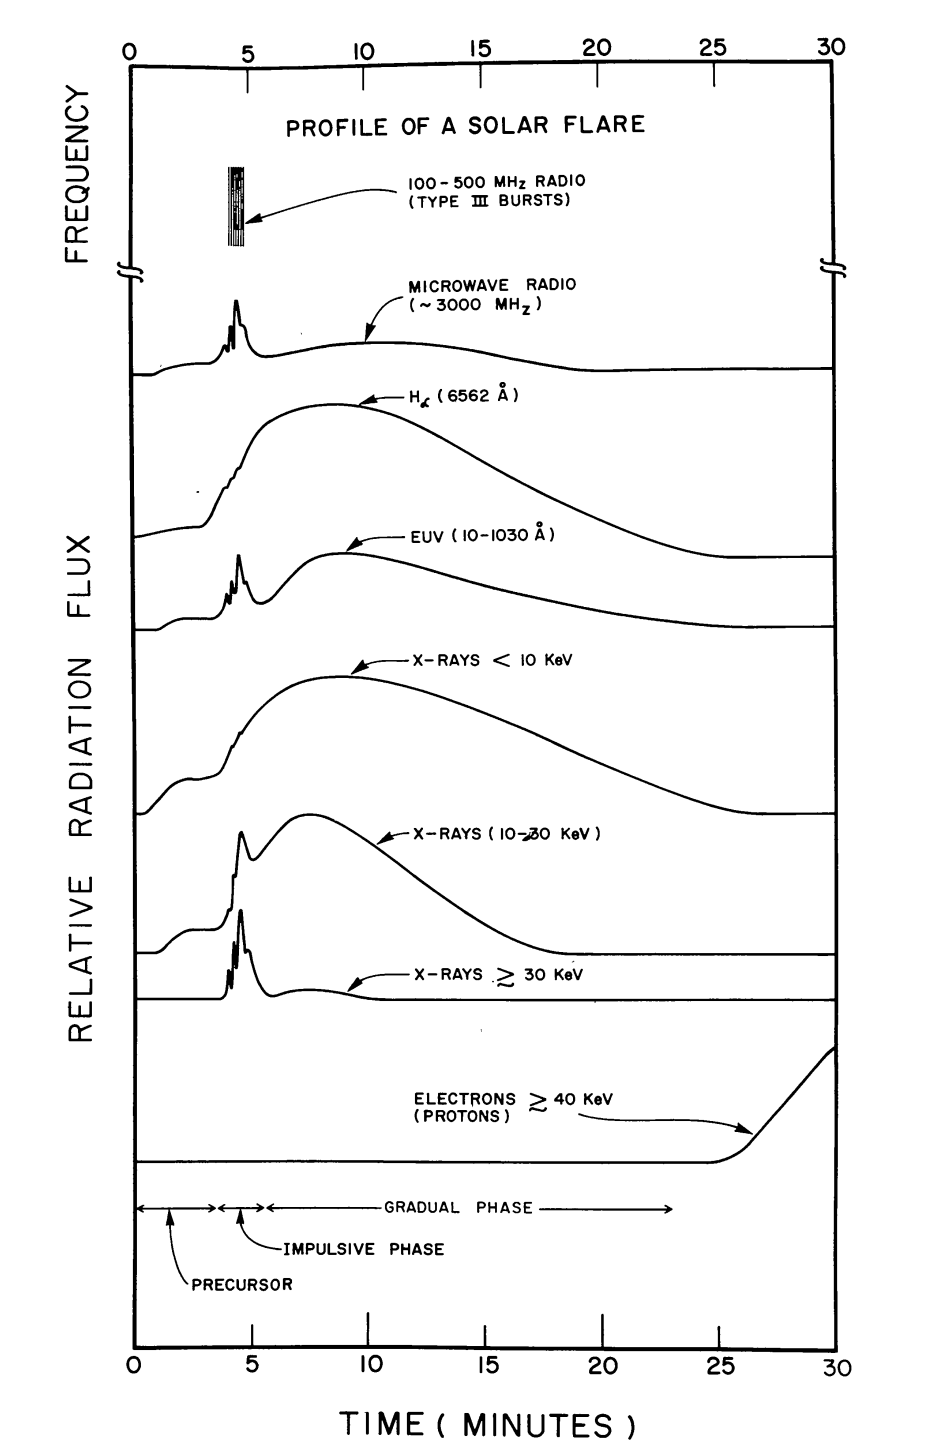
\includegraphics[width=0.4\linewidth]{figs/fig1}
	\caption{一个太阳耀斑在爆发相多波段电磁辐射变化图。来源: \textcite{Kane1974}}
	\label{fig:1}
\end{figure}



根据经典的二维CSHKP耀斑模型\parencite{Carmichael1964,Sturrock1966,Hirayama1974,Kopp1976}(见图\ref{fig:2})磁重联(\textit{magnetic reconnection})过程一般爆发在一对反向平行日冕磁感线形成的纤细的电流片中,并激发MHD激波\parencite{Shibata2011}。上方重联形成的磁感线可能携带着磁绳(\textit{flux rope})结构抛射而称为其他太阳活动(日冕物质抛射)的一部分。而下方的磁感线则连接形成了耀斑后环(\textit{post-flare loops}),这些环一般在软X射线(\textit{Soft X-ray, SXR}: $E<10$ KeV)波段被观测到,因而也被称为SXR环\parencite{Tsuneta1997,Zarro1999}。释放的日冕磁能加速了局地非热电子\parencite{Hudson2001,Tomczak2001,Krucker2007}。近期的射电观测也指出一部分电子可能被位于耀斑后环环顶的终止激波(\textit{termination shock})加速\parencite{Chen2015}。在耀斑环顶有一个硬X射线(\textit{Hard X-ray, HXR}: $E>10$ KeV)源\parencite{Masuda1994},一般认为可能来自一个高速喷流(\textit{jet})和环顶物质发生碰撞的过程\parencite{Shibata2011}。这些被加热的非热电子沿着磁感线向低层大气传播,轰击并加热低层大气。被迅速加热的色球(\textit{chromosphere})和过渡区(\textit{transition region, TR})大气产生了复杂的动力学与热力学效应。加热导致的压强增大推动一部分物质向上运动,被称为色球蒸发(\textit{chromospheric evaporation}, \cite{Fisher1985a,Fisher1985b,Fisher1985c}),这些高温等离子体填充了耀斑后环,产生了SXR辐射。在较大的色球蒸发过程当中,伴随着上百km$\ \mathrm{s}^{-1}$的物质上流\parencite{Milligan2006b},还会出现数十至上百km$\ \mathrm{s}^{-1}$的冷且致密的物质下流,被称为色球凝聚(\textit{chromospheric condensation}, \cite{Milligan2006a})。色球凝聚对一些色球谱线轮廓特征,如Mg \textsc{ii},Si \textsc{iv},和C \textsc{ii}的红翼不对称性的形成起了重要作用\parencites{Tian2015}。非热电子与致密的局地大气碰撞,在环的足点上产生了HXR辐射。加热的足点处色球和过渡区大气使的一系列形成与这些区域的谱线与连续谱辐射增强,这些位置也被称为耀斑带(\textit{flare ribbon})。具体增强的谱线有Balmer线系,Ca \textsc{ii}, Mg \textsc{ii}, C \textsc{ii}, Si \textsc{iv}, C \textsc{iv}等\parencite{Liu2015, Tian2015, Tian2018},如图\ref{fig:3}。其中一些的轮廓还出现了相当大的变化,如红蓝移,不对称性等\parencite{Li2015, Tei2018}。这些谱线的轮廓特征是我们理解太阳耀斑过程中的低层大气的演化过程的重要观测来源。

\begin{figure}
	\centering
	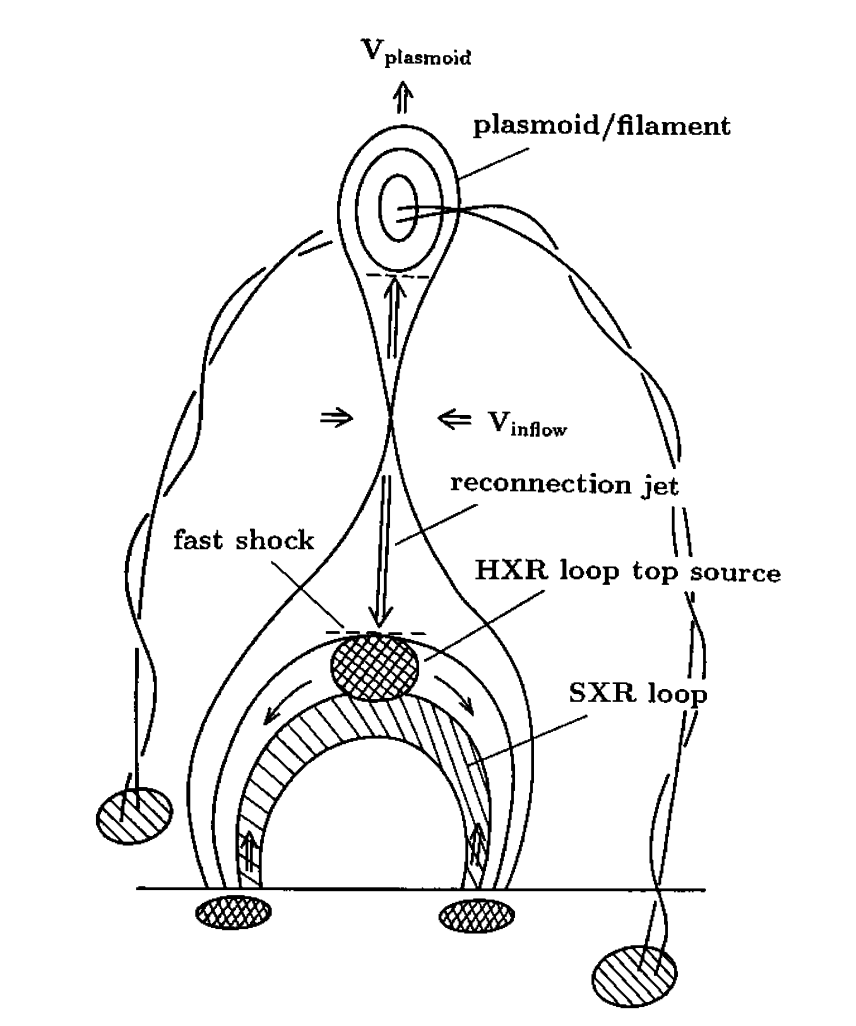
\includegraphics[width=0.5\linewidth]{figs/fig2}
	\caption{经典的二维CSHKP标准耀斑模型卡通图,加入了\textit{Yohkoh}卫星观测的新特征。来源:\textcite{Shibata1995}}
	\label{fig:2}
\end{figure}

\begin{figure}
	\centering
	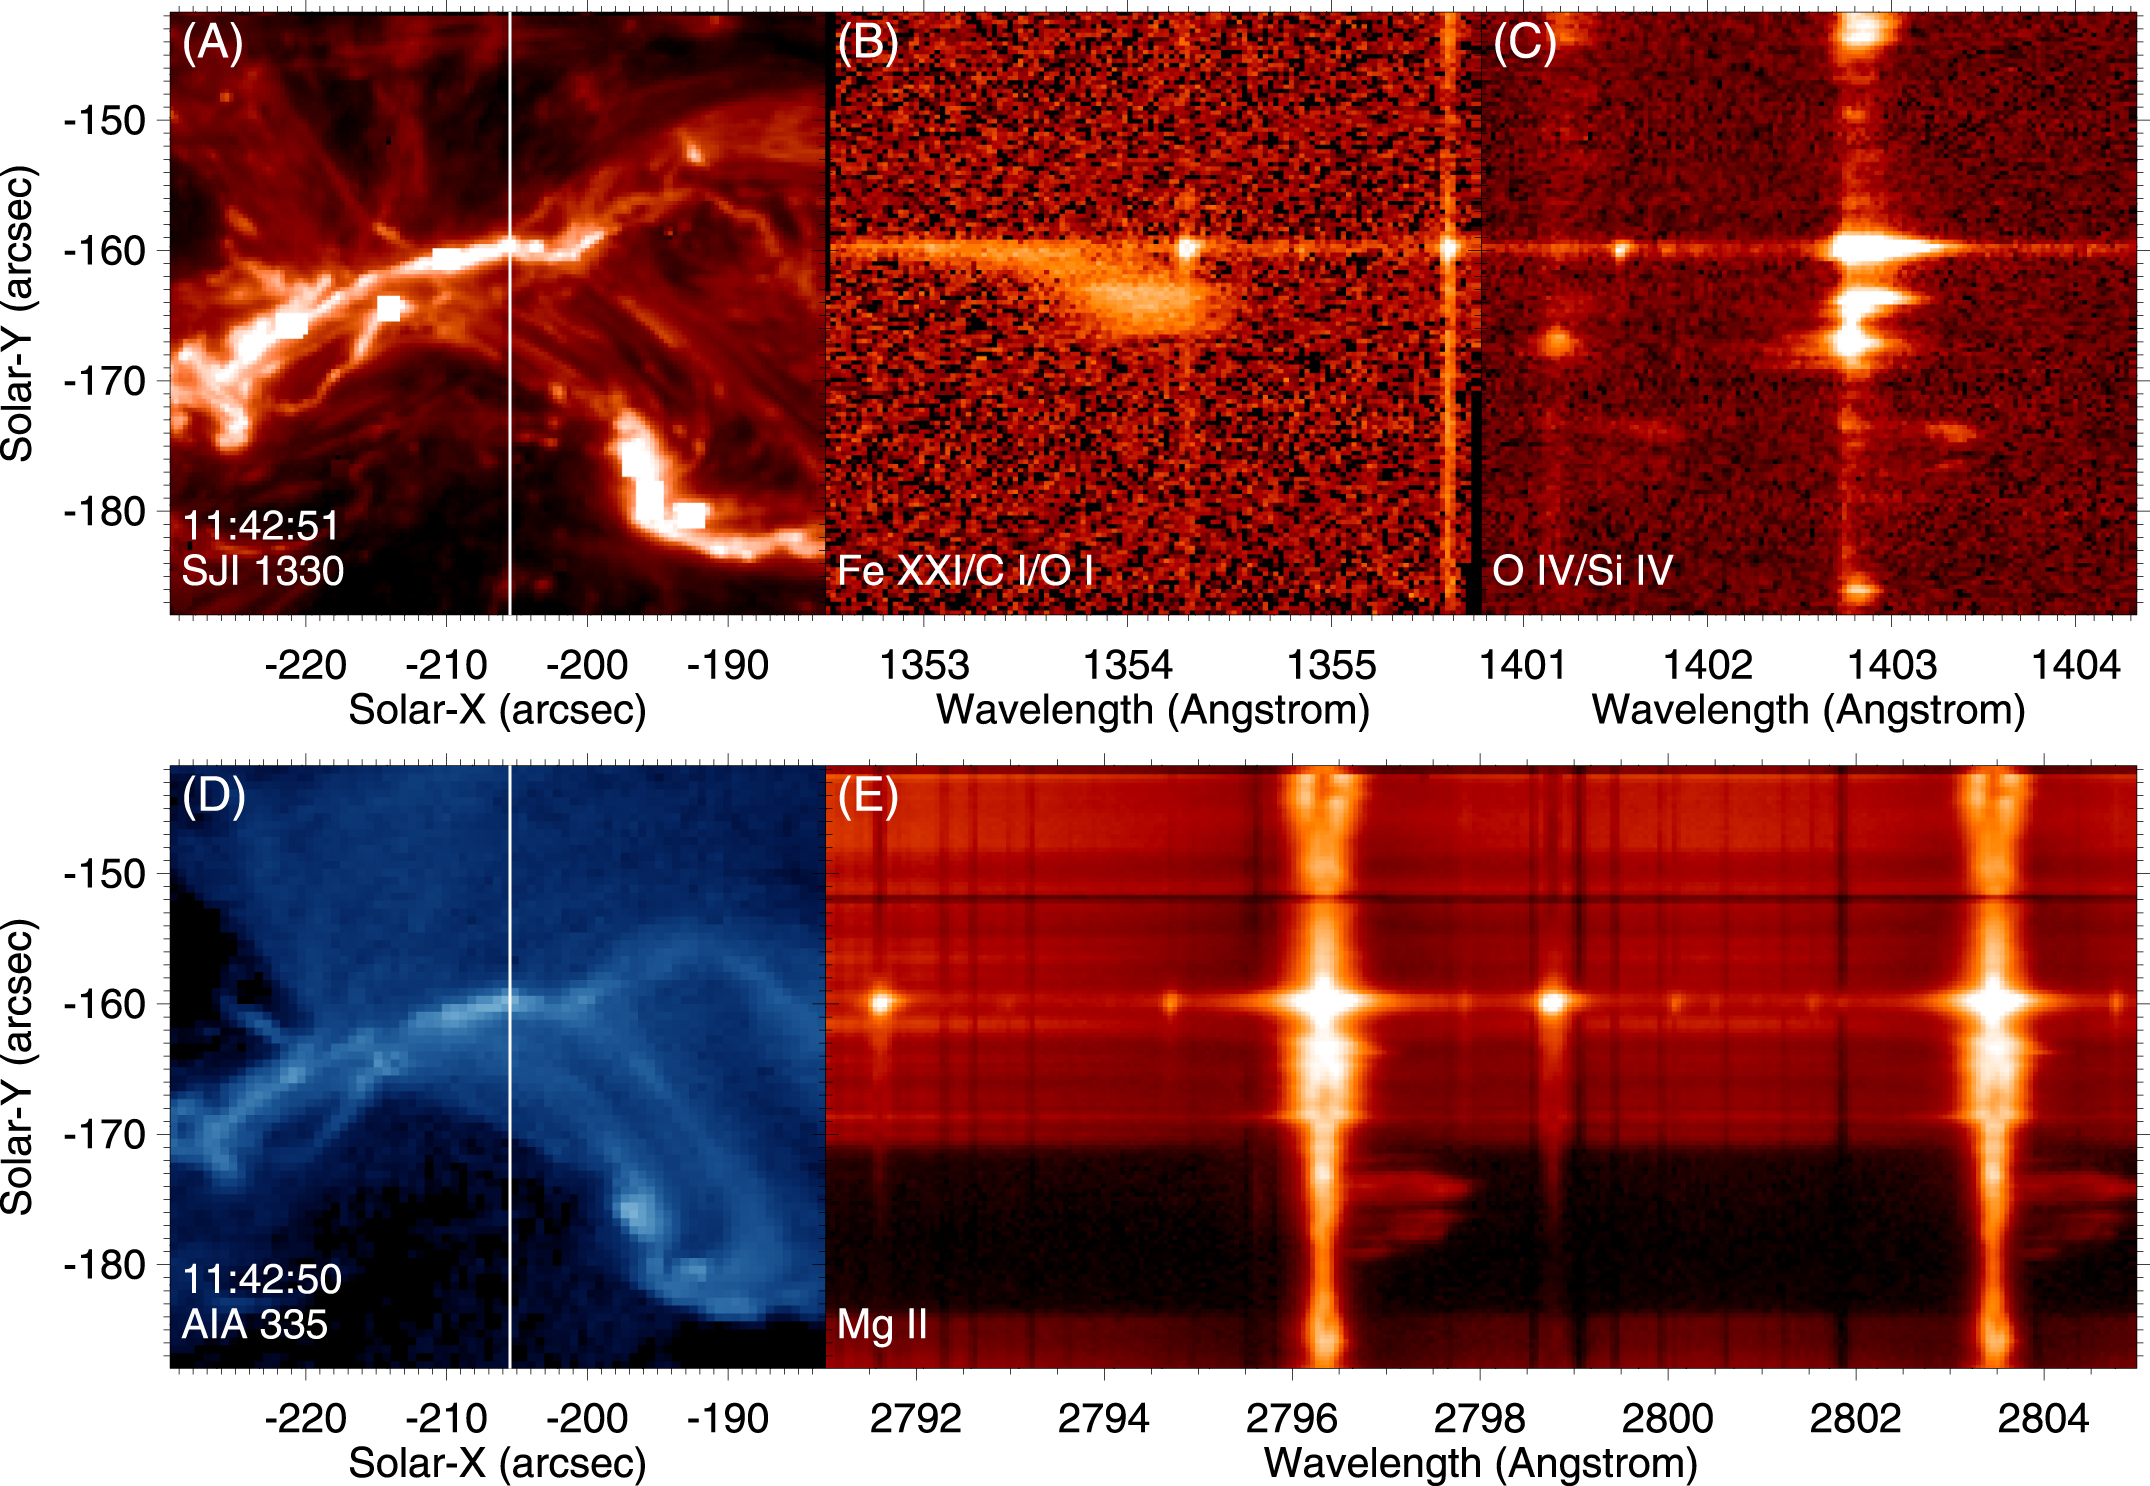
\includegraphics[width=0.7\linewidth]{figs/fig3}
	\caption{IRIS卫星对一个M1.6级耀斑带上谱线的观测,可以看到Si \textsc{iv},Mg \textsc{ii}等一系列谱线在耀斑带上都出现了红翼不对称性,而另一条高温谱线Fe XXI呈现出较大的蓝移。来源:\textcite{Tian2018}}
	\label{fig:3}
\end{figure}
另外近年来日冕中的三维磁重联过程也在极紫外(\textit{EUV})等一系列波段被观测到,这些耀斑不但具有复杂的日冕磁场拓扑结构,还表现出特殊的耀斑带形状,如环状耀斑带\parencite{Wang2012,Sun2013},J形耀斑带\parencite{Chandra2009}和X形耀斑带\parencite{Liu2016}等。这些特殊的耀斑带形状可以被一些三维的磁重联理论解释\parencite{Janvier2013,Janvier2014}。由于本文主要关注低层大气对入射非热电子束的动力学和热力学响应,因此对日冕中的三维磁重联过程及拓扑结构变化不再加以赘述。

对于这些低层大气的加热情况以及辐射转移的模拟也在近年来不断发展。以RADYN\parencite{Carlsson1992,Carlsson1997,Allred2005,Allred2015}为代表的一批辐射流体力学(\textit{radiative hydrodynamics, RHD})代码对我们认识耀斑加热时丰富的色球动力学过程提供了很大的帮助。通过计算色球中非局部热动平衡(\textit{nonlocal thermodynamics equilibrium, NLTE})条件下的辐射转移过程,我们得以了解色球中光学厚的一系列谱线的形成情况。关于这方面的研究成果,我会在\ref{sec:1.3}节中加以详细介绍。

\subsection{Ellerman炸弹}
Ellerman炸弹是太阳低层大气的爆发活动,最早在1917年被Ellerman在H$\alpha$线翼窄带滤光器的成像中观测到\parencite{Ellerman1917},表现为H$\alpha$线翼的增强\parencite{Georgoulis2002,Yang2003,Fang2006,Pariat2007,Nelson2013,Nelson2015,Vissers2015}。与之相反的,在H$\alpha$线心处一般观测不到增强。一般认为它们是太阳低层大气温度极小区(\textit{temperature minimum region, TMR})中的磁重联过程加热的结果\parencite{Reid2015,Rouppe2016,Ni2016}。其他形成于低色球的谱线,如Mg \textsc{ii}, Ca \textsc{ii}三重线也会在线翼出现增强,这些都被认为是低层大气加热的证据\parencite{Hong2017a,Nelson2017,Chen2017a},见图\ref{fig:4}。目前已有的一维辐射流体力学模拟和三维辐射磁流体力学(\textit{radiative magneto-hydrodynamics, RMHD})模拟,已经再现了Ellerman炸弹的部分光谱特征,如H$\alpha$的线翼增强等。\parencite{Hong2017a,Reid2017,Hansteen2017,Danilovic2017,Hansteen2019}。

\begin{figure}
	\centering
	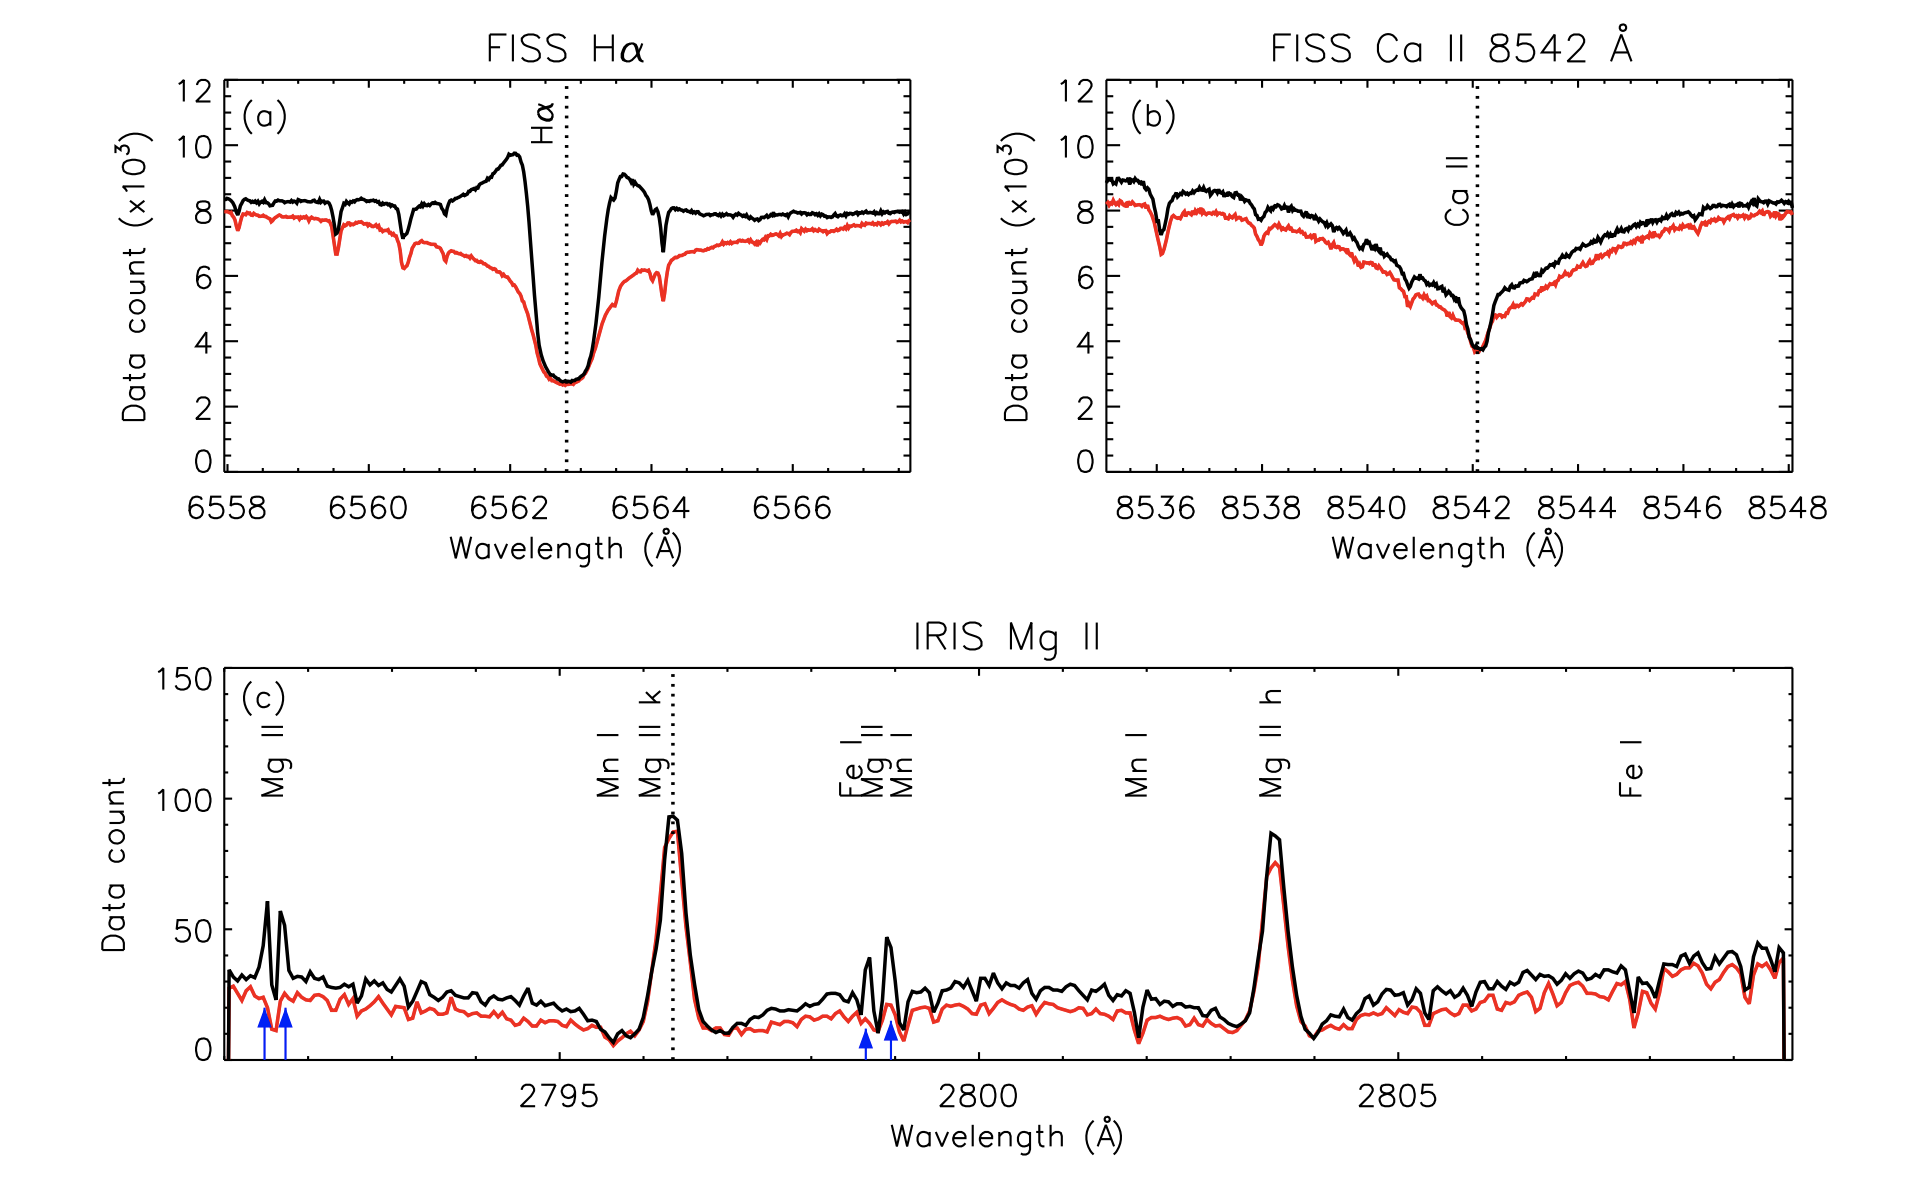
\includegraphics[width=0.8\linewidth]{figs/fig4}
	\caption{快速太阳成像光谱仪(\textit{Fast Imaging Solar Spectrograph, FISS})与IRIS卫星对一个Ellerman炸弹光谱的联合观测得到的光谱数据,红色和黑色的实现分别来自同一位置爆发前后的谱线轮廓。来源:\textcite{Hong2017a}}
	\label{fig:4}
\end{figure}
\subsection{紫外爆发}
紫外爆发(\textit{UV burst})是近年来新被观测到的一种位于色球层的小规模爆发活动,最早被过渡区成像摄谱仪(\textit{Interface Region Imaging Spectrograph, IRIS}: \cites{DePontieu2014})卫星于2014年在1400 \mbox{\AA}波段成像观测到\parencite{Peter2014},在最初也被称为热爆发(\textit{hot explosion}, \cite{Peter2014})和IRIS炸弹(\textit{IRIS bomb}, \cite{Tian2016})。紫外爆发经常出现在IRIS卫星对活动区(\textit{active region, AR})的观测当中\parencite{Tian2016,Polito2016,Hou2016}。在光谱观测上,紫外爆发表现为Si \textsc{iv} 和 C \textsc{ii}谱线的剧烈增强和致宽,其等值宽度能够达到$50-200\ \mathrm{km}\ \mathrm{s}^{-1}$, 同时在致宽的Si \textsc{iv} 1394\mbox{\AA}线上还经常能够观测到一条Ni \textsc{ii}的吸收线\parencite{Peter2014,Chen2019a},见图\ref{fig:5}。一般认为紫外爆发的能量来源于Ellerman炸弹类似,都来自于低层大气中的磁重联过程\parencite{Peter2014,Tian2018b},见图\ref{fig:6}。
\begin{figure}
	\centering
	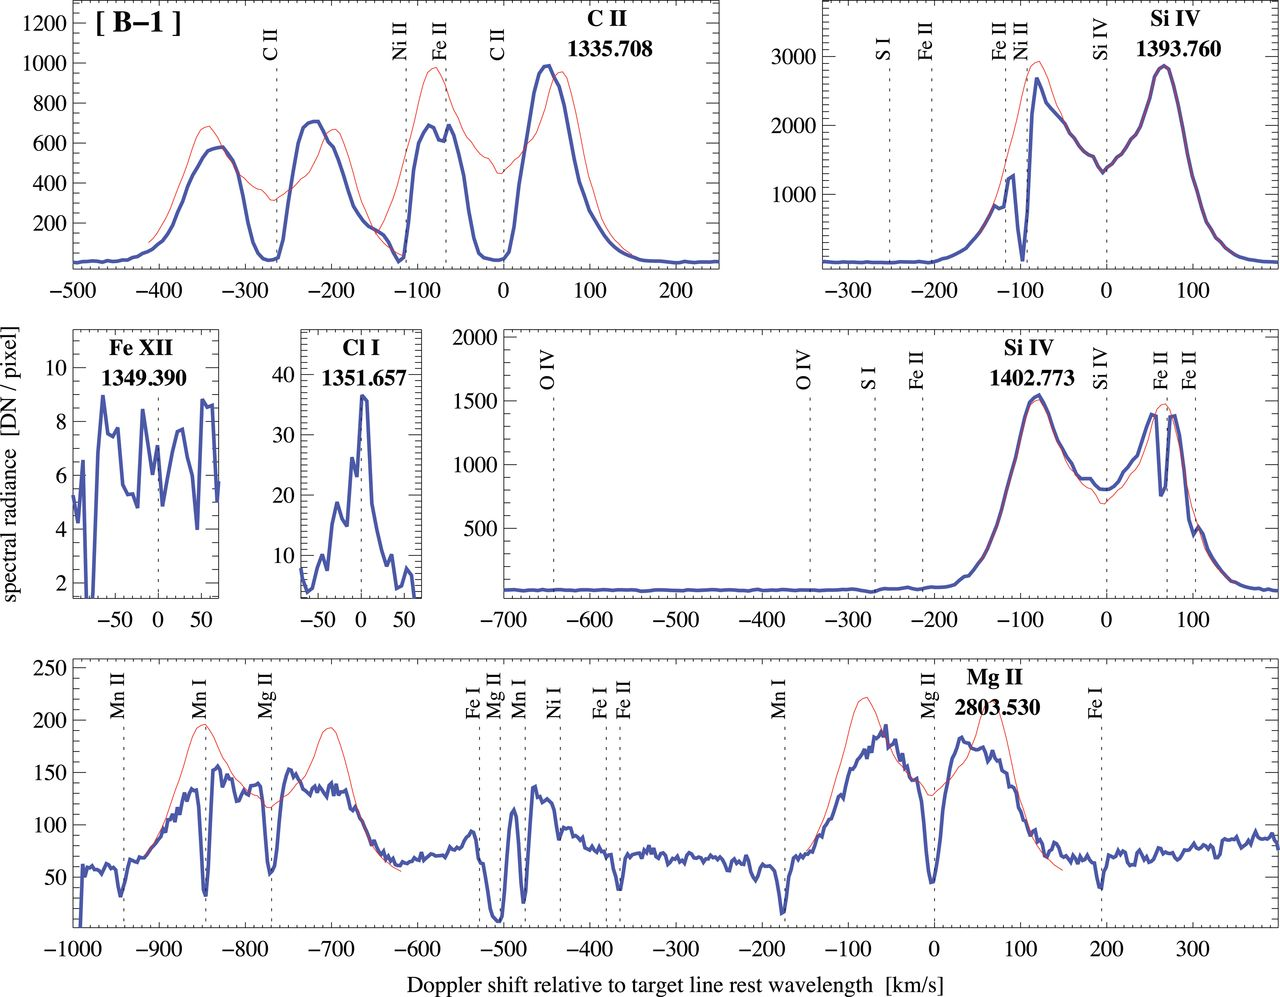
\includegraphics[width=0.7\linewidth]{figs/fig5}
	\caption{IRIS卫星观测到的紫外爆发的光谱。来源:\textcites{Peter2014}}
	\label{fig:5}
\end{figure}
\begin{figure}
	\centering
	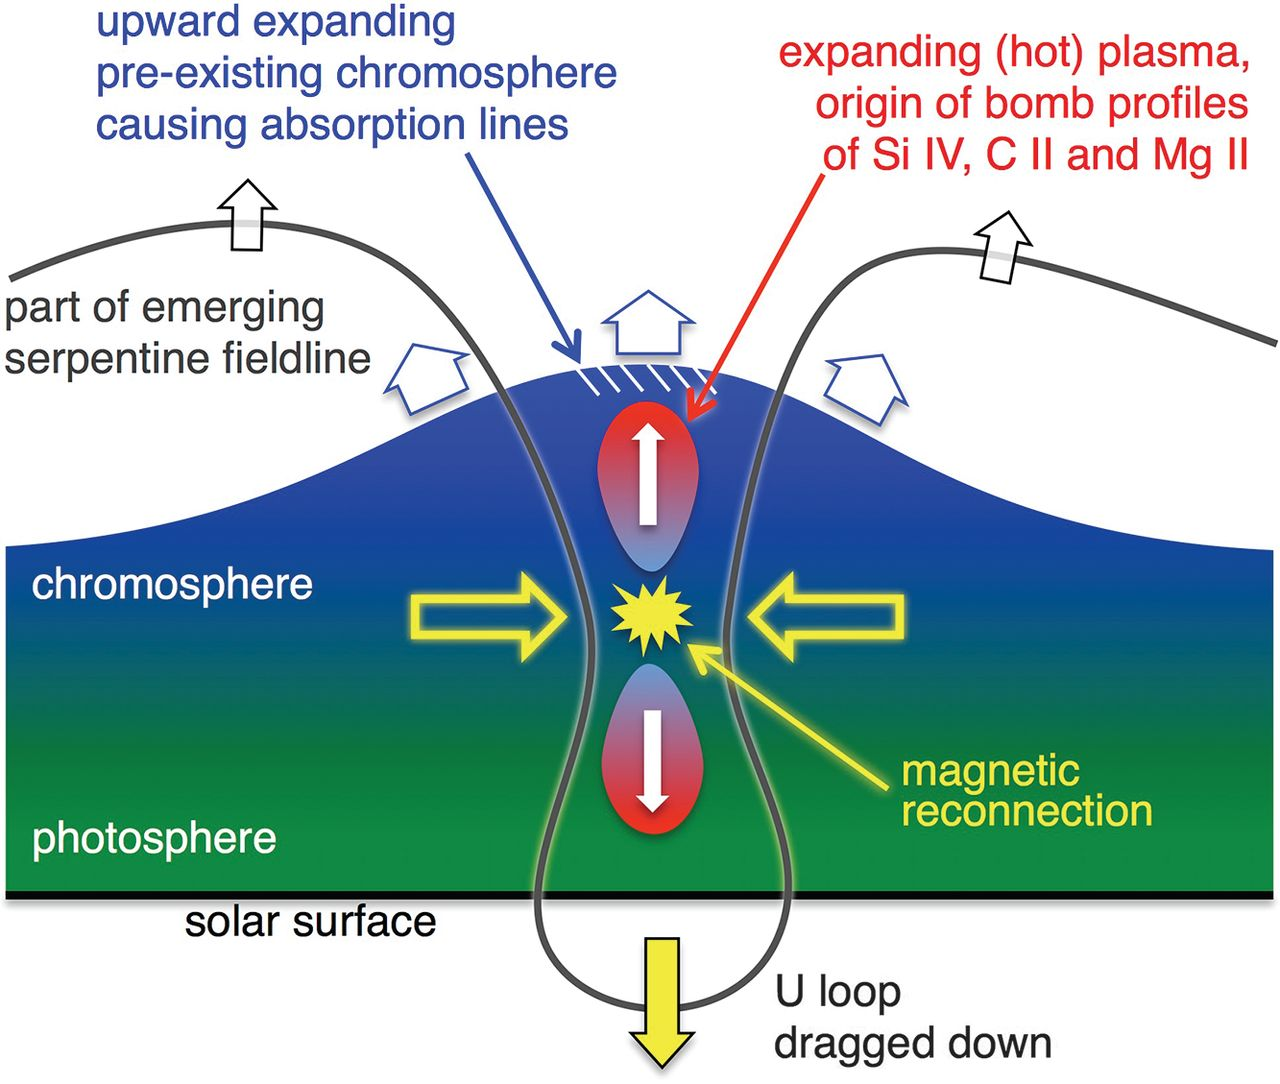
\includegraphics[width=0.7\linewidth]{figs/fig6}
	\caption{一个用于解释紫外爆发成因的卡通图。\textcite{Peter2014}认为色球层中的倒U型磁感线间的磁重联过程加热了局部色球大气,这些物质的向上蒸发导致了急剧增强和致宽的Si \textsc{iv}, C \textsc{ii}等线。在这些蒸发物质的上方存在的较冷的色球大气造成了Ni \textsc{ii}等覆盖在发射谱线上的吸收特征。来源:\textcites{Peter2014}}
	\label{fig:6}
\end{figure}

近年来的一些观测表明,紫外爆发和Ellerman炸弹存在着一定的关联性\parencite{Vissers2015,Tian2016},它们的形成机制也有一定的相似之处。\textcite{Fang2017}表明发生在低层大气的Ellerman炸弹并不足以加热附近的温度极小区到达$10^4$ K,进而电离足够的Si \textsc{iv}离子产生Si \textsc{iv}谱线增强。\textcite{Chen2019a}对Goode太阳望远镜观测到的161个Ellerman炸弹进行了统计分析,发现仅有约20个Ellerman炸弹能够在IRIS卫星观测中找到对应的紫外爆发,而且这些紫外爆发往往位于对应的火焰状Ellerman炸弹的上方。他们指出这些相关的Ellerman炸弹和紫外爆发可能形成发生在同一个电流片上的在不同高度的磁重联过程中(见图\ref{fig:7})。Hansteen等人近年来一直使用Bifrost三维辐射流体动力学代码对Ellerman炸弹和紫外爆发的光谱特征进行计算,也成功再现了Si \textsc{iv},H$\alpha$等一系列谱线轮廓特征。他们发现紫外爆发和Ellerman炸弹可以是在空间和时间上都不关联的两个爆发活动\parencite{Hansteen2017},但它们也可以同时形成在同一狭长电流片的两端\parencite{Hansteen2019}。
\begin{figure}
	\centering
	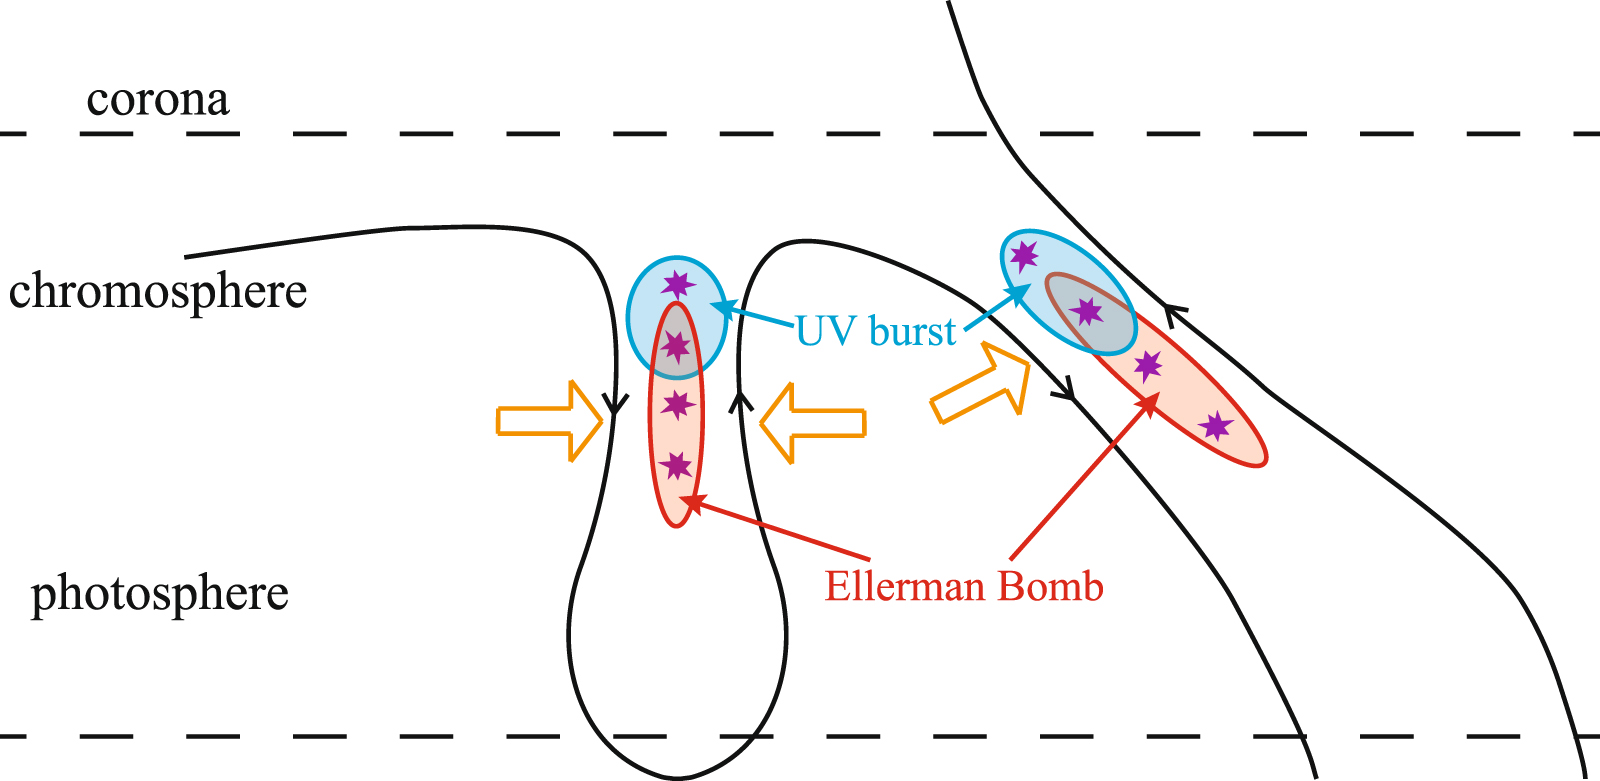
\includegraphics[width=0.7\linewidth]{figs/fig7}
	\caption{一个用以解释Ellerman炸弹与紫外爆发形成在同一电流片上的卡通图。来源:\textcites{Chen2019a}}
	\label{fig:7}
\end{figure}
\subsection{M矮星上的恒星耀斑}
近年来,随着地基和太空望远镜的发展,恒星耀斑也越来越多地被在测光(\textit{photometric})和分光(\textit{spectroscopic})观测中被探测到,并且展现出特殊的辐射特征。尤其是在一些M矮星上,如UV Ceti,YZ CMi和比邻星上都观测到了较强的白光耀斑,释放出比太阳耀斑高出一个量级以上的能量\parencite{Haisch1989}。统计研究表明光谱型介于dM3e-dM6e间的M矮星常常能观测到频繁的耀斑爆发\parencite{Lacy1976}。这些耀斑的光变曲线和太阳耀斑类似,都包含了一个快速增长的爆发相和一个持续几十分钟到几个小时的衰变相\parencite{Moffett1974,Moffett1976}。

在测光观测上,随着Kepler卫星\parencite{Borucki2010}的发射,大视场长周期的白光观测在M矮星和一些类太阳的G型星上都观测到了大量的耀斑活动和恒星黑子\parencite{Shibayama2013,Hawley2014,Davenport2014,Lurie2015,Yang2017}。这些白光耀斑往往在U波段(3200\mbox{\AA}-4000\mbox{\AA})光度学观测上显示出比较大($\Delta U\sim5\ \mathrm{mag}$)的变化\parencite{Haisch1989}。同时宽波段(U,B,V和R)的测光观测指出耀斑在白光波段的增强可能与一个$T\sim 9000-10000$ K的黑体谱相似\parencite{Hawley1991,Hawley1992}。在2018年发射的凌星系外行星巡天望远镜(\textit{Transiting Exoplanet Survey Satellite, TESS}: \cites{Ricker2014})发射开始观测后的两个月内,利用其高分辨率(2分钟)的观测数据,就发现了632颗发生过耀斑活动的M矮星\parencite{Gunther2019}。这些数据充分说明了频繁的恒星活动对系外行星宜居性的重要影响。

相比于长周期和大视场的测光巡天,恒星耀斑的分光观测往往较为困难,因为它们的出现往往是不可预测的。一般来说耀斑事件都伴随着连续谱增强及H$\alpha$等Balmer线系,Ca \textsc{ii}, Mg \textsc{ii},He \textsc{i}, K \textsc{i}等一系列色球谱线的增强和致宽\parencite{Eason1992}。\textcite{Hawley2007}利用Hubble太空望远镜上的空间望远镜成像光谱仪(\textit{Space Telescope Imaging Spectrograph, HST/STIS})观测了YZ CMi上的一个恒星耀斑的NUV光谱中的Mg \textsc{ii}和Fe \textsc{ii}线。其中Mg \textsc{ii}线展现出了剧烈的增宽,其半高全宽(\textit{full width at half maximum, FWHM})一度达到了250 $\mathrm{km}\  \mathrm{s}^{-1}$。YZ CMi上的白光耀斑和太阳上的\textsc{i}型白光耀斑类似,在Balmer系限3646\mbox{\AA}附近出现蓝段连续谱辐射的突然增强,被称为Balmer跳跃\parencite{Kowalski2010}。Balmer跳跃一般认为来自于氢原子与自由电子的复合(\textit{recombination})过程,因此着预示着白光连续谱不仅具有一个黑体谱的成分,还有来自于氢原子复合连续谱的分量\parencite{Kowalski2012}。\textcites{Kowalski2013}对20个M矮星上的恒星耀斑进行了光谱和光度的联合观测,他们发现可见光谱在$4000-4800$\mbox{\AA}间的部分可以被一个温度较高的9000-14000 K的黑体谱所拟合,而$\lambda>4900$ \mbox{\AA}的光谱则可以被一个温度较低$\sim6000$ K左右的黑体谱拟合。在这些耀斑中的Balmer线系谱线的线翼都出现了吸收的现象,这一特征被认为是低层大气被加热的证据。他们最近对两个发生在一个dM4e型矮星上的耀斑进行了联合观测,并首次利用Hubble太空望远镜上的宇宙起源光谱仪(\textit{Cosmic Origin Camera, HST/COS})获得了耀斑在大部分NUV波段的光谱数据,包含了增强的Balmer连续谱和大量的Fe \textsc{ii}和Mg \textsc{ii}线\parencite{Kowalski2019}。根据这些多波段的光谱观测,他们发现$T = 9000$ K的黑体谱并不能很好的拟合这两个耀斑事件的连续谱,尤其是在NUV波段。\textcite{Froning2019}对另一颗M矮星GJ 674的观测更揭示了耀斑过程中大量的FUV发射线,如Si \textsc{iii},O \textsc{iii},C \textsc{iii},Fe \textsc{xxi}等。

对这些M矮星耀斑的辐射流体力学模拟也同太阳耀斑模拟一样在近年来不断发展,不过目前主要还停留在再现恒星耀斑中的可见光连续谱和Balmer系谱线轮廓上。早期利用RADYN进行的模拟揭示了一系列增强的谱线,如H$\alpha$,H$\beta$, Ca \textsc{ii} H和K,He \textsc{ii} 304\mbox{\AA}等,但未能再现辐射温度较高的黑体连续谱\parencite{Allred2006},且不能再现剧烈致宽的Mg \textsc{ii}线\parencite{Hawley2007}。Kowalski等人在后来发现,要想再现这样剧烈增强的连续谱,需要在模拟中引入较高能量的非热电子束($1\times10^{13}\ \mathrm{erg}\ \mathrm{s}^{-1}$,以下简称F13,比普通太阳耀斑的模拟高至少两个量级,参见\cite{Kowalski2015})。同时使用一些更精确的Balmer线系的Stark致宽效应的计算方法,对整个耀斑的在3500 \mbox{\AA}-5000 \mbox{\AA}的连续光谱和Balmer发射线取得了非常好的拟合效果\parencite{Kowalski2015,Kowalski2016,Kowalski2017b}。和太阳耀斑类似,在M矮星的高非热电子能流模拟中也得到了色球凝聚的结果。这些模拟结果得到的大气参量可以帮助我们估计可见光和NUV波段的光学深度,Balmer跳跃比和色球凝聚处的电子密度等\parencite{Kowalski2018a}。
\section{辐射转移与谱线形成理论简介}
辐射转移(\textit{radiative transfer, RT})是恒星大气中重要的物理过程,最早由Schuster在1905年归纳给出辐射转移方程\parencite{Schuster1905}。它既是恒星大气中能量传输(加热、冷却)的重要手段,又是天体物理中绝大多数观测量即电磁波谱的形成机制。正确地理解辐射转移过程,不仅有助于我们处理流体力学方程组中能量方程的辐射项,又能够直接合成光谱和我们观测到的电磁波谱中的各种特征(连续谱、谱线等)进行比较,直接检验我们对太阳爆发时低层大气认识的正确性。在这一部分,我将介绍与辐射有关的物理量与辐射转移方程。谱线轮廓形成和致宽的机制和存在磁场情况下对光的偏振参数影响。限于篇幅,研究内容和个人能力限制,对辐射转移过程的介绍是比较简单的:我只介绍一维平面平行层大气的辐射转移过程,且只涉及静态大气不含时的辐射转移方程(事实上在模拟中存在速度场,显然不能以静态大气处理)。另外,我们讨论的主要是宏观上的辐射转移,即用一些宏观测量量来描述辐射场,而非光子数密度这样的微观量,尽管光子的概念在谱线形成的过程中仍然非常重要。本节的主要内容及公式都来自于Hubney和Mihalas所著的《Theory of Stellar Atmospheres》一书\parencite{Mihalas2014}。
\subsection{辐射转移方程}\label{subsec:1.2.1}
在介绍辐射转移方程之前,有必要介绍一些描述辐射场的物理量和重要概念:

\noindent
\textbf{辐射强度(Intensity)}\ \ 我们通过衡量单位时间$\delta t$通过单位面元$\delta\boldsymbol{A} $以某个方向$\boldsymbol{n}$通过单位立体角$\delta \Omega$在频率区间$(\nu,\nu+\delta\nu)$的辐射能量$\delta E$来衡量辐射强度的大小,即
\begin{equation}
	I(\boldsymbol{x},t,\boldsymbol{n},\nu ) = \frac{\delta E}{\delta t  \delta \Omega \delta \nu \delta\boldsymbol{A} \  \boldsymbol{n}}
\end{equation}
其在SI单位制下的单位为$\mathrm{W}\ \mathrm{m}^{-2}\ \mathrm{Hz}^{-1}\ \mathrm{sr}^{-1}$,在CGS单位制下单位为$\mathrm{erg}\ \mathrm{s}^{-1}\ \mathrm{cm}^{-2}\ \mathrm{Hz}^{-1}\ \mathrm{sr}^{-1}$。

\noindent
\textbf{辐射流量(Flux)}\ \ 辐射流量$\boldsymbol{F}_{\nu}$被定义为使得$\boldsymbol{F}_{\nu}\ \md \boldsymbol{A}$给出单位时间内通过面元的在频率间隔$\md \nu$内的能流,因此我们要对单位角进行积分
\begin{equation}
	\boldsymbol{F}_{\nu} = \oint_{4\pi} I_{\nu}(\boldsymbol{n} )\boldsymbol{n}\md \Omega
\end{equation}
在恒星当中,由于我们往往只对向观测者方向传播的能量感兴趣,因此观测到的辐射流量一般只积$\theta\in (0,\pi/2)$之间。

\noindent
\textbf{局部热动平衡(Local Thermodynamic Equilibrium, LTE)}\ \ 在恒星大气物理的研究当中,局部热动平衡是永远无法回避的一个概念。我们大多数关于辐射场和原子电离激发的知识是适用于平衡态的,如Boltzmann分布和Saha方程等。但是显然恒星大气存在温度梯度,并不是一个完全的热平衡态。为了做出一个合适的近似,一个很自然的想法是,如果局部的温度梯度和密度梯度是\emph{充分小}的,且粒子密度\emph{充分大}以保证充分的碰撞,那么我们就可以用一些“局部”的大气动力学、热力学参数来描述一个“局部”范围内的大气,并认为这个范围内的大气处于一个平衡态当中,这就是局部热动平衡的概念。这个“充分小”可以理解为温度和密度的标高应该远大于粒子的自由程\parencite{Mihalas2014}。但是我们也应该注意到光子很可能拥有比普通粒子大的多的自由程,因为整个外辐射场是通过一系列辐射与吸收机制(对应粒子的电离、受激、复合和退激发过程)与粒子耦合在一起来趋向平衡态的。因此检验这个近似是否在恒星大气中严格成立事实上在不依靠数值模拟的情况下是比较困难的。

总的来说,局部热动平衡在恒星大气的光球是一个比较好的近似,但是在色球很可能不是,这也是为什么我们需要非局部热动平衡(\textit{non-LTE, NLTE})的概念\parencite{Mihalas2014}。理论上来说,任何对于LTE的偏离都应该算作NLTE的范畴内,但是在具体代码计算中,比较常用的方法是假设粒子的速度分布仍然满足平衡态下的Maxwellian分布,但原子能级粒子数分布则可以偏离Boltzmann分布和Saha方程给出的限制\parencites{Kubat2014}。由于此时的能级粒子数分布应该由动理学平衡(\textit{kinetic equilibrium})方程给出,因此此时也被称为统计平衡(\textit{statistical equilibrium})或动理学平衡\parencites{Mihalas2014}。

\noindent
\textbf{吸收(Absorption),发射(Emission)与散射(Scattering)}\ \ 当一个光子和粒子相互作用而消失的时候,我们一般说它被\emph{吸收}了。而如果粒子失去一部分能量而释放出一个光子,我们就称之为\emph{发射}。如果这个光子的能量一部分通过碰撞激发与电离进入交换给了其他粒子,那么我们一般称这是\emph{热(真)吸收}(\textit{thermal absorption})。反之,如果它激发了一个原子从某个能级$l$跃迁到$u$,而这个原子又很快退激发回到$l$发出一个频率大致相等的光子,那么这个过程应该被称作\emph{散射}(\textit{scattering}),因为光子的能量并没有介入到粒子的内能中去。这两个过程的重要区别是热吸收的再辐射应该是遵循处于热动平衡下的辐射场性质的,而散射过程的再辐射却不遵循这些性质。

然而,我们应该指出,在真实情况下,由于原子有着复杂的能级和电离结构,一个光子被吸收然后再被释放的中间过程是非常复杂的,很难直接用吸收或者散射的概念来严格描述。在某些情况下,如果只考虑光子被吸收的过程而不考虑它是如何再发射的,我们会宽泛地把散射过程也归纳到吸收中来考虑。

对于造成光子被吸收和发射有着各种各样的物理过程,我们不再这里对它们的物理形式做过多的数学描述,只是走马观花式地罗列恒星大气中可能造成吸收的物理过程。可以吸收或辐射宽波段光子的过程一般包括\parencite{Wang1993}:
\begin{itemize}
	\item 光致电离与复合(\textit{photoionization, recombination})
	\item 自由-自由跃迁/轫制辐射 (\textit{free-free transition/bremsstrahlung})
	\item 分子离解、电离和分子带吸收
	\item Thompson散射与Rayleigh散射
	\item 尘埃的散射和吸收
\end{itemize}
而与之相对应的就是谱线内部的跃迁(\textit{bound-bound transition})。具体而言,包含自发辐射(\textit{spontaneous emission}),受激辐射(\textit{stimulated emission})与光致激发(\textit{photoexcitation})。


现在我们可以开始讨论一维平面平行层大气辐射的传播过程应该用什么样的方程和参量来描述了,为了定量描述辐射在局地的吸收和发射过程,我们可以定义两个参量,\emph{不透明度}$\chi_\nu$(\textit{opacity})与发射系数$\eta_\nu$(\textit{emissivity})。前者描述了单位的辐射强度通过单位距离后的改变量。在考虑散射的情况下而后者描述了辐射通过单位距离物质之后的增强量,考虑这两个参数同时对辐射强度的影响,我们有
\begin{equation}
	\md I_{\mu\nu} = \left(\eta_{\nu} - \chi_{\nu}I_{\mu\nu}\right) \mu \md z
\end{equation}
其中$\mu=\cos\theta$表示辐射出射方向与平面大气法线方向的夹角的余弦,$z$表示大气高度,$I_{\mu \nu}$表示以某一方向出射的辐射强度。注意我们为了尽可能简单的提取辐射转移的物理特征,在写下这个方程的时候已经做了非常多的假设。其中最重要的假设是吸收和发射都是\emph{各向同性的}。事实上这是一个并不好的假设,因为显然一系列散射过程,如Thompson散射的再发射系数就是非各向同性的。下面我们继续改写这个方程,两边同除$\chi_\nu \mu \md z$,得到
\begin{equation}
	\mu \frac{\md I_{\mu \nu}}{\chi_\nu\md z} = \frac{\eta_\nu}{\chi_\nu} - I_{\mu \nu}
\end{equation}
下面我们定义另外两个重要的参量,光学深度(\textit{optical depth}) $\md \tau_\nu \equiv \chi_\nu \md z$与源函数(\textit{source function}) $S_\nu \equiv \eta_\nu / \chi_\nu$。前者为我们提供了判断一条谱线辐射转移中吸收是否重要的判据。一般来说$\tau = \int \chi_\nu \md z > 1$时,我们称之为光学厚(\textit{optically thick}),说明谱线形成中的吸收是不可忽略的。反之则称之为光学薄(\textit{optically thin}),说明吸收过程并不重要。此时我们观测到的谱线内的辐射可以直接理解为视线方向上所有发射的积分。而后者从形式上来看表示的是发射和吸收之比,但其还有一个重要的物理意义,即\emph{单位光深所能发射出的光子数}\parencites{Mihalas2014}。所以现在方程写作
\begin{equation}
	\mu \frac{\md I_{\mu \nu}}{\md \tau} = S_{\nu} - I_{\mu \nu}
\end{equation}
这一方程对出射辐射的形式解为
\begin{equation}
	I_{\mu \nu} = \frac{1}{\mu} \int^\infty_{\tau_\nu} S_{\nu} e^{-(t_\nu - \tau_\nu)} \md t_\nu \label{eq:1.6}
\end{equation}
由于$S_{\nu}$也是光学深度$\tau_\nu$的函数,所以这仍然是一个形式解。但从这个解的形式可以看出,与一般的流体力学方程不同,想要计算出射的辐射强度,这个积分将涉及整个太阳大气,因此求解这样的方程是非常消耗计算时间的。最后我们讨论一下同时考虑热吸收和散射时和LTE假设下的源函数的形式。在LTE下,热吸收和热发射应该遵循热平衡下的辐射场性质(即Kirchhoff热辐射定律) $\eta_{\nu,\mathrm{thermal}}/\chi_{\nu,\mathrm{thermal}} = B_{\nu}$,其中$B_\nu$为Planck函数。我们可以把$\eta_\nu$和$\chi_\nu$分解写成热吸收和散射两个部分
\begin{align}
	\chi_\nu &= \kappa_\nu + \sigma_\nu \\
	\eta_\nu &= \kappa_\nu B_\nu + \sigma_\nu J_\nu
\end{align}
其中$\kappa_\nu$和$\sigma_\nu$分别代表热吸收和散射的吸收系数,$J_\nu$代表立体角平均后的辐射强度。因此在这样的近似下源函数的形式可以写成\parencites{Mihalas2014}
\begin{align}
	S_\nu &= \frac{\kappa_\nu B_\nu + \sigma_\nu J_\nu}{\kappa_\nu + \sigma_\nu} \nonumber \\
	& = \epsilon_\nu B_\nu + (1-\epsilon_\nu )J_\nu
\end{align}
\subsection{谱线形成分析}\label{sec:1.2.2}
太阳上的原子谱线最早被Fraunhofer在1814年观测到,这也是最早被观测到的原子能级跃迁产生的吸收线。那么如何判断一条谱线是在太阳大气的何种高度,进一步的,何种大气参数下形成的呢?一个简单的想法是根据太阳大气的温度分布,依照原子电离态可能在何种温度区间下存在的信息,进而粗略地推断谱线的形成高度。这显然是一个非常粗略的方法,而且对于吸收效应比较重要的谱线,即光学厚的谱线,我们观测到的光子往往是经过了多次的散射过程才形成的。在这样的情况下,我们观测到的谱线轮廓中的光子往往仅形成在整个电离态原子可能存在高度的较高处。对于这些谱线,基于\ref{subsec:1.2.1}节中讨论的辐射转移方程,我们可以把光学深度$\tau_\nu = 1$的高度当作是谱线形成的特征高度,因为此处发射的光子大约有$1 - e^{-1}\approx63\%$可以被我们观测到。下面为了更好的确定整个谱线的形成区间,并对谱线形成高度的大气参数进行一个定量分析,我们介绍一种基于贡献函数$C_{I}$\parencite{Magain1986,Carlsson1997,Kowalski2015}的方法。

首先我们把辐射转移方程形式解式\eqref{eq:1.6}中的被积函数定义为贡献函数$C_I(\mu,z) \equiv \md I_{\mu \nu}/\md z = \chi_\nu S_\nu e^{-(t_\nu-\tau_\nu)}$,因此所有的出射辐射强度可以视作整个贡献函数对大气高度的积分。自然地,贡献函数大的地方就应该是谱线真正形成的地方。为了更加定量的描述这一点,我们可以定义一个积累(\textit{cumulative})贡献函数$C'_I(\mu,z)$\parencite{Kowalski2016b}。
\begin{equation}
    C'_I(z,\mu) = 1- \frac{\int^{z'=z_{\mathrm{max}}}_{z' = z} C_I(z',\mu)\ \mathrm{d}z'}{\int^{z'=z_{\mathrm{max}}}_{z' = z_{\mathrm{min}}} C_I(z',\nu)\ \mathrm{d}z'}
\end{equation}
这是一个归一化的函数,进一步的,我们可以定义$C'_I \in (0.05,0.95)$作为谱线的形成区间。另外我们可以利用贡献函数$C_I$作为一个权重函数,对模拟中的大气参数在高度上做加权平均,作为谱线形成区间内的典型大气参数,即
\begin{equation}
    <X> = \frac{\int^{z\left(C'_I=0.95\right)}_{z\left(C'_I=0.05\right)}C_I(z',\mu)X\ \mathrm{d}z'}{\int^{z\left(C'_I=0.95\right)}_{z\left(C'_I=0.05\right)}C_I(z',\mu)\ \mathrm{d}z'}
\end{equation}
其中$X$可以是温度、电子密度和速度等一系列参量。
\subsection{谱线的致宽}\label{sec:1.2.3}
尽管我们知道原子跃迁的能级差应该是确定的,但是观测到的谱线永远不会是一个$\delta$函数。除了测量造成的致宽之外,有许多物理效应可以造成谱线在辐射转移过程中的致宽。在这一小节,我会对谱线的致宽机制和谱线形状做出一个简单的总结。我将回避复杂的数学推导而尽量给出一个直观的物理图像和最后的数学结论。
\newline
\newline
\noindent
\textbf{自然致宽}\ \ 谱线的自然致宽来自于谱线跃迁的量子力学效应。简单地来说,在非相对论量子力学中,利用含时微扰论我们可以得到在一个受微扰的系统中,如果某个微小的能量变化$\Delta E$有较大可能在前后两次间隔时间为$\Delta t$的测量中出现,两者应该大致满足关系$\Delta E \Delta t \sim \hbar$。换句话来说,由于束缚电子处于一个能级的时间是有限的,故其的能量也并非完全确定的,而是存在一定的几率分布。通过Fourier变换,我们可以得到某条谱线的自然致宽在频率空间应该满足一个Lorentz分布:
\begin{equation}
	\phi_{ij}(\omega) = \frac{\Gamma_{ij}/2}{(\omega - \omega_{ij})^2 + (\Gamma_{ij}/2)^2}
\end{equation}
其中$\Gamma_{ij}$是由上下能级的自发跃迁和受激跃迁共同决定的。在具体分布中,它就是Lorentz形谱线的半高全宽(\textit{full width at half maximum, FWHM})。

\noindent
\textbf{微观Doppler致宽}\ \ 由于恒星大气中的原子一直处在热运动和微湍动(\textit{microturbulence})当中,这些运动的自由程远小于光子自由程,因此被称为是微观的。由于Doppler效应,这些原子发出的光子的频率发生了移动。因此在观察者看来,这些谱线被致宽了。一般来说我们认为这些原子的热运动和微湍动的速度分布都应该满足Maxwellian分布,因此最后得到的谱线满足Gaussian (Maxwellian)分布。
\begin{equation}
	\phi_{ij}(\omega) \propto e^{-(\omega^2-\omega_{ij})^2/\Delta \omega^2}
\end{equation}
其中$\Delta \omega/\omega_{ij} = \zeta/c $, $\zeta = \sqrt{2k_B T/m + v^2_{\mathrm{turb}}}$。

\noindent
\textbf{宏观Doppler致宽}\ \ 由于大气中流体的宏观运动(\textit{bulk motion})与恒星的自转等宏观速度分布引起的Doppler致宽。

\noindent
\textbf{压力致宽(Pressure Broadening)}\ \ 大气中的其他粒子通过一些相互作用对辐射原子能级造成影响而导致的谱线增宽。比较重要的有金属原子二次Stark效应(周围带电粒子电场对辐射粒子能级微扰)与Van der Waals效应(周围中性原子对辐射原子的微扰)。在\ref{sec:2.2.3},\ref{sec:2.3}节和附录\ref{sec:a.2}中将着重讨论这一系列原子的二次Stark效应的具体计算方法,之后的模拟对它们在耀斑带上谱线轮廓的影响进行研究。笼统地而言,如果使用经典的碰撞方法进行计算,压力致宽造成的谱线也应该是Lorentzian形的,其宽度也由一个$\Gamma$值进行描述。

\subsection{谱线散射的频率再分布}
大部分形成在色球的谱线往往是光学厚的,也就是说,我们所观测到的大量在谱线轮廓内的光子都是经过了原子能级的吸收和再发射,即散射才最终离开太阳的。在\ref{sec:1.2.3}节中我们已经看到,谱线可以被多种机制所致宽。在有宽度的谱线下,入射和再发射的光子的频率显然有极大概率是完全不一样的,在这样的情况下我们关心的一个问题就是在谱线的某个频率$\nu'$处吸收的光子,将被散射到谱线的另外某个频率$\nu$的概率$F(\nu',\nu)$是多大,即散射的频率再分布(\textit{redistribution})问题。值得注意的是,由于散射是一个非各向同性过程,整个再分布函数还应该与入射光子和出射光子的方向$\boldsymbol{n}' $与$\boldsymbol{n}$。由于Doppler效应,在原子自身参考系中确立的频率再分布函数和观测者(实验室)参考系中的再分布函数也有不同。在这里我们着重讨论两个重要的概念,完全频率再分布(\textit{complete redistribution, CRD})和部分频率再分布(\textit{partial redistribution, PRD})有关。这一部分的内容主要来自《Theory of Stellar Atmosphere》\parencite{Mihalas2014}的第10章。如果读者对更多的相关内容感兴趣,我强烈建议阅读这一章节。

\noindent
\textbf{完全频率再分布}\ \ 首先我们再次强调,在恒星大气中散射光子的原子在时时刻刻处于周围其他粒子的相互作用下(如Stark效应),其能级能量会不断扰动。在完全频率再分布的假设下,周围粒子的数密度足够高,发生跃迁的时标远小于能级能量被扰动的时标。我们假想一个位于$i$能级的能量$\chi_i'$为原子吸收某个频率为$\nu' = \chi_j' - \chi_i'$的光子,跃迁到能量为$\chi_j'$能级$j$。然而当其放出一个新光子时,$j$能级的能量变成了$\chi_j$,而跃迁回$i$能级时$i$能级的能量变成了$\chi_i$,放出一个频率为$\nu = \chi_j - \chi_i $的光子。这里的$\chi_j$与$\chi_j'$,$\chi_i$与$\chi_i'$都没有必然联系。换言之,\emph{光子失去了它是从谱线轮廓的哪个频率$\nu'$被吸收进来的“记忆”}。在这样的情况下,计算再分布函数是相对简单的,只要把四个对应能级的分布概率$f(\chi)$乘在一起积分就能得到结果\parencites{Mihalas2014}:
\begin{equation}
	F(\nu',\nu) = \int_{-\infty}^{\infty}\md \chi_i' \int_{-\infty}^{\infty}\md \chi_j f(\chi_i')f(\chi_i' + \nu')f(\chi_j)f(\chi_j - \nu)
\end{equation}
在这样的情况下,所有参与散射的光子都被“一视同仁”,就算是在线心处被吸收的光子,也有相对较大的几率被散射到线翼去。

\noindent
\textbf{部分频率再分布}\ \ 与完全频率再分布相反的,如果周围粒子的扰动存在但不够频繁,自然地,光子会倾向于靠近在它被吸收的频率附近散射出去,即\emph{光子保留了自己是从谱线轮廓的哪个频率$\nu'$被吸收进来的“记忆”}。在这样的情况下,线心被吸收的光子更容易在线心散射出去,从线翼被吸收的光子也更容易在线翼散射出去。但是由于在线翼被吸收的光子一般都是少数,所以在PRD下,谱线一般会比在CRD下更窄。在这样的情况下再分布函数的数学形式会更加复杂,其一般的形式可以写成是能级未被周围粒子扰动(完全相干散射)的再分布加上能级被周围粒子扰动后的再分布,即\parencites{Mihalas2014}
\begin{equation}
	F(\nu',\nu) = \rho_{\mathrm{cor}}F_{\mathrm{cor}}(\nu',\nu) + (1 - \rho_{\mathrm{cor}})F_{\mathrm{uncor}}(\nu',\nu)
\end{equation}
其中$\rho_{\mathrm{cor}}$代表在已经发生自发跃迁条件下能级未发生扰动而发生散射的条件概率,一般来说它的形式是\parencites{Mihalas2014}
\begin{equation}
	\rho_{\mathrm{cor}} = \frac{A_{ji}}{P_{ji} + Q_{ji}}\bigg/\frac{A_{ji}}{P_{ji}} = \frac{P_{ji}}{P_{ji} + Q_{ji}}
\end{equation}
其中$A_{ji}$是Einstein自发跃迁系数,$P_{ji}$是所有发生能级跃迁(包括碰撞等)的速率,$Q_{ji}$是与其他粒子相互作用发生能级扰动的速率。
\subsection{磁场与谱线的Stokes参数}
在此章节之前,我们并没有考虑电磁波的偏振(\textit{polarization})特性。光子作为一种自旋为1的粒子,拥有左旋偏振和右旋偏振两种不同的偏振方向。而在磁场的Zeeman效应中释放的光子是带有特殊的偏振特性的。在沿磁场方向上只能观测到左旋和右旋圆偏振光,而在垂直磁场方向上可以同时观测到左旋右旋偏振光和线偏振光。在等离子体中,由于存在磁场,左旋和右旋偏振光在磁场中的传播速度不同,最终会导致线偏振光的偏振方向发生变化,被称为Faraday旋转。在耀斑带上,一般认为有较强的磁场,因此实际的辐射转移过程应该考虑辐射场的偏振效应。

那么如何来描述辐射场的偏振程度呢?Stokes最早提出可以用四个参数(他称之为A,B,C和D)来描述一个理想普适的辐射场的偏振情况。上世纪40年代,伟大的印度天体物理学家Chandrasekhar重新介绍了这一方法,并将这四个参数称之为Stokes参数$I$,$Q$,$U$,$V$\parencites{Rybicki1996}。它们的定义如下,对于某个相位差为$\delta$的左旋电矢量$\xi_{l}$和右旋电矢量$\xi_{r}$\parencites{Chandrasekhar1947}:
\begin{align}
	I &= \left[\xi_{l}^{(0)}\right]^{2}+\left[\xi_{r}^{(0)}\right]^{2} \\
	Q &= \left[\xi_{l}^{(0)}\right]^{2}-\left[\xi_{r}^{(0)}\right]^{2} \\
	U &= 2 \xi_{l}^{(0)} \xi_{r}^{(0)} \cos \delta \\
	V &= 2 \xi_{l}^{(0)} \xi_{r}^{(0)} \sin \delta
\end{align}
这四个参数并不是完全独立的,事实上它们满足关系
\begin{equation}
	I^2=Q^{2}+U^{2}+V^{2}
\end{equation}
我们再此不再赘述计算Stokes参数的辐射转移的方法,仅对它们的直观物理意义做一个简单介绍:$I$即我们之前所讨论的总辐射强度;$Q$和$U$描述了两个方向上的线偏振程度;而$V$描述了圆偏振强度。

在弱场近似下,Stokes $V$参数可以被用于推测视线方向的磁场(参见\cites{Stenflo1994}):
\begin{equation}
	V \sim-g \lambda^{2} B_{\mathrm{LOS}} \frac{\partial I}{\partial \lambda}
\end{equation}
其中$g$为Landé因子,$\lambda$为谱线波长,$B_{\mathrm{LOS}}$指视线方向磁场。
\section{耀斑带上色球及过渡区紫外谱线诊断简介}\label{sec:1.3}
在太阳光谱的可见光,NUV和FUV波段存在着一系列在色球形成的发射、吸收线,它们在宁静太阳大气中的具体形成高度可以大致参考图\ref{fig:8}和图\ref{fig:9}。这些谱线在宁静大气,活动区,日珥,冕环及耀斑带上的一系列轮廓特征为我们理解局部大气的信息提供了重要的诊断依据。特别是在IRIS卫星发射后,在太空对这些紫外波段的谱线进行了高时间分辨率和空间分辨率的观测,为我们认识这些低层大气在耀斑等爆发事件中是如何加热的提供了重要的研究资料。在这一部分,我将着重介绍三大类谱线Mg \textsc{ii},Si \textsc{iv}和C \textsc{ii}在耀斑带上的观测特征和至今数值模拟再现这些谱线形状的结果。

\begin{figure}[htbp]
	\begin{minipage}[t]{0.5\linewidth}
	\centering
	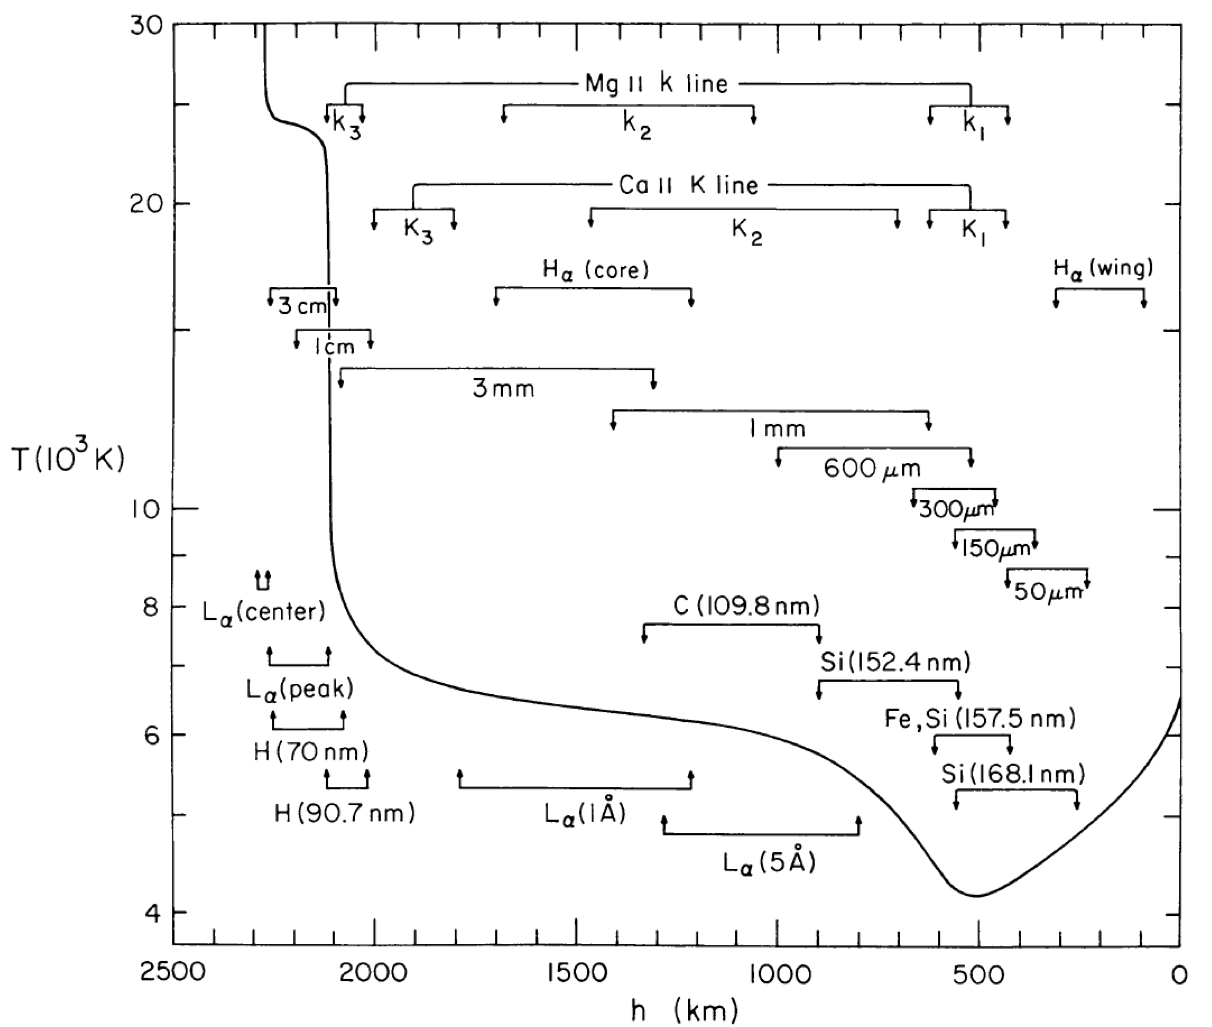
\includegraphics[width=0.95\linewidth]{figs/fig8}
	\caption{一些色球谱线和它们对应的形成高度。来源:\textcite{Vernazza1981}}
	\label{fig:8}
	\end{minipage}%
	\hfill
	\begin{minipage}[t]{0.5\linewidth}
	\centering
	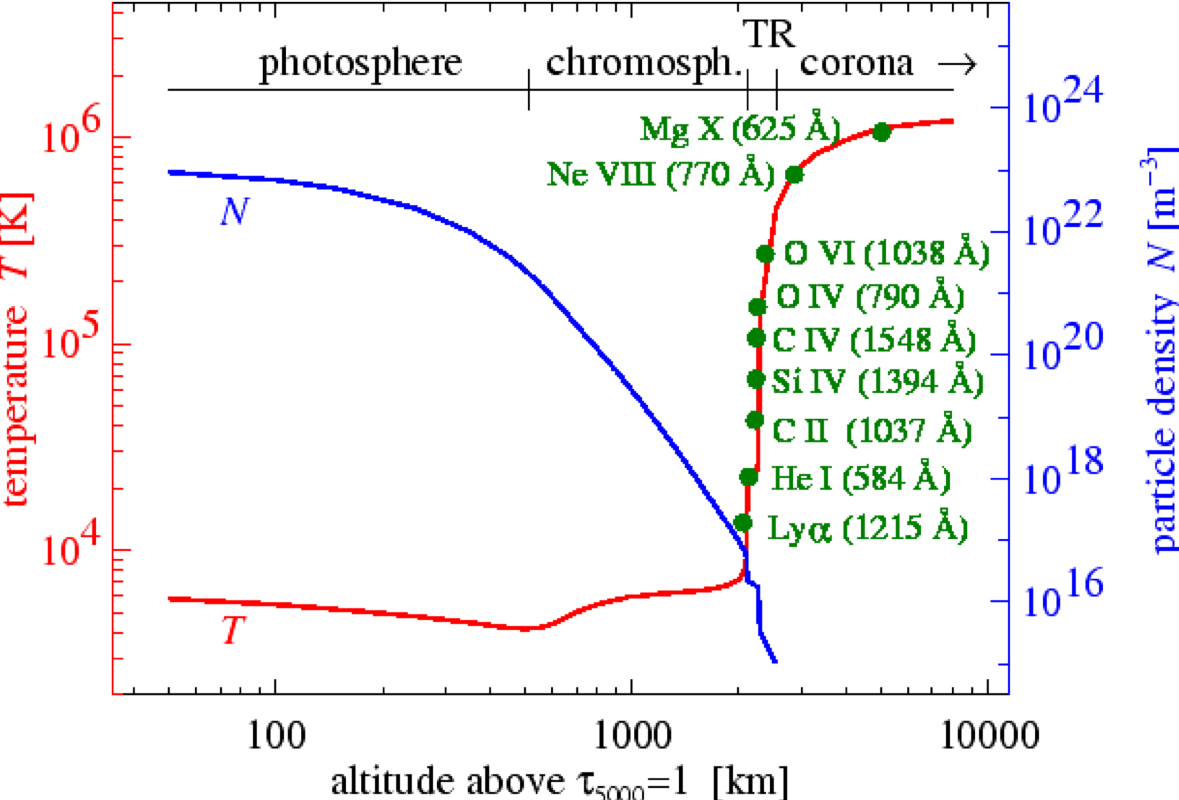
\includegraphics[width=0.95\linewidth]{figs/fig9}
	\caption{部分过渡区谱线和对应的形成高度。来源:\textcite{Peter2004}}
	\label{fig:9}
	\end{minipage}
\end{figure}
\subsection{Mg \textsc{ii}线}
Mg \textsc{ii}离子形成的发射/吸收线在UV波段较为明显的是Mg \textsc{ii} h, k和三重线。Mg \textsc{ii} h和k 线($\lambda_h = 2803.53~\mbox{\AA}, \lambda_k = 2796.35~\mbox{\AA}$,注意:在这篇文章中所有紫外谱线的波长都是真空波长)是太阳色球光谱中最明显的两条发射线之一。它们是Mg \textsc{ii}原子第一激发态到基态跃迁的共振线,由于第一激发态精细结构能级劈裂而分裂成两条,对应上下能级分别为从$3p\ ^2\mathrm{P}_{1/2}$到$3s\ ^2\mathrm{S}_{1/2}$和从$3p\ ^2\mathrm{P}_{3/2}$到$3s\ ^2\mathrm{S}_{1/2}$能级。在h和k线波长附近,还有另外三条谱线($\lambda = 2791.60~\mbox{\AA},\ 2798.75~\mbox{\AA}$ 和 $2798.82~\mbox{\AA}$),它们被称为三重线。在本文中波长较短的被称作Mg \textsc{ii} 2791线,而另外两条重叠的波长较长的线被称作Mg \textsc{ii} 2798线。它们来自于Mg \textsc{ii}第二激发态到第一激发态的跃迁,对应的能级分别为从$3d\ ^2\mathrm{D}_{3/2}$到$3p\ ^2\mathrm{P}_{1/2}$, $3d\ ^2\mathrm{D}_{3/2}$到$3p\ ^2\mathrm{P}_{3/2}$和从$3d\ ^2\mathrm{D}_{5/2}$到$3p\ ^2\mathrm{P}_{3/2}$。由于这些谱线都位于NUV波段,因此只能在离开地面足够高的高度进行观测。一些早期对宁静太阳上Mg \textsc{ii} h和k线的观测都显示了它们具有线心反转(\textit{central reversal})的结构\parencite{Lemaire1967,Lemaire1969,Doschek1977},而在耀斑带上则没有这样的结构,是一条纯发射线\parencite{Kohl1976K,Feldman1977}。一些辐射转移模拟也证明Mg \textsc{ii} h和k线的线心形成在高色球,而线翼则形成在低色球和温度极小区附近\parencite{Vernazza1981},见图~\ref{fig:8}。同时在NLTE的辐射转移模拟中,PRD效应被认为对Mg \textsc{ii} h和k线的形成起了重要作用,同时谱线的线心反转来自于线心形成与NLTE情况下,线心源函数在形成高度以下已经和Planck函数脱耦\parencite{Milkey1974,Ayres1976,Uitenbroek1997}。

在IRIS卫星发射前,针对其能观测到的一系列重要谱线(包括Mg \textsc{ii})在宁静太阳和谱斑等区域的谱线轮廓与形成高度进行了一系列的三维辐射磁流体力学模拟。在这一系列模拟中,再次确认了PRD效应对Mg \textsc{ii}谱线形成的重要性,且发现三维辐射转移对Mg \textsc{ii} h和k线的线心形成有比较重要的影响\parencites{Leenaarts2013a}。\textcites{Leenaarts2013b}进一步指出可以把Mg \textsc{ii} h和k线作为诊断太阳高层色球大气速度和温度的重要工具。\textcites{Pereira2015}研究了Mg \textsc{ii}三重线模拟中的谱线特征,他们发现大多数情况下Mg \textsc{ii}三重线形成与低色球并且是吸收线。但当低色球被加热时,Mg \textsc{ii}三重线会从吸收线转变为发射线,其线心线翼强度比可以用来推断低色球温度升高程度。

IRIS卫星发射后,观测到了一系列在耀斑带上轮廓出现明显变化的Mg \textsc{ii}线。Mg \textsc{ii} h,k包括三重线一般都显现出无线心反转的发射特征(见图\ref{fig:3})\parencites{Tian2015,Kerr2015,Tian2018}。Mg \textsc{ii} h和k线一般展现出较小的红翼不对称性和一个大约为十几$ \mathrm{km}\ \mathrm{s^{-1}}$的红移\parencites{Li2015,Li2017,Tian2018}。在一些比较大的耀斑中,IRIS卫星还在耀斑带的前缘发现了一些存在中心反转,但有着强烈红翼增强的Mg \textsc{ii} h和k线\parencites{Liu2015,Panos2018}。在某些耀斑爆发的初期,还观测到了一部分蓝翼增强的Mg \textsc{ii} h和k线,可能来自于一部分较冷物质$\sim10^4$ K在色球蒸发初期的上流\parencites{Tei2018}。

这些在宁静太阳上难以观测到的Mg \textsc{ii}谱线特征激发了新一轮的辐射流体力学模拟的兴趣,由于耀斑过程中的色球动力学过程非常复杂,这些模拟目前还只是在使用一维辐射流体力学代码(RADYN: \cites{Allred2005,Allred2015}; \cites{Carlsson1992,Carlsson1997}; RH: \cites{Uitenbroek2001}; \cites{Pereira2015b})进行计算。\textcites{Rubio2016}对2014年3月29日的X1.1级耀斑进行了模拟,他们发现耀斑带上的Mg \textsc{ii}线在模拟中仍然处于线心反转并且与观测相比显得非常窄。之后的一个参数研究工作通过人为提高Mg \textsc{ii}线心形成位置附近的电子密度一个量级,以保持LTE条件,在观测上再现了Mg \textsc{ii}非线心反转的谱线特征。但是这些合成的(\textit{synthetic})谱线仍然不够宽\parencites{Rubio2017}。同时\textcites{Rubio2017}提出一些剧烈增宽的非对称的谱线可以通过两个在观测上没有分辨的速度达到约$250\ \mathrm{km}\ \mathrm{s^{-1}}$速度上下流造成的红蓝移谱线叠加而成。另外一些通过对模拟得到的Mg \textsc{ii}谱线在时间上进行叠加的“多环”(\textit{multi-thread})模拟也能够部分再现Mg \textsc{ii}谱线的致宽和解释Doppler频移变化\parencites{Reep2019}。\textcites{Kerr2016}用Alfv\'en波加热低层大气来模拟耀斑能量释放,他们发现Mg \textsc{ii} h和k线逐渐由线心反转变为非线心反转,但谱线的红翼不对称性和致宽特征并没有得到很好的再现。


\subsection{Si \textsc{iv}线}
位于太阳光谱FUV波段的Si \textsc{iv}双重线($\lambda = 1393.755~\mbox{\AA}, 1402.770~\mbox{\AA}$)是Si \textsc{iv}的基态到第一激发态跃迁产生的两条共振线,由于原子能级精细结构分裂而形成两条线,对应的能级分别是从$2p^63s\ ^2\mathrm{S}_{1/2}$到$2p^63p\ ^2\mathrm{P}_{3/2}$与$2p^63s\ ^2\mathrm{S}_{1/2}$到$2p^63p\ ^2\mathrm{P}_{1/2}$。这两条线在70-80年代也在各类恒星,乃至类星体的光谱中被观测到\parencites{Stalio1975,Imhoff1980,Saxner1981,Oranje1982}。由于Si \textsc{iv}离子较高的电离态,其一般被认为是在过渡区温度约为$8\times10^4$ K处形成\parencites{Jordan1969,Doschek1997}。在太阳上对Si \textsc{iv}线的观测最早来自于\textcites{Brueckner1972,Brueckner1973}。在70年代末,天空实验室(\textit{Skylab}),环绕太阳天文台8(\textit{Orbiting Solar Observatory 8, OSO-8})和太阳极大年任务(\textit{Solar Maximum Mission, SMM})上搭载的光谱仪对宁静太阳\parencites{Doschek1976,Mariska1978,Shine1976}、冕洞\parencites{Feldman1976,Francis1977}、网状结构\parencites{Feldman1976b}和耀斑带上\parencites{Porter1984}等位置的Si \textsc{iv}线和其它紫外谱线分别从日面和临边角度进行了大量观测。由于一般认为它们在日面上是光学薄的(两条线发射强度比为2:1),且谱线形状能较好得被单Gaussian形的谱线拟合,所以被大量运用在测量运动速度\parencites{Feldman1976,Gebbie1981},湍动速度\parencites{Feldman1977c},建立过渡区模型\parencites{Roussel-Dupre1981}等研究。在临边高出2-4个角秒以上,Si \textsc{iv}的光学深度会明显增加,但通过一些简单的辐射转移近似也可以用来研究过渡区中的物质流动\parencites{Roussel-Dupre1979,Doschek1981}。

IRIS卫星发射后,Si \textsc{iv}线的观测又迎来了一个新的爆发式发展的时代。特别是针对一系列耀斑带的观测,Si \textsc{iv}线作为过渡区的重要发射线几乎在所有的耀斑观测中都得到了分析。在耀斑带上,Si \textsc{iv}往往展现出复杂的谱线形状。在一些耀斑中,Si \textsc{iv}仅出现强烈的红翼增强,但没有完全红移\parencites{Tian2014,Tian2015,Tian2018,Brosius2015,Polito2016},其中有一些谱线轮廓可以被一个红移较小的Gauss分量和另一个红移较大的Gauss分量拟合\parencites{Li2015,Lee2017}。而在另一些耀斑中,Si \textsc{iv}谱线又展现出一个整体红移约为$\sim50\ \mathrm{km}\ \mathrm{s^{-1}}$的单Gaussian形分量\parencites{LiD2017,Li2017},这可能来自于非热电子或热传导加热低层大气的高度和程度差异\parencites{Li2017}。和Mg \textsc{ii} h和k线的演化相比,这些红移/红翼不对称性一般会持续较长的时间\parencites{Warren2016},同时可能伴随着一个周期为0.5-6分钟的亮度准周期性振荡(\textit{quasi-periodic fluctuation}, \cites{Brosius2015,Zhang2016,Tian2018}),可能来自于日冕中的多次的重联过程\parencites{Brosius2015}。整个谱线的红移/红翼不对称性被普遍认为是存在较冷物质向下运动的重要证据,但对于其具体机制还存在着不同解释:\textcites{Reep2016}和~\textcites{Warren2016}认为其来自于多个耀斑环的持续的辐射冷却的叠加;\textcites{Tian2015}和~\textcites{Brannon2016}认为其来自于冷却的物质下流,还有认为其来自于较长的低层大气能量释放时间\parencites{Li2017}。

对耀斑带上Si \textsc{iv}谱线的辐射转移模拟较少,原因在于一般认为其是光学薄的,因此可以直接使用CHIANTI\parencites{Dere1997,Landi2013}等原子数据库进行计算。在耀斑带上观测到的明显的红翼不对称的谱线预示着Si \textsc{iv}线可能在耀斑带上存在光学厚的情况,需要细致的辐射转移计算。\textcites{Reep2016}在模拟中通过多个耀斑环叠加再现了Si \textsc{iv}谱线在耀斑带上的持续红移。\textcites{Kerr2019}利用RADYN代码对其进行了详细的辐射转移模拟,发现在较高非热电子能量加热($E>10^{10}\ \mathrm{erg}\ \mathrm{cm^{-2}s^{-1}}$)的耀斑中,形成于$3\times10^4-6\times10^4$ K间的Si \textsc{iv}线表现出光学厚的特征;而在较小的耀斑中($E<10^{10}\ \mathrm{erg}\ \mathrm{cm^{-2}s^{-1}}$),形成于$8\times10^4-10^5$ K间的Si \textsc{iv}线表现出光学薄的特征。
\subsection{C \textsc{ii}线}
在太阳FUV光谱中C \textsc{ii}线指在1335 \mbox{\AA}附近的三条谱线,是C \textsc{ii}离子第一激发态到基态的共振线,由于能级精细结构分裂成三条线($\lambda = 1334.532~\mbox{\AA}, 1335.663~\mbox{\AA}, 1335.708~\mbox{\AA}$),其中1335 \mbox{\AA}两条谱线由于波长相近而重叠在一起。它们对应的能级跃迁分别是从$2s^22p$ $^2\mathrm{P}_{1/2}$到$2s2p^2\ ^2\mathrm{D}_{3/2}$,$2s^22p\ ^2\mathrm{P}_{3/2}$到$2s2p^2\ ^2\mathrm{D}_{3/2}$与$2s^22p\ ^2\mathrm{P}_{3/2}$到$2s2p^2\ ^2\mathrm{D}_{5/2}$。\textcites{Detwiler1961}最早在太阳上观测到了FUV的C \textsc{ii}线,其谱线轮廓也在不久之后得到了准确的测量\parencites{Berger1970}。同时C \textsc{ii}线也在一系列的恒星中被观测到\parencites{Freire1979,Praderie1980,Kamp1982}。基于这些观测,\textcites{Berger1970}进行了一些基于统计平衡和NLTE的辐射转移计算,发现拟合较好的C \textsc{ii}线形成在$15000-20500$ K,宽度在$60-160$ Km的区域内。OSO-8卫星也对C \textsc{ii}谱线进行了一系列观测,其被发现对大气模型中的20000 K温度平台非常敏感\parencites{Lites1978},也被用于观测色球中波的传播\parencites{Chipman1978}。进一步的研究表明,活动区上的C \textsc{ii}总强度与活动区总磁通量有比较好的关系,可能是活动区中的磁力线对色球和日冕加热产生贡献导致的\parencites{Schrijver1987}。在耀斑发生时,C \textsc{ii}线强度也会剧烈增强,是FUV波段的连续谱的主要贡献之一\parencites{Doyle1992,Brekke1996}。

IRIS卫星的发射重新点燃了太阳物理学界对C \textsc{ii}线光谱诊断的兴趣。Rathore等人在2015年利用Bifrost三维辐射流体力学模拟的结果,深入探讨了各种因素对C \textsc{ii}在宁静太阳和谱斑区域的谱线形成的影响以及C \textsc{ii}作为光谱诊断工具的能力\parencites{Rathore2015a,Rathore2015b,Rathore2015c}。他们得到的结果包括:1)PRD效应对C \textsc{ii}谱线轮廓影响不大,但三维辐射转移效应对C \textsc{ii}线心形成起着重要作用。2)C \textsc{ii}线心大致形成在$6\times10^3-2.5\times10^4$ K间,对应的柱密度约为$10^6\ \mathrm{g}\ \mathrm{cm^{-2}}$的区域内。线心贡献函数最大处高度和过渡区高度(温度高于$3\times10^{4}$ K的最高高度)有非常好的相关性。3)光学深度对C \textsc{ii}谱线轮廓起着非常重要的作用,包括进一步致宽谱线和两条线的强度比。因此光谱诊断反演必须基于光学厚的辐射转移才能得到正确的结果。4)C \textsc{ii}线心在模拟中会存在单发射峰和线心反转(双峰)两种情况,线心反转谱线两个峰的不对称性和线心附近的大气速度梯度有关。5)谱线的Doppler频移能够比较好的反映线心形成高度的速度场。6)和形成在约为$8\times10^4$ K的Si \textsc{iv}线相比,C \textsc{ii}线和Mg \textsc{ii}线类似,都形成在相对较低的高度。C \textsc{ii}和Mg \textsc{ii}谱线的形成位置相对高低主要由$1.4\times10^4-5\times10^4$ K间物质密度分布决定。和IRIS观测到的谱线相比,他们的模拟也存在着一系列问题。其一是观测中的C \textsc{ii}线更宽,其半高全宽大约是模拟中的2倍;其二是模拟中的谱线大多是单发射峰,但观测上发现了大量的线心反转谱线,预示着C \textsc{ii}线心源函数在形成高度处也已经和Planck函数脱耦;其三是观测中C \textsc{ii}两线强度比(约为1.1-1.2)比模拟中得到的强度比(约1.4-1.7)要小。

在耀斑带上的C \textsc{ii}谱线也表现出类似于Mg \textsc{ii}和Si \textsc{iv}的轮廓结构,从有线心反转的谱线向单发射线转化,强度大约增强1-2个量级,谱线变宽,同时表现出一定的红翼不对称性\parencites{Li2015,Li2017}。C \textsc{ii}线的红移与Si \textsc{iv}线类似\parencites{Brosius2017},能够持续10分钟甚至更长的时间\parencites{Li2017}。在时间顺序上,C \textsc{ii}的红翼的增强出现于耀斑爆发相之前\parencites{Sadykov2015},也在IRIS能够观测到的高温谱线Fe XXI线在色球蒸发中出现明显蓝移之前\parencites{Brosius2018}。同时其红移大小在时间上与RHESSI卫星观测到的硬X射线12-25 KeV流量大小也有比较好的相关性\parencites{Sadykov2016}。在空间位置上,C \textsc{ii}的红移一开始也出现在耀斑带前缘\parencites{Battaglia2015},证明其与耀斑爆发中的非热电子入射或热传导有着比较强的关系。和Si \textsc{iv}线类似,耀斑带上的C \textsc{ii}线亮度也会产生准周期性的振荡\parencites{Brosius2015,Brosius2018},且其谱线宽度也会随着强度发生振荡\parencites{Warren2016}。此外在\textcites{Tei2018}中出现蓝移的Mg \textsc{ii}线位置上,C \textsc{ii}也展现了比较复杂的谱线轮廓,存在一个静止的存在线心反转的分量和一个比较强的红翼增强和不对称性。

\section{研究动机}
基于以上的研究我们可以看到,形成于色球和过渡区的紫外谱线对太阳以及M矮星上的各种各样的爆发活动均有不同程度的响应,为我们提供了获取这些爆发活动对应的色球和过渡区的动力学过程的重要诊断方法。但由于这些谱线大多形成在光学厚的区域,需要进行辐射转移的模拟才能理解其特征谱线轮廓对应的特定大气参数随高度的分布。在这篇论文中,我们将尝试使用已有的RADYN和RH代码,对这些不同的爆发时间都进行一定程度的研究。一方面我们希望检验这些代码在模拟这些不同尺度的爆发过程中的可用性和可靠性;另一方面我们也希望能够通过这些模拟帮助研究人员更好地理解在爆发过程中出现的特殊谱线轮廓究竟来自于哪些可能的物理过程。

% vim:ts=4:sw=4

	% Copyright (c) 2014,2016 Casper Ti. Vector
% Public domain.

\chapter{研究方法概述}\label{chap:2}
\section{RADYN代码}
我们采用了一维辐射流体力学模拟代码RADYN\parencite{Carlsson1992,Carlsson1997,Allred2005,Allred2015}来模拟低层大气在沿耀斑环向下传播的非热电子加热时的动力学演化过程。RADYN代码是由挪威奥斯陆大学(\textit{University of Oslo})的Mats Carlsson教授于上世纪90年代开发的流体力学代码,其最主要的特点是能够考虑非局部热动平衡和非平衡电离下的辐射转移过程。最早它被运用于研究在明亮米粒组织结构是如何被低层激波加热的,成功再现了米粒组织上的Ca \textsc{ii} H和K线的Doppler频移震荡现象\parencites{Carlsson1997}。90年代末美国华盛顿大学(\textit{University of Washington})的Suzanne L. Hawley教授意识到了其在模拟耀斑等剧烈的大气动力学过程中的潜力,并和其他研究者合作将其开发为能够模拟非热电子加热低层大气的辐射流体力学代码。\textcites{Abbett1999}率先在RADYN代码中加入了非热电子加热,软X射线加热以及来自于轫制辐射和金属碰撞激发造成的光学薄辐射冷却等过程,对耀斑的爆发相进行了模拟。\textcites{Allred2005}拓展了代码的应用范围,使其同样可以用于模拟M矮星上同样由非热电子作为低层大气加热机制的耀斑。随后RADYN代码又新增了Fokker-Planck方程来计算非热电子加热,非热电子撞击硬靶(\textit{thick target})产生返回电流对日冕的加热\parencites{Allred2015},更加精确的Balmer线系线性Stark效应的致宽\parencites{Kowalski2017b}等一系列新的特征,对耀斑爆发过程进行了更加细致的模拟。下面我们对主要的物理过程及其数值处理方法做一个简介,涉及代码内部计算的公式全部引自\textcites{Allred2015}。

\subsection{流体力学及辐射转移方程组}
RADYN代码采用求解一维流体力学及辐射转移方程组的方法来模拟太阳耀斑爆发时低层大气的动力学演化。其主要方程组如下\parencites{Allred2015}:

\begin{gather}
	\frac{\partial \rho}{\partial t}+\frac{\partial \rho v}{\partial z}=0 \\
	\frac{\partial \rho v}{\partial t}+\frac{\partial \rho v^{2}}{\partial z}+\frac{\partial\left(p+q_{\mathrm{v}}\right)}{\partial z}+\rho g-A_{\mathrm{beam}}=0  \\
	\frac{\partial \rho e}{\partial t} +\frac{\partial \rho v e}{\partial z}+\left(p+q_{\mathrm{v}}\right) \frac{\partial v}{\partial z} +\frac{\partial\left(F_{\mathrm{c}}+F_{\mathrm{r}}\right)}{\partial z}-Q_{\mathrm{cor}}-Q_{\mathrm{beam}}-Q_{\mathrm{rc}}=0 \\
	\frac{\partial n_{i}}{\partial t}+\frac{\partial n_{i} v}{\partial z}-\left(\sum_{j \neq i}^{N^{\prime}} n_{j} P_{j i}-n_{i} \sum_{j \neq i}^{N^{\prime}} P_{i j}\right)=0 \\
	\mu \frac{\partial \boldsymbol{I}_{\nu \mu}}{\partial z}=\eta_{\nu \mu}-\chi_{\nu \mu} \boldsymbol{I}_{\nu \mu}
\end{gather}
其中,$z$, $e$, $\rho$, $v$和$p$分别代表高度、内能密度,密度,一维速度和压强。$g$是重力加速度,$q_v$是粘性项。$F_c$为对流热流,$F_r$为辐射通量。$P_{ij}$是能级$i$到$j$之间的跃迁频率,包含了碰撞跃迁频率$C_{ij}$与辐射跃迁频率$R_{ij}$。辐射转移方程为一维平面平行层形式,能量方程中的辐射通量$F_r$由$\boldsymbol{I}_{\nu\mu}$在立体角上积分得到。$Q_{cor}$是一个人工的日冕加热项。$Q_{\mathrm{beam}}$和$A_{\mathrm{beam}}$是由于入射入射非热电子带来的能量和动量。

\subsection{光学厚与光学薄辐射转移}
对于光学厚的辐射转移,RADYN会详细计算部分原子部分能级的NLTE下的能级平衡和辐射转移方程。这些原子包括一个6能级的氢原子模型,一个9能级的氦原子模型,一个6能级的Ca \textsc{ii}离子模型和一个4能级的Mg \textsc{ii}原子模型。剩下原子造成的不透明度将会采用\textcites{Gustafsson1973}的代码在LTE的假设下处理,给出一个依赖于温度、密度和频率的不透明度函数。对于日冕中不同温度成分的光学薄辐射造成的能量损失,由CHIANTI原子数据库\parencites{Dere1997,Landi2013}计算得出。
\subsection{加热机制}
这里主要介绍模型中三种主要的加热机制和它们的处理方法:

\textbf{非热电子束加热}\ \ RADYN代码考虑了相对论效应,Coulomb碰撞,回旋同步辐射,投掷角散射和磁场梯度效应,采用一个Fokker-Planck方程来描述非热电子的能量分布函数$f(E,\mu,z)$\parencites{Allred2015}
\begin{multline}
	\mu \frac{\partial \Phi}{\partial z}-\frac{d \ln B}{2 d z} \frac{\partial}{\partial \mu}\left[\left(1-\mu^{2}\right) \Phi\right] =\frac{1}{\beta^{2}} \frac{\partial}{\partial E}\left\{\left[C+S \beta^{3} \gamma^{2}\left(1-\mu^{2}\right)\right] \Phi\right\} \\
	-\frac{S}{\beta \gamma} \frac{\partial}{\partial \mu}\left[\mu\left(1-\mu^{2}\right) \Phi\right] +\frac{C^{\prime}}{\beta^{4} \gamma^{2}} \frac{\partial}{\partial \mu}\left[\left(1-\mu^{2}\right) \frac{\partial \Phi}{\partial \mu}\right]+\frac{\Sigma}{c \beta^{2}}
\end{multline}
其中,$\beta$为离子的相对论因子,$\Phi = f/\beta $,$\gamma = E+1$是无量纲化的相对论性总能量。$\Sigma$是电子从环顶入射的源项,$C$与$C'$是描述电子能量损失和投掷角扩散的因子,$S$是用来描述电子同步回旋辐射能量散失的因子。这些参数的具体形式参见\textcites{Allred2015}。RADYN代码将计算在电子和带电粒子、中性粒子相互作用散失能量时的分布函数变化,同时给出非热电子对局部大气的加热。

\textbf{XEUV逆加热(EUV backwarming)}\ \ 由于耀斑过程中会产生低层大气中的X射线和EUV辐射,这些高能光子同样也会重新通过光致电离等过程重新加热低层大气。这些加热在RADYN代码中都依靠CHIANTI原子数据库给出的发射系数确定。

\textbf{返回电流加热(return current heating)}\ \ 显然当一系列非热电子沿耀斑环向下传播时会形成一个向上的宏观电流,这个电流同样会贡献出焦耳加热项。在同时考虑入射电子热和非热成分后,RADYN代码采用如下公式来计算返回电流加热\parencites{Allred2015}:
\begin{equation}
	Q_{\mathrm{rc}}(x)=\begin{cases}\eta e^{2} F_{\mathrm{e}}^{2} & x<x_{rc} \\ {\eta e^{2} F_{\mathrm{e}}^{2}\left(\delta \frac{E_{\text { therm }}}{E_{\mathrm{c}}}+\frac{V(x)}{E_{\mathrm{c}}}\right)} \\ { \times\left(\frac{E_{\text { therm }}}{E_{\mathrm{c}}}+\frac{V(x)}{E_{\mathrm{c}}}\right)^{1-2 \delta}} &x\geq x_{rc} \end{cases} 
\end{equation}
其中$\eta$是电阻率,$F_e$是电子束通量,$\delta$是非热电子分布谱指数,$E_c$是非热电子截止能量。$x$为据环顶的距离,$x_{rc}$是电子被完全热化时距环顶的距离。一般来说,返回电流会让非热电子束在日冕中耗散更多的能量。
\subsection{初始输入}\label{sec:2.1.4}
在运行RADYN代码时,主要调节的参数是入射非热电子束的参数和初始大气条件。下面主要介绍的是比较重要的参数:

\textbf{电子束参数}\ \ RADYN输入中要求提供程序运行各时间点从环顶入射的非热电子束的参数,一般包括非热部分的谱指数$\delta$,截止能量$E_c$与总能量通量。一般来说,更大的截止能量$E_c$会让电子束在更深的大气中耗散大部分能量。而更大的谱指数(谱更加硬了)$\delta$会让电子束在低层大气中有更大的加热率。一般来说截止能量$E_c$设置在几十KeV,而谱指数$\delta$一般在3-6左右,能量通量根据模拟耀斑的等级不同而不同,对于太阳耀斑一般在$10^8-10^{12}\ \mathrm{erg\  cm^{-2}\  s^{-1}}$左右。

\textbf{初始大气}\ \ 
为了模拟一维耀斑环在电子束入射之前的初始大气状态,RADYN提供了一系列的初始大气。一般来说初始大气包含几个特征参数:光球层温度、耀斑环长度、日冕电子密度和日冕温度。光球层温度一般在$5000-5800$ K,耀斑环长度在$10-100$ Mm之间,日冕电子密度一般在$10^8\ \mathrm{cm^{-3}}$量级,日冕温度在MK量级。此外,RADYN还提供了一个M矮星的初始大气用于恒星耀斑的模拟,其拥有较低的光球层温度($\sim 3500$ K)和较高的日冕电子密度($10^{10}\ \mathrm{cm^{-3}}$)和温度。
\section{RH代码}
RH代码\parencites{Uitenbroek2001}是一套利用基于多能级加速$\Lambda$迭代(\textit{multi-level accelerated lambda iteration, MALI})方法计算给定大气中NLTE辐射转移过程的代码。整套方法基于\textcites{Rybicki1991},但考虑了PRD效应的影响。在这篇文章中,我将使用RH代码的MPI版本,RH1.5D代码\parencites{Pereira2015b}来求解耀斑大气中的辐射转移过程。RH1.5D代码支持并行计算多个一维大气模型中的辐射转移过程,能够大大加快计算速度。同时,RH1.5D代码还支持使用\textcites{Leenaarts2012}中描述的散射过程中各向异性PRD的近似算法,对模拟Mg \textsc{ii}等一系列由散射形成的谱线能得到比较好的结果。RH代码的一个缺点是假设辐射转移过程中原子能级占据数是统计平衡假设下的,即能级粒子数不随时间变化,这在耀斑这样剧烈爆发的模拟中可能并不是很好的假设\parencites{Abbett1999,Rubio2017}。

\subsection{求解过程}
限于篇幅和作者能力有限,我们在此不再详细叙述RH内部计算辐射转移过程的具体公式,仅对整个迭代求解过程做一个简单介绍。首先,代码将建立所有计算波长点和跃迁能级的列表;之后将建立一个能级上粒子数分布的初始解,可以是基于LTE情况下的,也可以是基于无辐射场情况下的;之后基于给定的原子能级数和一个给定的发射吸收谱线强度比$\rho$,计算出在PRD情况下的辐射场参数;之后在基于固定的原子能级数的情况下,重新计算发射吸收谱线强度比$\rho$。最后这两步可以持续迭代,直到前后两步得到的平均辐射强度的相对差异小于设定的阈值。

\subsection{输入输出}
接下来我们简单介绍一下RH1.5D代码支持的输入和输出参数。为了让代码能够正常运行,需要输入的大气参数是:(一维)温度分布,电子密度分布,氢原子能级粒子数分布,宏观速度分布,微观湍动速度分布和各个格点的高度。如果需要计算Stokes参数,还需要给出磁感应强度矢量的分布。同时可以在\texttt{atoms.input} 文件中输入文件中指定在模拟中使用的原子,跃迁能级和是否当作LTE背景不透明度处理。在\texttt{ray.input}文件中可以指定求解辐射转移方程的方位角$\mu$和需要详细输出辐射转移波长的波长点。在\texttt{keyword.input}文件中还有一系列代码选项,如收敛阈值、是否使用大气波长、是否输出$\tau=1$的高度,是否需要去除某个温度以上的所有大气方便计算和是否计算Stokes参量等可供修改。在输出文件中,主要包含了辐射强度$I_{\nu}$,各原子能级粒子数等,如果使用了Stokes模式,还会有$UVQ$等一系列参量,如果在\texttt{ray.input}中指定了波长点,还可以输出这些波长点的不透明度$\chi_\nu$和源函数$S_\nu$等与辐射场有关的参量。
\subsection{Stark致宽效应处理}\label{sec:2.2.3}
为了呼应后面介绍的Stark-B数据库,我们在这里简单介绍一下RH代码中对于非氢原子的二次Stark效应致宽的计算方法。计算Stark致宽效应的经典方法主要有两种,一种是碰撞理论(\textit{impact theory},\cites{Weisskopf1932}),另一种是统计理论(\textit{statistical theory},\cites{Holtsmark1919})。前者的物理图像是每次与带电粒子的碰撞会打断辐射粒子的辐射,经过Fourier变换后非无穷长的波列将会在频域空间有一定的展宽,最后将会得到一个Lorentzian形的谱线。而后者则同时考虑多个带电粒子在辐射粒子周围的统计分布,在带电粒子和辐射粒子相对静止的假设下,计算他们的电场对辐射粒子能级的扰动,最后会得到一个Holtsmark分布。一般来说,对于自由电子的Stark致宽而言,碰撞理论能够得到比较好的结果,对于一条较宽的谱线而言,在线心周围碰撞效应的近似比较好,而在线翼部分统计理论的效果比较好,关于这两种经典方法的优劣,可以参见附录\ref{sec:a.2}中对于Mg \textsc{ii}线的讨论。

RH代码采用Lindholm近似\parencites{Lindholm1945,Foley1946,Mihalas2014}下的经典碰撞理论来计算非氢原子的二次Stark效应致宽,其给出Lorentzian形谱线的半高全宽$\Gamma_{Stark}$为
\begin{equation}
    \Gamma_{Stark}=11.37C_4^{2/3}v_{rel}N_e
\end{equation}
其中$v_{rel}$为辐射粒子和带电粒子的相对速度,$N_e$为电子密度,$C_4$为Stark常数,用于衡量当一个带电粒子在距离为$r$处与辐射粒子产生作用时辐射粒子的辐射角频率改变量大小$\Delta \omega = C_4/r^4$。在RH代码中,其通过\textcites{Traving1960}中的如下公式进行计算
\begin{equation}
    C_4 = \frac{e^2 r_{bohr}^3}{4 \pi \epsilon_0 \hbar}\  \frac {\left(n_{\mathrm{effu}} \  \left(5.0  n_{\mathrm{effu}}^2 + 1.0\right)\right)^2 - \left(n_{\mathrm{effl}} \  \left(5.0  n_{\mathrm{effl}}^2 + 1.0\right)\right)^2}{18.0 \  Z^4}    
\end{equation}
其中
\begin{align}
	n_{\mathrm{effl}} &=Z \sqrt{R_{\mu} /\left(E_{c}-E_{i}\right)} \\
	n_{\mathrm{effu}} &=Z \sqrt{R_{\mu} /\left(E_{c}-E_{j}\right)}
\end{align}
$E_c$为该电离态原子的电离能,$E_i$为跃迁的低能级能量,$E_j$时该跃迁的高能级能量,$Z$为等效电荷,$R_\mu$为Rydberg常数。
\section{STARK-B数据库}\label{sec:2.3}
STARK-B数据库\parencites{STARK-B}提供了大量天体物理中重要原子谱线在周围电子和离子扰动下的致宽宽度的数据。整个数据库旨在为恒星大气和包层(\textit{envelope})提供精确计算Stark致宽效应的数据。其中主要运用半经典碰撞理论\parencites{Brechot1969a,Brechot1969b,Fleurier1977,}来计算Stark致宽效应。其中包含了带电粒子的相互作用的双曲线轨道,粒子的偶极、四极相互作用,非弹性碰撞等。对于已经计算了的跃迁,其给出$\Gamma_{Stark}$在不同温度下的值,并提供了一个拟合函数供数值模拟使用\parencites{Brechot2011}:
\begin{equation}
    \log\left(\Gamma (\mbox{{\AA}})\right) = a_0 + a_1\mathrm{Log}(T) + a_2\mathrm{Log}^2(T) 
\end{equation}

\begin{table}
	\begin{tabular}{cccccc}
	\hline
    谱线 & 跃迁 & 波长($\mbox{{\AA}}$) & $a_0$ & $a_1$ & $a_2$ \\ 
 	\hline
    Mg \textsc{ii} h& $3p\ ^2\mathrm{P}_{1/2}-3s\ ^2\mathrm{S}_{1/2}$  & 2803.53 & \multirow{2}{*}{1.13807} &\multirow{2}{*}{-1.54913} & \multirow{2}{*}{0.13423}\\ 
    Mg \textsc{ii} k& $3p\ ^2\mathrm{P}_{3/2}-3s\ ^2\mathrm{S}_{1/2}$  & 2796.35\\ 
    \hline
    Mg \textsc{ii} 2791  & $3d\ ^2\mathrm{D}_{3/2}-3p\ ^2\mathrm{P}_{1/2}$ &2791.60& \multirow{3}{*}{1.36331}& \multirow{3}{*}{-1.62649} & \multirow{3}{*}{0.15218}\\ 
    \multirow{2}{*}{Mg \textsc{ii} 2798}  & $3d\ ^2\mathrm{D}_{3/2}-3p\ ^2\mathrm{P}_{3/2}$ &2798.75\\
     & $3d\ ^2\mathrm{D}_{5/2}-3p\ ^2\mathrm{P}_{3/2}$ & 2798.82 \\
     \hline
    Si \textsc{iv} 1394& $2p^63s\ ^2\mathrm{S}_{1/2}-2p^63p\ ^2\mathrm{P}_{3/2}$  & 1393.755 & \multirow{2}{*}{-3.89461} &\multirow{2}{*}{0.65393} & \multirow{2}{*}{-0.13588}\\ 
    Si \textsc{iv} 1402& $2p^63s\ ^2\mathrm{S}_{1/2}-2p^63p\ ^2\mathrm{P}_{1/2}$  & 1402.770\\ 
    \hline
\end{tabular}
    \caption{本文中使用的STARK-B数据库数据}\label{Table1}
\end{table}

\begin{figure}
	\centering
	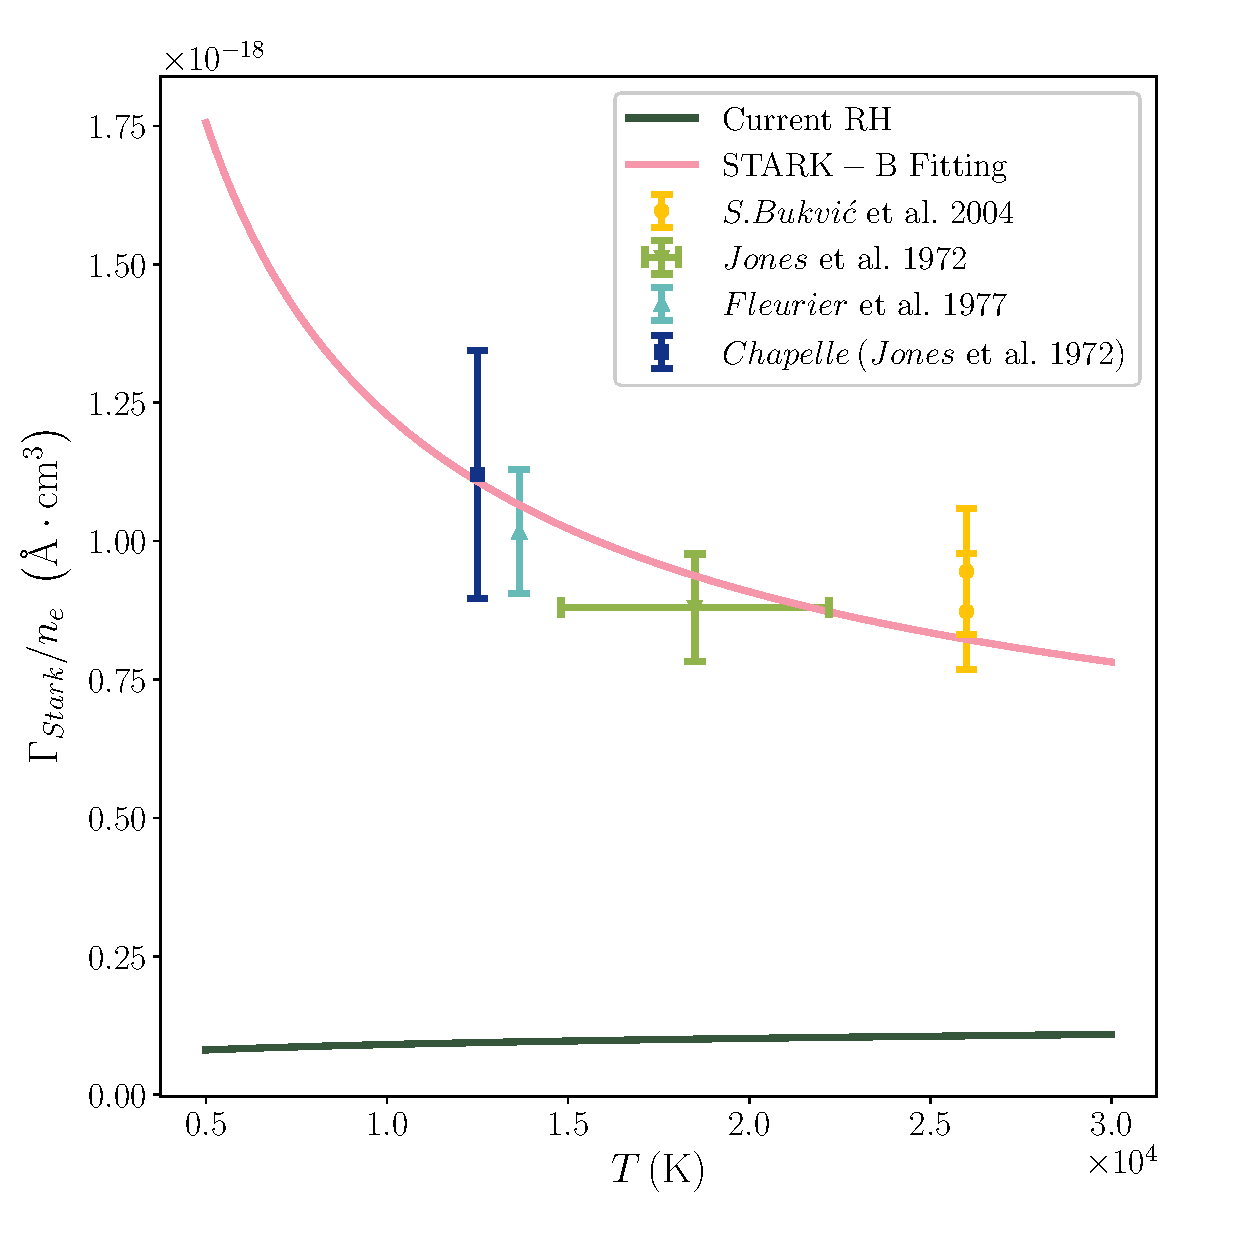
\includegraphics[width=0.6\textwidth]{figs/SB_Mg}
	\caption{RH代码与STARK-B数据库中对Mg \textsc{ii} h,k线的单位电子密度下Stark致宽宽度比较。同时我们还展示了一些实验得到的谱线致宽数据\parencites{Jones1972,Fleurier1977,Bukvic2004}。}\label{fig:2.1}
\end{figure}

\begin{figure}
	\centering
	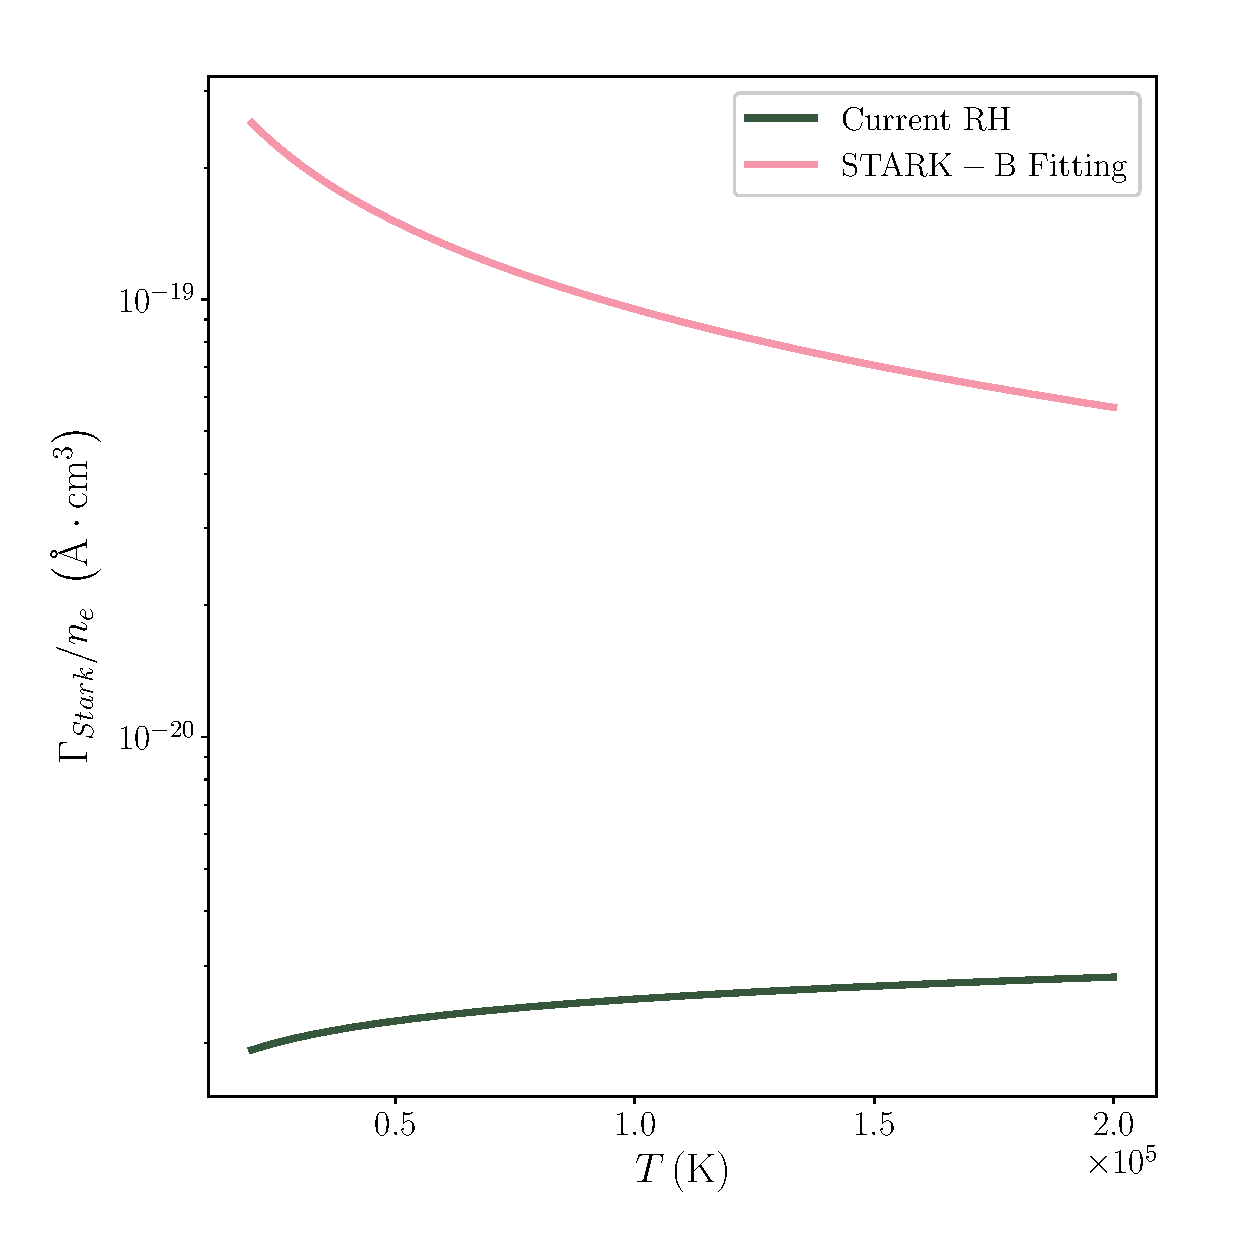
\includegraphics[width=0.6\textwidth]{figs/SB_Si}
	\caption{RH代码与STARK-B数据库中对Si \textsc{iv}双重线的单位电子密度下Stark致宽宽度比较。}\label{fig:2.2}
\end{figure}
表~\ref{Table1}给出了本文中使用的Mg \textsc{ii}和Si \textsc{iv}线的STARK-B数据库数据。我们比较了RH代码和STARK-B数据库对Mg \textsc{ii} h,k和三重线,以及Si \textsc{iv}双重线Stark致宽效应处理结果的不同。图~\ref{fig:2.1}展示了Mg \textsc{ii} h和k线的在单位电子密度下Stark宽度随温度的变化情况。总体上来看,STARK-B数据库给出的谱线宽度和实验结果拟合的比较好,同时比RH代码给出的结果大约高了一个量级。STARK-B数据库中的宽度随温度的增加而逐步降低(由非弹性碰撞向弹性碰撞变化),但RH代码中的结果随着温度的上升而缓慢增加(粒子相对速度提高的结果)。图~\ref{fig:2.2}展示了Si \textsc{iv}双重线的结果,可以看到RH代码同样大大低估了Si \textsc{iv}双重线的Stark致宽宽度,且其对温度的依赖关系也与STARK-B数据库的数据相反。但是由于Si \textsc{iv}线的Stark宽度本来就比Mg \textsc{ii}线低大约一个量级,且在Si \textsc{iv}形成高度上电子密度也相对较低,因此其Stark致宽相对于Mg \textsc{ii}线来说应该较不明显。
% vim:ts=4:sw=4
	% Copyright (c) 2014,2016 Casper Ti. Vector
% Public domain.

\chapter{事件研究:2014年3月29日耀斑}\label{chap:3}
在这一章节中,我们主要讨论对2014年3月29日太阳上爆发的一个X1.1级耀斑色球辐射的辐射流体力学模拟的结果。我们利用RADYN和RH代码,基于拉马第高能太阳光谱成像探测器(\textit{Reuven Ramaty High Energy Solar Spectroscopic Imager,RHESSI}: \cites{Lin2002})卫星观测到的X射线功率谱数据对非热电子束参数的约束,对整个耀斑加热和冷却过程中的谱线形成和演化进行了比较深入的研究。这一部分与Mg \textsc{ii}谱线模拟有关的介绍、图片以及结果来自我即将发表的工作\textcites{Zhu2019}。


\section{耀斑事件与光谱观测简介}\label{sec:3}
世界时2014年3月29日17时48分在太阳活动区NOAA AR12017上爆发了一个大型的X1.1级耀斑,地面和空间的多个观测仪器都对这个耀斑进行了联合观测,包括太阳动力学观测台(\textit{Solar Dynamic Observtory, SDO}: \cites{Lemen2012}),RHESSI卫星,IRIS卫星,邓恩太阳望远镜(\textit{Dunn Solar Telescope, DST})等。在过去几年中对这个耀斑事件进行了大量的研究,在观测上,发现耀斑事件可能被一个暗条爆发事件触发\parencites{Kleint2015,Woods2018},大约有$3\times10^{30}\ \mathrm{erg}$的磁场自由能在耀斑中释放\parencites{Aschwanden2015},并以非热电子和热传导的形式加热低层大气\parencites{Battaglia2015}。部分重联加速的非热电子轰击环顶产生终止激波\parencites{Polito2018}并加速更多电子沿环向下传播。随着低层大气的加热,出现了环状的耀斑带\parencites{LiuC2015}。在耀斑带上可以观测到强烈的Balmer连续谱增强\parencites{Heinzel2014},UV谱线增强\parencites{Liu2015}和色球蒸发\parencites{Young2015,Li2015}。进一步地,还能观测到这次耀斑事件产生的日震\parencites{Judge2014}。

之前的辐射流体力学模拟也对这个耀斑产生的色球谱线进行了一定的研究,\textcites{Rubio2016}利用RADYN和RH代码对这个耀斑进行了模拟,她们同样使用了基于RHESSI卫星观测的随时间演化的非热电子参数,总体能流大约在$10^{11}-10^{12}\ \mathrm{erg\  s^{-1}}$之间变化。基于此她们计算了H$\alpha$,Ca \textsc{ii}和Mg \textsc{ii}等一系列色球谱线在加热过程中的谱线形状。对于Mg \textsc{ii}线她们发现在自洽的模拟大气中很难再现谱线非线心反转的谱线,需要人工提高过渡区下线心形成高度的电子密度才有可能得到这样的谱线。\textcites{Kowalski2017a}同样对这个耀斑进行了基于RADYH代码的数值模拟,他们采用了两个较高的电子束能流输入,能流最大值分别为$10^{11}\ \mathrm{erg\  s^{-1}}$(以下记作F11)和$5\times10^{11}\ \mathrm{erg\  s^{-1}}$(以下记作5F11),并较好的再现了Fe \textsc{ii}谱线在耀斑带上的形状。
\section{模拟输入设定}
我们在这一部分中同样将利用RADYN代码和RH代码来模拟2014年3月29日耀斑中色球UV谱线的随时间演化。首先我们利用RADYN代码获得太阳大气在被非热电子束加热后随时间演化的结果,再利用RH代码精细地计算这些UV谱线轮廓随时间的演化。对于RADYN代码,我们将利用和\textcites{Kowalski2017a}中相同的初始大气设置和电子束输入。对一维初始大气而言,我们使用了一个半圆形长为10 Mm的耀斑环大气,在环的顶点,电子密度为$8\times10^9\ \mathrm{cm^{-3}}$,温度为3.2 MK。对于加热电子束的参数,我们使用了$E_c=25$ KeV,$\delta = 4.2$,电子束的能流采用了5F11模型,且在模拟中上下变化。

在RH代码的设置中,我们使用了STARK-B数据库中对Mg \textsc{ii}谱线的Stark致宽数据来计算这一系列谱线的在给定一维大气中的辐射转移过程。为了和IRIS观测相比较,我们计算了了方向角$\mu = 0.77$的辐射转移得到的谱线轮廓。对于各条研究的谱线,我们都将对应的原子在代码中设为\texttt{active}模式,即能够完全求解NLTE下的辐射转移和能级粒子数。同时我们还计算了一个六能级的氢原子模型在NLTE下的辐射转移来提供诸如Balmer连续谱、Paschen连续谱和一系列Balmer系线对整个光谱能量分布(\textit{spectral energy distribution, SED})函数的影响。
\section{大气演化过程}
\begin{figure}
	\centering
	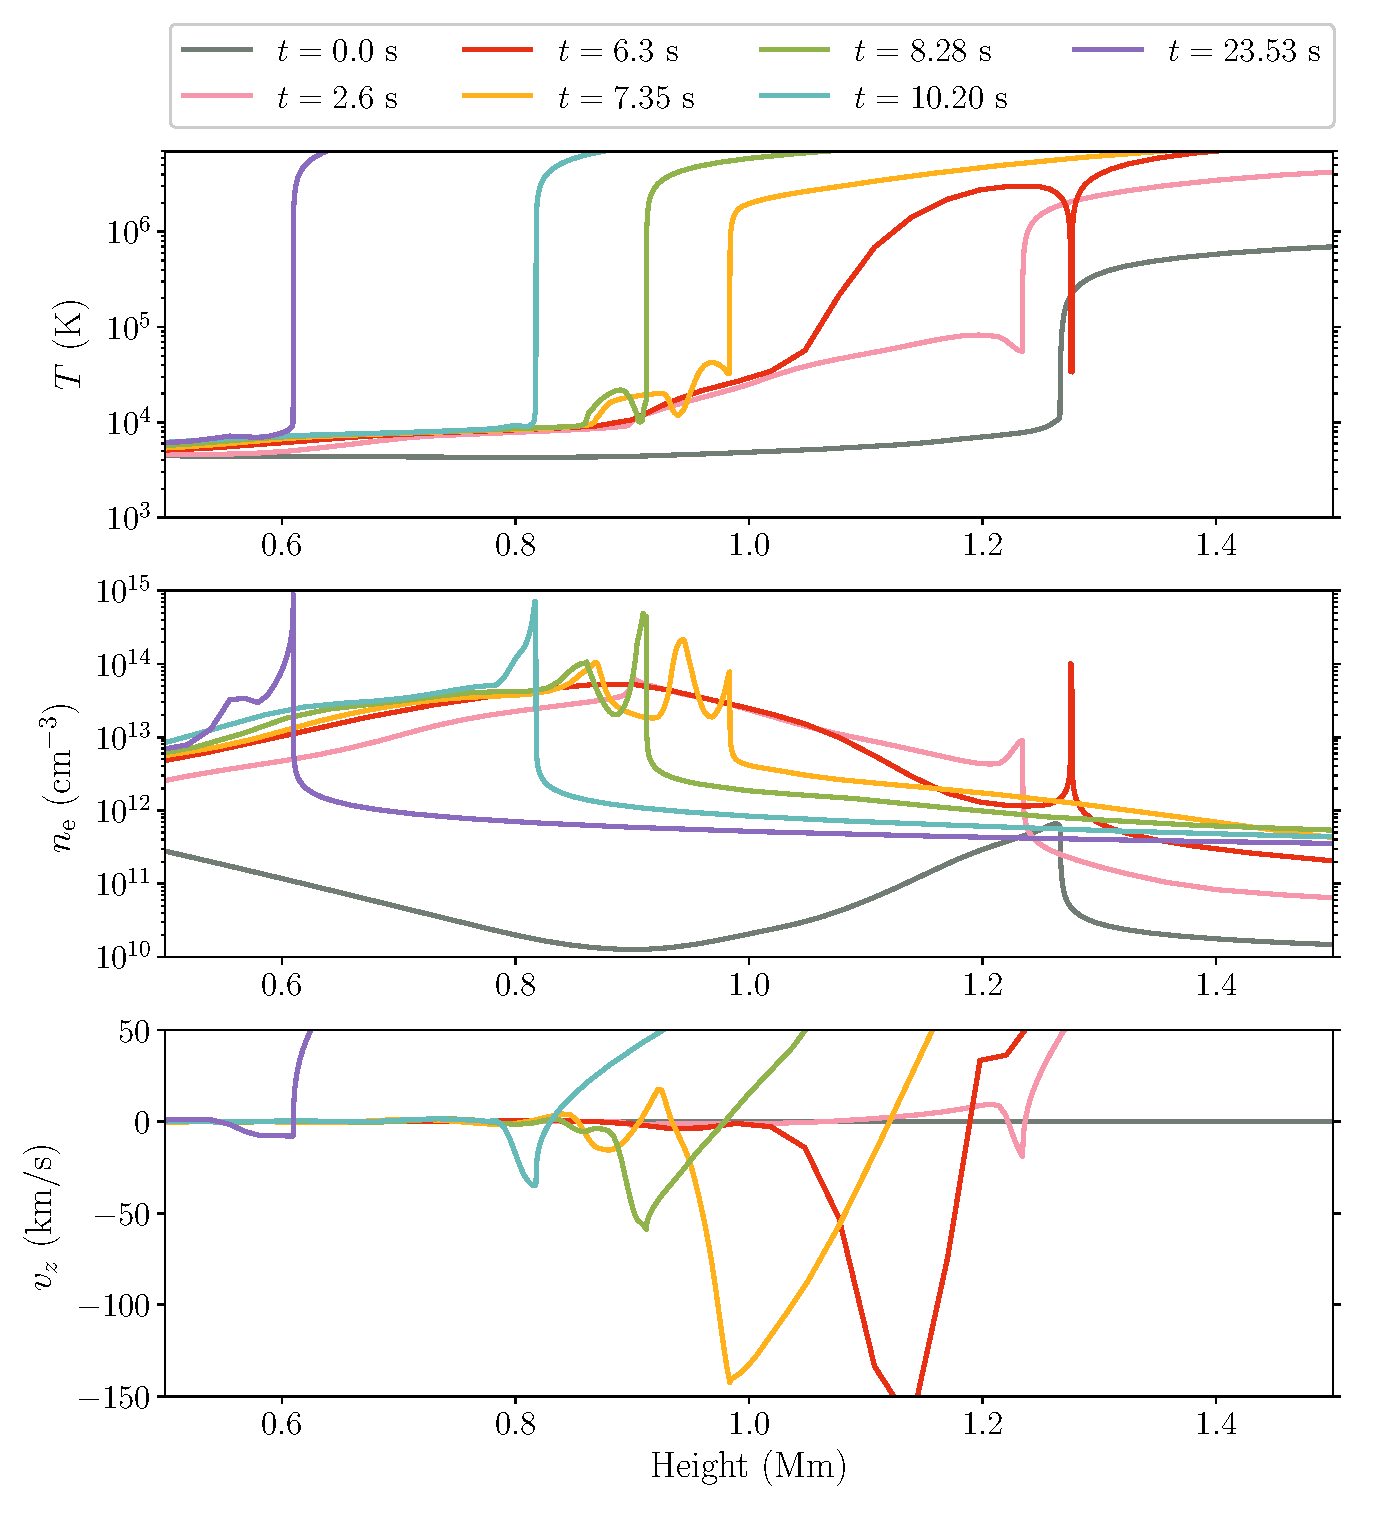
\includegraphics[width=0.8\textwidth]{figs/5F11_atmos_rev}
	\caption{5F11模型中的耀斑带上大气电子密度$n_e$、温度$T$和一维速度$v_z$随时间变化图。不同颜色的曲线代表模拟中的不同时刻。}
	\label{fig:3.1}
\end{figure}
我们在这一部分讨论RADYN代码得到的耀斑大气演化模型。图~\ref{fig:3.1}展示了电子密度$n_e$、温度$T$和一维速度$v_z$在模拟中的不同时刻在不同高度上的分布。可以看到整个大气结构随着非热电子束的不断加热发生了剧烈的变化,包含温度的上升、高色球的加热与剧烈的色球蒸发与凝聚过程。

在$t=2.6$ s时,高色球已经被剧烈加热至$3\times 10^4$ K。此时大气中的中性氢已经基本被完全电离,大气中的电子密度相比于初始大气已经上升了1-3个量级。在低日冕中约为1.25 Mm处,一个速度约为200 $\mathrm{km\  s^{-1}}$的色球蒸发过程已经出现。同时还伴随着过渡区和色球区域一个大约为20 $\mathrm{km\  s^{-1}}$的物质下流。由于色球顶部的加热,过渡区已经向下移动了大约25 km。

在$t=6.3$ s时,物质下流的体速度(\textit{bulk velocity})已经达到了约150 $\mathrm{km\  s^{-1}}$,且整个下流物质有大约100 km高。物质的向下流动拉伸的过渡区的高度,使其温度梯度减小。同时可以看到在日冕中有一团温度较低、电子密度较大的物质在向上传播。

在$t=7.35$ s时,下流物质逐渐到达较低的色球。由于色球密度远远高于过渡区密度,粒子的碰撞等一系列过程逐渐使得下流的体速度开始逐渐减小。之前被拉伸的过渡区位置又重新被压缩。同时这些相互作用也在过渡区下形成了一些电子密度较大$\sim 10^{14}\ \mathrm{cm}^{-3}$,但温度较低$\sim 1-2\times 10^{4}$ K的“团块”。这些团块在之后的时间内(如$t=8.28$ s)又逐渐随着过渡区的下移(物质的不断被加热)而并合在一起。

在$t=10$ s后,物质下流速度从40 $\mathrm{km\  s^{-1}}$继续减小,过渡区继续降低并压缩色球。相比于之前比较复杂的大气结构,整个大气变得趋于平静。在过渡区下方,形成了一个电子密度的高峰,达到了$5\times10^{14}-10^{15}\ \mathrm{cm^{-3}}$,接近\textcites{Rubio2017}中通过人工提高大气中的电子密度来实现Mg \textsc{ii}线的非线心反转的电子密度。

\begin{figure}
	\centering
	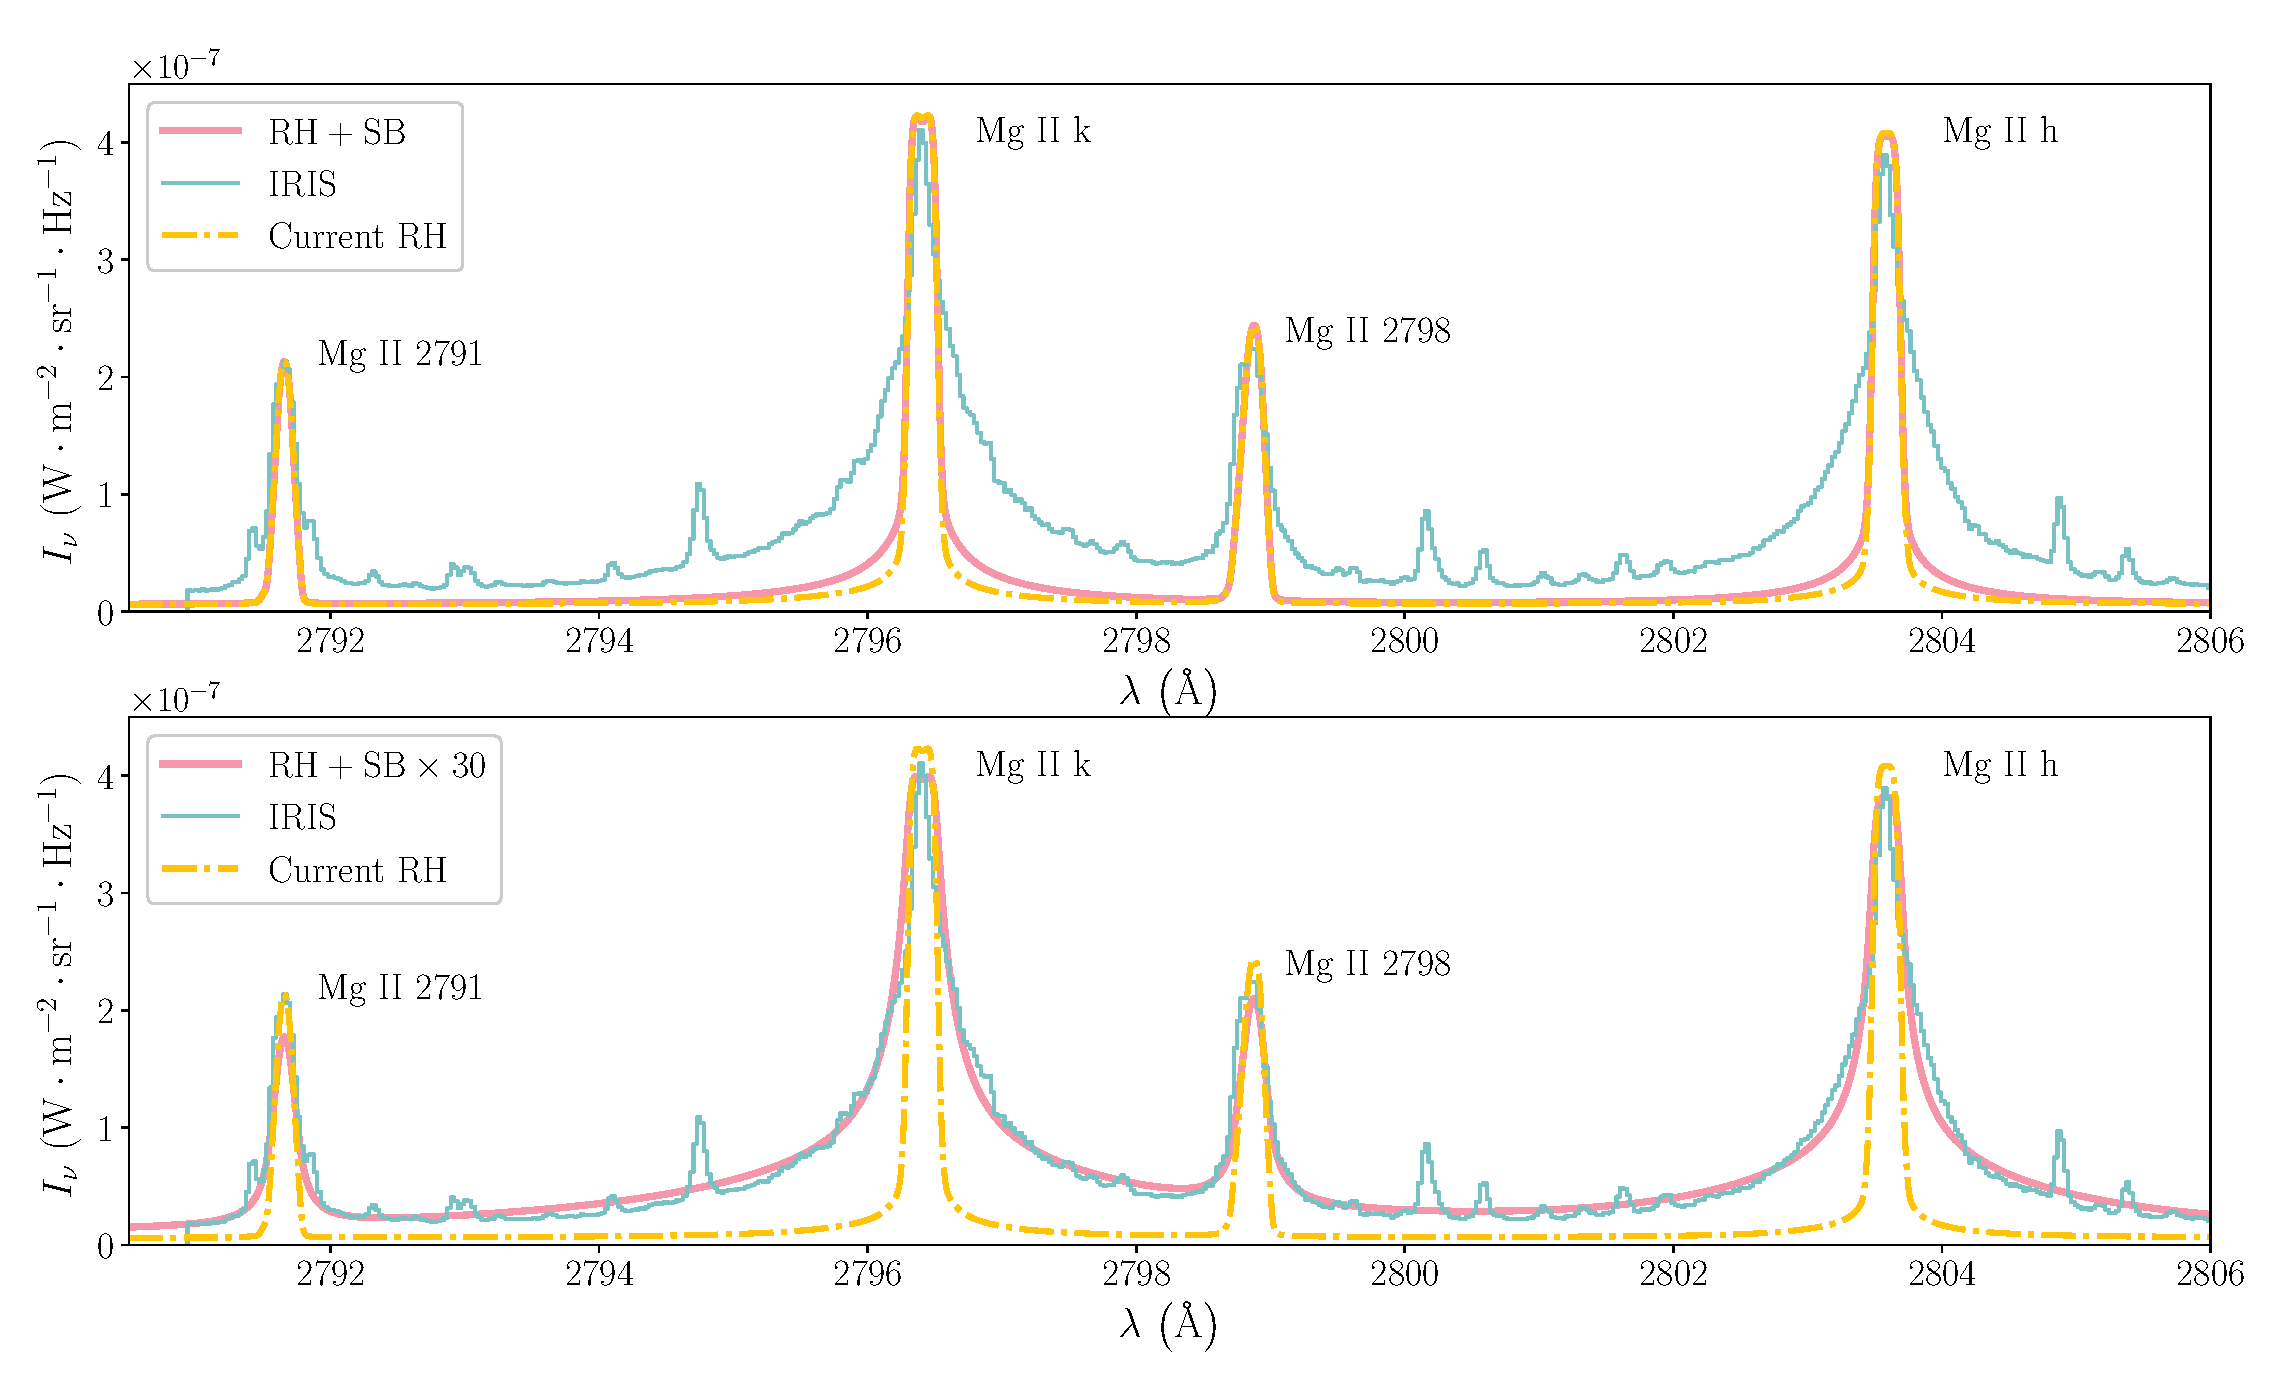
\includegraphics[width=\textwidth]{figs/MgII_SB}
	\caption{模拟中$t=23.53$ s时的Mg \textsc{ii}谱线轮廓与IRIS卫星观测的比较。黄色谱线轮廓代表未修改的RH代码得到的结果,蓝色谱线轮廓代表IRIS观测,上图中的粉色谱线代表RH+SB得到的结果,下图中的粉色谱线代表RH+SB$\times$30得到的谱线轮廓。经过辐射定标(\textit{radiometric calibration})后的IRIS观测数据被乘上了一个36的因子来获得与RH合成光谱相近的辐射强度。这个填充因子(\textit{filling factor})可能来自于IRIS观测的分辨率限制。}\label{fig:3.2}
\end{figure}

\section{谱线演化:Mg \textsc{ii}}\label{sec:3.4}
在这一部分中我们将讨论Mg \textsc{ii}谱线轮廓在模拟中的演化以及和IRIS观测到的耀斑带上的谱线轮廓的对比。对于Mg \textsc{ii} h和k线而言,在大的耀斑带上能够观测到两种特征的谱线轮廓,一种是带有很强的红翼不对称性,另一种是比较对称,无线心反转且线翼剧烈增宽的谱线\parencites{Panos2018}。我们这里主要尝试再现第二种谱线,对前者我们仅对其可能出现的原因进行简单的讨论。在具体模拟中,我们使用了一个10能级的Mg \textsc{ii}原子模型,包含Mg \textsc{ii}基态(Mg \textsc{i}连续态)和连续态(Mg \textsc{iii}基态)来计算辐射转移。

在图~\ref{fig:3.2}中,我们展示了$t=23.53$ s时合成(\textit{synthetic})的Mg \textsc{ii}谱线轮廓和IRIS观测的比较。可以看到RH代码比较好地再现了Mg \textsc{ii}线非线心反转的谱线特征,且使用STARK-B数据库后的RH代码(以下记为RH+SB)给出了比原有RH代码更加宽且增强的线翼辐射,但相比于IRIS观测(蓝线)中剧烈的线翼增强还是有比较大的差距。针对这一点,我们进行了一个大胆的尝试,我们直接在STARK-B数据库中所有Mg \textsc{ii}谱线的$\Gamma_{stark}$上乘了一个30的因子(以下记作RH+SB$\times$30)。在这样的处理之后,我们能够获得了和观测拟合的非常好的谱线轮廓,预示着Mg \textsc{ii}线间的连续谱辐射增强可能来自于这些谱线剧烈增强的线翼辐射。

\begin{figure}
	\centering
	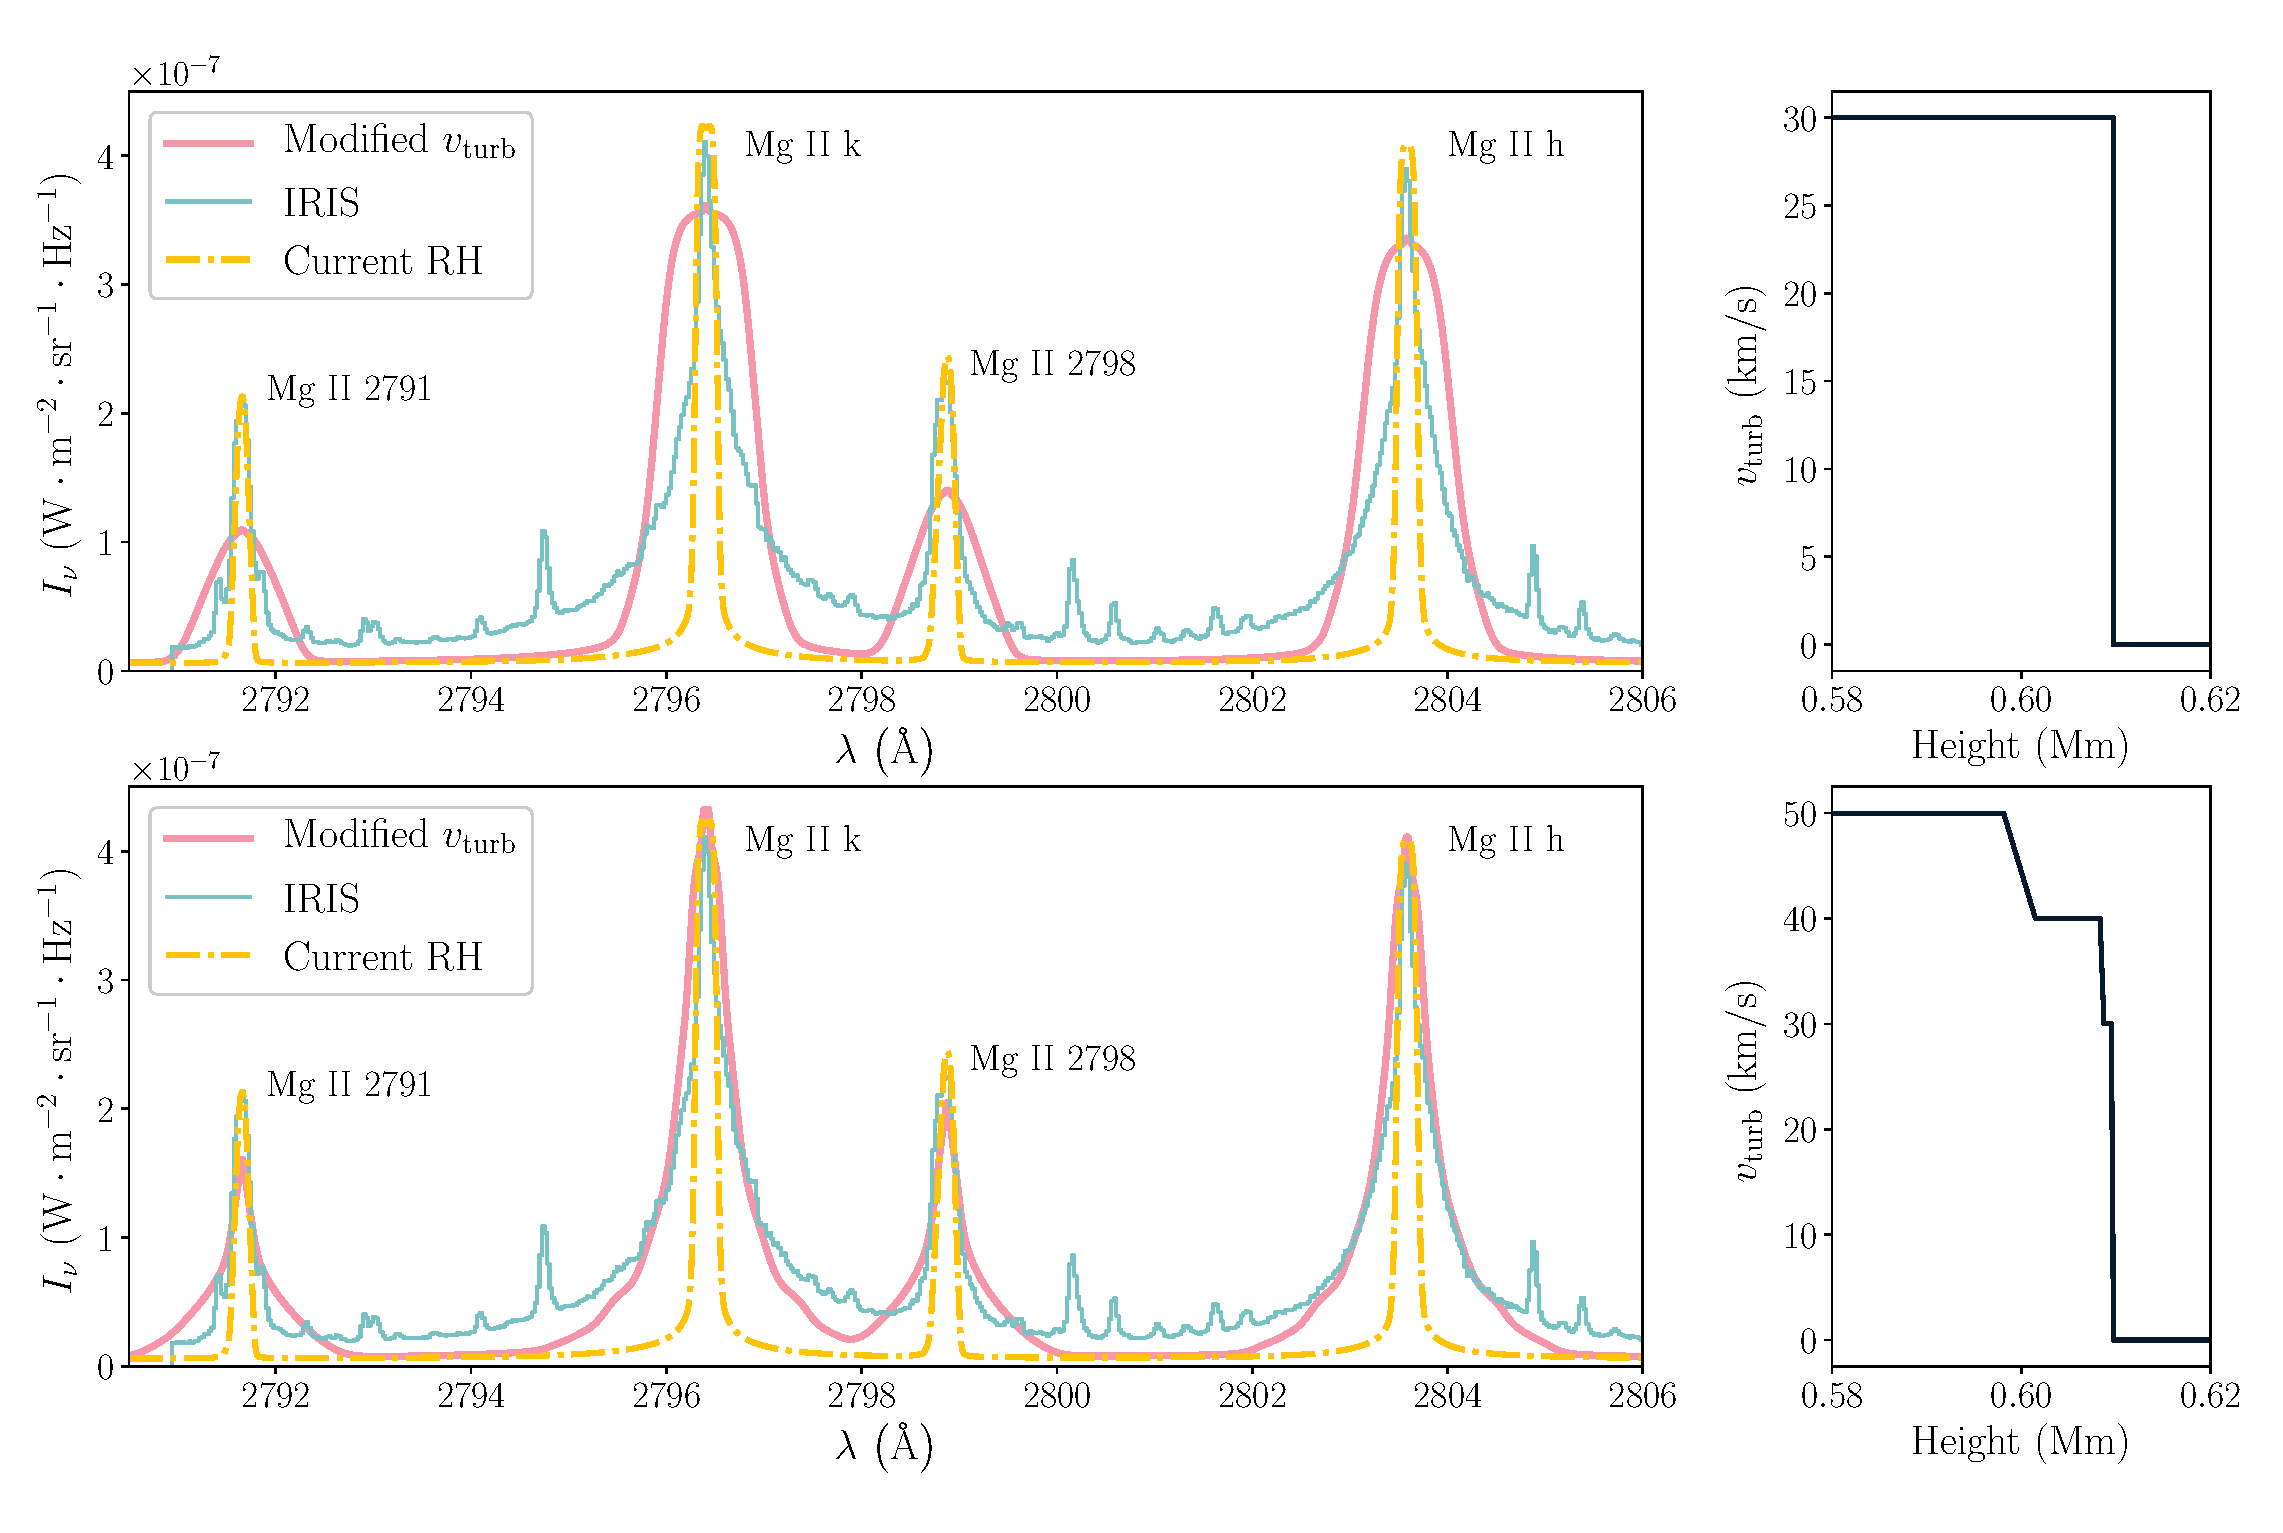
\includegraphics[width=\textwidth]{figs/MgII_vturb}
	\caption{通过调节大气中的微湍动速度分布来实现Mg \textsc{ii}谱线的致宽。上图粉色轮廓来自恒定的$30\ \mathrm{km \  s^{-1}}$的湍动速度的耀斑大气,下图粉色轮廓来自湍动速度从线心形成高度逐渐增加到$50\ \mathrm{km \  s^{-1}}$的耀斑大气。}\label{fig:3.3}
\end{figure}

为了排除诸如微湍动速度等因素对谱线致宽的影响,我们尝试人工调节RADYN输出大气中的湍动速度在不同高度的分布来观察Mg \textsc{ii}谱线的轮廓变化。我们在同图~\ref{fig:3.2}中相同时刻的大气中插入了两种湍动速度的分布,一种是恒定的$30\ \mathrm{km \  s^{-1}}$的湍动速度(图~\ref{fig:3.3}上半图),另一种是从线心形成高度逐渐增加到$50\ \mathrm{km \  s^{-1}}$(图~\ref{fig:3.3}下半图)。从图~\ref{fig:3.3}中可以看出对于前者来说,由于在RH代码中湍动速度的分布是Gaussian形的,因此过大的湍动速度直接导致了整个谱线的形状都被Gaussian形的谱线所主导,这样的谱线轮廓在线心处太宽,且在线翼处增强不大,因此不能较好的再现谱线的致宽。而对于后者而言,虽然我们能够通过从线心开始逐渐增加湍动速度来达到使Mg \textsc{ii} h和k线轮廓与观测符合的比较好的结果,但是由于Mg \textsc{ii}三重线和Mg \textsc{ii} h,k两线在此时的形成高度相近,导致了合成的Mg \textsc{ii}三重线相比于观测到的谱线轮廓更加宽了。因此我们认为提高微湍动速度并不是解释谱线剧烈致宽的主要机制。

\begin{figure}
	\centering
	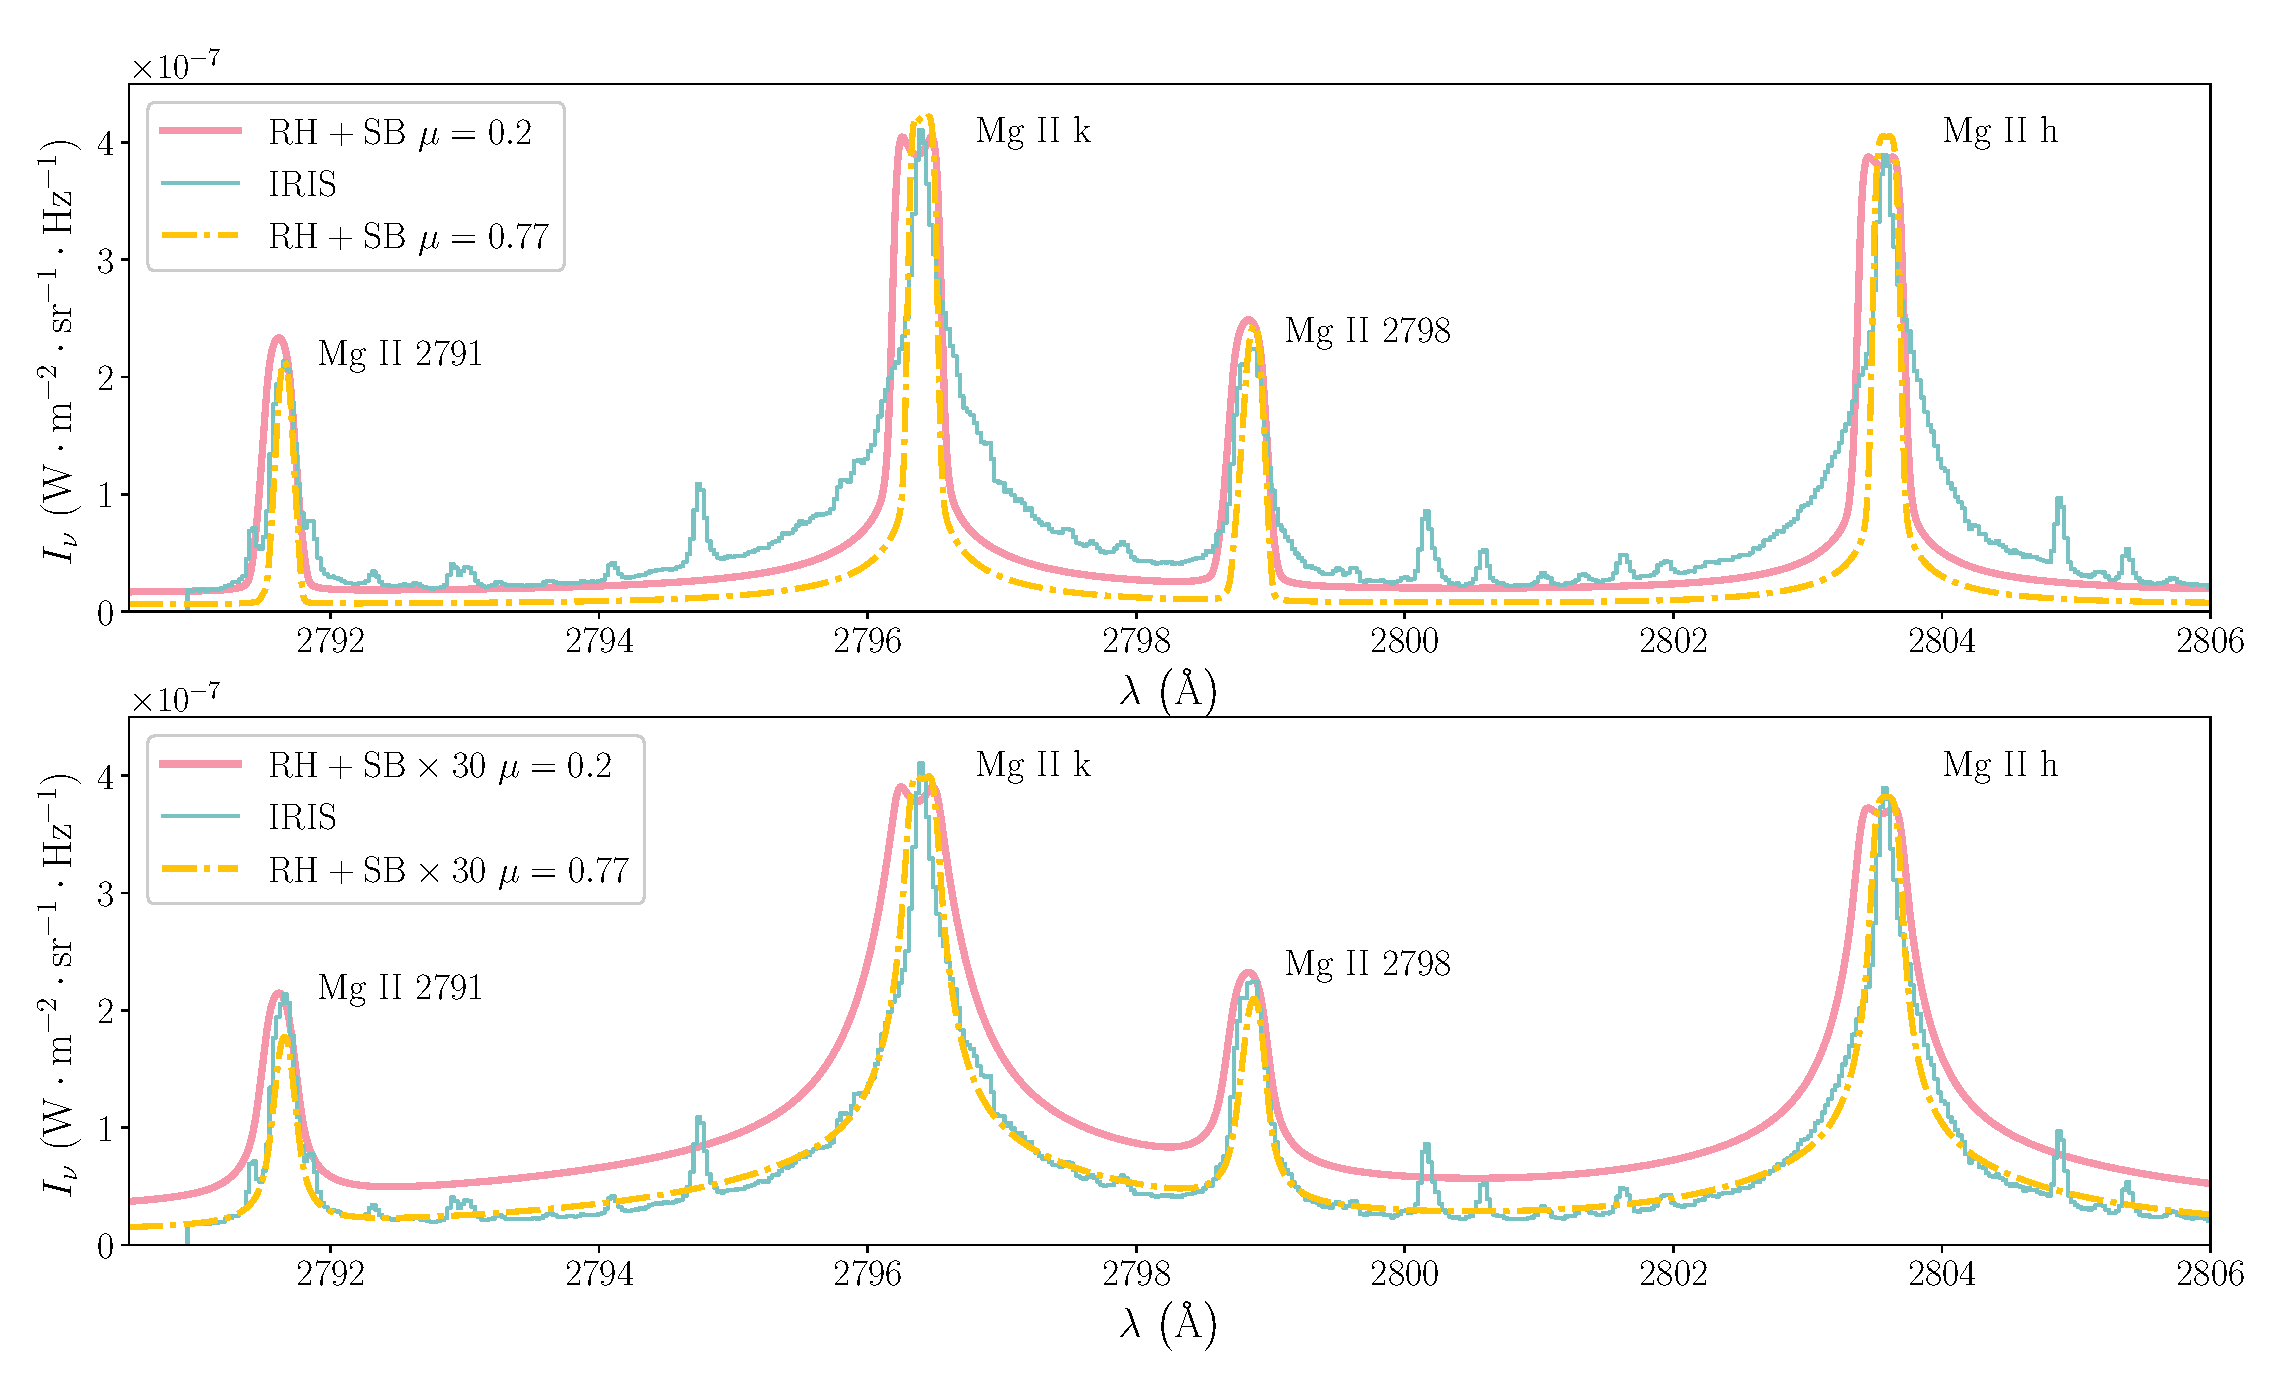
\includegraphics[width=\textwidth]{figs/MgII_mu02}
	\caption{模拟中$t=23.53$ s时在不同方向角$mu$下计算的合成Mg \textsc{ii}谱线轮廓与IRIS卫星观测的比较。上半图为RH+SB中$\mu=0.2$(粉色实线)和$\mu = 0.77$(黄色点划线)下的合成谱线轮廓。下半图为为RH+SB$\times$30中$\mu=0.2$(粉色实线)和$\mu = 0.77$(黄色点划线)下的合成谱线轮廓。}
	\label{fig:3.3.5}
\end{figure}

最后,我们还讨论了视线方向角$\mu$对Mg \textsc{ii}谱线轮廓的影响。在图~\ref{fig:3.3.5}中我们比较了在RH+SB和RH+SB$\times$30中$\mu=0.2$和$\mu=0.77$。$\mu$越小,说明视线方向和平面平行层大气的法线方向夹角越大(对太阳观测而言越靠近临边)。$\mu = 0.2$的谱线轮廓与$\mu = 0.77$的谱线轮廓相比,线翼辐射更强,红移越小(投影速度小),且谱线线心反转越明显。这一现象的简单解释可以参见\ref{sec:3.7}节。

\begin{figure}[htbp]
	\begin{minipage}[t]{0.48\linewidth}
	\centering
	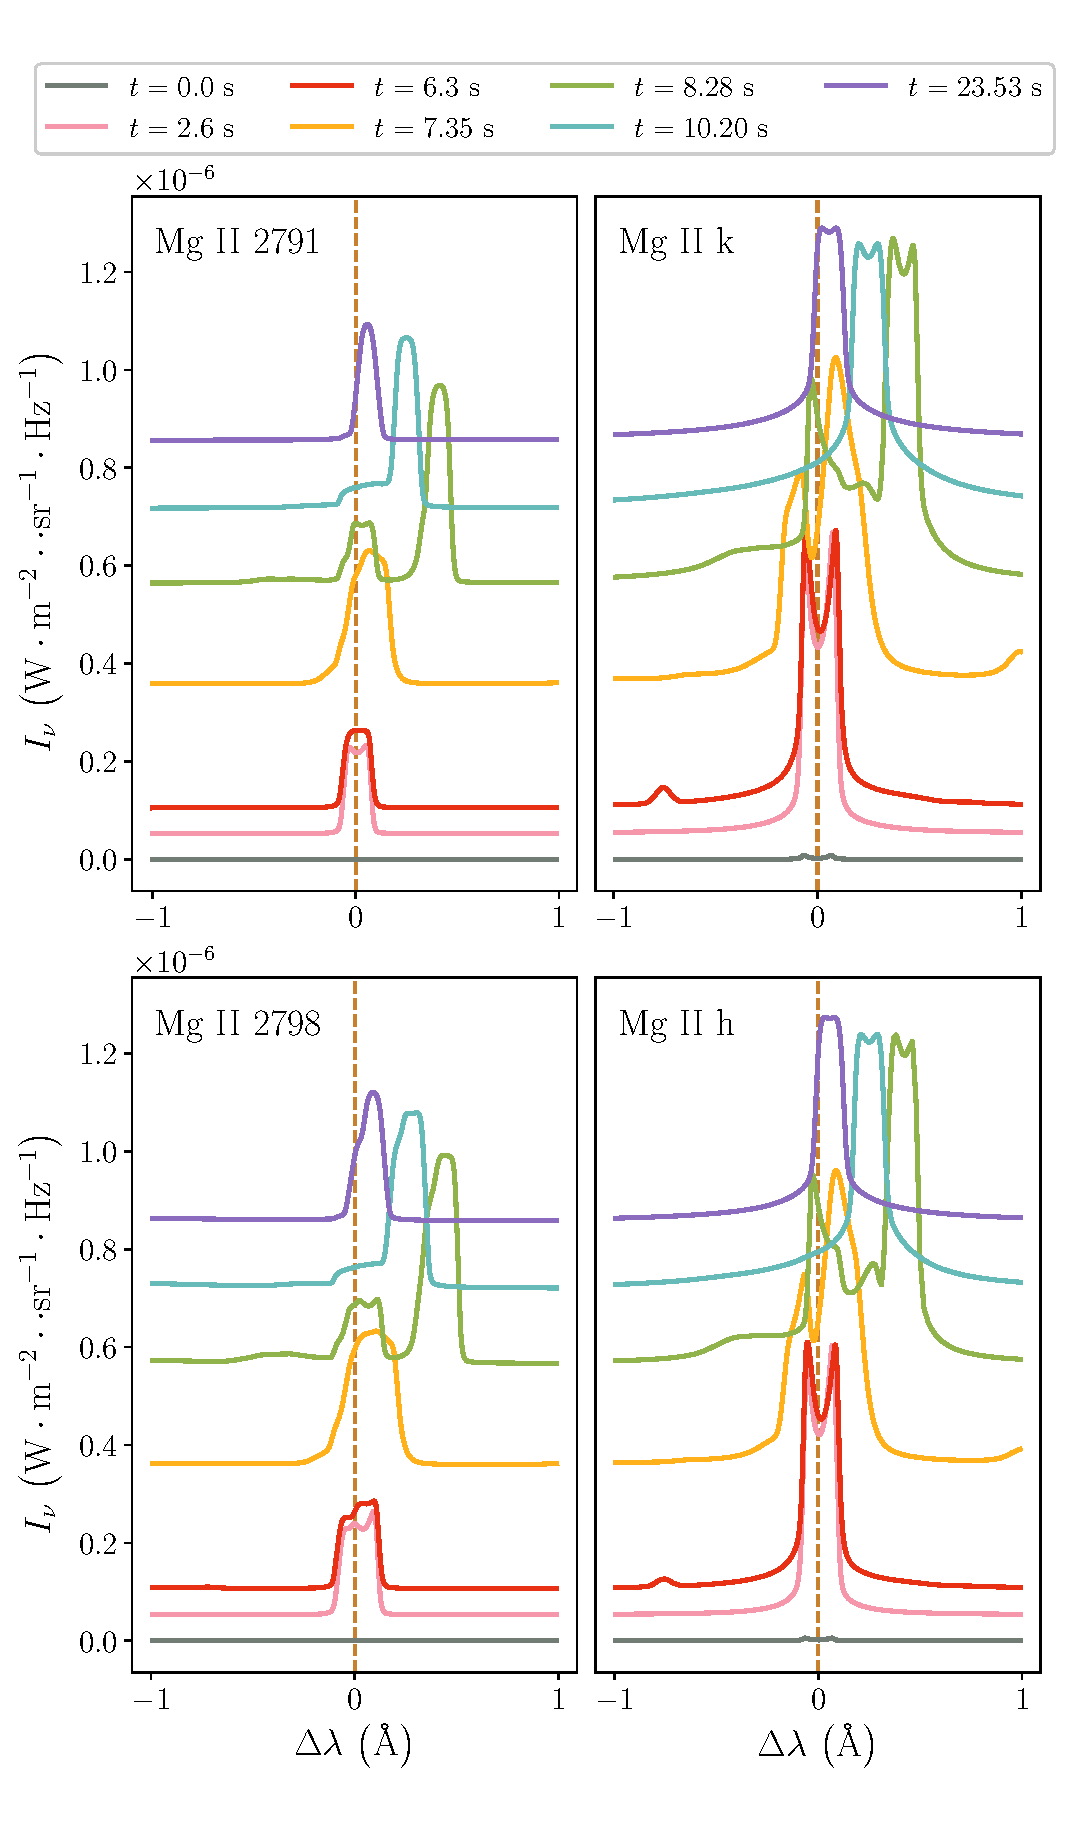
\includegraphics[width=0.95\linewidth]{figs/5F11_spectra_1_mg}
	\end{minipage}%
	\hfill
	\begin{minipage}[t]{0.48\linewidth}
	\centering
	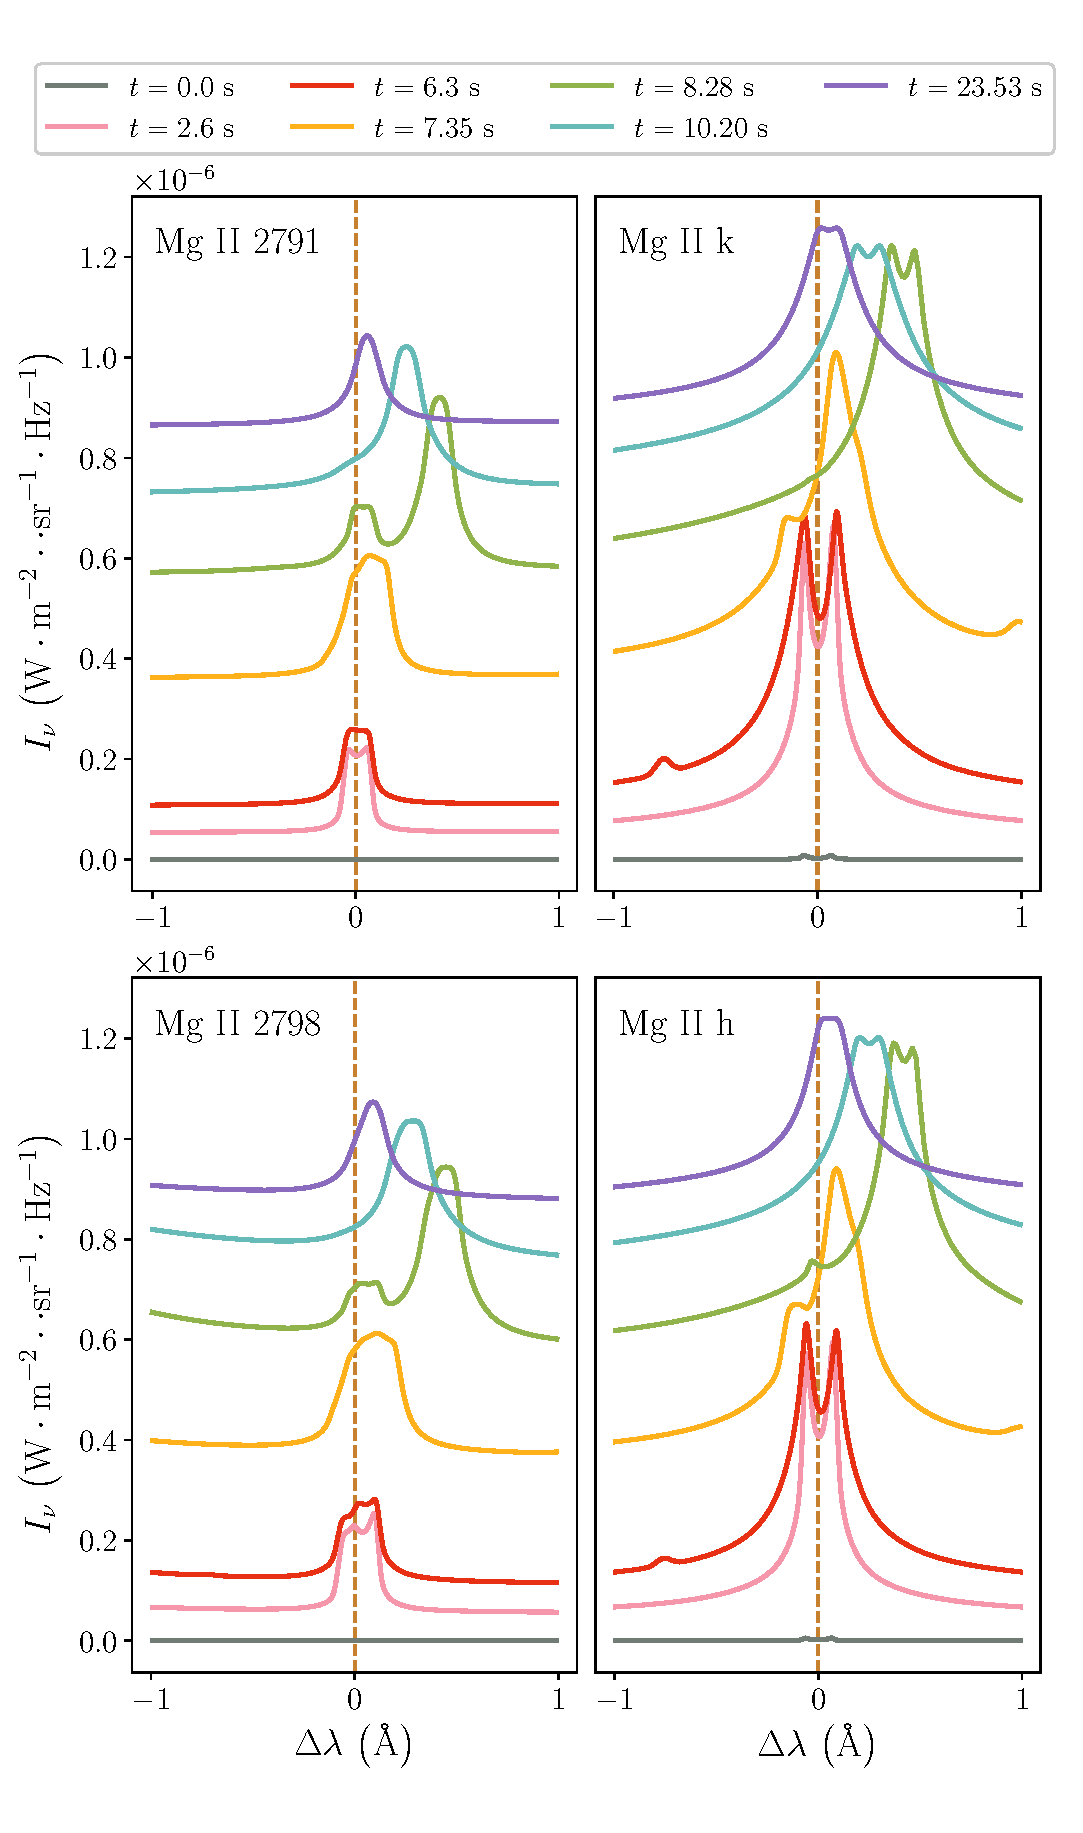
\includegraphics[width=0.95\linewidth]{figs/5F11_spectra_2_mg}
	\end{minipage}
	\caption{RH+SB(左)和RH+SB$\times30$(右)下的Mg \textsc{ii}合成谱线轮廓演化。为了能够清楚地显示不同时刻的轮廓,不同时刻的谱线轮廓被人为向上移动了一段距离。}
	\label{fig:3.4}
\end{figure}


基于以上的研究,我们分别在RH+SB和RH+SB$\times30$下计算了Mg \textsc{ii}各条谱线在整个演化过程中的轮廓(图~\ref{fig:3.4})。在$t=2.6$ s和$t=6.3$ s,由于低层大气已经被非热电子束剧烈加热,Mg \textsc{ii}各条线的辐射强度均有剧烈增强。两套计算方法中此时的谱线轮廓仍存在线心反转,同样来自于在线心形成高度源函数和Planck函数的脱耦\parencites{Rubio2016}。

在$t=7.35$ s时,Mg \textsc{ii} h,k和三重线都明显增宽,这主要来自于此时速度上流和下流中都对Mg \textsc{ii}谱线形成有所贡献导致的两个不同Doppler频移的分量的叠加。在RH+SB$\times30$中有更多的光子因为Stark致宽而被散射到线翼上,因此相比于RH+SB的结果,其线心反转反而不再明显。

在$t=8.28$ s时,所有的Mg \textsc{ii}线都出现了一个静止分量和一个红移分量,这个红移分量来自于速度下流部分物质对Mg \textsc{ii}线辐射的贡献。这些谱线在观测中都不太常见,但我们猜测耀斑带前缘的红翼不对称的Mg \textsc{ii}谱线可能来自于这些红移分量的叠加效应,之前\textcites{Rubio2016}的多环(\textit{multi-thread})的模拟也指出了这一点。

在$t=10$ s后,Mg \textsc{ii}线的红移随着速度下流的逐渐减小而减小。此时Mg \textsc{ii}的线心形成高度正好处于过渡区下的高电子密度区域(详细分析见\ref{sec:3.7}节),较高的电子密度维持了一个近似于LTE的环境,使得线心源函数与Planck函数的脱耦并不明显,线心反转消失。由于Stark致宽效应主要发生在线翼区域,因此其仅仅产生了更加增强的线翼辐射。

\section{谱线演化:C \textsc{ii}}

\begin{figure}
	\centering
	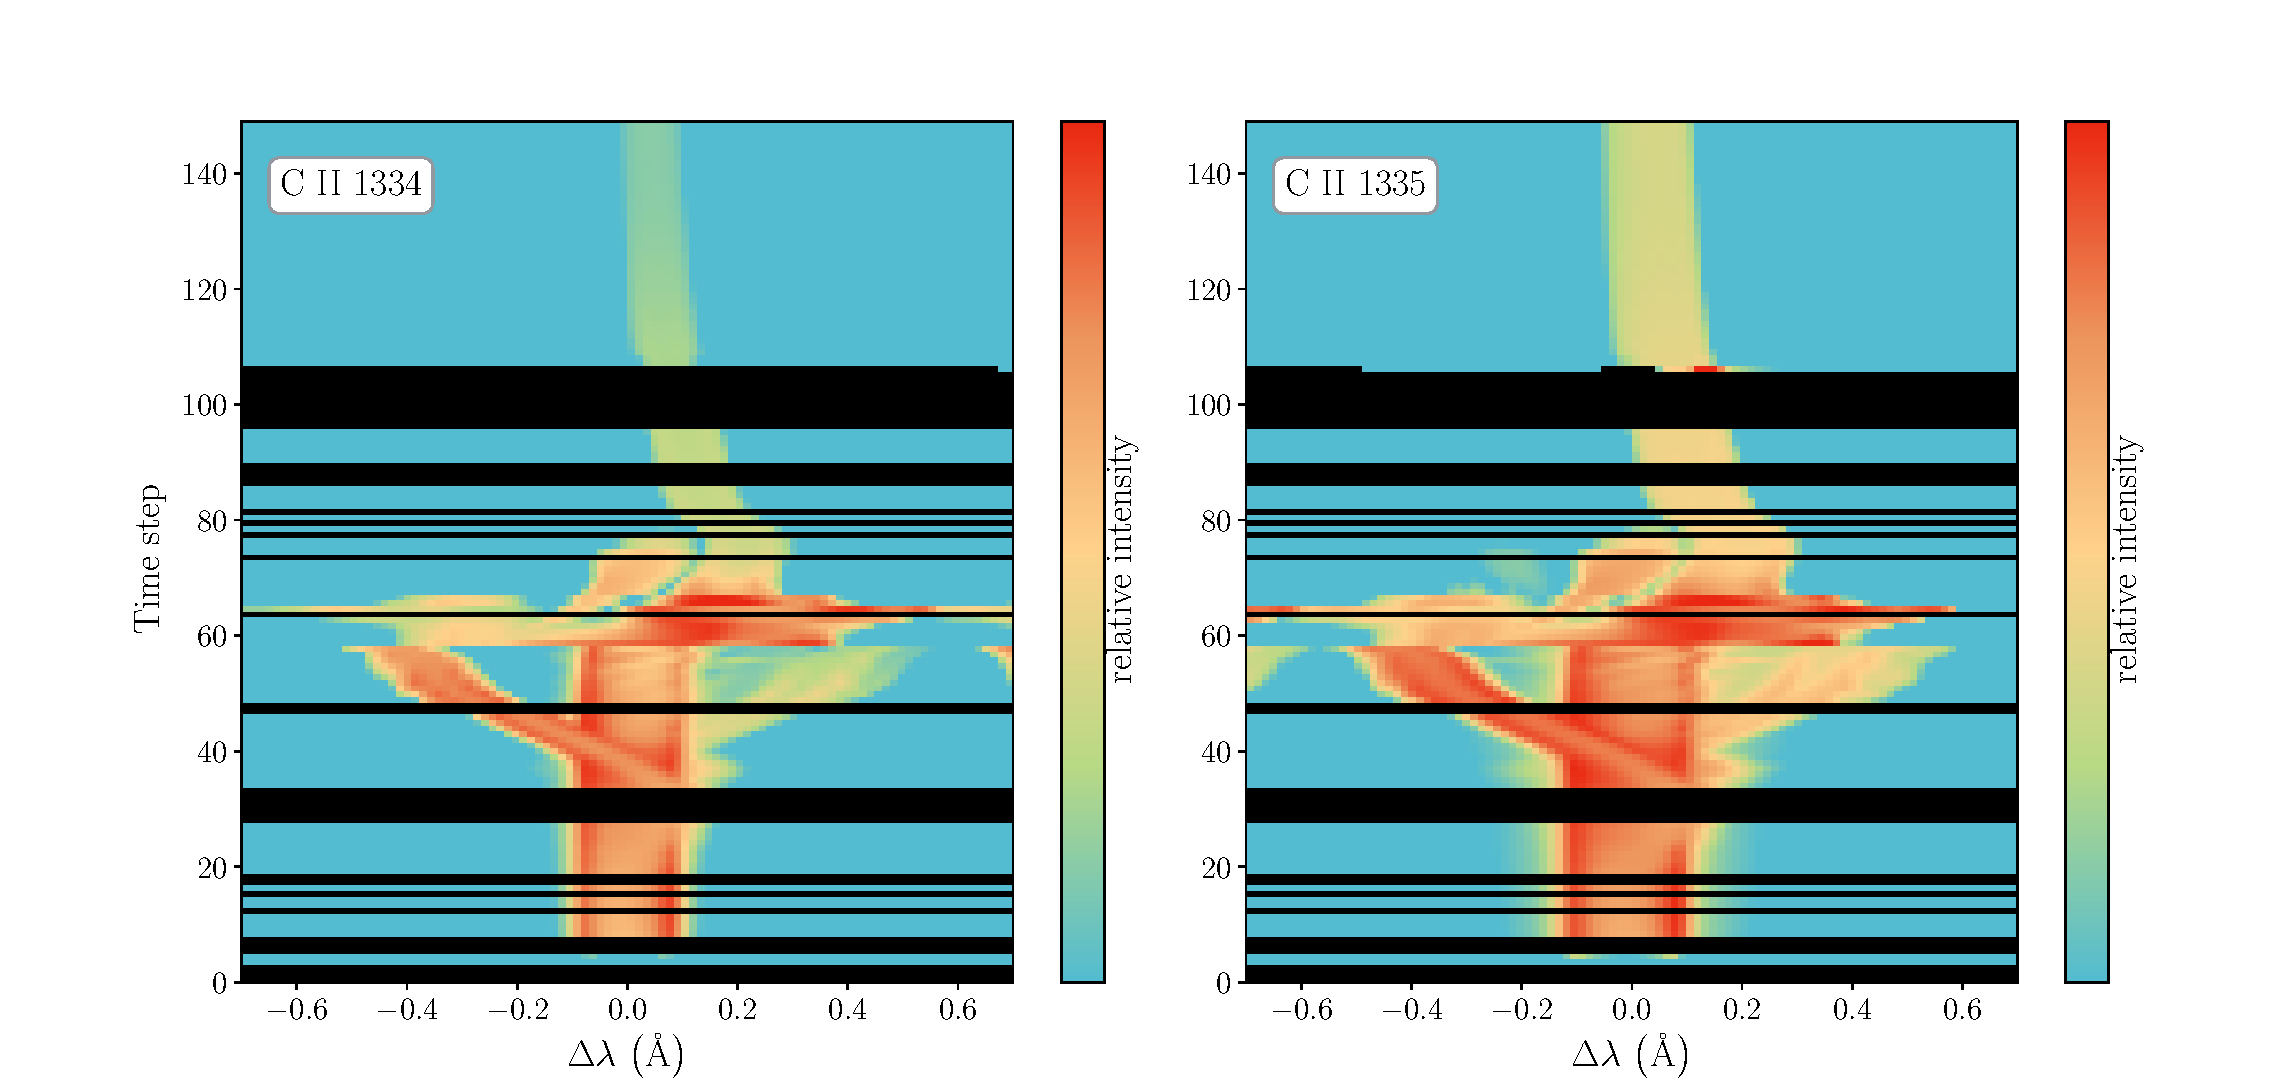
\includegraphics[width=\textwidth]{figs/5F11_spectra_imshow_C}
	\caption{C \textsc{ii}双重线强度随时间演化图,横坐标为波长,纵坐标为不同时刻,颜色代表该波长和时刻下的辐射强度。图中黑色部分为为由于数值原因无法收敛或者出现运算崩溃的时刻。}
	\label{fig:3.5}
\end{figure}

在这一部分我们将讨论基于同样的RADYN耀斑大气演化所计算的C \textsc{ii}双重线的谱线轮廓演化。此处我们使用了RH代码自带的一个9能级的C \textsc{i}和C \textsc{ii}原子模型,包含C \textsc{i}的三个能级和6个C \textsc{ii}的能级。图~\ref{fig:3.5}展示了这两条线在所有能够正确计算的时刻其谱线内的辐射强度随着时间的演化。图中的黑色区域为由于数值原因无法收敛或者出现运算崩溃的时刻。同时我们还挑选了一些计算收敛且有代表性的谱线轮廓展示在图~\ref{fig:3.6}中。这些时刻的问题可能来自于在高温度时计算碰撞电离时的LU分解出现奇异性。
\begin{figure}
	\centering
	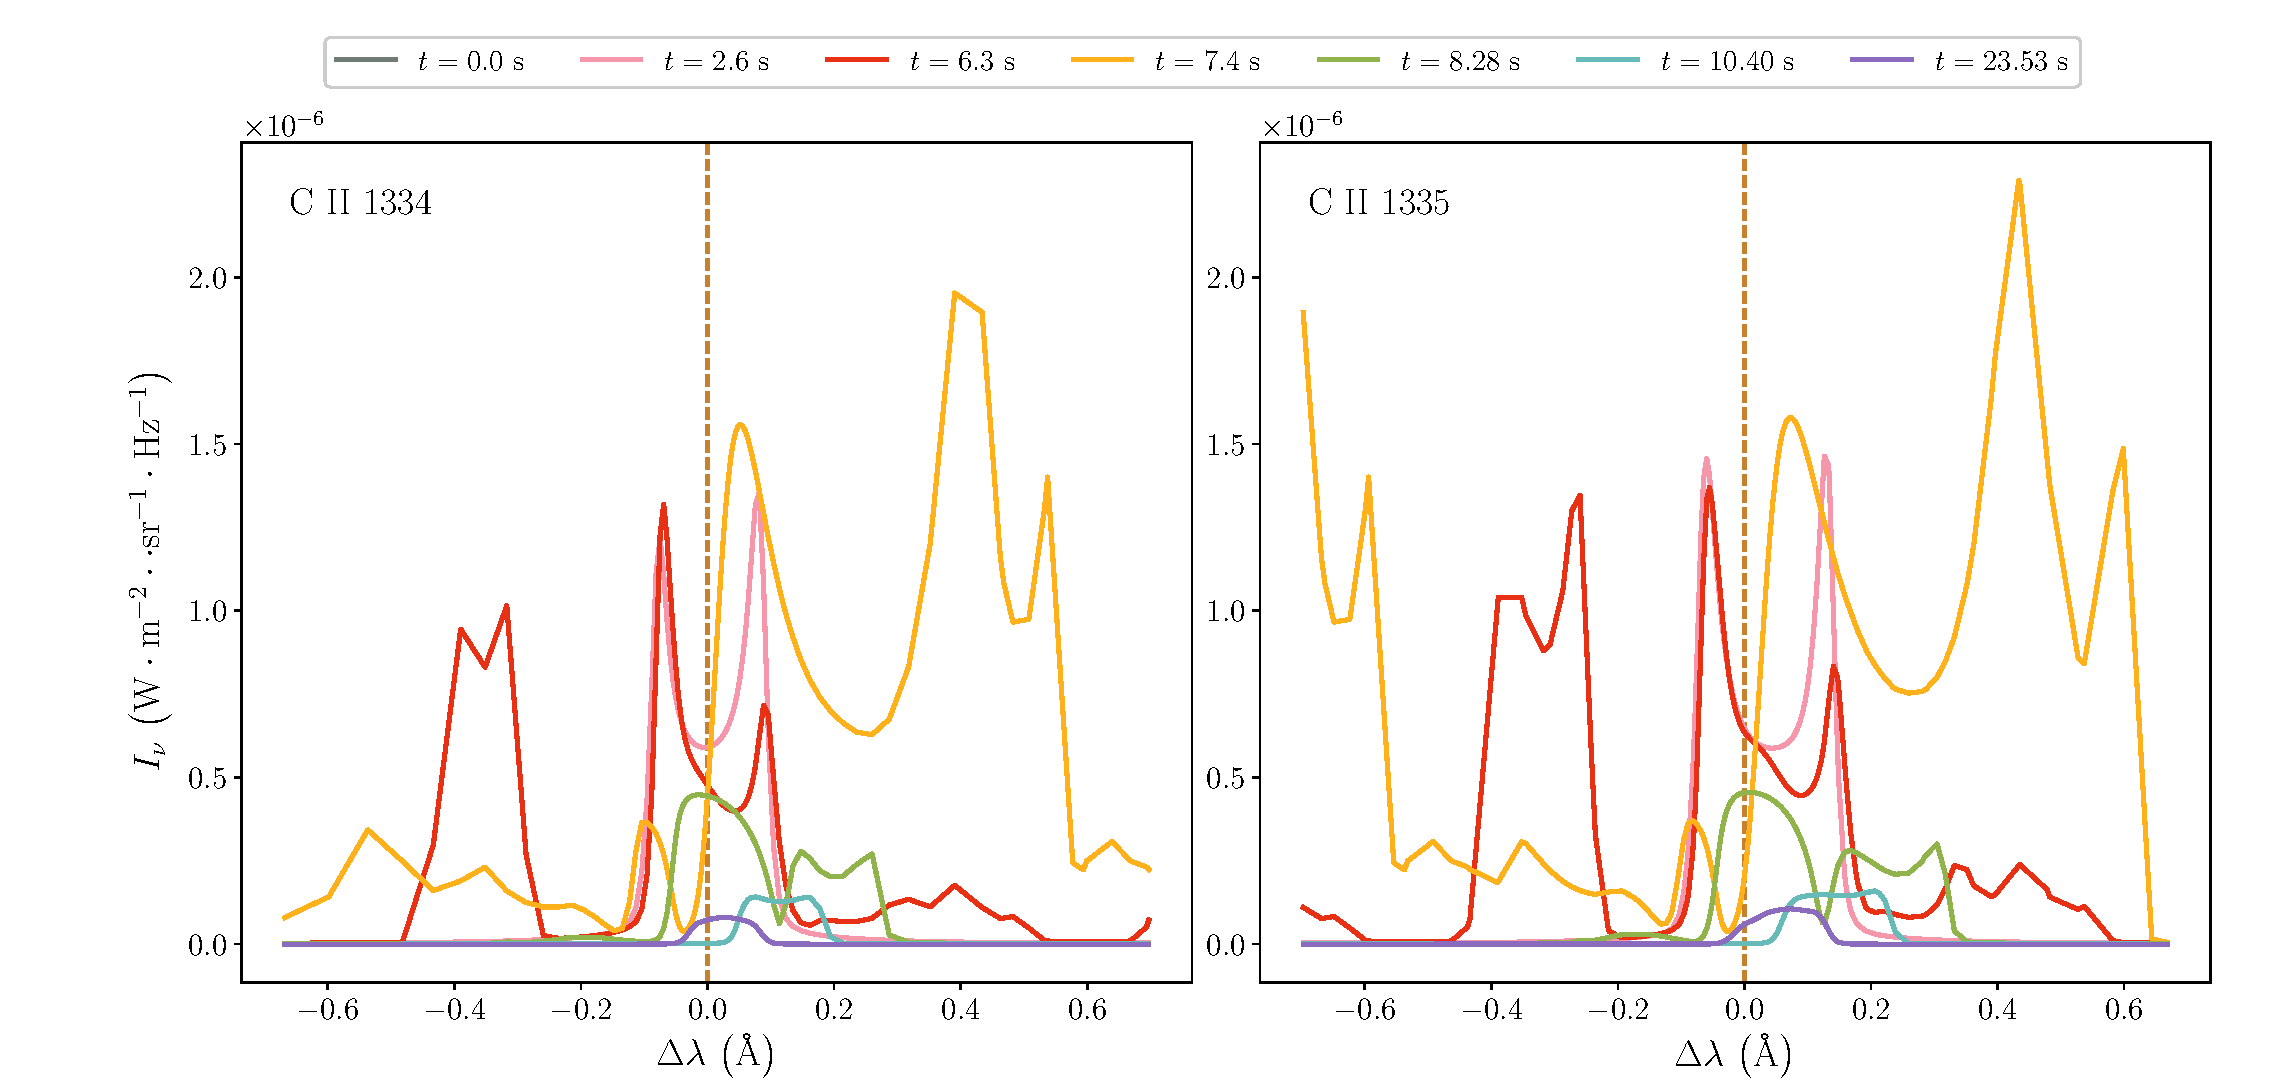
\includegraphics[width=\textwidth]{figs/5F11_spectra_line_C}
	\caption{和图~\ref{fig:3.1}中时刻相近大气中计算得到的C \textsc{ii}双重线谱线轮廓。}
	\label{fig:3.6}
\end{figure}


总体上来说,我们可以大致描述整个C \textsc{ii}线的轮廓随时间演化的大致趋势。在前2 s左右,整个谱线还处在线心反转的大致形状中(图~\ref{fig:3.6}中$t=2.6$ s的粉色轮廓)。在$2-4$ s间,原来线心反转中的蓝翼峰不断增强,红翼峰不断减弱,形成了一个有明显蓝翼增强的谱线。之后在$t=6 s$左右随着色球凝聚的出现以及一个向上运动冷且密度较大的物质流的出现,C \textsc{ii}谱线出现了一个蓝移分量和一个红移分量(如$t=6.3$ s时的红色轮廓)。在$t=7$ s左右,物质下流的速度达到最大,C \textsc{ii}谱线出现了剧烈的红翼不对称性(图~\ref{fig:3.6}中黄色轮廓)。在$t=8$ s后谱线强度逐渐减弱,和Mg \textsc{ii}线类似出现了一个静止分量和一个红移分量(推测来自于两条线形成高度随着色球压缩而不断靠近)。之后的谱线轮廓演化也和Mg \textsc{ii}线类似,在$t=10$ s后静止分量基本消失,谱线红移逐渐减小,发射强度也随之降低(图~\ref{fig:3.6}中)。由于存在着另一条谱线的重叠,C \textsc{ii} 1335 \mbox{\AA}线的轮廓和1334 \mbox{\AA}的轮廓略有不同,谱线内积分强度较大,但是没有本质上的区别。

由于之前在图~\ref{fig:3.2}中$t=23.53$ s的Mg \textsc{ii}谱线轮廓在RH+SB$\times30$中的计算与观测取得了比较好的结果,我们同样比较了同一时间的合成光谱中的C \textsc{ii}双重线轮廓与耀斑带上同一地点同一时间的C \textsc{ii}线观测轮廓(图~\ref{fig:3.7})。我们发现尽管合成光谱中Mg \textsc{ii}线的Doppler频移能够和具体观测得到比较好的拟合,但是合成的C \textsc{ii}线与实际观测到的C \textsc{ii}线红移不太相符。即我们没有办法在模拟中同时比较好地再现C \textsc{ii}线和Mg \textsc{ii}线轮廓。在利用C \textsc{i} 1354.288 \mbox{\AA}线对FUVS部分的谱线进行严格的波长定标之后,我们发现如图~\ref{fig:3.7}上半图中粉色轮廓所示,其线心位置和IRIS观测到的线心大约相距$\sim 0.062$ \mbox{\AA},折合约为$\sim 14\ \mathrm{km\  s^{-1}}$。在模拟当中红移和观测大致相符的谱线大约出现在$t=13.0$ s左右(图~\ref{fig:3.7}中黄色点划轮廓)。

由于STARK-B数据库中并没有这C \textsc{ii}这几条谱线的Stark致宽数据,但是从图~\ref{fig:3.7}上半图中可以明显看出谱线在远线翼致宽仍然远远不足。受之前的Mg \textsc{ii}线的调整启发,我们直接在RH代码中人工调整$\Gamma_{Stark}$。我们发现,如果要让$t=23.53$ s和$t=13.0$ s的红侧远线翼产生足够的辐射增强,需要在$t=23.53$ s的$\Gamma_{Stark}$乘上一个约为740的因子,或者在$t=13.0$ s的谱线的$\Gamma_{Stark}$上乘上一个290的因子。此外,我们的谱线尚不能很好的再现在蓝翼的一些辐射增强。

\begin{figure}
	\centering
	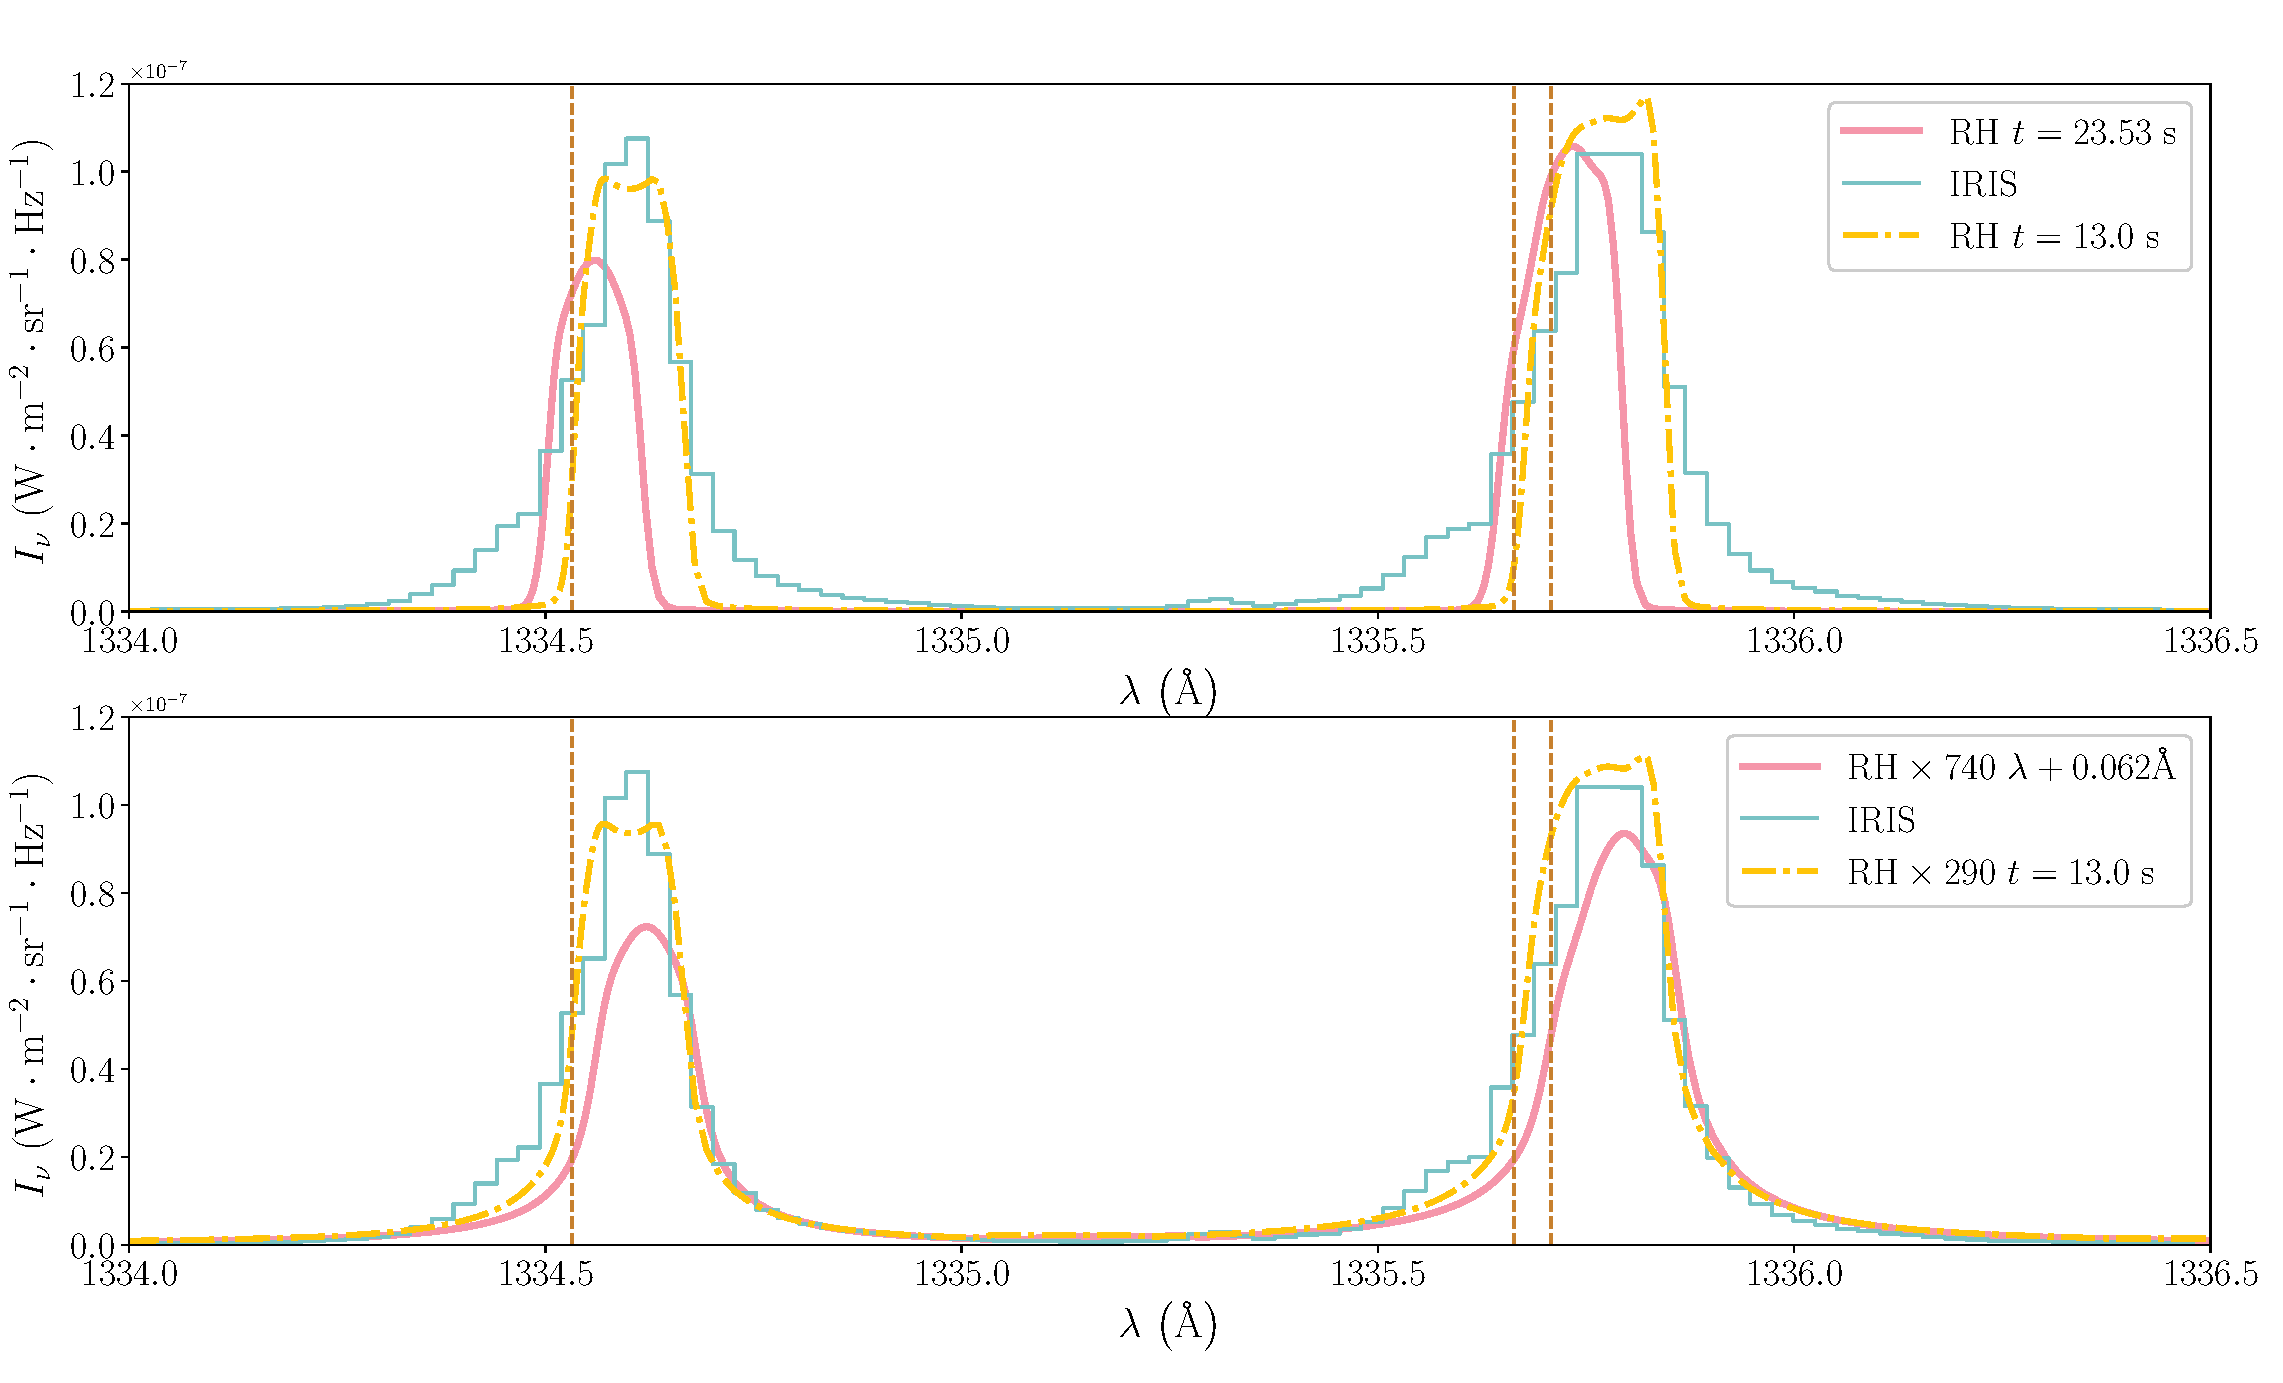
\includegraphics[width=\textwidth]{figs/5F11_IRIS_CII}
	\caption{合成的C \textsc{ii}双重线与IRIS观测的比较。上半图中展示了RH代码输出中$t=23.53$ s和$t=13.0$ s的谱线轮廓和IRIS观测的对比,下半图展示了通过人工增加Stark致宽和移动波长得到的$t=23.53$ s的谱线轮廓、仅增加Stark致宽得到的$t=13.0$ s的谱线轮廓和IRIS观测的对比。其中竖线代表了三条C \textsc{ii}线的真空静止波长。其中的IRIS观测经过辐射定标之后同样乘了一个10的因子使其强度与RH合成光谱可比。}
	\label{fig:3.7}
\end{figure}

\section{谱线演化:Si \textsc{iv}}
\begin{figure}
	\centering
	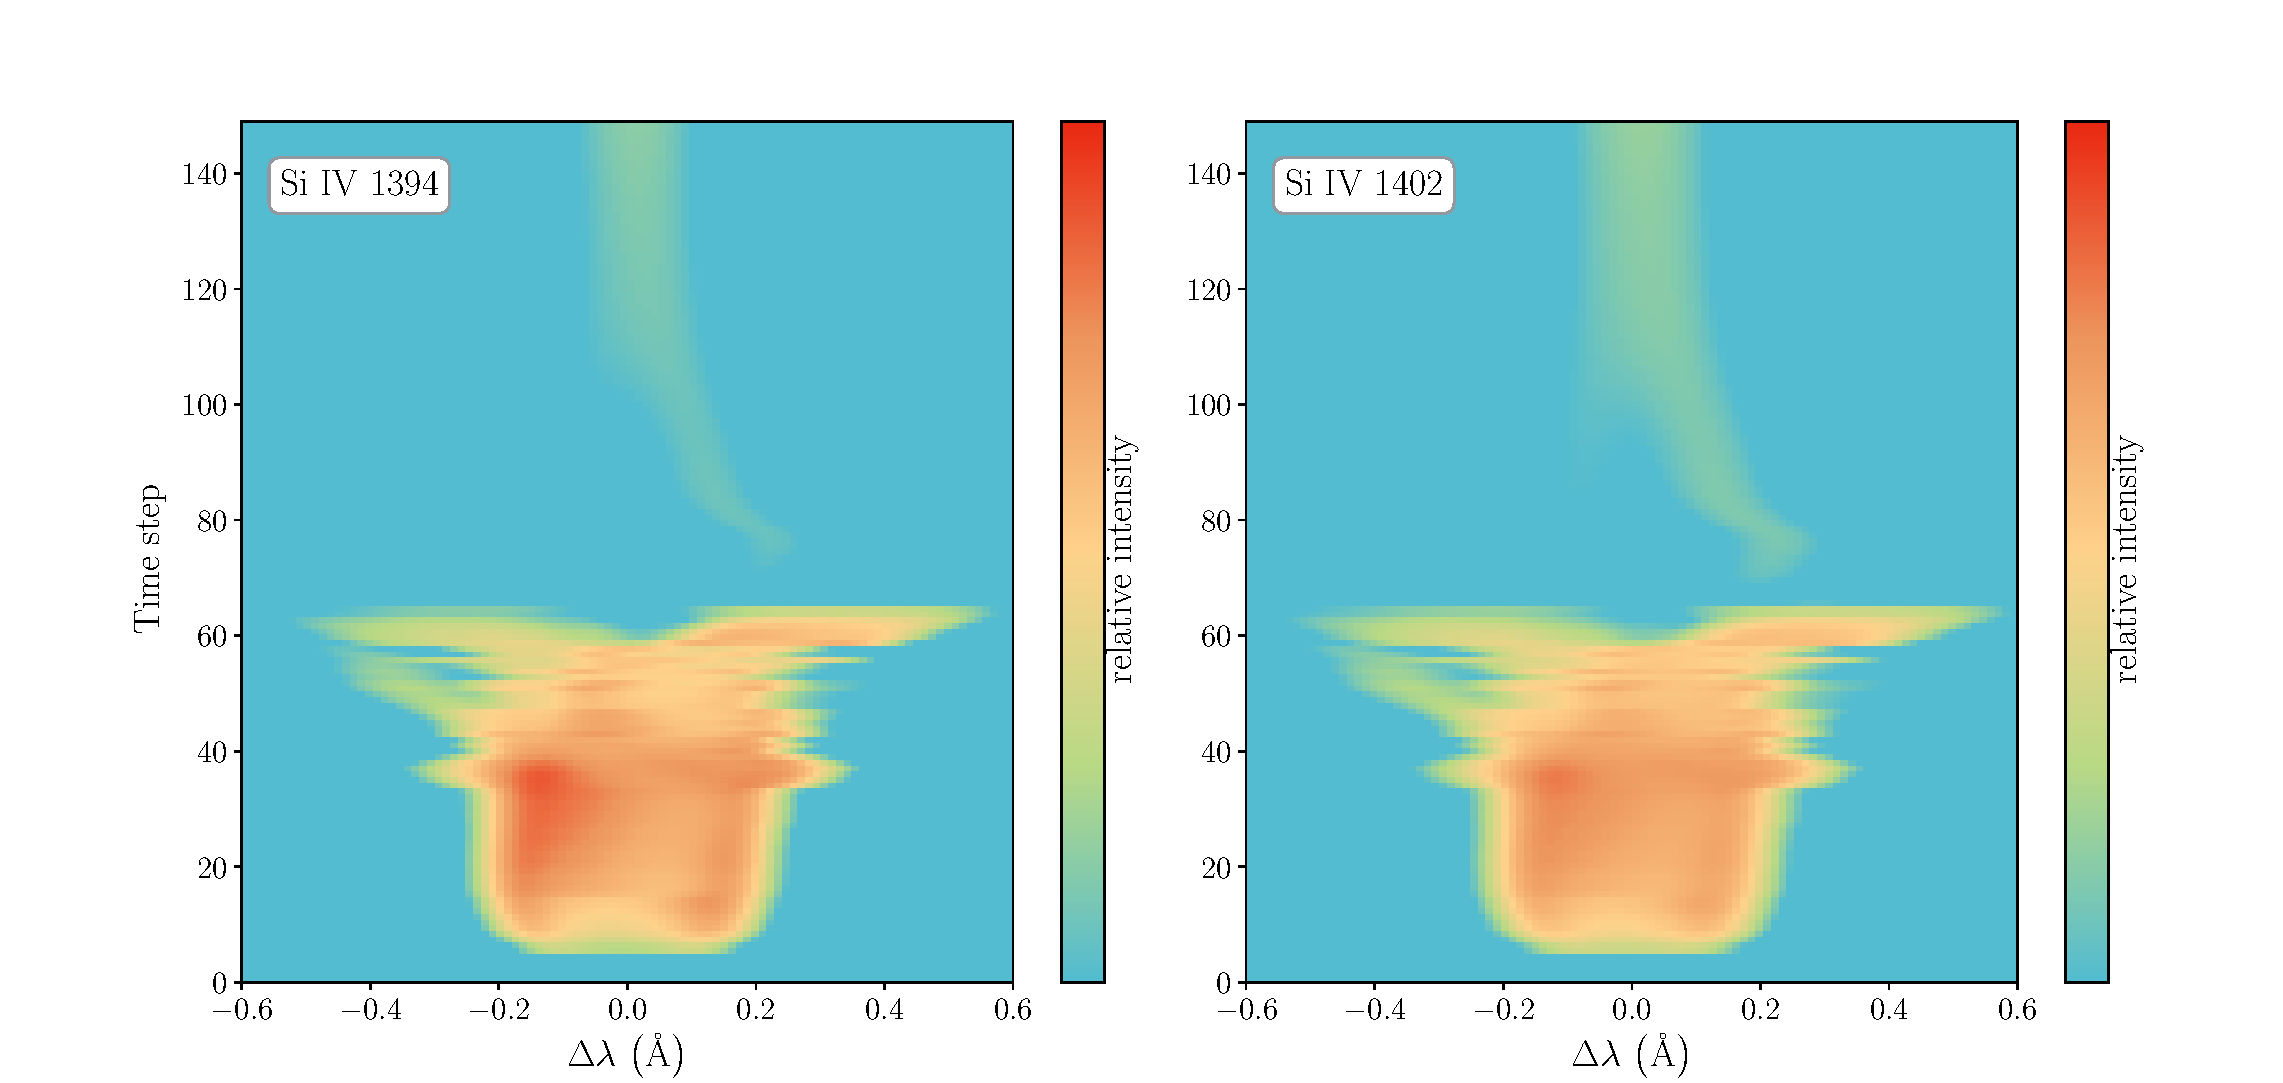
\includegraphics[width=\textwidth]{figs/5F11_spectra_imshow_Si}
	\caption{Si \textsc{iv}双重线强度随时间演化图,横坐标为波长,纵坐标为不同时刻,颜色代表该波长和时刻下的辐射强度。}
	\label{fig:3.8}
\end{figure}
我们在这一部分讨论Si \textsc{iv}双重线在光学厚辐射代码中合成光谱轮廓随时间演化的相关内容。近期有研究表明,Si \textsc{iv}双重线在耀斑爆发过程中可能是光学厚的\parencites{Kerr2019}。其中Si \textsc{iv}原子模型来源于基于RH的光学厚反演代码STiC\parencites{Rodriguez2016,Rodriguez2019},其原子模型是与RH代码相互兼容的。整个Si \textsc{iv}原子模型包含了5个Si III的能级和4个Si \textsc{iv}的能级(其中两个是Si \textsc{iv}的基态和连续态)。图~\ref{fig:3.8}展示了Si \textsc{iv}双重线内的辐射强度随着时间的演化,某些时刻的特征谱线轮廓展示在图~\ref{fig:3.9}中。
\begin{figure}
	\centering
	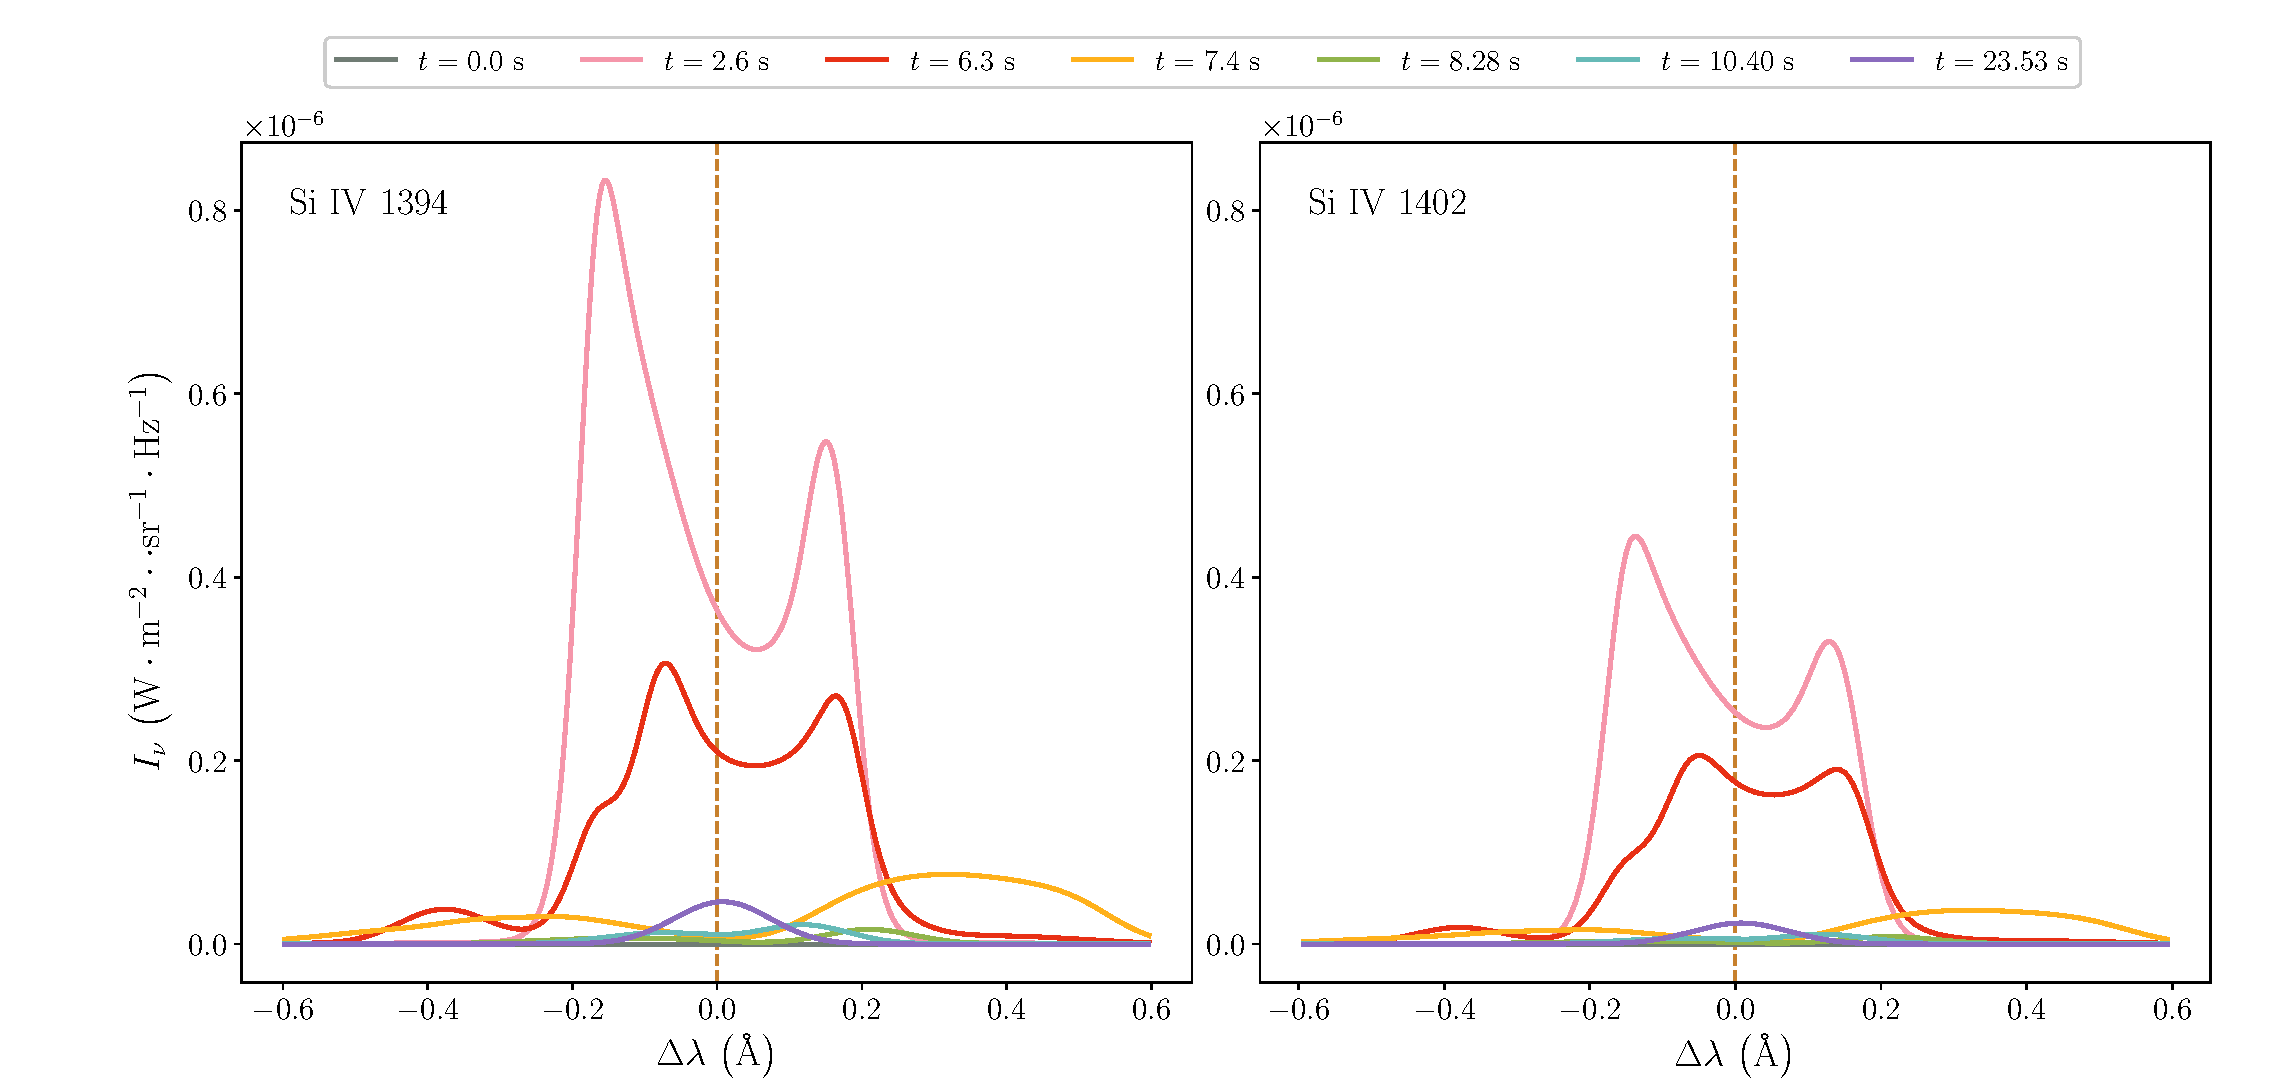
\includegraphics[width=\textwidth]{figs/5F11_spectra_line_Si}
	\caption{和图~\ref{fig:3.1}中时刻相近大气中计算得到的Si \textsc{iv}双重线谱线轮廓。}
	\label{fig:3.9}
\end{figure}

与C \textsc{ii}线相比,Si \textsc{iv}双重线的计算并没有出现数值问题。我们在计算时使用了一个比较大的微湍动速度$15\ \mathrm{km\  s^{-1}}$以再现Si \textsc{iv}形成在过渡区中的真实情况。具体的谱线演化与C \textsc{ii}线类似,一开始$t=2.6$ s线心反转的谱线的蓝侧峰不断增强,但是整个谱线的平分线速度(\textit{bisector velocity})并不大。随着加热的继续进行Si \textsc{iv}谱线的强度并没有继续增强,但是出现了一个小的蓝移分量($t=6.3$ s)。在$t=7.4$ s时,由于剧烈的色球凝聚和蒸发过程,谱线出现了一个很大的红移分量和一个比较小的蓝移分量。随着物质下流速度的逐渐减小,$t=8.28$ s和$t=10.40$ s时仅能看到一个相对较弱的红移分量。直到$t=23.53$ s时这个红移分量又逐渐回到静止波长位置,且辐射强度有一定程度的增强。



另外一个值得注意的变化是Si \textsc{iv}双重线的强度比,在光学薄极限下,两线强度比应该为2:1,在光学厚极限下则为1:1。从图~\ref{fig:3.9}中我们可以明显的看到,在模拟开始的时刻$t=2.6$ s和靠近结束的$23.53$ s,两线强度比似乎能够比较好地满足2:1的关系,而在某些时刻(如$t=6.3$ s),谱线的强度明显不符合这个关系,预示着此时的谱线的形成可能是光学厚的。为了能够更好地理解这两条谱线强度比在整个模拟过程中的演化,我们计算了两条线的积分强度随着时间的变化关系(见图~\ref{fig:3.10})。在耀斑发生一开始,两谱线比尚能维持在$1.8$左右,而当物质下流速度较大时($t>5$ s),两条谱线的强度比逐渐变小,当物质下流速度开始减小时($t\sim 7$ s),两条线的强度比又重新上升,一度到达2.0附近,但又很快重新下降,最后随着大气逐渐变得平静,两条谱线的强度比又重新向2.0移动。整个5F11模型中两线强度比的变化和\textcites{Kerr2019}中的结果相近,且进一步说明了在耀斑带上复杂的大气结构中,Si \textsc{iv}线可能形成在光学厚的环境中。

\begin{figure}
	\centering
	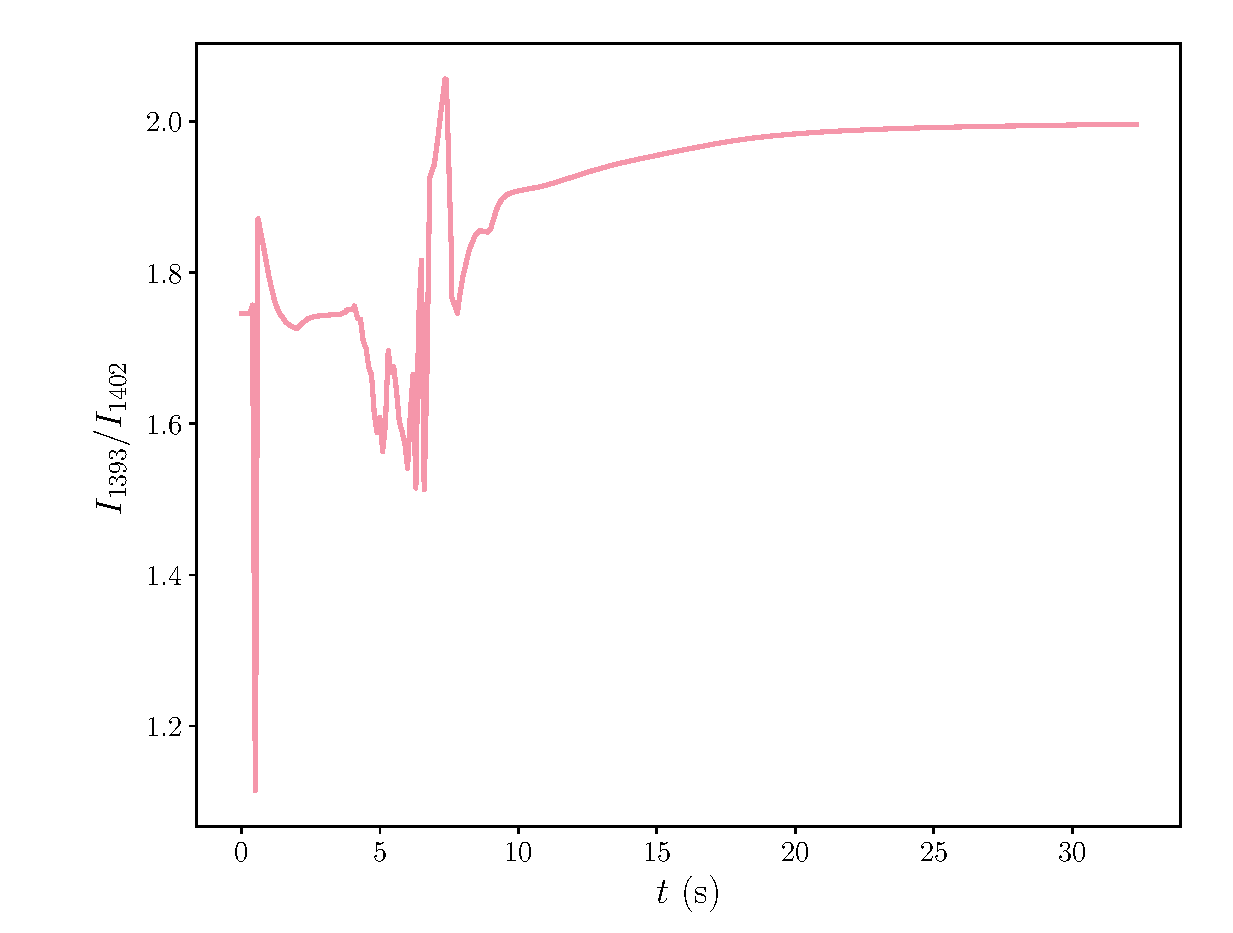
\includegraphics[width=0.6\textwidth]{figs/5F11_spectra_line_Si_ratio}
	\caption{Si \textsc{iv}双重线积分强度比随时间演化图。}
	\label{fig:3.10}
\end{figure}

同样的,基于Mg \textsc{ii}谱线在$t=23.53$ s与IRIS卫星观测比较匹配的结果,我们试图比较此时刻IRIS观测的Si \textsc{iv}双重线轮廓与合成光谱轮廓之间的关系。可以看到在IRIS观测中的谱线轮廓有着非常明显的红翼不对称性和一定的红移,而在$t=23.53$ s的Si \textsc{iv}则呈现出对称和几乎没有Doppler频移的特点。同时和C \textsc{ii}有着比较好拟合的$t=13.0$ s时的Si \textsc{iv}合成谱线则表现出一个蓝翼增强,和整个谱线轮廓更加不相符合。
\begin{figure}
	\centering
	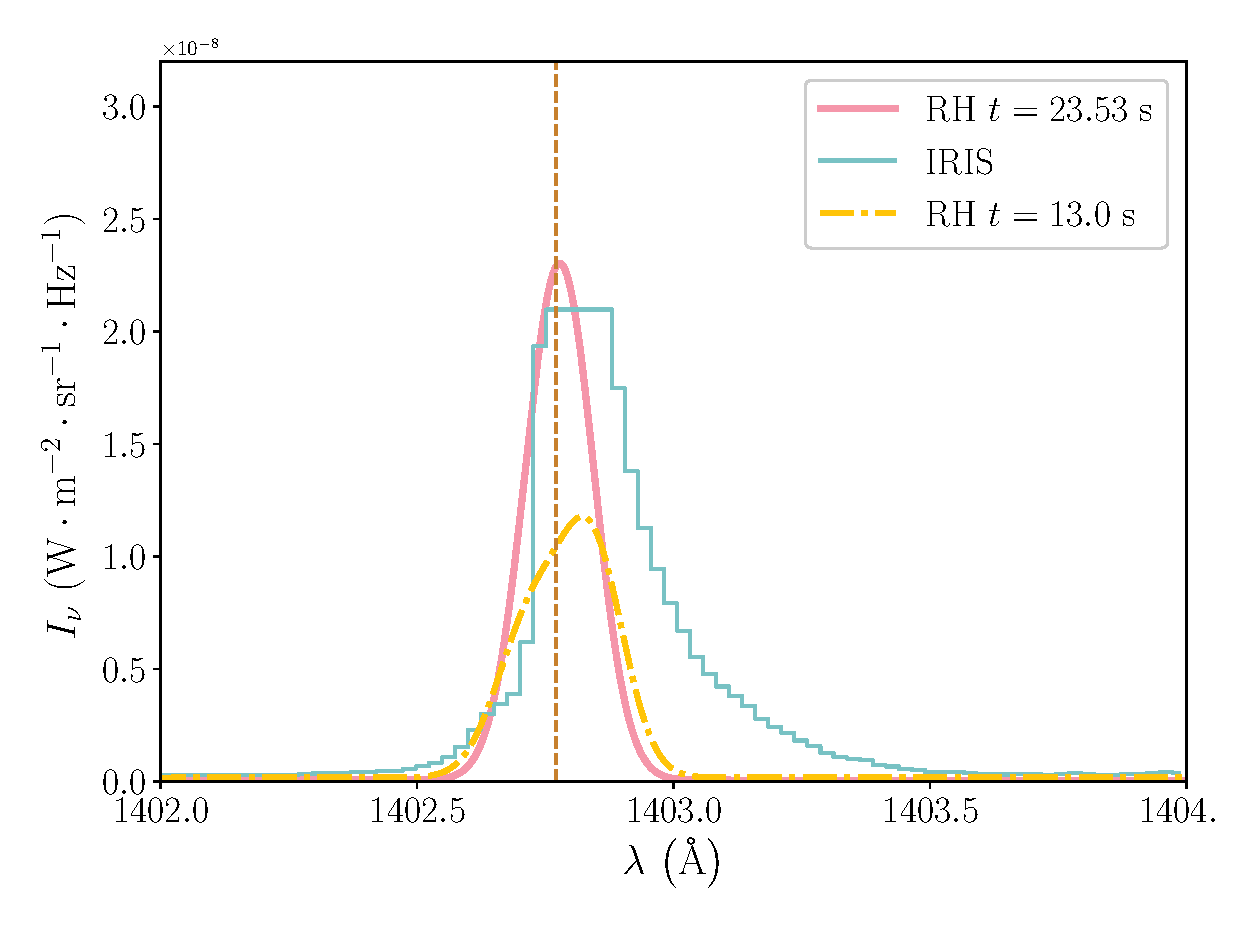
\includegraphics[width=0.7\textwidth]{figs/5F11_IRIS_SiIV}
	\caption{RH合成光谱中$t=13.0$ s和$t=23.53$ s时Si \textsc{iv}谱线轮廓与IRIS观测比较。由于IRIS此次观测没有Si \textsc{iv} 1393 \mbox{\AA}线的数据,我们仅比较了红翼的这条Si \textsc{iv}线,竖线代表了其静止波长。IRIS观测经过辐射定标之后被乘以了一个5的因子使的其强度能够与合成光谱相比较。}
\end{figure}
\section{谱线形成分析}\label{sec:3.7}
最后我们通过\ref{sec:1.2.2}节中描述的贡献函数方法来分析一些和观测拟合比较好的谱线轮廓的形成高度和对应一些大气参数。首先是拟合比较好的Mg \textsc{ii}线,首先我们在图~\ref{fig:3.11}中对比了一个有较明显线心反转和一个几乎没有线心反转的谱线轮廓。可以看到合成光谱中Mg \textsc{ii}线心是否出现线心反转是和线心形成高度的电子密度密切相关的。

图~\ref{fig:3.11}中左侧的线心反转谱线形成在$t=10.0$ s处,由于色球层已经被压缩,整个线心形成高度只有大约$142$ m。由于形成于平均速度下流为$\sim36\ \mathrm{km\  s^{-1}}$的区域,谱线有明显的红移。线心形成位置温度约为$\sim 1.5\times10^4$ K,电子密度约为$5.84\times10^{14}\ \mathrm{cm^{-3}}$。由于电子密度相对较小,原函数$S_\nu$在线心形成高度上和Planck函数$B_\nu$有较大差距,因此线心处的辐射不足,产生了线心反转。而右侧的位于$t=27.56$ s的谱线轮廓,由于此时线心形成位置的体速度只有$\sim 5\ \mathrm{km \  s^{-1}}$,因此此时的谱线红移较小。与之前线心反转的谱线相比,此时的谱线形成高度的平均电子密度较大,达到了$\sim 7.8\times10^{14}\ \mathrm{cm^{-3}}$。较高的电子密度保证了线心形成在近似LTE的位置,有足够的辐射强度产生单发射峰。

由此我们也可以简单解释为什么图~\ref{fig:3.3.5}中较小$\mu = 0.2$下的Mg \textsc{ii}谱线轮廓会更宽且有更加明显的线心反转。由于$\mu$较小,说明视线方向与平面平行层大气的法线方向夹角越大,此时我们看到的是与$\mu=0.77$相比从大气更高部分发出的光子。那里的线翼形成高度电子密度更大,线心部分源函数$S_\nu$与Planck函数$B_\nu$的脱耦更明显,因此谱线更宽但线心反转更明显。


\begin{figure}[htbp]
	\begin{minipage}[t]{0.5\linewidth}
	\centering
	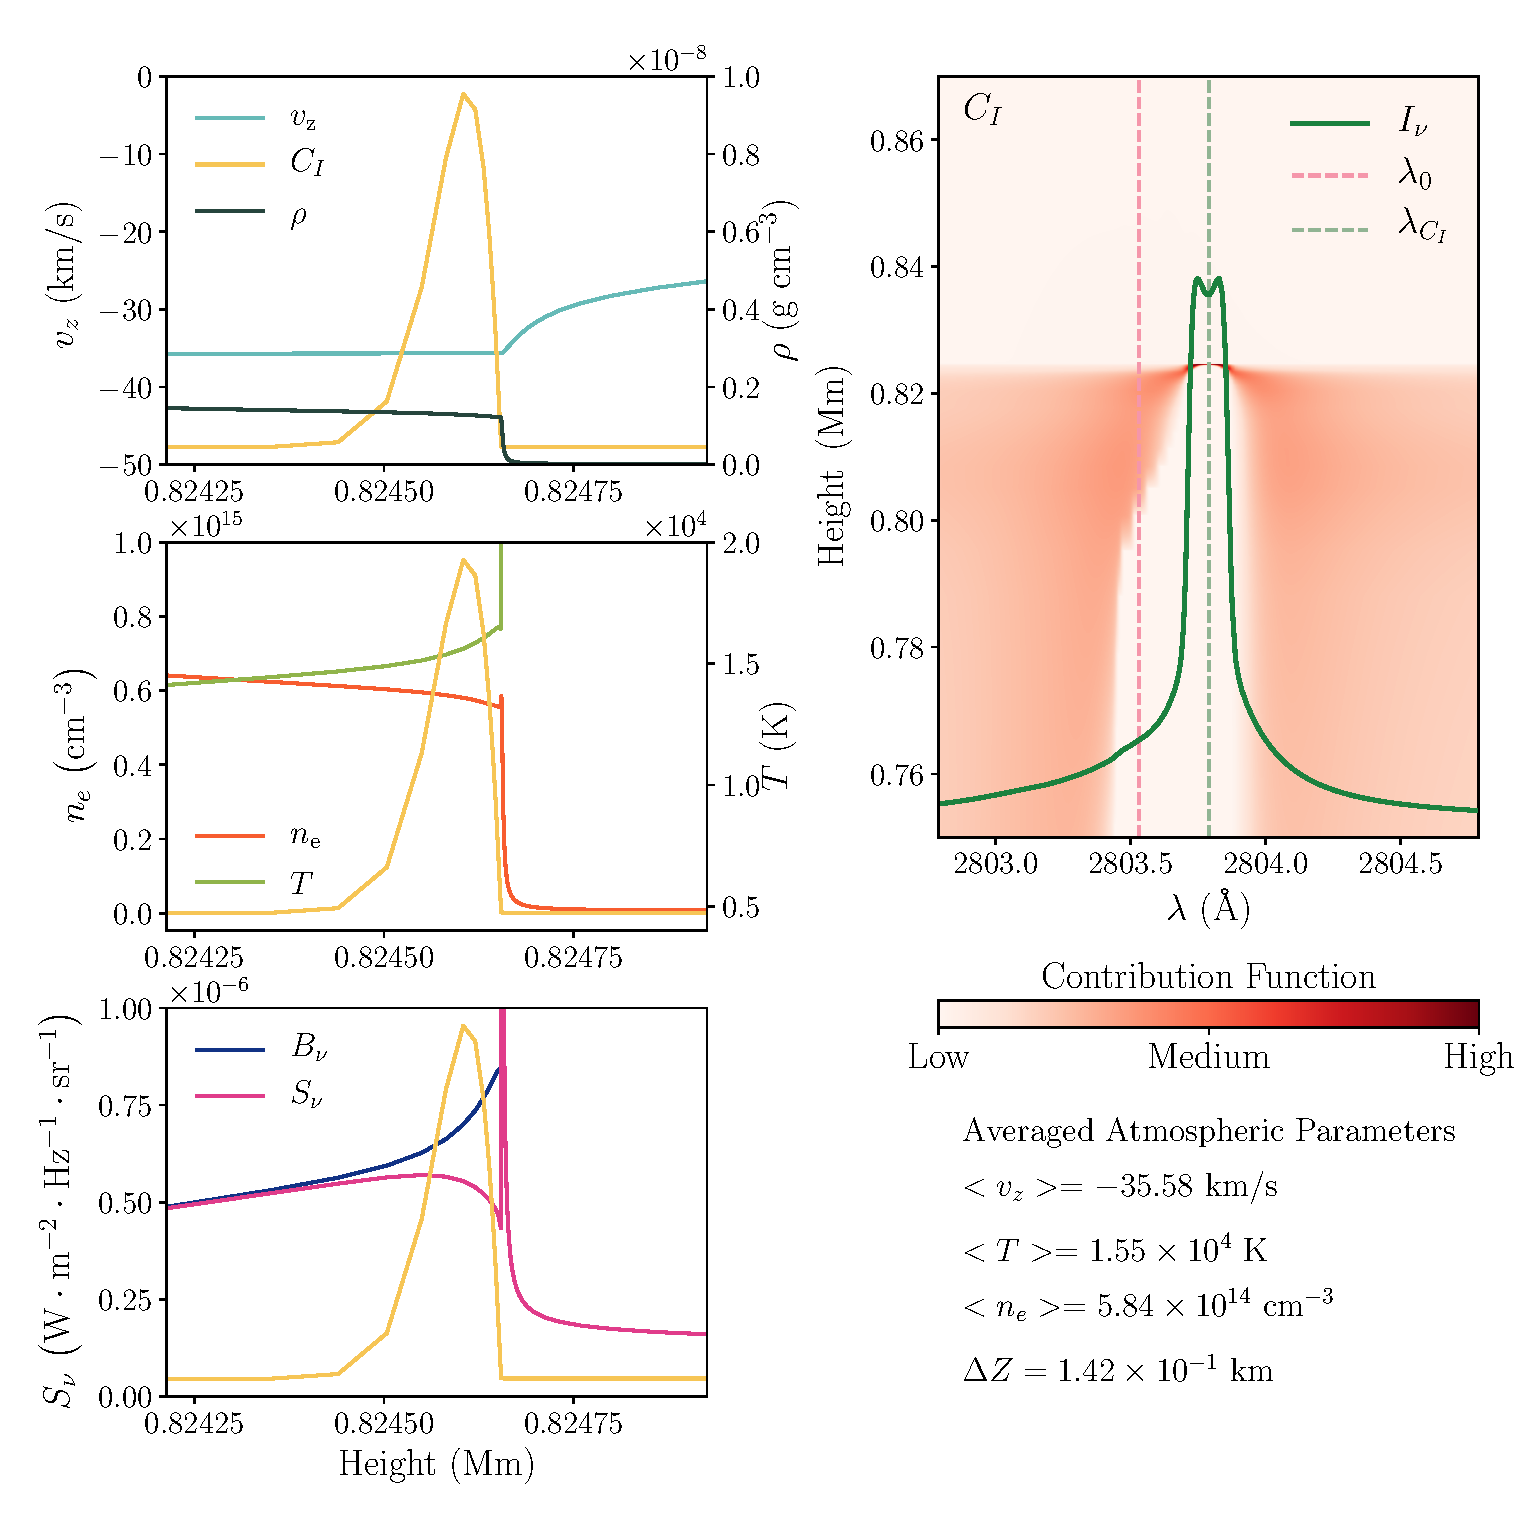
\includegraphics[width=\linewidth]{figs/ctb_5F11_88_lc}
	\end{minipage}%
	\hfill
	\begin{minipage}[t]{0.5\linewidth}
	\centering
	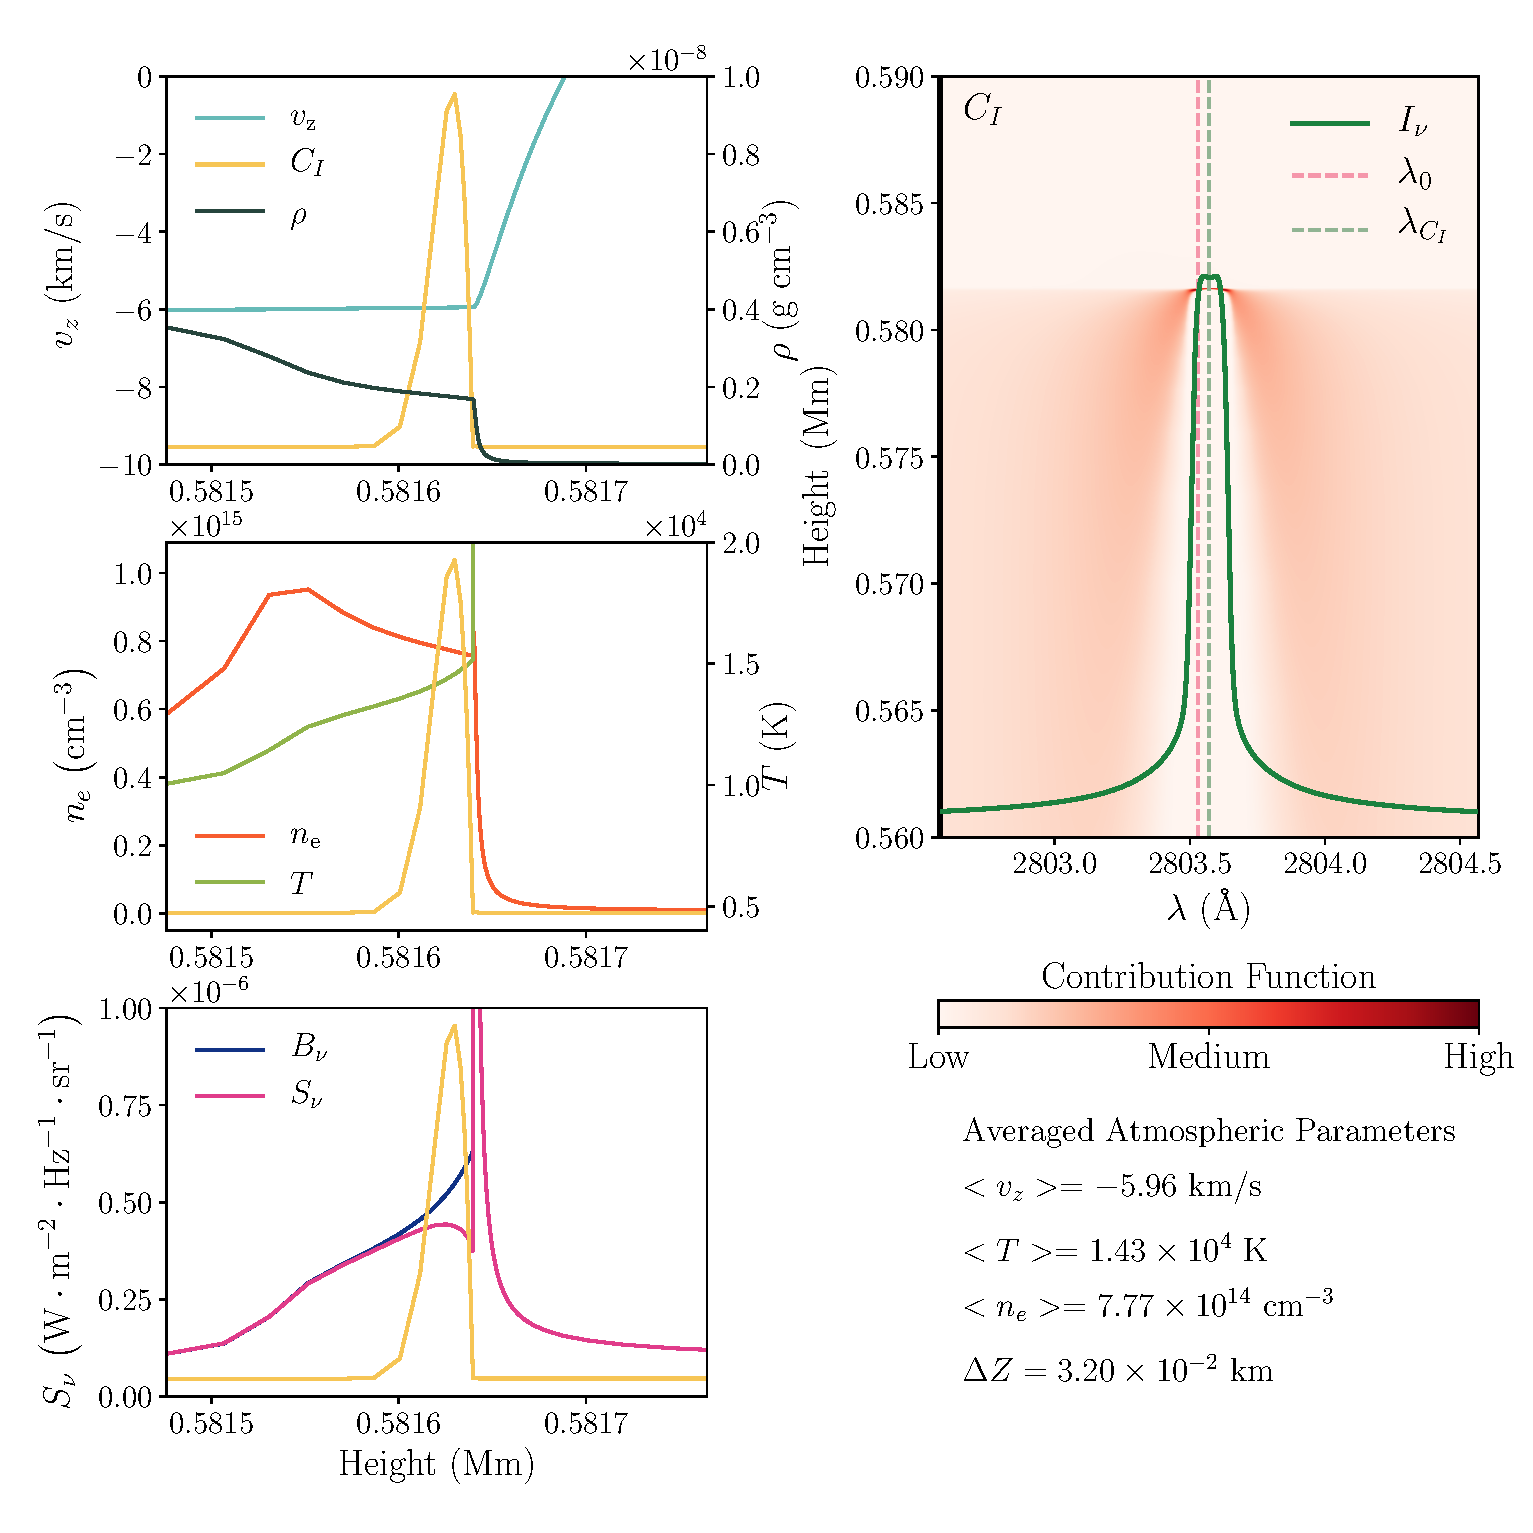
\includegraphics[width=\linewidth]{figs/ctb_5F11_250_lc}
	\end{minipage}
	\caption{左:$t=10$ s时Mg \textsc{ii} h线的贡献函数分析;右:$t=27.56$ s时Mg \textsc{ii} h线的贡献函数分析。每个图中的内容是:左上——一维速度、密度、$\lambda_c$处贡献函数随高度分布;左中——温度和电子密度随高度分布;左下——源函数和Planck函数随高度分布;右上——谱线轮廓与贡献函数在频率和波长上的分布;右下——以贡献函数作为权重函数对形成区域内的大气参数的加权平均。}
	\label{fig:3.11}
\end{figure}

\begin{figure}[htbp]
	\begin{minipage}[t]{0.5\linewidth}
	\centering
	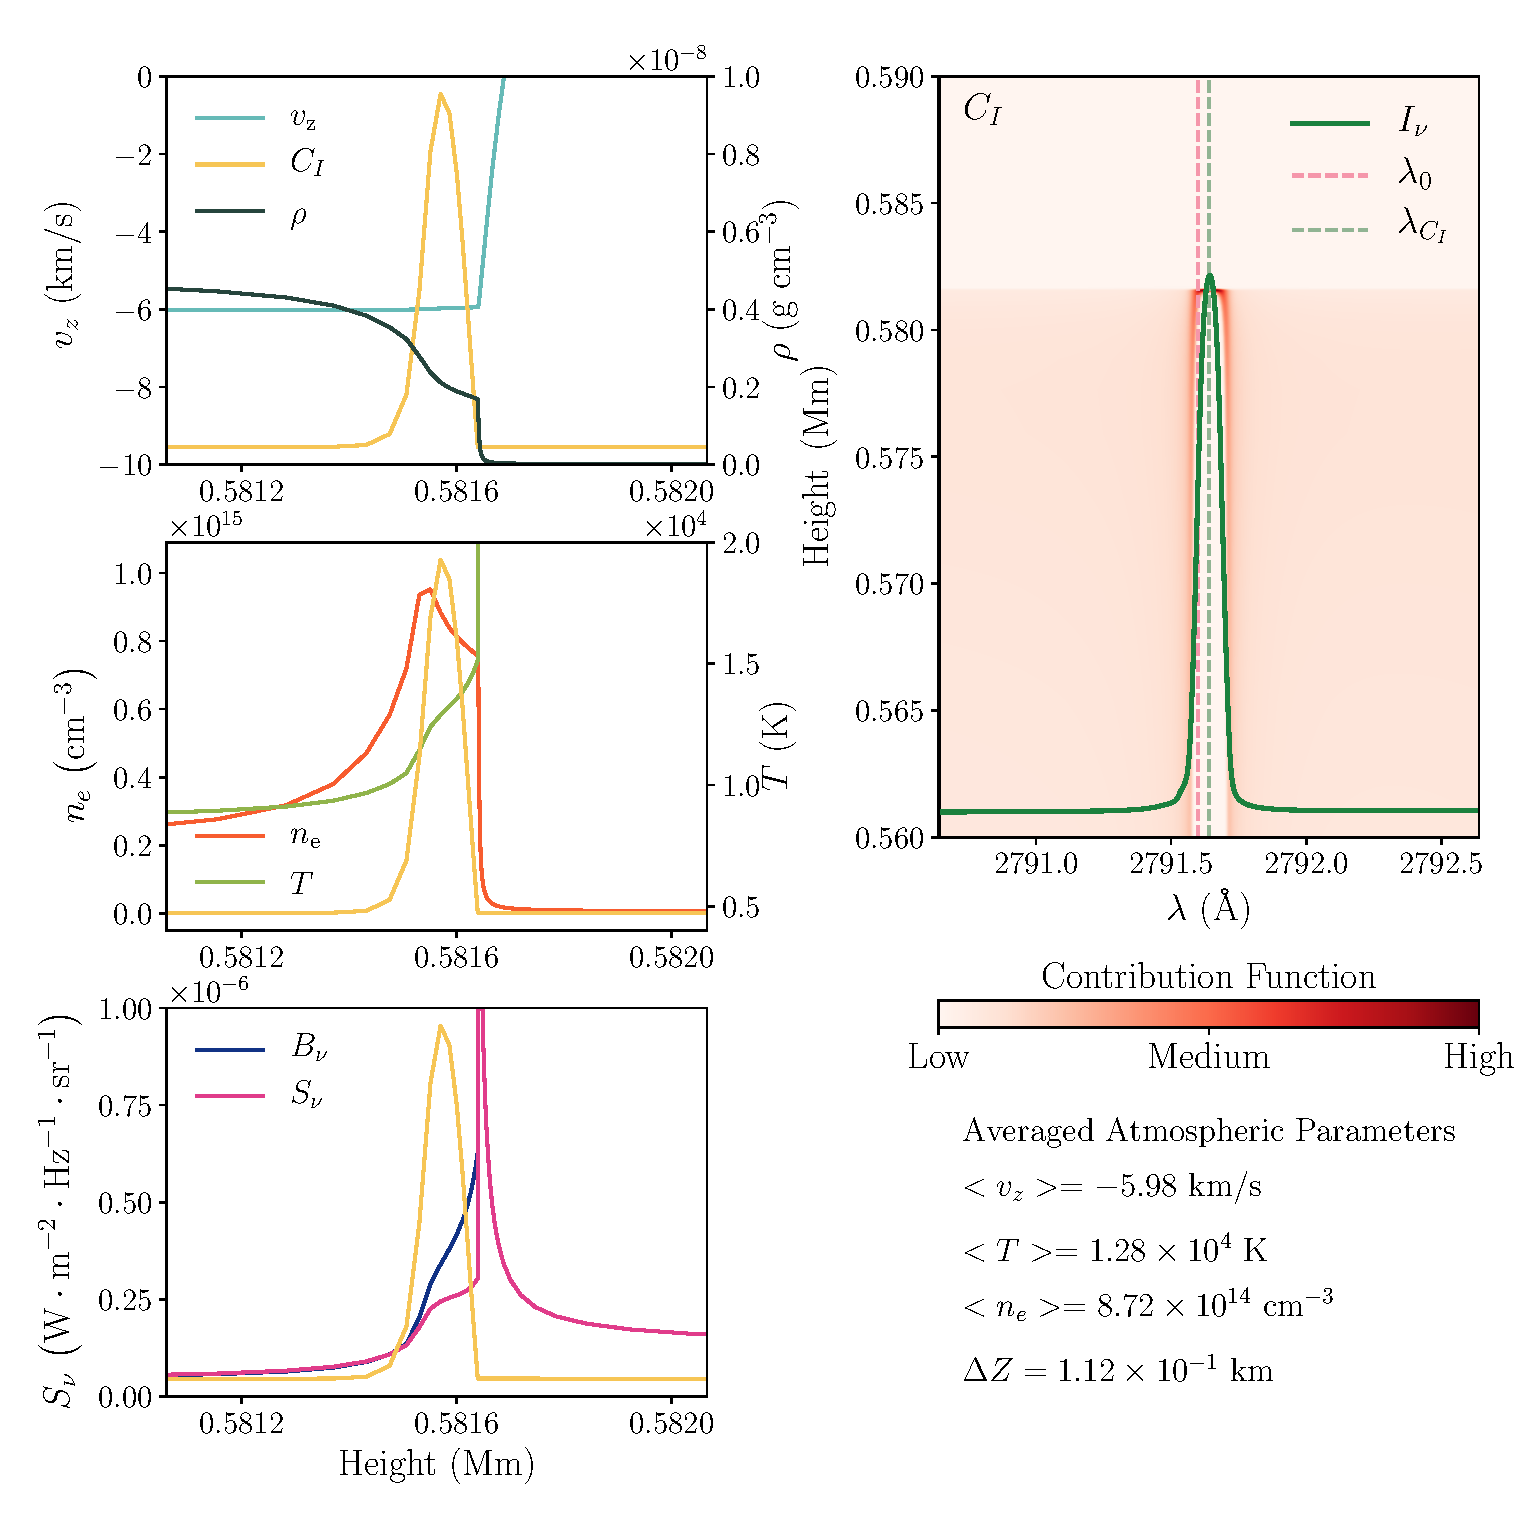
\includegraphics[width=\linewidth]{figs/ctb_5F11_250_lc_2}
	\end{minipage}%
	\hfill
	\begin{minipage}[t]{0.5\linewidth}
	\centering
	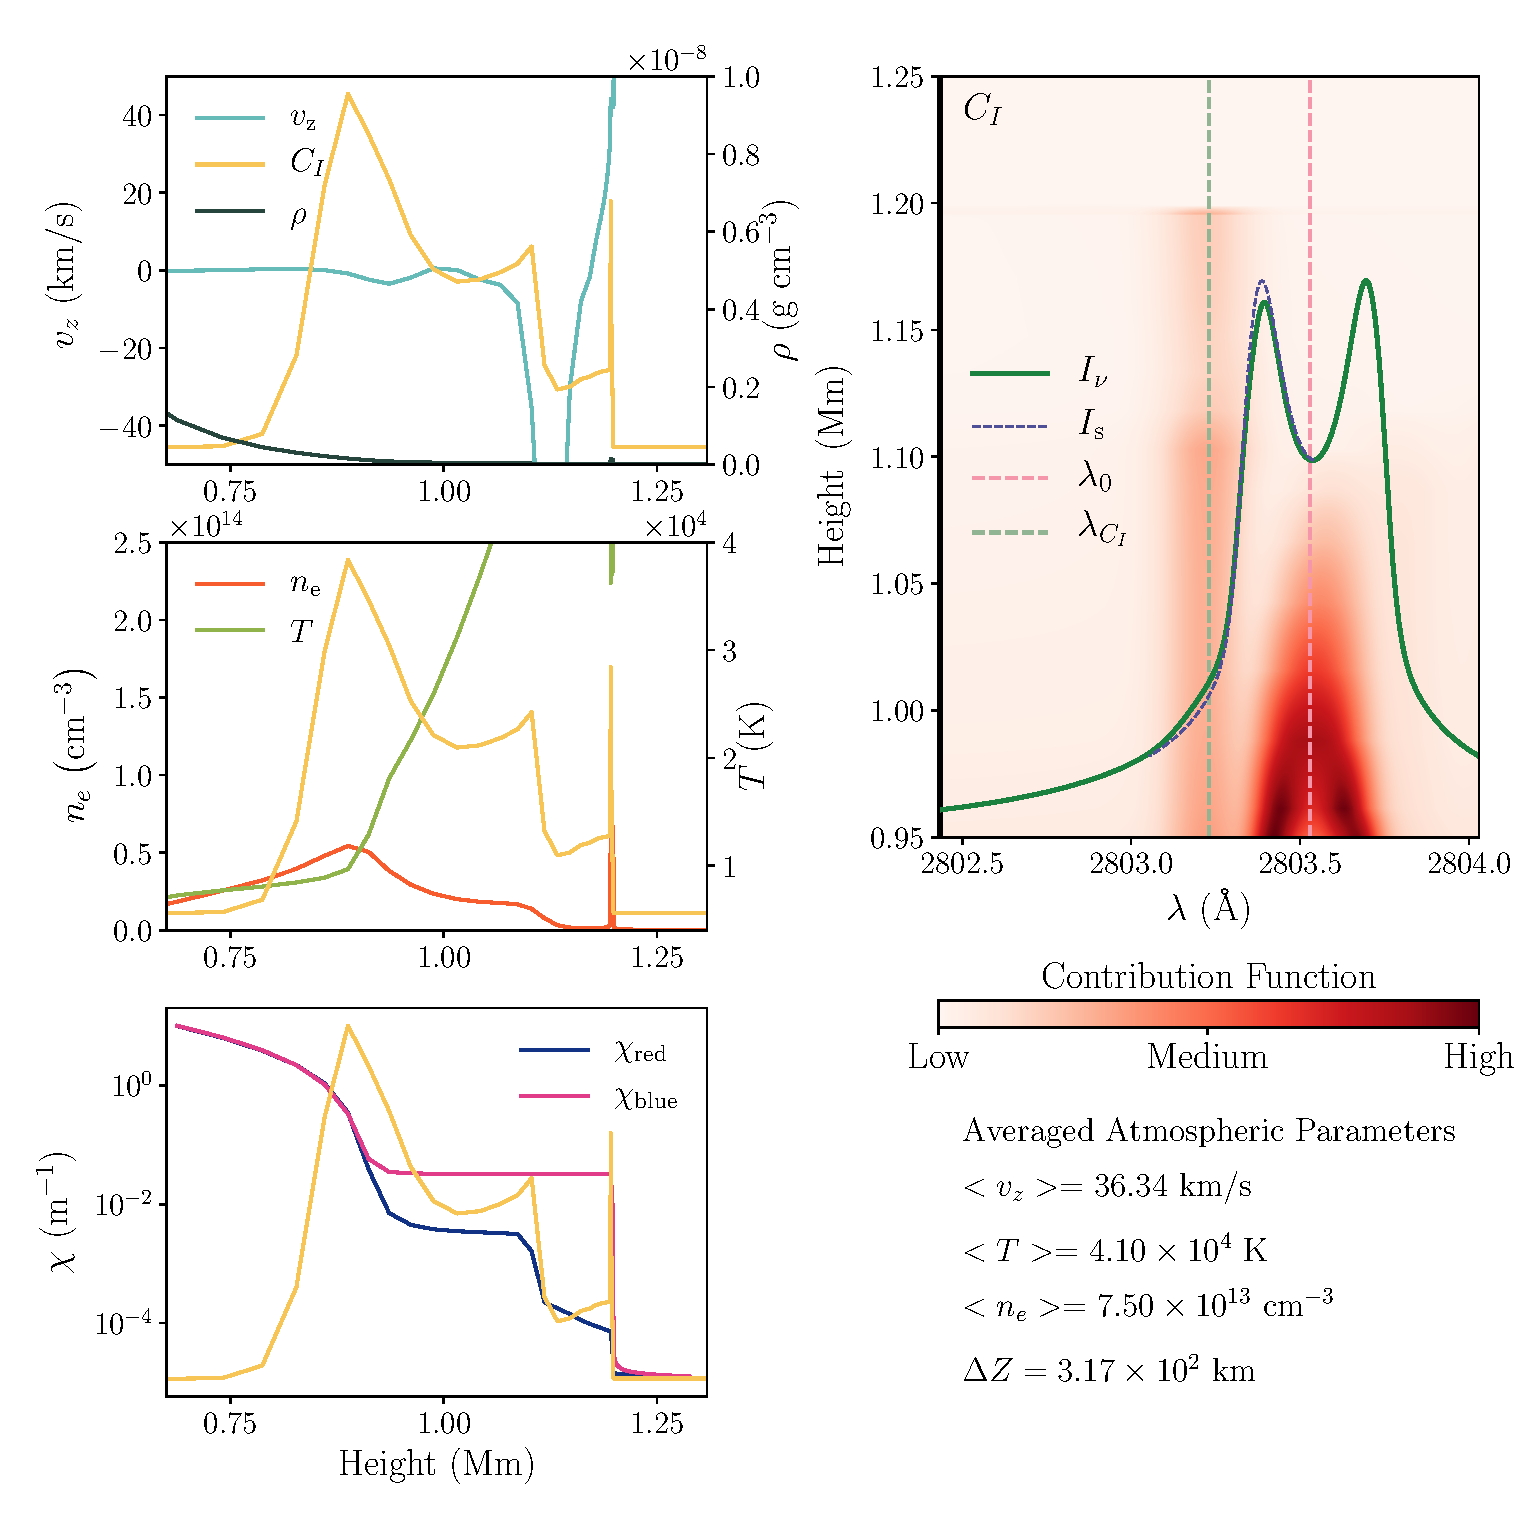
\includegraphics[width=\linewidth]{figs/ctb_5F11_44}
	\end{minipage}
	\caption{左:$t=27.56$ s时Mg \textsc{ii} 2791 \mbox{\AA}线的贡献函数分析;右:$t=5.30$ s时在RH+SB$\times$30中计算的Mg \textsc{ii} h线的贡献函数分析。其平均大气参数是在上流的冷物质部分求的平均。}
	\label{fig:3.12}
\end{figure}

图~\ref{fig:3.12}左栏展示了和图~\ref{fig:3.11}中非线心反转Mg \textsc{ii} h线同时的Mg \textsc{ii} 2791 \mbox{\AA}线,通过对其线心形成高度的分析,我们发现其生成在和Mg \textsc{ii} h线非常相近的高度上。这也解释了为什么我们在\ref{sec:3.4}节中对Mg \textsc{ii} h和k线线心形成高度的微湍动速度进行进一步调整时,Mg \textsc{ii}三重线也会剧烈致宽。

图~\ref{fig:3.12}右栏展示了$t=5.30$ s一个具有微弱蓝翼不对称性的Mg \textsc{ii} h谱线轮廓,我们使用了RH+SB$\times$30代码来计算谱线轮廓使其线翼辐射能够和实际观测相比。对蓝翼增强位置的贡献函数分析表明,这一增强来自于一个冷的物质上流提高了这一波长位置的不透明度。这团上流物质的特征温度约为$\sim4\times10^4$ K,速度约为$\sim 36\ \mathrm{km\  s^{-1}}$,电子密度约为$7.5\times10^{13}\ \mathrm{cm^{-3}}$。

\begin{figure}[htbp]
	\begin{minipage}[t]{0.5\linewidth}
	\centering
	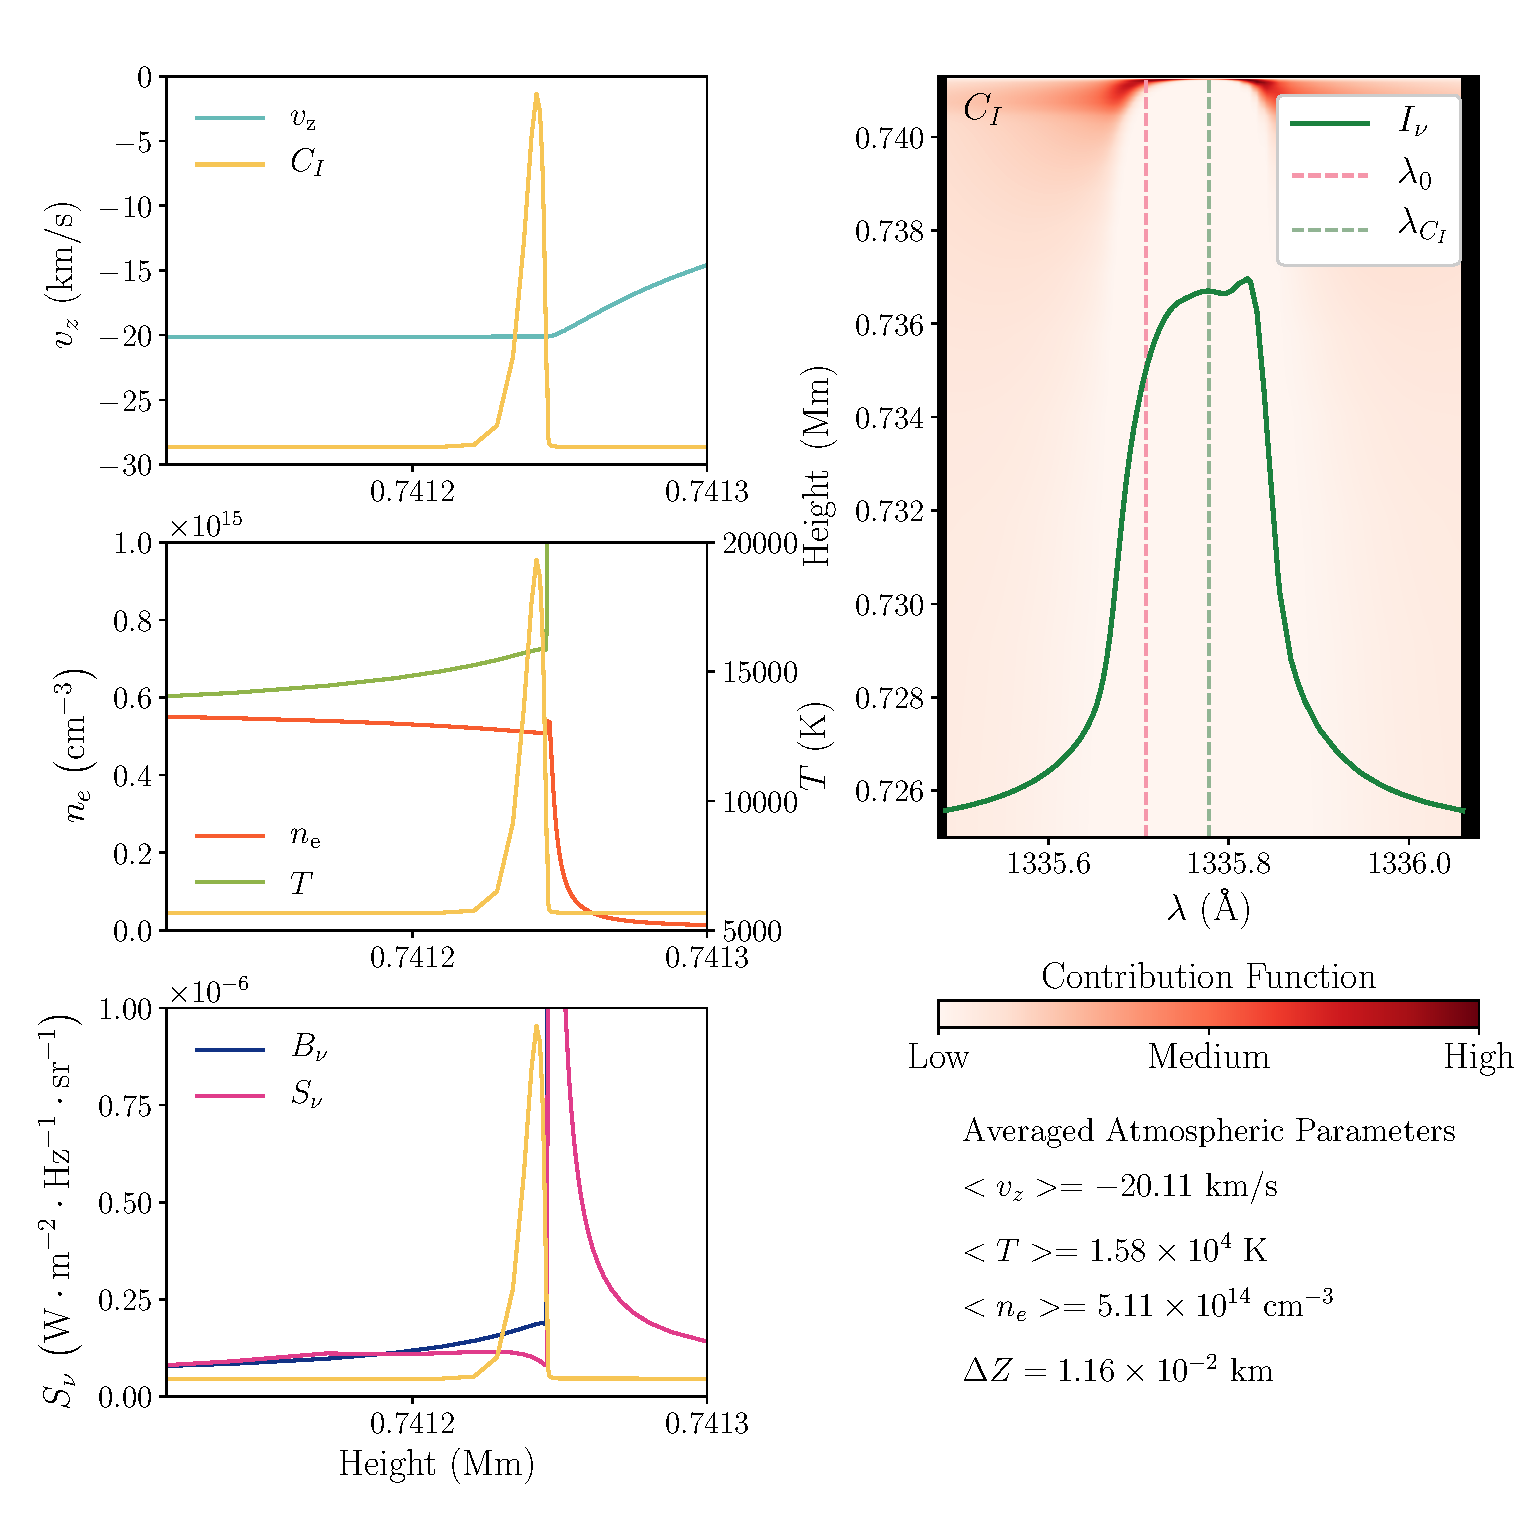
\includegraphics[width=\linewidth]{figs/ctb_5F11_112_CII}
	\end{minipage}%
	\hfill
	\begin{minipage}[t]{0.5\linewidth}
	\centering
	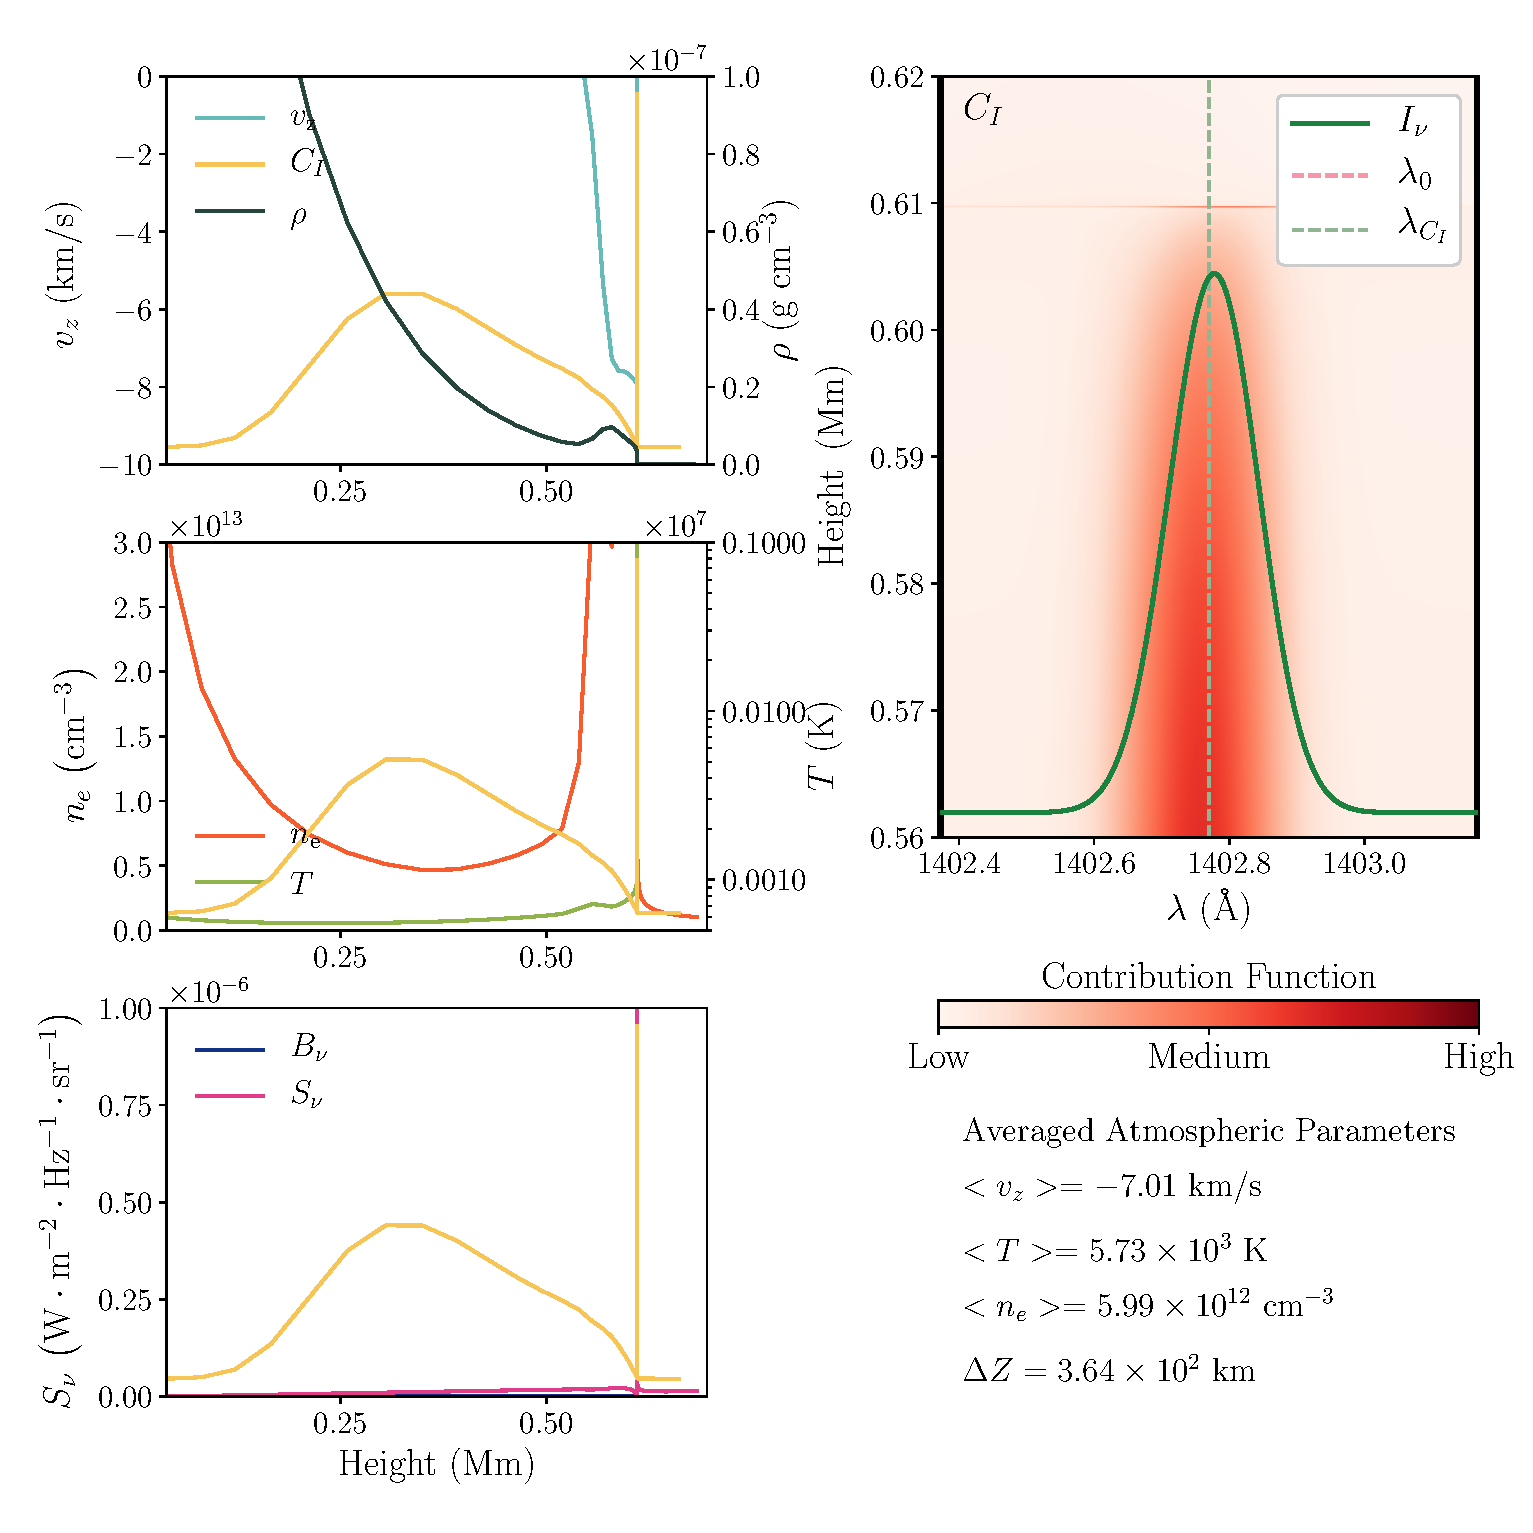
\includegraphics[width=\linewidth]{figs/ctb_5F11_SiIV_210}
	\end{minipage}
	\caption{左:$t=13.0$ s时C \textsc{ii} 1335 \mbox{\AA}线的贡献函数分析;右:$t=23.53$ s时Si \textsc{iv} 1402 \mbox{\AA}线的贡献函数分析。}
	\label{fig:3.13}
\end{figure}


之后我们来分析和观测符合得不太好的C \textsc{ii}和Si \textsc{iv}线。图~\ref{fig:3.13}左栏展示了$t=13.0$ s与IRIS观测在红移上拟合比较好的C \textsc{ii}线。从谱线形成高度上来看,C \textsc{ii}线的形成高度基本和Mg \textsc{ii}线重合,略高约数公里。但是C \textsc{ii}线线心形成区域受色球压缩的影响更强,其线心形成范围只有$\sim 11$ m,紧贴在过渡区下面。形成高度上的温度约为$\sim1.6\times10^4$ K,电子密度约为$\sim 5.1 \times 10^{14}\ \mathrm{cm^{-3}}$。

图~\ref{fig:3.13}右栏中展示的是Si \textsc{iv}线在$t=23.53$ s时谱线轮廓和贡献函数分析,值得注意的是这里Si \textsc{iv}线心除了一个位于过渡区的明显贡献之外,还存在着大量来自色球的贡献,因此说明此时的合成光谱是不太可靠的。我们将在之后\ref{sec:3.8}节中的讨论中分析为什么RH代码在此时计算Si \textsc{iv}谱线轮廓出现了问题。
\section{He \textsc{i} 10830 \mbox{\AA}线的Stokes参数变化}
在最后我们想尝试通过RH代码支持的计算整个谱线的Stokes参数的辐射转移的功能。He \textsc{i} 10830 \mbox{\AA}三重线是位于近红外的三条重要发射线,他们的空气波长为10829.09 \mbox{\AA},10830.250 \mbox{\AA}和10830.34 \mbox{\AA},真空波长为10832.06 \mbox{\AA},10833.22 \mbox{\AA}和10833.31 \mbox{\AA}。分别来自于能级$1s2p\ ^3P_0-1s2s\ ^3S_1$,$1s2p\ ^3P_1-1s2s\ ^3S_1$和$1s2p\ ^3P_2-1s2s\ ^3S_1$的跃迁。它们一般形成在高色球区域,离日冕约$\sim 2$ Mm的位置\parencites{Avrett1994,Chaouche2012}。目前对其的形成高度和谱线轮廓等尚未有较为详细的辐射流体力学模拟研究,但在具体观测中已经被广泛地用于色球磁场的测量中。特别是在耀斑带上,近期\textcites{Libbrecht2019}利用10830线和He \textsc{i} $D_3$线研究了耀斑带上的磁场强度,认为耀斑带上有大约$\sim 2500$ G的磁场。而\textcites{Anan2018}对一个C级耀斑耀斑带上的He \textsc{i} 10830 \mbox{\AA}的Stokes参数进行了观测,并利用弱场近似得到了耀斑带上大约有$\sim 1000$ G左右的磁场。

目前尚没有能够对He \textsc{i} 10830线进行高空间和光谱分辨率观测的望远镜和仪器。但随着下一代太阳望远镜-拥有4 m主镜的Daniel K. Inouye太阳望远镜(\textit{DKIST}, \cites{DKIST2014})的建成,其所搭载的衍射极限近红外分光偏振计(\textit{Diffraction Limited Near Infrared Spectropolarimeter, DL-NRISP}: \cites{DKIST2007})将使用He \textsc{i} 10830 \mbox{\AA}作为用于测量太阳色球磁场的重要谱线之一。整个DL-NRISP将以前所未有的空间分辨率(最高至0.5个角秒)和光谱分辨率($R\sim 250000$)同时测量Stokes $I$,$Q$,$U$,$V$四个参数。届时,He \textsc{i} 10830 \mbox{\AA}肯定会在太阳色球磁场测量中发挥相当重要的作用。

基于这样的考虑,我在RH的大气输入模型中手动插入了一个$B_z = 500$ G的磁场,然后计算He \textsc{i} 10830 \mbox{\AA}谱线内的I,Q,U,V四个参数的辐射转移。图~\ref{fig:3.14}展示了整个过程中的Stokes参数随时间的演化。我们另在图~\ref{fig:3.15}中展示了一些特征时间的Stokes参数轮廓。可以看出整个He \textsc{i} 10830 \mbox{\AA}线由于形成在高色球,因此也和Mg \textsc{ii} h等线一样在电子束加热大气产生色球凝聚时产生比较大的红移,随后不断减小。谱线的线偏振度和圆偏振度都在耀斑加热相达到极值。其中代表圆偏振度的的Stokes $V/I$大约在5\%-15\%的量级,比\textcites{Anan2018}对C级耀斑的观测结果稍大。
\begin{figure}
	\centering
	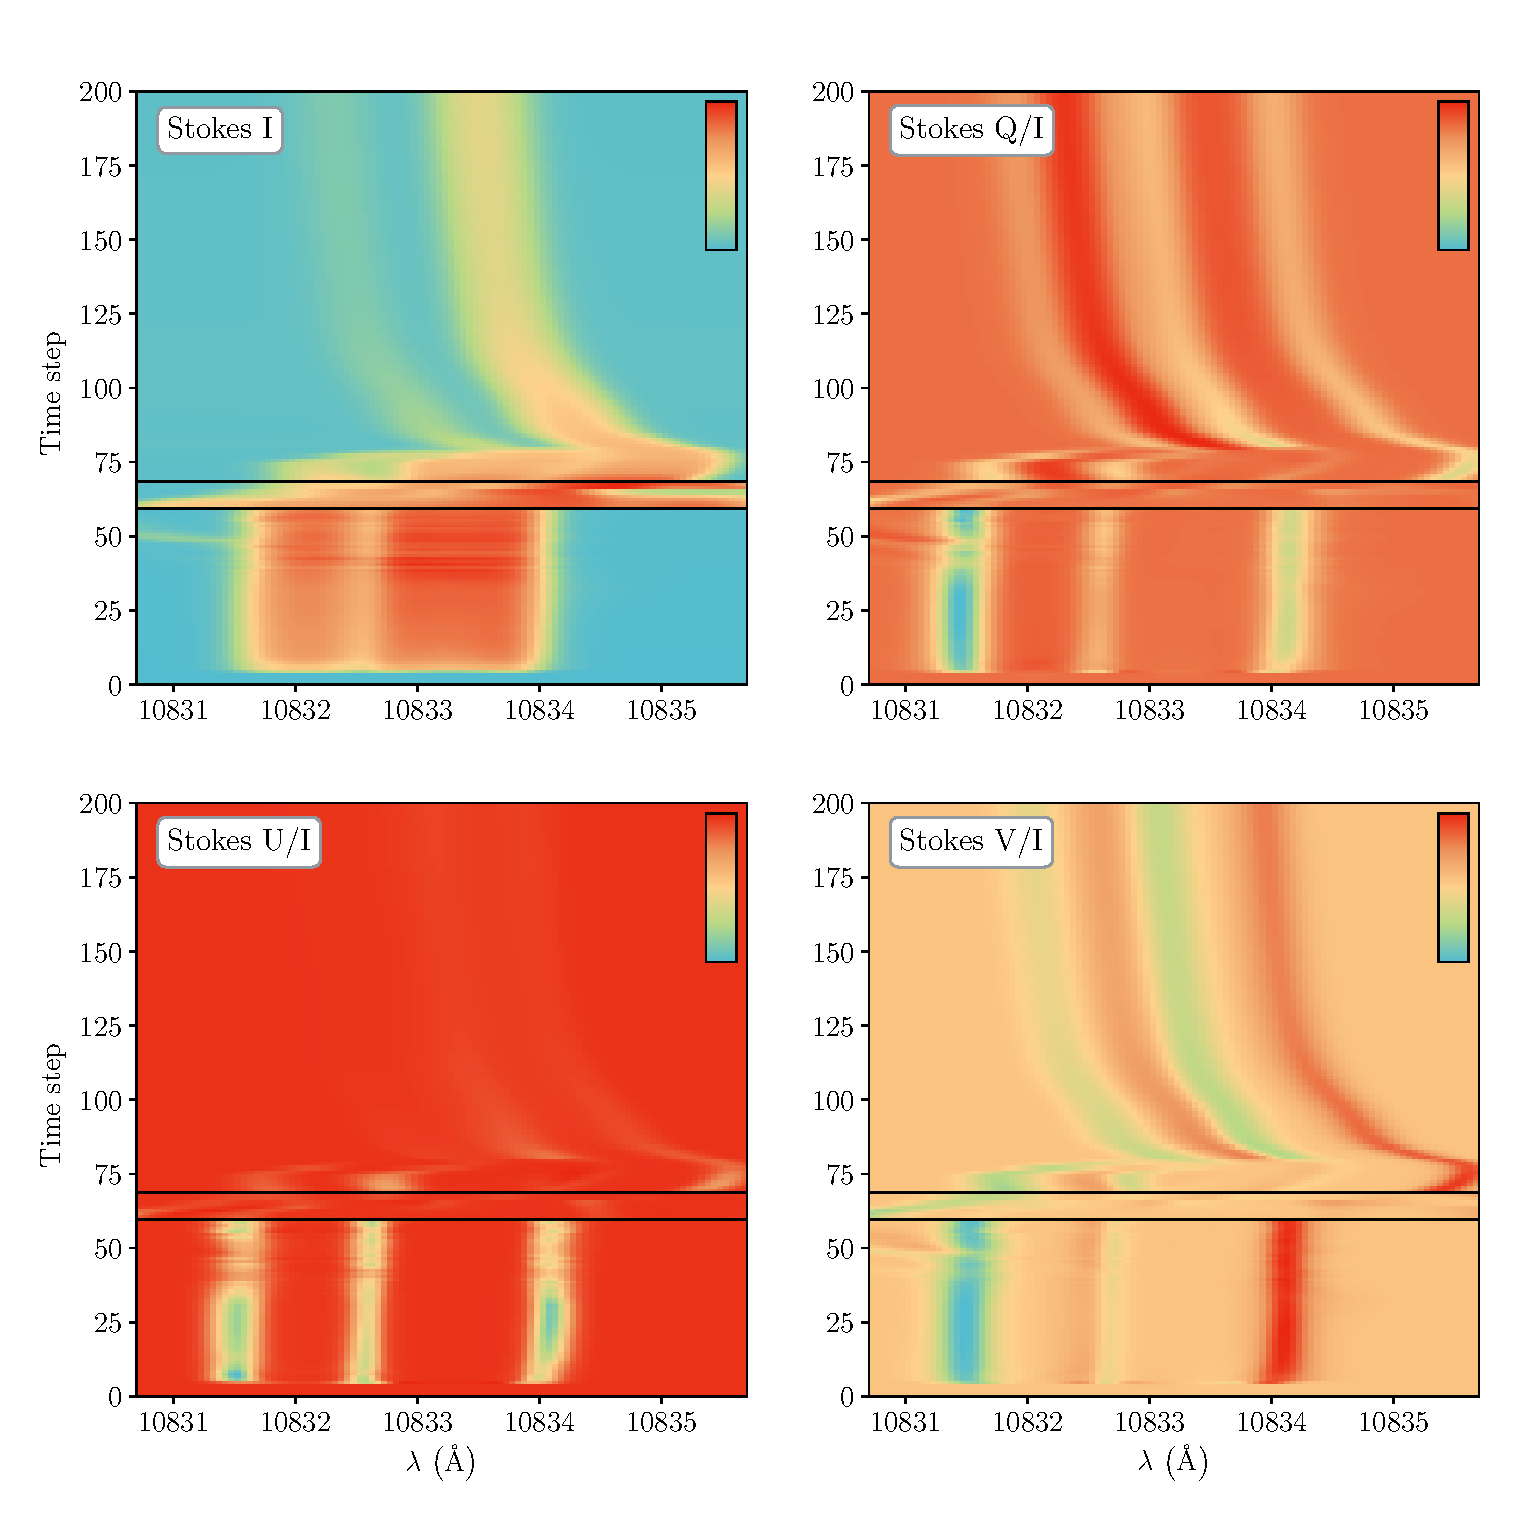
\includegraphics[width=0.6\textwidth]{figs/HeI_Stokes_imshow}
	\caption{He \textsc{i} 10830 \mbox{\AA}线Stokes参数在模拟中的演化。}
	\label{fig:3.14}
\end{figure}

\begin{figure}
	\centering
	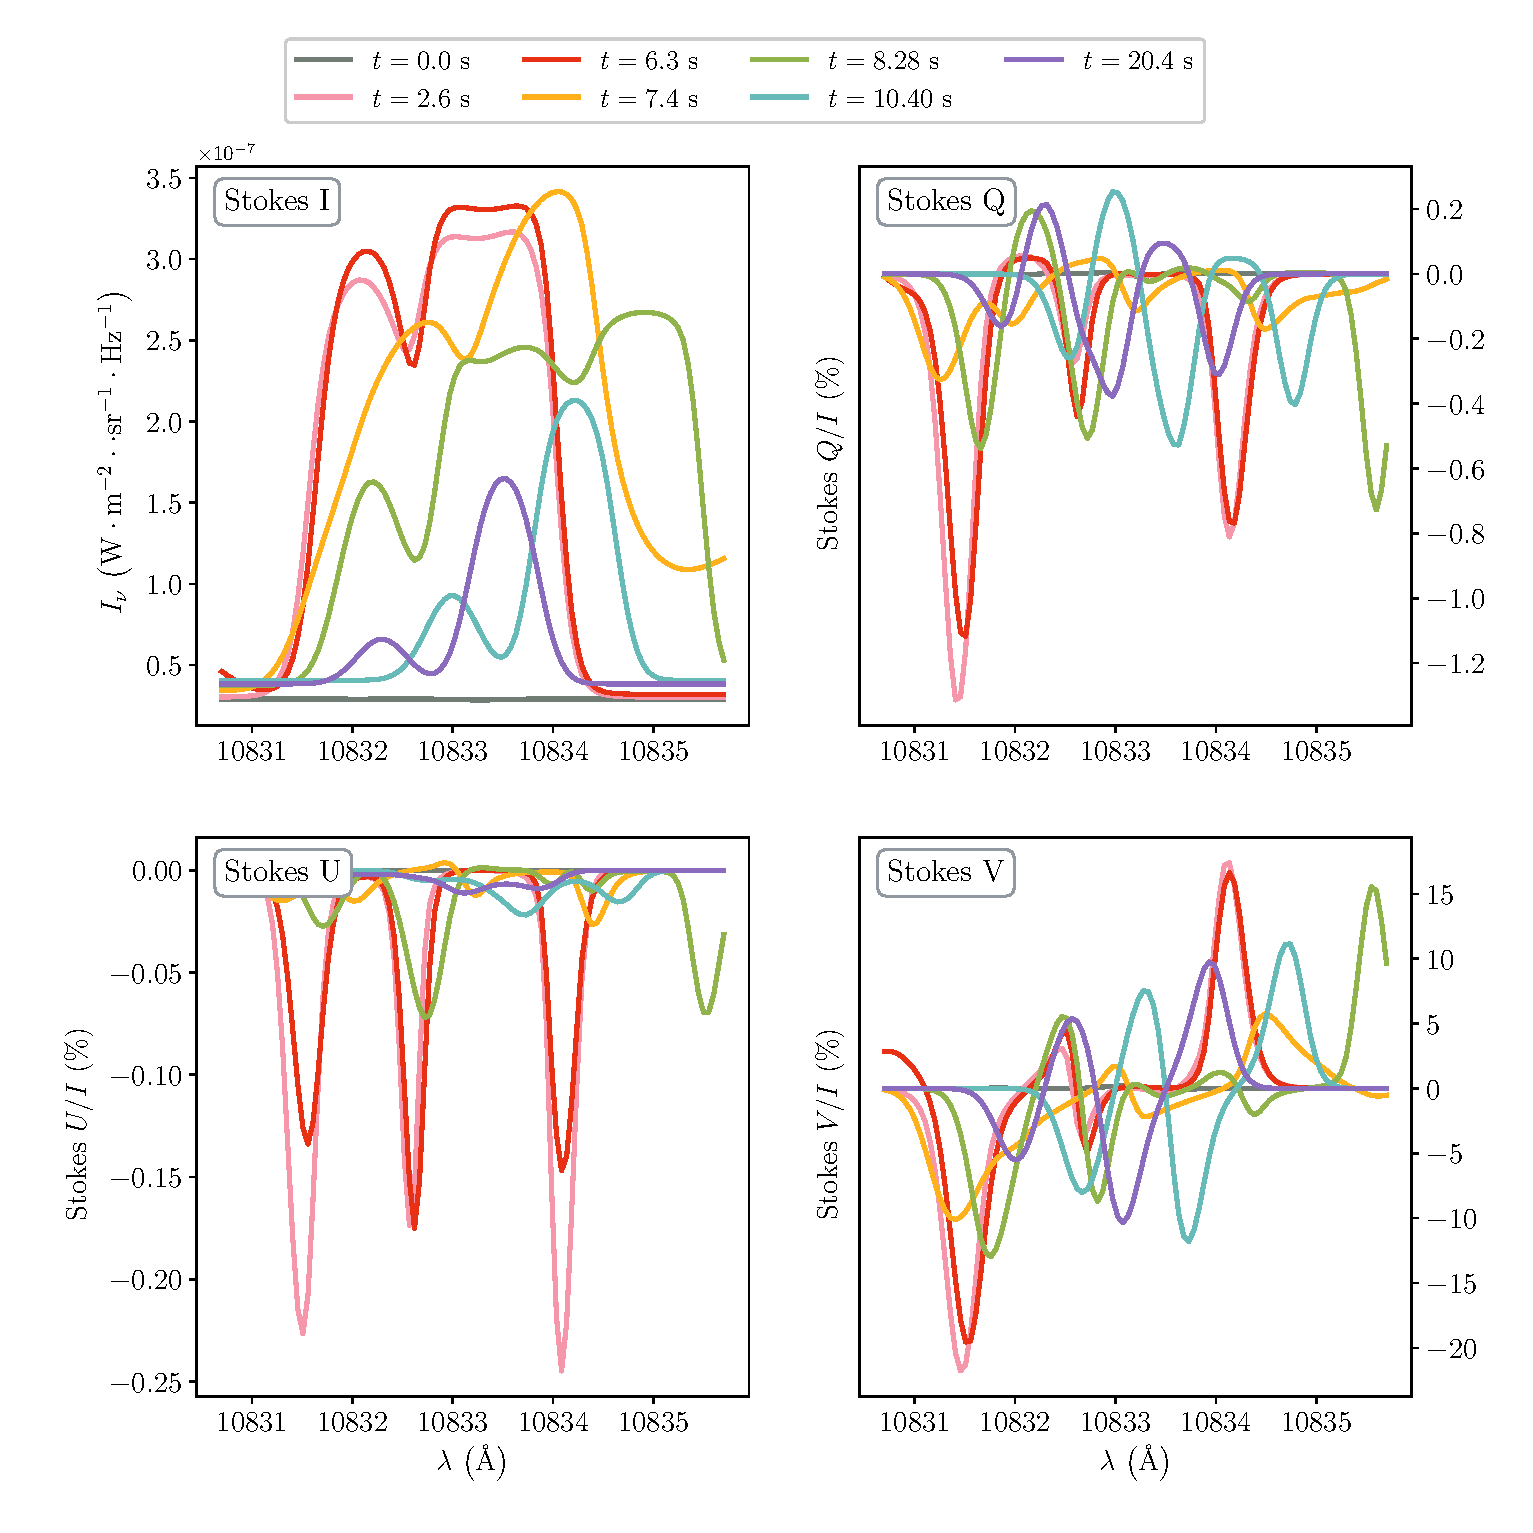
\includegraphics[width=0.6\textwidth]{figs/HeI_Stokes_spec}
	\caption{He \textsc{i} 10830 \mbox{\AA}线Stokes参数某些特定时刻的形状。}
	\label{fig:3.15}
\end{figure}
\section{讨论}\label{sec:3.8}
首先我们来关注如何解释Mg \textsc{ii}和C \textsc{ii}等谱线需要通过继续增大Stark宽度才能较好地再现耀斑带上谱线急剧致宽的谱线轮廓的问题。关于这一点,我们从目前RADYN和RH代码的一些缺陷出发,探讨模拟中可能忽略的一些重要效应:
\begin{enumerate}
	\item 非热电子的影响:显然入射的非热电子同样会对Mg \textsc{ii}的离子能级产生影响\parencites{Hawley2007},由于它们的能量往往更大,产生的Stark致宽效应也往往更强烈。尽管在我们的模型中这些入射的非热电子的密度$\sim10^{10}\ \mathrm{cm^{-3}}$往往远小于当地的热电子密度,但是它们应该仍然能够在热化的过程中和周围的其他电子相互作用,而这些局地的电子再与Mg \textsc{ii}离子能级产生相互作用。此外,这些非热电子对Mg \textsc{ii}粒子的非热激发和电离作用也会改变Mg \textsc{ii}离子的能级粒子数,从而影响谱线轮廓形状。以上和非热电子有关的因素都是目前的计算中所没有考虑的,我们的Stark致宽只考虑了周围热电子的影响,且没有考虑这些非热电子的非平衡电离效应。
	\item 三维辐射转移效应:\textcites{Leenaarts2013a}指出三维辐射转移效应对Mg \textsc{ii}谱线线心的形成至关重要。目前尚没有对耀斑过程中的色球谱线进行完全自洽大气内的三维辐射转移计算的工作,因此我们猜测其可能也会对谱线的致宽做出贡献。
	\item 磁场:模拟中没有考虑磁场对大气动力学演化的影响。尽管之前有相关研究表明Mg \textsc{ii}对磁场是有一定敏感性的\parencites{Ballester2016},但我们基于RH代码的计算表明,在1000 G左右的磁场并不能对辐射强度,即Stokes $I$参数产生重要的影响。
	\item 电子密度:\textcites{Rubio2017}通过手动增加大气中的电子密度至$\sim 10^{15}\ \mathrm{cm}^{-3}$来获得非线心反转的谱线,而这一电子密度的高峰已经在我们的自洽大气中找到。但是在她们的参数模拟中,这个电子密度的高峰在高度的分布上更广,甚至达到了线翼的形成位置。如果我们能够在自洽大气的线翼形成位置也能形成$10^{14}\ \mathrm{cm^{-3}}$以上的电子密度,是有可能进一步增大Stark致宽的。
\end{enumerate}

关于Mg \textsc{ii}谱线剧烈致宽的另外一个解释来自于\textcites{Rubio2017},她们认为多个尚未在观测上得以分辨的$200\ \mathrm{km\  s^{-1}}$以上的宏观物质对流叠加有能够产生剧烈致宽的谱线。在我们的模拟中,在$t=7.35$ s左右由于在一个一维大气中同时存在速度上流和下流,的确获得了剧烈加宽的Mg \textsc{ii} h和k线(见图~\ref{fig:3.4})。但是由于物质下流与致密的中低层色球大气的相互作用,此时刻附近的约为$100\ \mathrm{km \  s^{-1}}$的物质下流并不能在模拟上持续超过$1$ s的时间。因此不能产生超过1 \mbox{\AA}以上的远红翼的辐射增强。\textcites{Rubio2017}中假想存在的这样的高速度的物质下流(色球凝聚)可能来自于入射非热电子的能流不均匀导致的局部大于$10^{13}\ \mathrm{erg\  cm^2\  s^{-1}}$高能流\parencites{Kowalski2015,Kowalski2018a}。

\textcites{Panos2018}通过机器学习在一系列大耀斑的耀斑带前缘提取出了带有剧烈红翼增强和部分线心反转的Mg \textsc{ii} h和k谱线轮廓。在整个耀斑带前缘扫过这些区域后,出现的是常见的单峰、剧烈致宽的Mg \textsc{ii} h和k谱线轮廓。整个谱线的演化过程和我们5F11模型中的Mg \textsc{ii}演化过程比较类似。在我们的模拟过程中的$t=7-10$ s间先产生了有较大红移的Mg \textsc{ii} h和k线,而后这些谱线的红移逐渐减小,并且因为色球被高度压缩而产生的电子密度增加(至$\sim 8\times 10^{14}\ \mathrm{cm^{-3}}$)而出现了非线心反转的谱线。

最近\textcites{Tei2018}发现了Mg \textsc{ii}线在耀斑一开始发生时的蓝移(蓝翼增强)现象。在此之后,Mg \textsc{ii}谱线才出现常见的红翼不对称性。她们认为这个蓝翼的增强来自于一个上流的冷物质湍,并用一个简单的云模型计算了Mg \textsc{ii}谱线的辐射转移。她们发现对于当这团物质温度为$T=10^4$ K且上流速度为$v_z\sim 40\ \mathrm{km \  s^{-1}}$时能够非常好的拟合观测到的谱线。正如图~\ref{fig:3.13}右栏所示的,我们的5F11模拟中也同样发现具有蓝翼增强的谱线情况,且出现在整个谱线轮廓的剧烈红移发生之前。在我们的模拟中这团冷物质的温度大约为$4\times 10^4$ K,速度约为$\sim 36\ \mathrm{km \  s^{-1}}$。由于在模拟中的这团物质温度较高,因此在C \textsc{ii}和Si \textsc{iv}线上也能看到蓝翼增强的分量,这与她们的观测有一定的差异。同时我们的这团冷物质的存在时间只有$\sim 1-2$ s,而\textcites{Tei2018}则发现了整个谱线蓝移过程持续了数十秒。尽管如此,我们的模拟还是支持她们对Mg \textsc{ii}谱线在耀斑带开始增亮时出现蓝翼增强的解释。

\begin{figure}
	\centering
	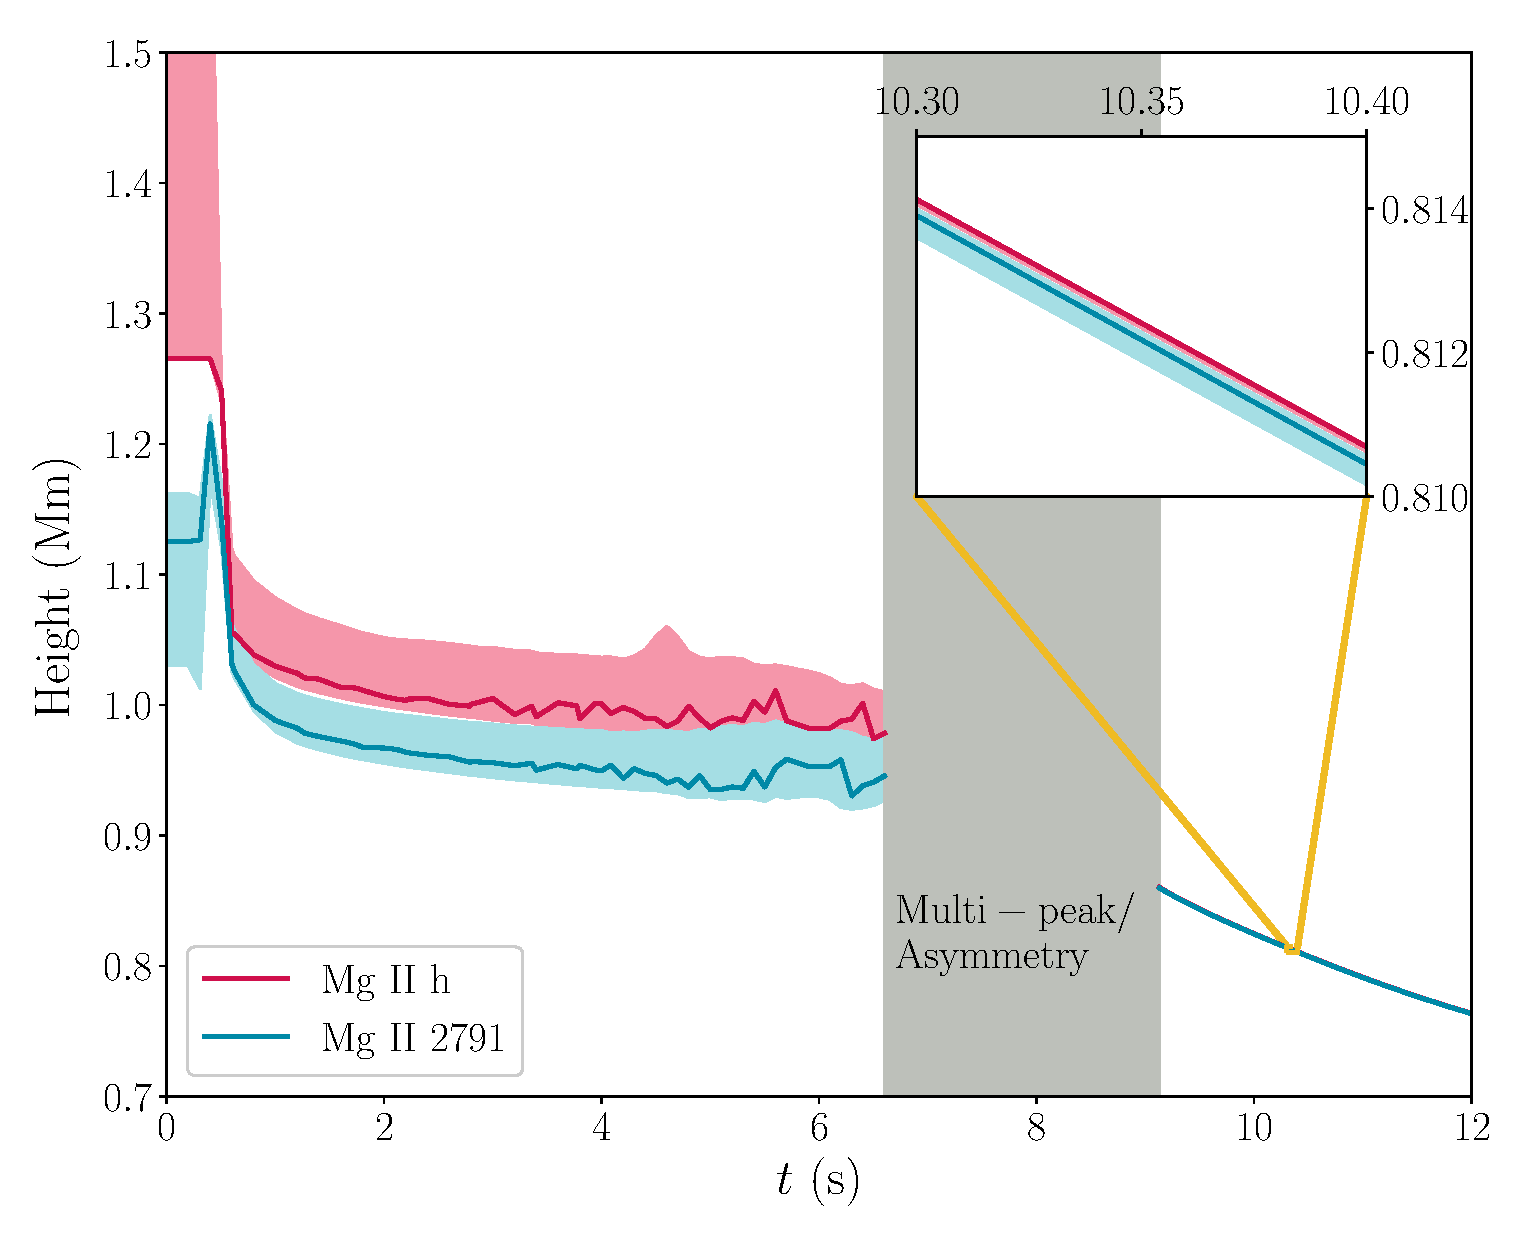
\includegraphics[width=0.6\textwidth]{figs/formation_height}
	\caption{5F11模型中Mg \textsc{ii} k与2791三重线线心形成位置随着时间的演化图。我们通过积累贡献函数$C_I'=0.16$与$C_I'=0.84$来确定整个谱线的形成区间。其中青色代表Mg \textsc{ii} 2791 \mbox{\AA}线,红色代表Mg \textsc{ii} k线。灰色部分代表由于谱线的过于不对称和多峰结构导致无法确定线心位置的时刻。}
	\label{fig:3.16}
\end{figure}
另外值得一提的是我们发现在模拟后期Mg \textsc{ii} h和k线出现非线心反转谱线轮廓时,Mg \textsc{ii}三重线往往形成在同一大气高度上。之前对于宁静太阳上Mg \textsc{ii}线心的形成模拟认为它们形成在大约在过渡区下200 km\parencites{Leenaarts2013b}的高度。而Mg \textsc{ii}三重线则一般被认为形成在低色球位置\parencites{Pereira2015}。但一些在耀斑带上的一维辐射流体力学模拟表明也可以形成在较高的色球位置,约为0.83 Mm - 1.14 Mm\parencites{Rubio2017}。为了确认这一点,我们画出了Mg \textsc{ii} k线和2791三重线的形成高度随着时间的演化图(图~\ref{fig:3.16})。我们发现,一开始的大气中Mg \textsc{ii} k线心的确形成于高色球,而2791三重线线心则形成在低色球。随着时间的不断演化,$t=4$ s时两条谱线的形成区域已经相当接近且出现重叠,而当$t>10$ s后两条谱线的线心形成位置几乎是完全相同的,同样的结果同样被其他的一维辐射流体力学模拟所证实\parencites{Kerr2019}。因此我们认为当Mg \textsc{ii} h和k线出现非线心反转的谱线时,处于发射状态的Mg \textsc{ii}三重线线心很有可能形成于高色球,只能作为低色球加热的定性判据,而不应该作为定量诊断工具。

对于为什么C \textsc{ii}线和Si \textsc{iv}线难以在Mg \textsc{ii}线和观测拟合比较好的时间点再现观测到的谱线轮廓,我们也可以从目前的模拟给出一定的猜测。总的来说,我们认为目前一维辐射流体力学模拟较为欠缺的一个点是对耀斑衰变相中冷却过程的模拟。目前对这些这样的较长时间红翼不对称性的产生机制基本都集中在冷却过程上,如\textcites{Tian2015}和~\textcites{Brannon2016}认为产生需要冷却物质的下流,\textcites{Reep2016}和~\textcites{Warren2016}认为需要多个耀斑环的持续冷却。在我们的模拟中,整个色球凝聚过程随着电子束入射能流的减小而迅速减弱,不能一直产生较长时间的物质下流。因此如何在模拟上再现这样持续时间非常长的色球凝聚过程仍是亟待解决的问题。另外在我们的模拟中,C \textsc{ii}谱线的线心形成高度和Mg \textsc{ii}非常相近,但是线翼却相对高于Mg \textsc{ii}线,在实际情况中是否可能在这段区间内存在较大的速度梯度进而有足够的速度流产生大量的红翼辐射仍然存疑。

对于Si \textsc{iv}线,在之前\ref{sec:3.7}节的贡献函数分析中我们提到在模拟的合成光谱中存在来自色球温度较低的贡献。现在我们认为这些贡献实际上是来自于我们在RH代码中使用的原子模型未包含Si \textsc{i}和Si \textsc{ii}能级造成的错误。在Mg \textsc{ii}线的模拟中,我们之所以能够使用一个不包含Mg \textsc{i}原子模型的Mg \textsc{ii}离子模型去模拟谱线形成,其原因是Mg \textsc{i}和Mg \textsc{ii}都广泛存在于整个光球和中低色球的大气中,因此我们并不需要非常仔细地去考虑其电离态上的粒子数对Mg \textsc{ii}线心附近轮廓的影响。

而对于Si则恰恰相反,Si \textsc{iii}之下还有两个低电离态Si \textsc{i}和Si \textsc{ii},在低层大气中这几个电离态之间的相对粒子数对温度是相对敏感的(见图~\ref{fig:3.16})。因此如果我们在原子能级中不考虑这两个电离态,一个直接的结果是在低层大气中,本来应该大量处在Si \textsc{i}和Si \textsc{ii}能级上的原子被我们强行留在了Si \textsc{iii}和Si \textsc{iv}能级上,特别是在耀斑过程中,由于色球凝聚的出现,中低色球的密度大大增加,导致了有更多应该在Si \textsc{i}和Si \textsc{ii}能级上的原子被滞留在高能级上,产生了不应该存在Si \textsc{iv}谱线辐射。因此我们强调如果要比较好的模拟Si \textsc{iv}在太阳爆发过程中的谱线轮廓,应该使用包含Si \textsc{i}和Si \textsc{ii}两个能级的原子模型。
\begin{figure}
	\centering
	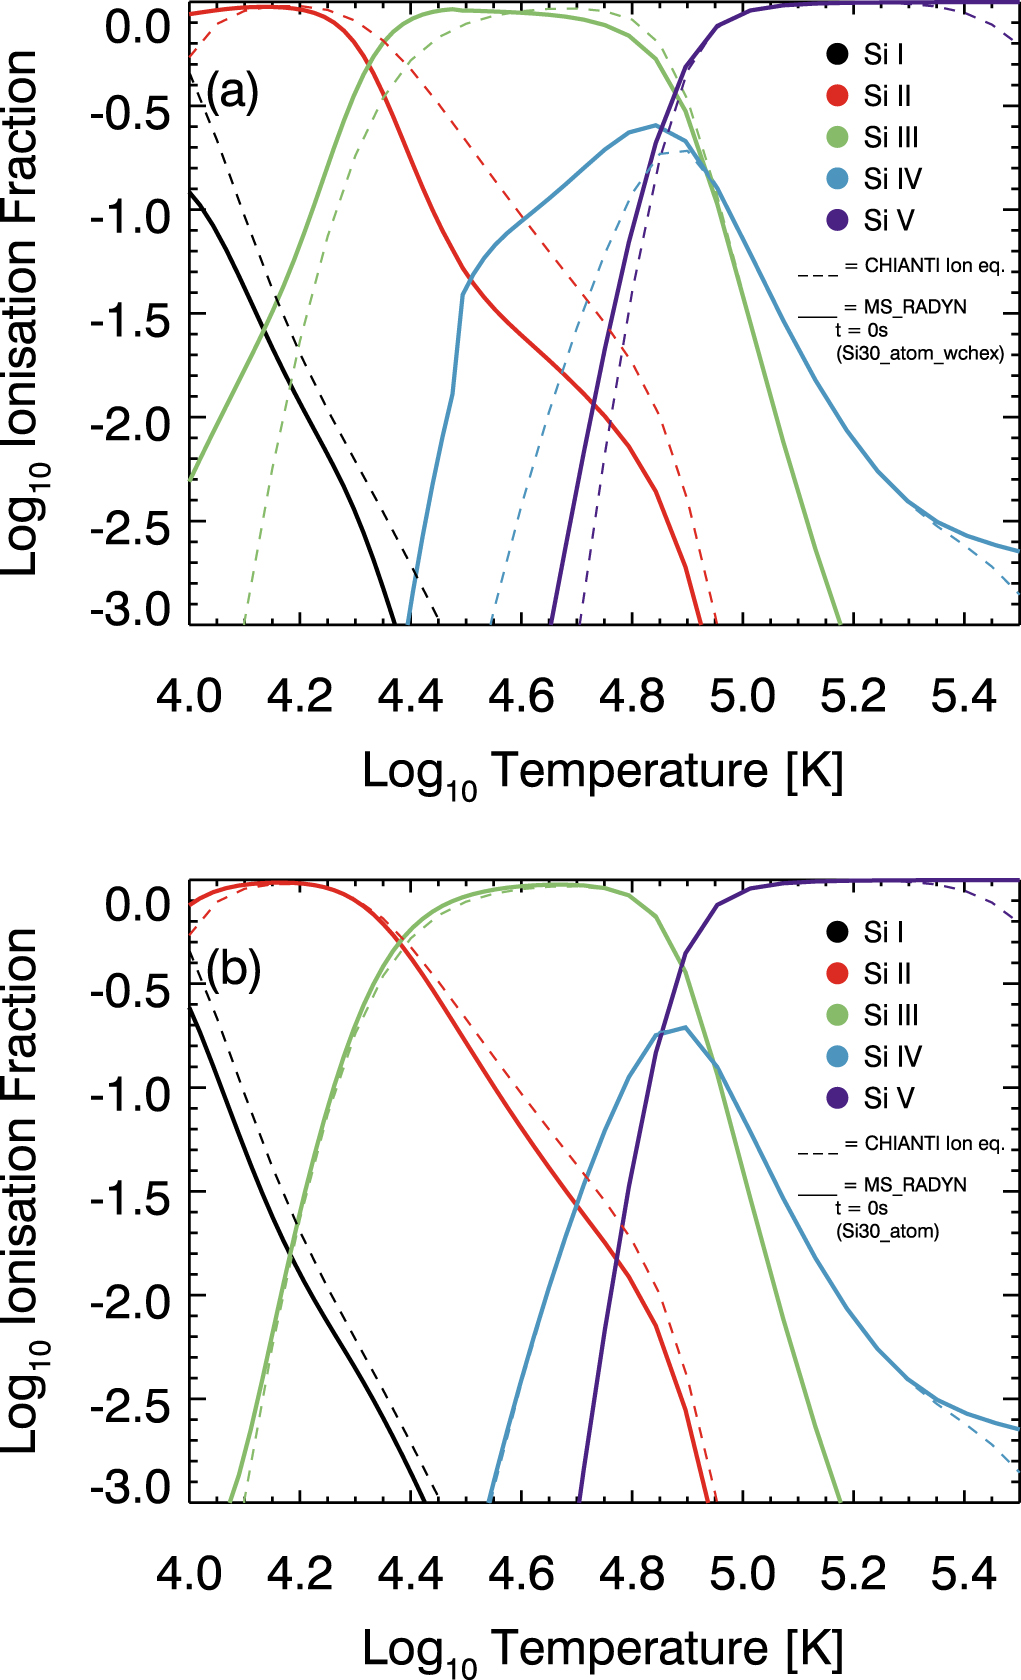
\includegraphics[width=0.5\textwidth]{figs/Si_pop}
	\caption{Si原子在不考虑电荷交换(上)和考虑电荷交换(下)的不同电离态占据数与温度之间的关系。来源:\textcites{Kerr2019}}
	\label{fig:3.16}
\end{figure}


% vim:ts=4:sw=4
	% Copyright (c) 2014,2016 Casper Ti. Vector
% Public domain.

\chapter{参数研究:Mg \textsc{ii}谱线在M矮星耀斑非热电子束加热下的响应}\label{chap:4}
在这一章节中我们将通过一系列不同入射非热电子参数的一维辐射流体力学模拟,在一个较为简单的参数空间内寻找在M矮星耀斑中可能出现的Mg \textsc{ii}线谱线轮廓。由于目前我们对M矮星耀斑的紫外光谱观测并不多,尤其是获取高分辨率的紫外谱线观测更加困难\parencites{Hawley2007,Kowalski2019,Froning2019},因此我们选择了一个相对较大的参数空间来进行模拟。我们希望通过整个大的参数空间的搜索,勾勒出不同非热电子束参数下M矮星耀斑带上的Mg \textsc{ii}谱线辐射轮廓特征。

另外需要注意的一点是,由于是对恒星的观测,我们的直接观测量不再是辐射强度$I_\nu$而是辐射流量$F_\nu$,同时由于整个恒星存在着背景光谱,因此有必要减去耀斑发生前的初始SED,得到耀斑带上的净辐射流量。
\section{初始条件设定}
我们同样利用RADYN代码来计算非热电子束入射大气之后整个低层大气的动力学演化过程。初始大气采用了RADYN代码中的M矮星初始大气,环长10 Mm(参见~\ref{sec:2.1.4})。整个电子束参数空间中,我们都取谱指数$\delta = 3$,变化的是电子束能流和截止能量$E_c$。我们考虑了三种不同的能流模型,1F11,1F12和1F13,每种能流模型都计算了截止能量在$E_c = 85,\ 150,\ 200,\ 350$和$500$ KeV的结果,故一共有15种不同电子束参数的模型输出。整个电子束的能流变化采用了一个爆发(\textit{burst})型的轮廓\parencites{Aschwanden2004a,Aschwanden2004b},其半高全宽为2 s。

我们选取这些和太阳耀斑有较大区别的非热电子束参数作为我们整个参数研究的输入的主要原因是为了产生能够和具体观测上相拟合的$T\sim 10000$ K 的白光连续谱。这些高能流、高截止能量$E_c$的非热电子束能够穿透恒星色球大气,直接加热色球底层甚至光球部分。通过加热这些密度较高的低层大气来产生明显的连续谱辐射。这些RADYN输出文件已经被Adam F. Kowalski等人用于研究如何在模拟上再现M矮星耀斑$T\sim 10000$ K的白光黑体谱,Balmer跳跃比,H$\gamma$和4170 \mbox{\AA}连续谱强度比等一系列参数特征。最终他们发现,能流为1F13,截止能量$E_c = 85$ KeV,谱指数$\delta = 3$的模型能够同时较好地再现观测到的持续性的白光连续谱、Balmer线系谱线致宽与低层大气加热等一系列特征。在此基础上,我们将这些RADYN大气输出转化为RH+SB代码的输入文件,计算Mg \textsc{ii}谱线随着模拟时间的演化,并对其形成高度的变化做一定分析。
\section{大气演化特征}\label{sec:4.2}
我们在图~\ref{fig:4.1},\ref{fig:4.2}和\ref{fig:4.3}中分别展示了1F11,1F12和1F13模型中温度$T$,电子密度$n_e$和一维速度$v_z$在$t=1,\ 2,\ 3,\ 5$和8 s时刻在不同高度上的分布。可以很明显的看到,不同的电子束参数对整个大气的动力学演化过程起了相当不同的作用。

对于1F11模型来说,整个底色球大气一般从$\sim 5\times 10^3$ K被加热到$\sim 7\times 10^3$ K,并在0.1-0.4 Mm间形成一个温度的平台。在0.4 Mm以下,电子密度$n_e$随着这部分大气的加热而迅速上升$1-3$个量级,最高能够达到约$\sim 10^{14}\ \mathrm{cm^{-3}}$。对低层大气的加热同样激发了物质流动。与太阳大气不同的是,在宏观速度上模拟中主要出现的是色球蒸发现象,即向上的宏观物质流动,而并没有太多向下的物质流动,且并没有明显的色球层被压缩的特征,可能是因为电子束加热位置高度比较低,密度已经比较大的原因。

不同截止能量$E_c$也对整个大气参数的变化产生了不同的影响,简单的来说,$E_c$越大,加热的位置越低,且局地密度越大。在温度上,$E_c$较大时还能在大约$\sim 0.15$ Mm的高度上形成一个局部的温度极值。电子密度$n_e$的变化趋势类似,$E_c$越大,电子密度极值出现的高度越低。对于一维速度$v_z$,较小的$E_c$(85, 150 KeV)尚能在星冕中产生一定的速度上流$\sim 10\ \mathrm{km \  s^{-1}}$,但当$E_c$较大时,物质上流基本都局限在色球内,且速度只有$\sim 5\ \mathrm{km \  s^{-1}}$。

\begin{figure}
	\centering
	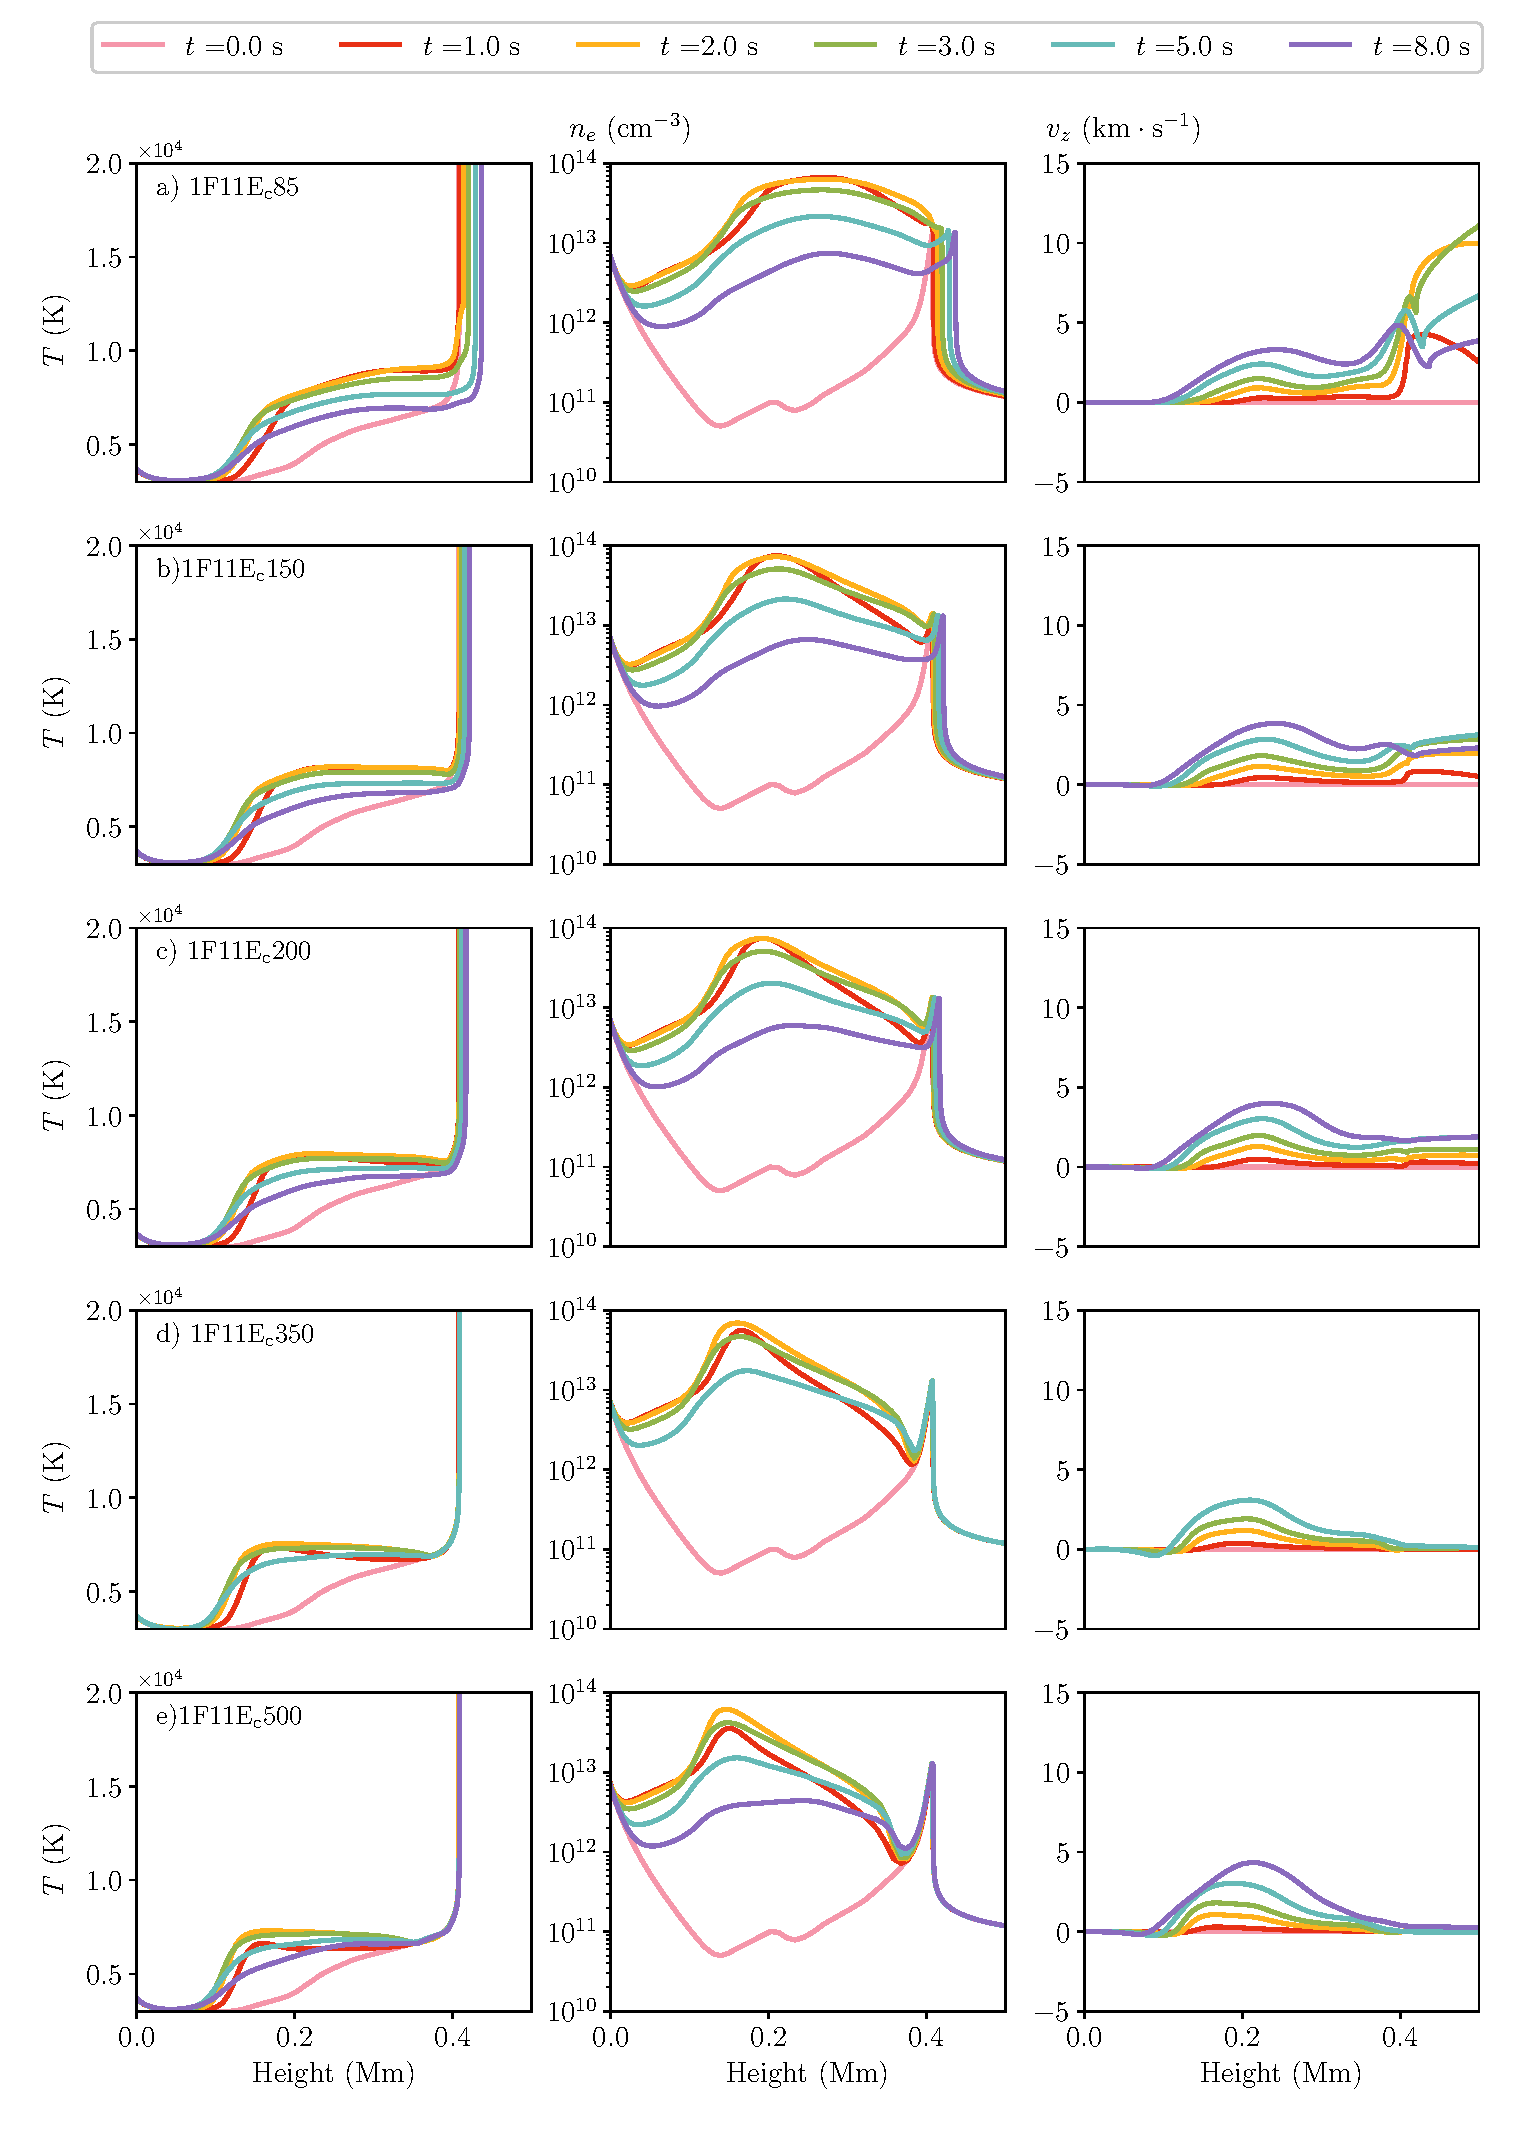
\includegraphics[width=\textwidth]{figs/dMe_atoms_1}
	\caption{各1F11模型中一些特征时刻温度$T$,电子密度$n_e$,一维速度$v_z$随高度分布图。}
	\label{fig:4.1}
\end{figure}

对1F12模型而言,更大的能流输入能够产生更加动态的低层大气。总的来说相比于1F11模型,低层大气能够被加热到更高的温度$\sim 9\times 10^{3}$ K,且能够产生更高的电子密度,接近$10^{15}\ \mathrm{cm^{-3}}$。在$E_c = 85,\ 150 ,\ 200$ KeV时还能在星冕中形成较为可观的物质上流,并且推动过渡区位置上移。

对于高截止能量$E_c$的情况,更低位置的加热使其倾向于产生更低位置的温度极值,且高色球和过渡区基本没有明显的温度、电子密度变化。而对低截止能量$E_c$,仍有部分能量被释放在高色球,使得高色球的温度和电子密度有较大程度的上升,其中温度甚至能够一度上升$10^4$ K达到$2\times 10^4$ K。

\begin{figure}
	\centering
	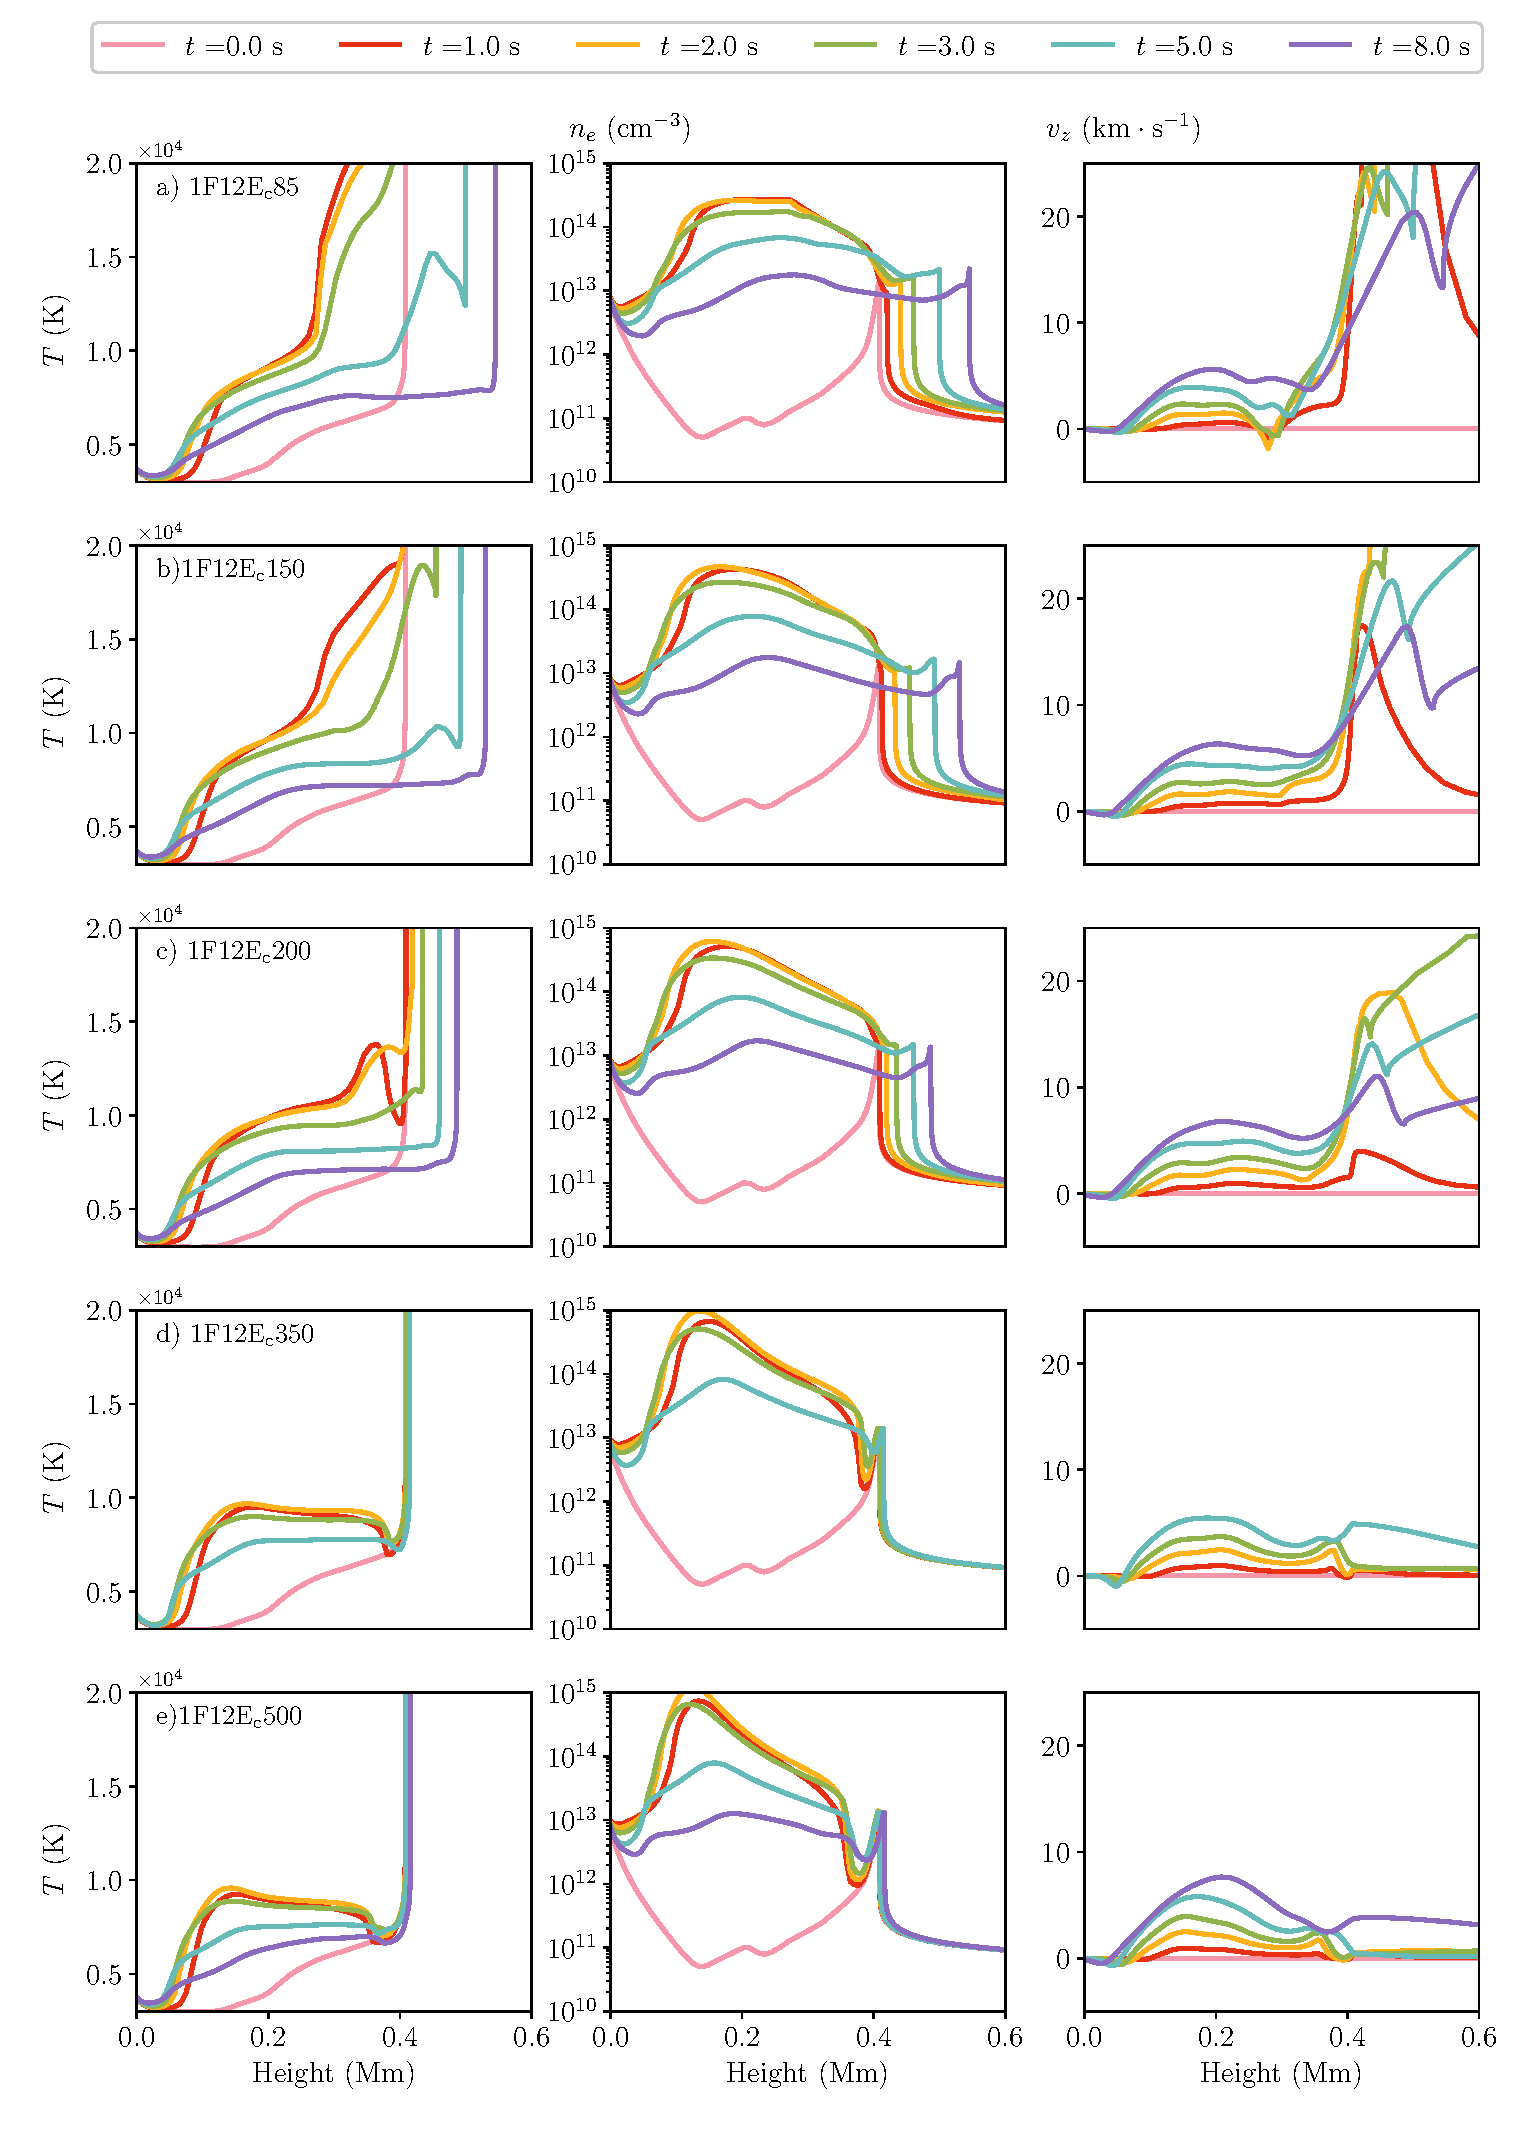
\includegraphics[width=\textwidth]{figs/dMe_atoms_2}
	\caption{各1F12模型中一些特征时刻温度$T$,电子密度$n_e$,一维速度$v_z$随高度分布图。}
	\label{fig:4.2}
\end{figure}

1F13模型相比之前的1F11和1F12模型注入了更大的能流,因此即使是高截止能量下,高色球仍有相当一部分被从低于$10^4$ K的温度加热到$2\times10^4$ K以上。整个中低色球在爆发相的平均温度大约为$\sim 1.5\times 10^4$ K。电子密度$n_e$在爆发相中最高能够达到$10^{16}\ \mathrm{cm^{-3}}$。色球蒸发在色球区域的特征速度大约为$\sim 10-20\ \mathrm{km \  s^{-1}}$。同样高截止能量$E_c$伴随着更低大气中的温度上升,在500 KeV中甚至能在0.1 Mm上达到$2\times 10^4$ K。除了$E_c = 85$ KeV的情况,其他大气中的过渡区伴随着色球蒸发有相对上升。在$E_c = 85$ KeV时色球蒸发的速度上流主要在过渡区以上。

\begin{figure}
	\centering
	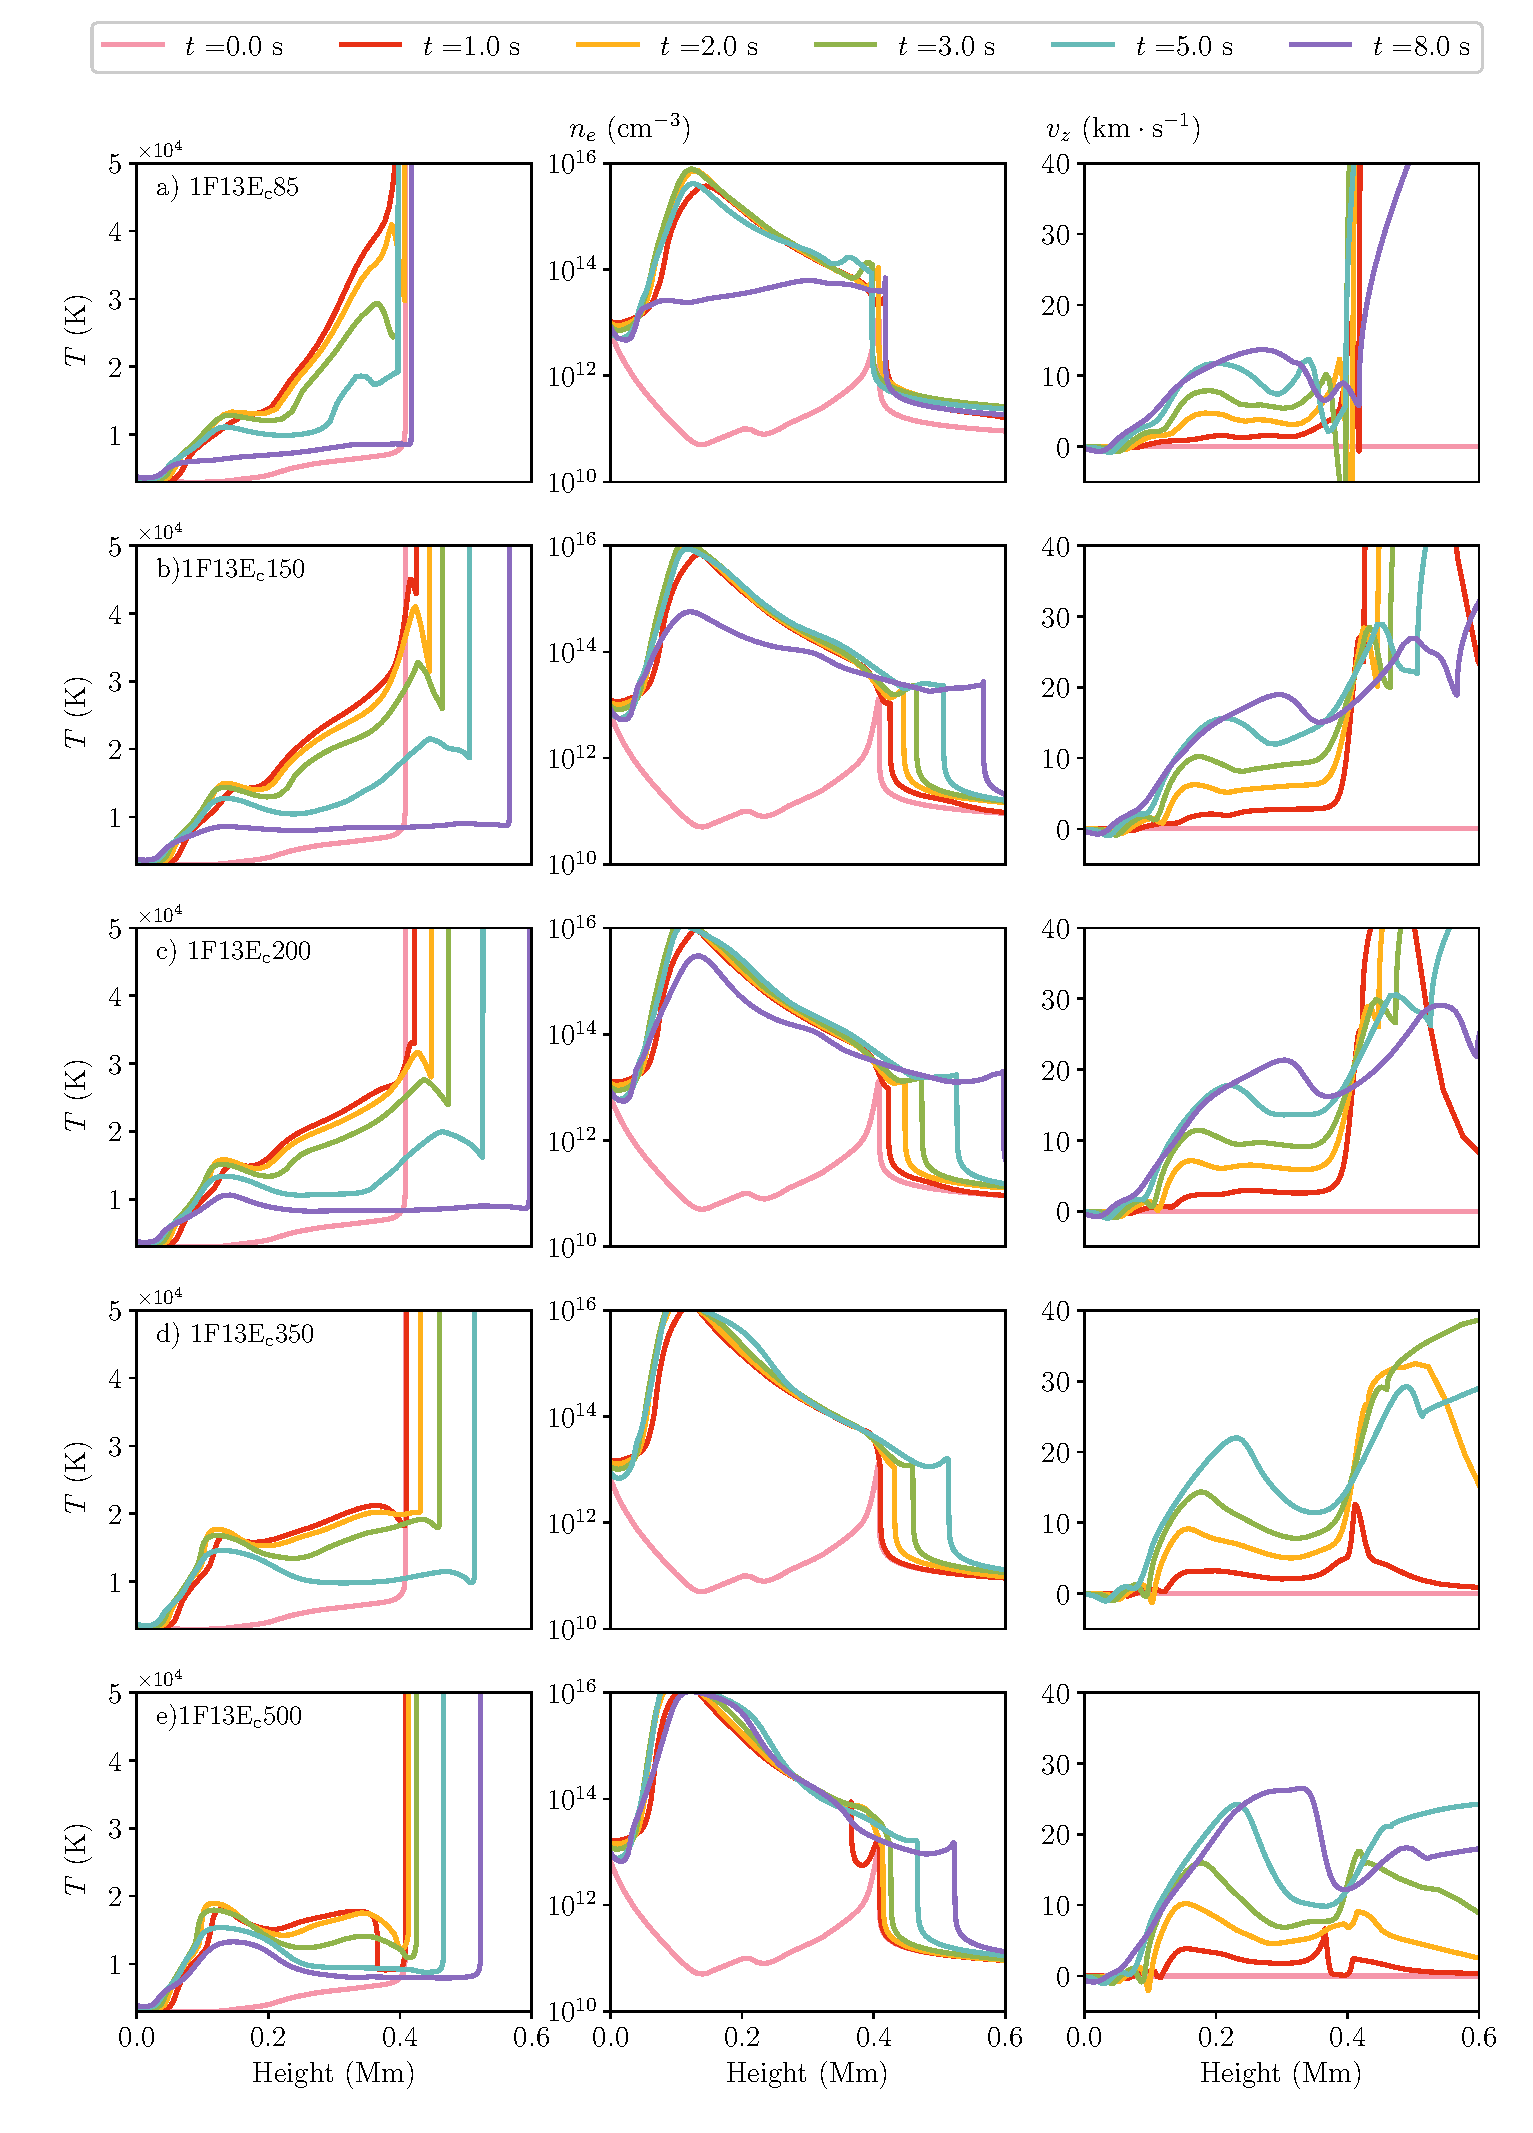
\includegraphics[width=\textwidth]{figs/dMe_atoms_3}
	\caption{各1F13模型中一些特征时刻温度$T$,电子密度$n_e$,一维速度$v_z$随高度分布图。}
	\label{fig:4.3}
\end{figure}

\section{谱线演化特征}\label{sec:4.3}
在这一部分我们将讨论各个模型中的Mg \textsc{ii}谱线演化过程。由于不同非热电子加热大气不同,Mg \textsc{ii}谱线对其也会产生不同的响应。图~\ref{fig:4.4}展示了各个模型中的所有时刻的Mg \textsc{ii} h谱线内总辐射流量随着时间的演化。图~\ref{fig:4.5}展示了~\ref{sec:4.2}节中研究的各个特征时刻的Mg \textsc{ii} h净辐射流量(已经减去初始宁静大气的辐射流量)。可以看到由于整个谱线轮廓较广的形成范围,Mg \textsc{ii} h谱线轮廓事实上包含了两个重要的组成部分,一是线心部分形成于高色球的辐射,和来自于低色球的线翼辐射。因此整个Mg \textsc{ii} h线轮廓形状同时和高低色球两部分的大气参数有着密切联系。

在1F11模型中,除了$E_c=85$ KeV的情况,其他较高截止能量的情况下高色球大气几乎没有变化,因此线心部分的谱线轮廓几乎不发生变化。但是由于低层大气的加热,周围连续谱会有比较强的增强,主要来自于Balmer连续谱的贡献。此外,在部分截止能量$E_c$并不是太大的模拟中,电子密度的高峰并不位于非常深的大气中,而是接近于Mg \textsc{ii} h线翼和线心的形成位置,此时Stark致宽在远线翼位置会发挥比较重要的作用,非常强烈地增强了远线翼的辐射(如图~\ref{fig:4.4}和图~\ref{fig:4.5}的a, b, c等栏)。而此时线心位置如果没有足够的辐射增强(只有$E_c=85$ KeV时比较明显),整个净谱线轮廓会从发射变为吸收(但是真正的谱线轮廓还是发射线)。

在1F12模型中,由于能流有了相对增强,在$E_c=85,\ 150$和200 KeV模拟中基本都可以看到Mg \textsc{ii} h线心辐射的增强。且原来线心反转的谱线出现明显的红翼增强,在某些时刻甚至出现了非线心反转的谱线轮廓($t=2.0$ s等)。而在$E_c$较大时的谱线轮廓和1F11类似,都是连续谱剧烈增强但线心辐射基本没有明显变化,净谱线轮廓看上去像是吸收线。

1F13模型的谱线轮廓和之前的两个模型有较大不同,其一是由于低色球和高光球都被加热,因此整个谱线线翼的连续谱都剧烈增强。而且这些增强并非全部来自于Mg \textsc{ii} h线自身的Stark致宽,还有大量由于自由电子复合过程产生的Balmer连续谱的贡献。由于在高色球Mg \textsc{ii}线线心形成位置形成了较大的速度上流,谱线普遍表现出一定的蓝移特征,且伴随着一定的红翼辐射增强。在$E_c = 350$和500 KeV的模拟中,由于连续谱过于剧烈的增强,再发射也无法抵消吸收,Mg \textsc{ii} h线真的成为了吸收线。由于谱线的不对称性,在部分$E_c = 350$ KeV的谱线中可以看到红翼出现发射,而蓝翼出现吸收的特殊净谱线轮廓。


\begin{figure}
	\centering
	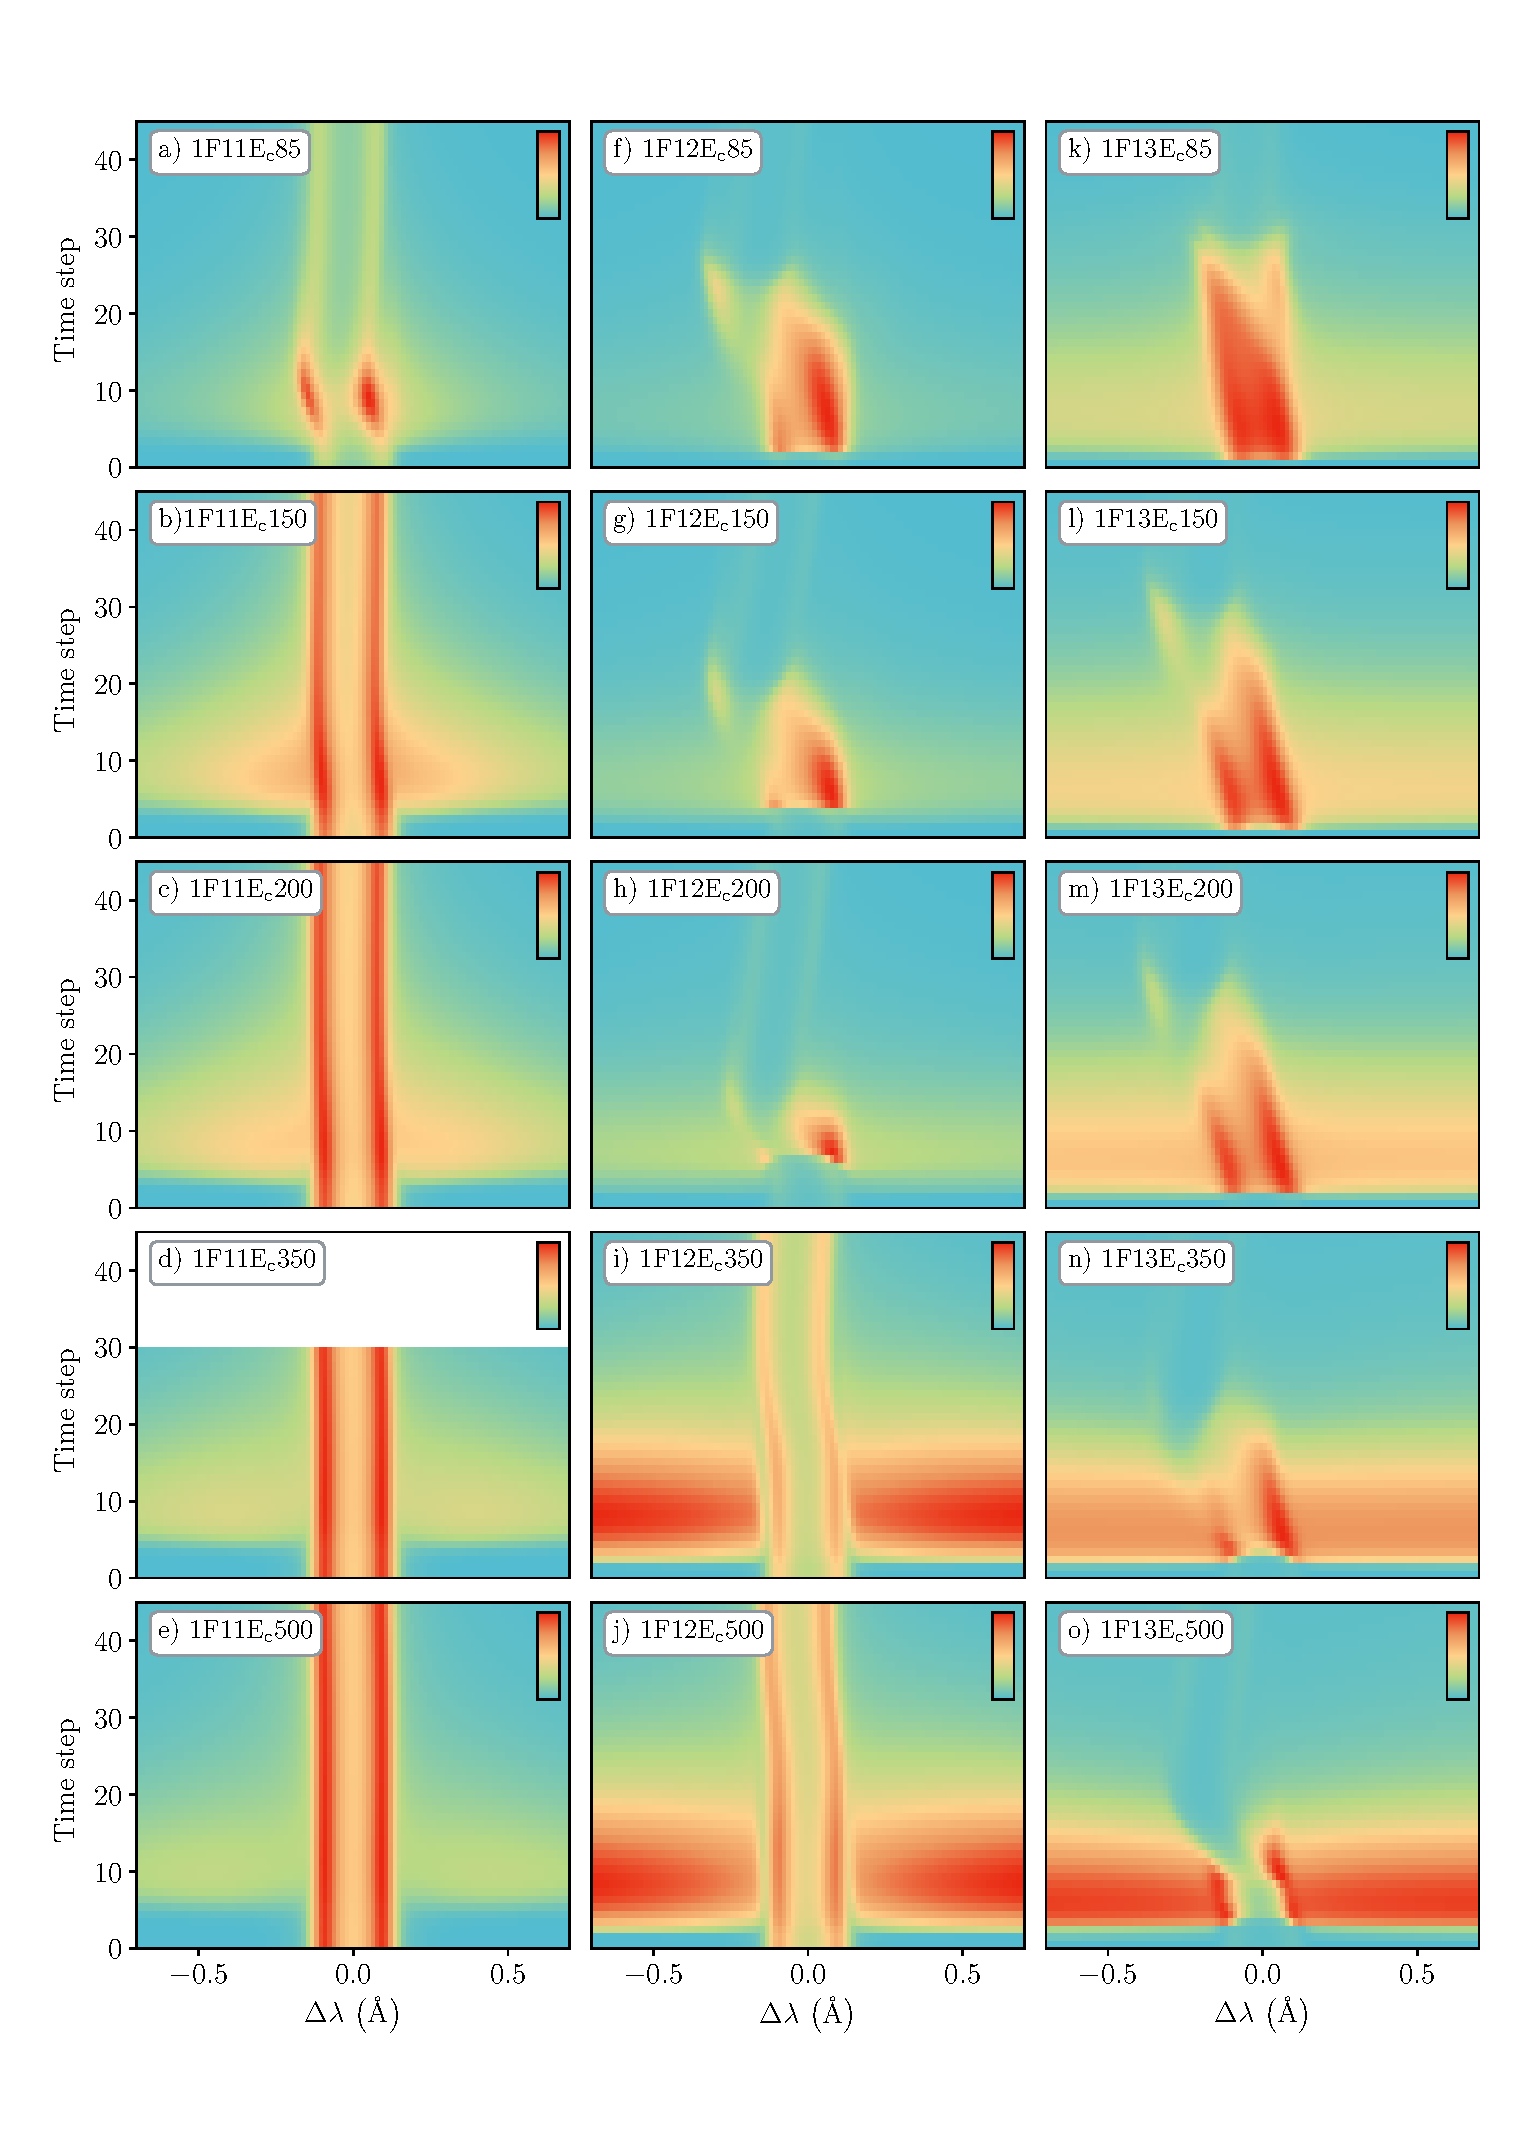
\includegraphics[width=\textwidth]{figs/dMe_MgIIh}
	\caption{Mg \textsc{ii} h线在不同电子束参数的模拟中的谱线流量随时间演化图。横坐标为波长,纵坐标为不同时刻,颜色代表该波长和时刻下的辐射流量。}
	\label{fig:4.4}
\end{figure}

\begin{figure}
	\centering
	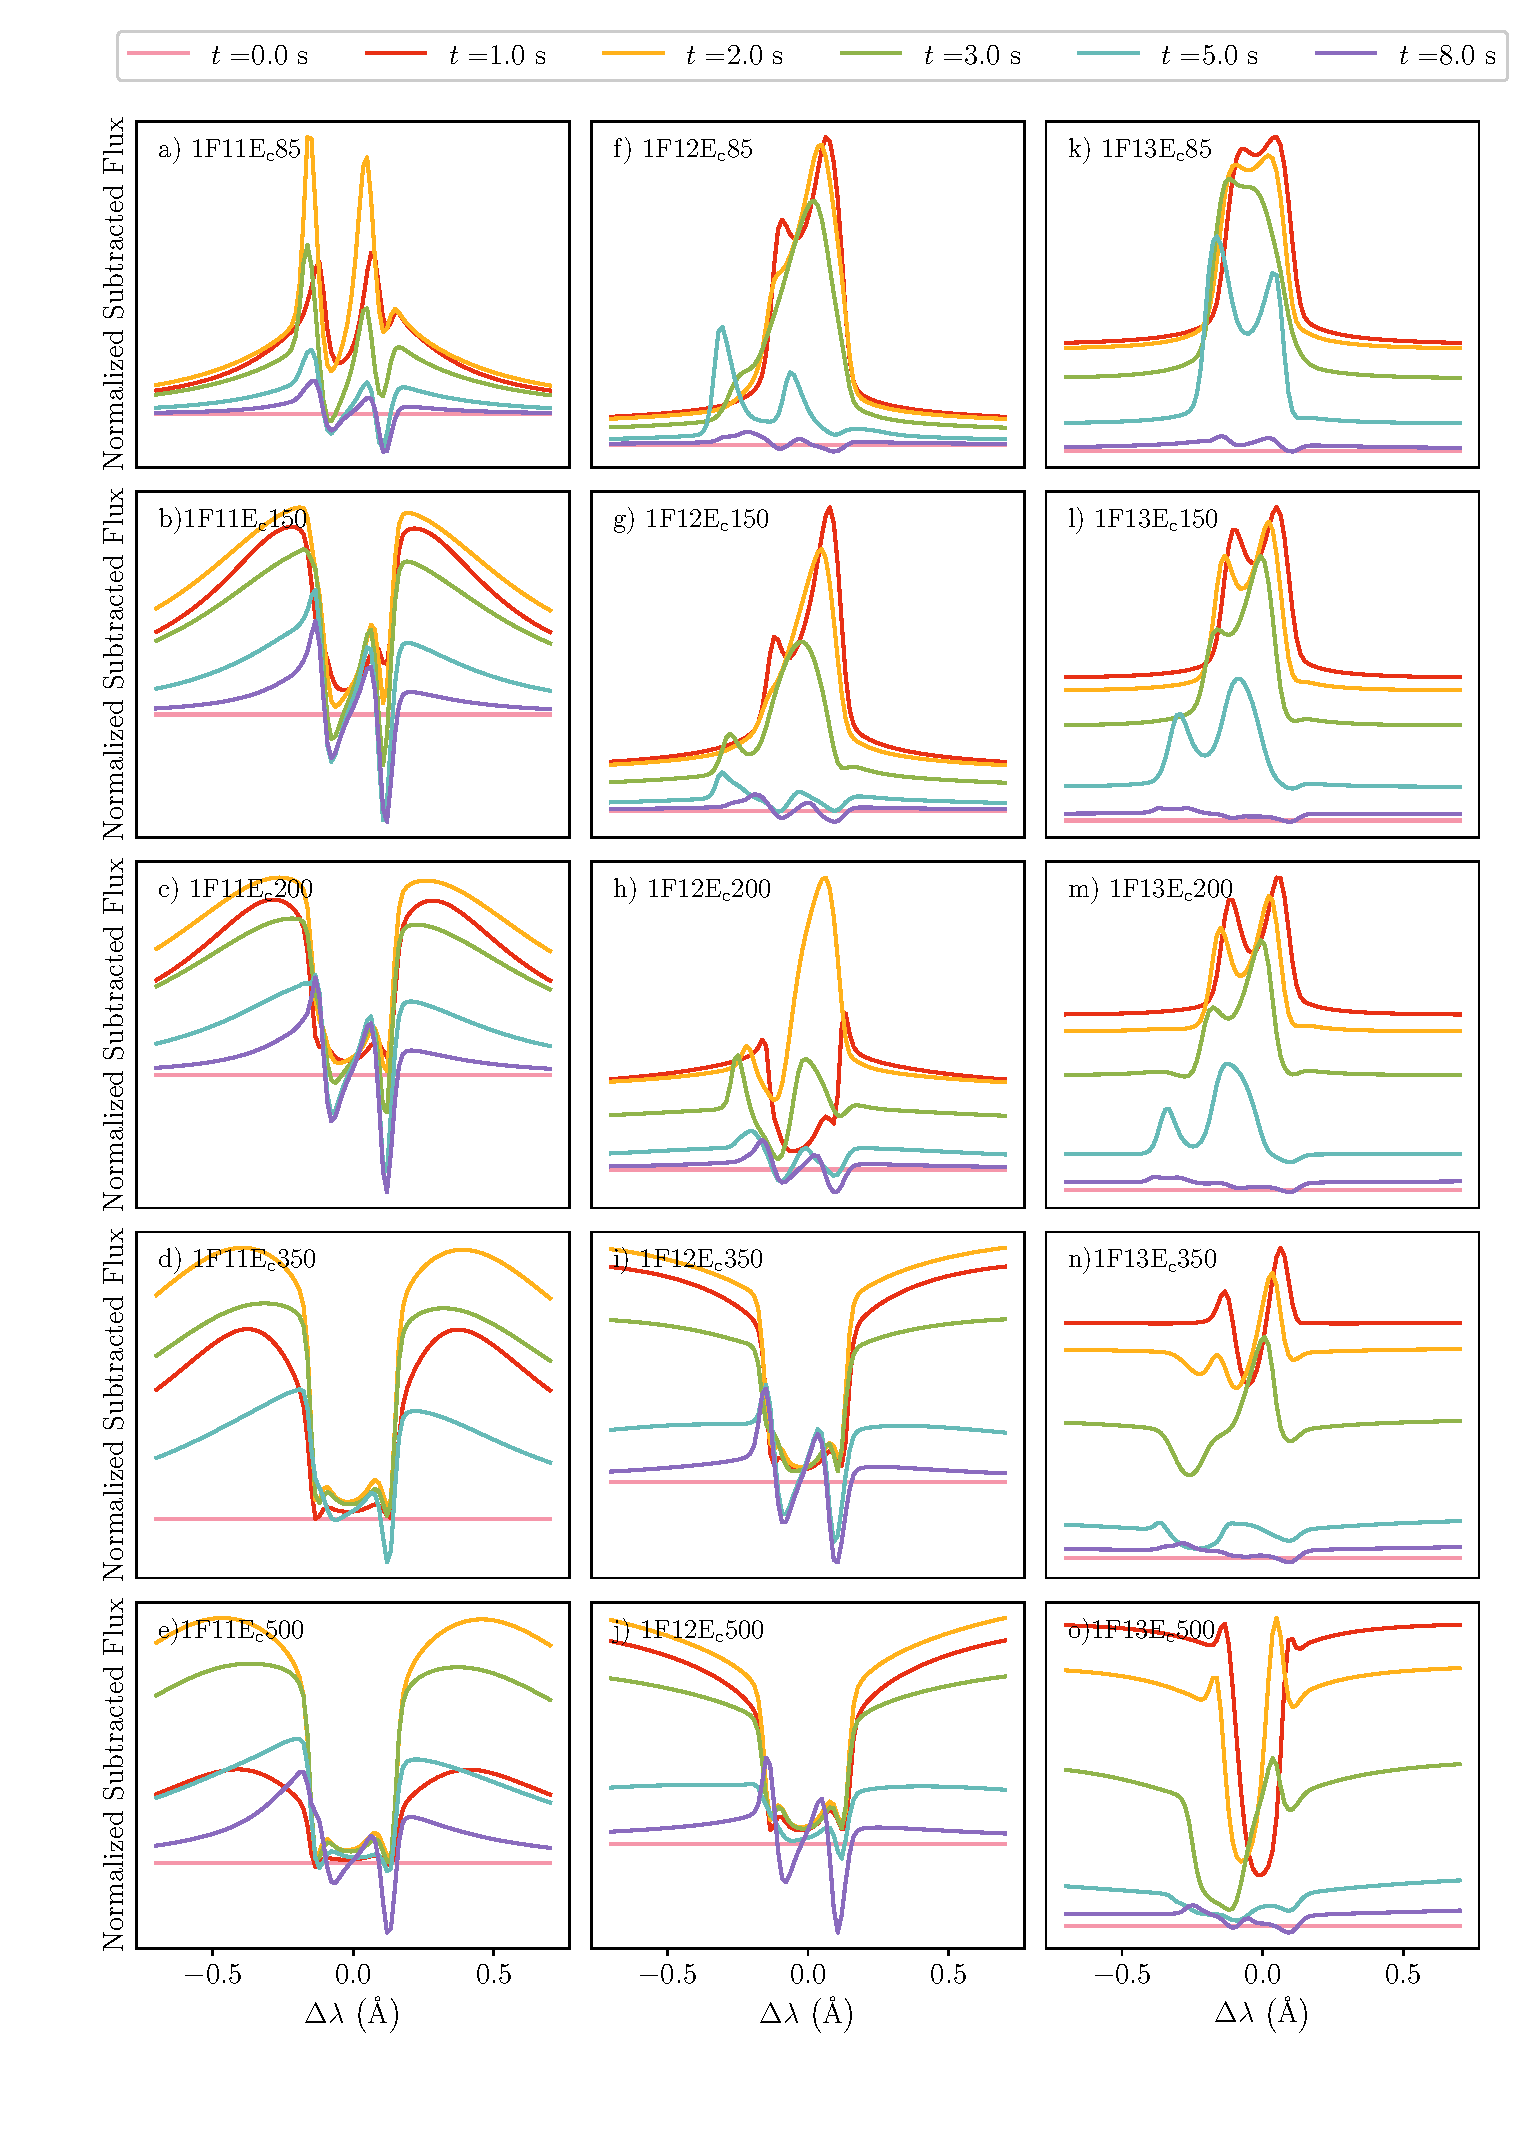
\includegraphics[width=\textwidth]{figs/dMe_MgIIh_spec}
	\caption{Mg \textsc{ii} h线在不同电子束参数的模拟一些特征时刻的谱线轮廓。注意图中展示的是已经减掉宁静初始大气辐射的净辐射流量。}
	\label{fig:4.5}
\end{figure}

\begin{figure}
	\centering
	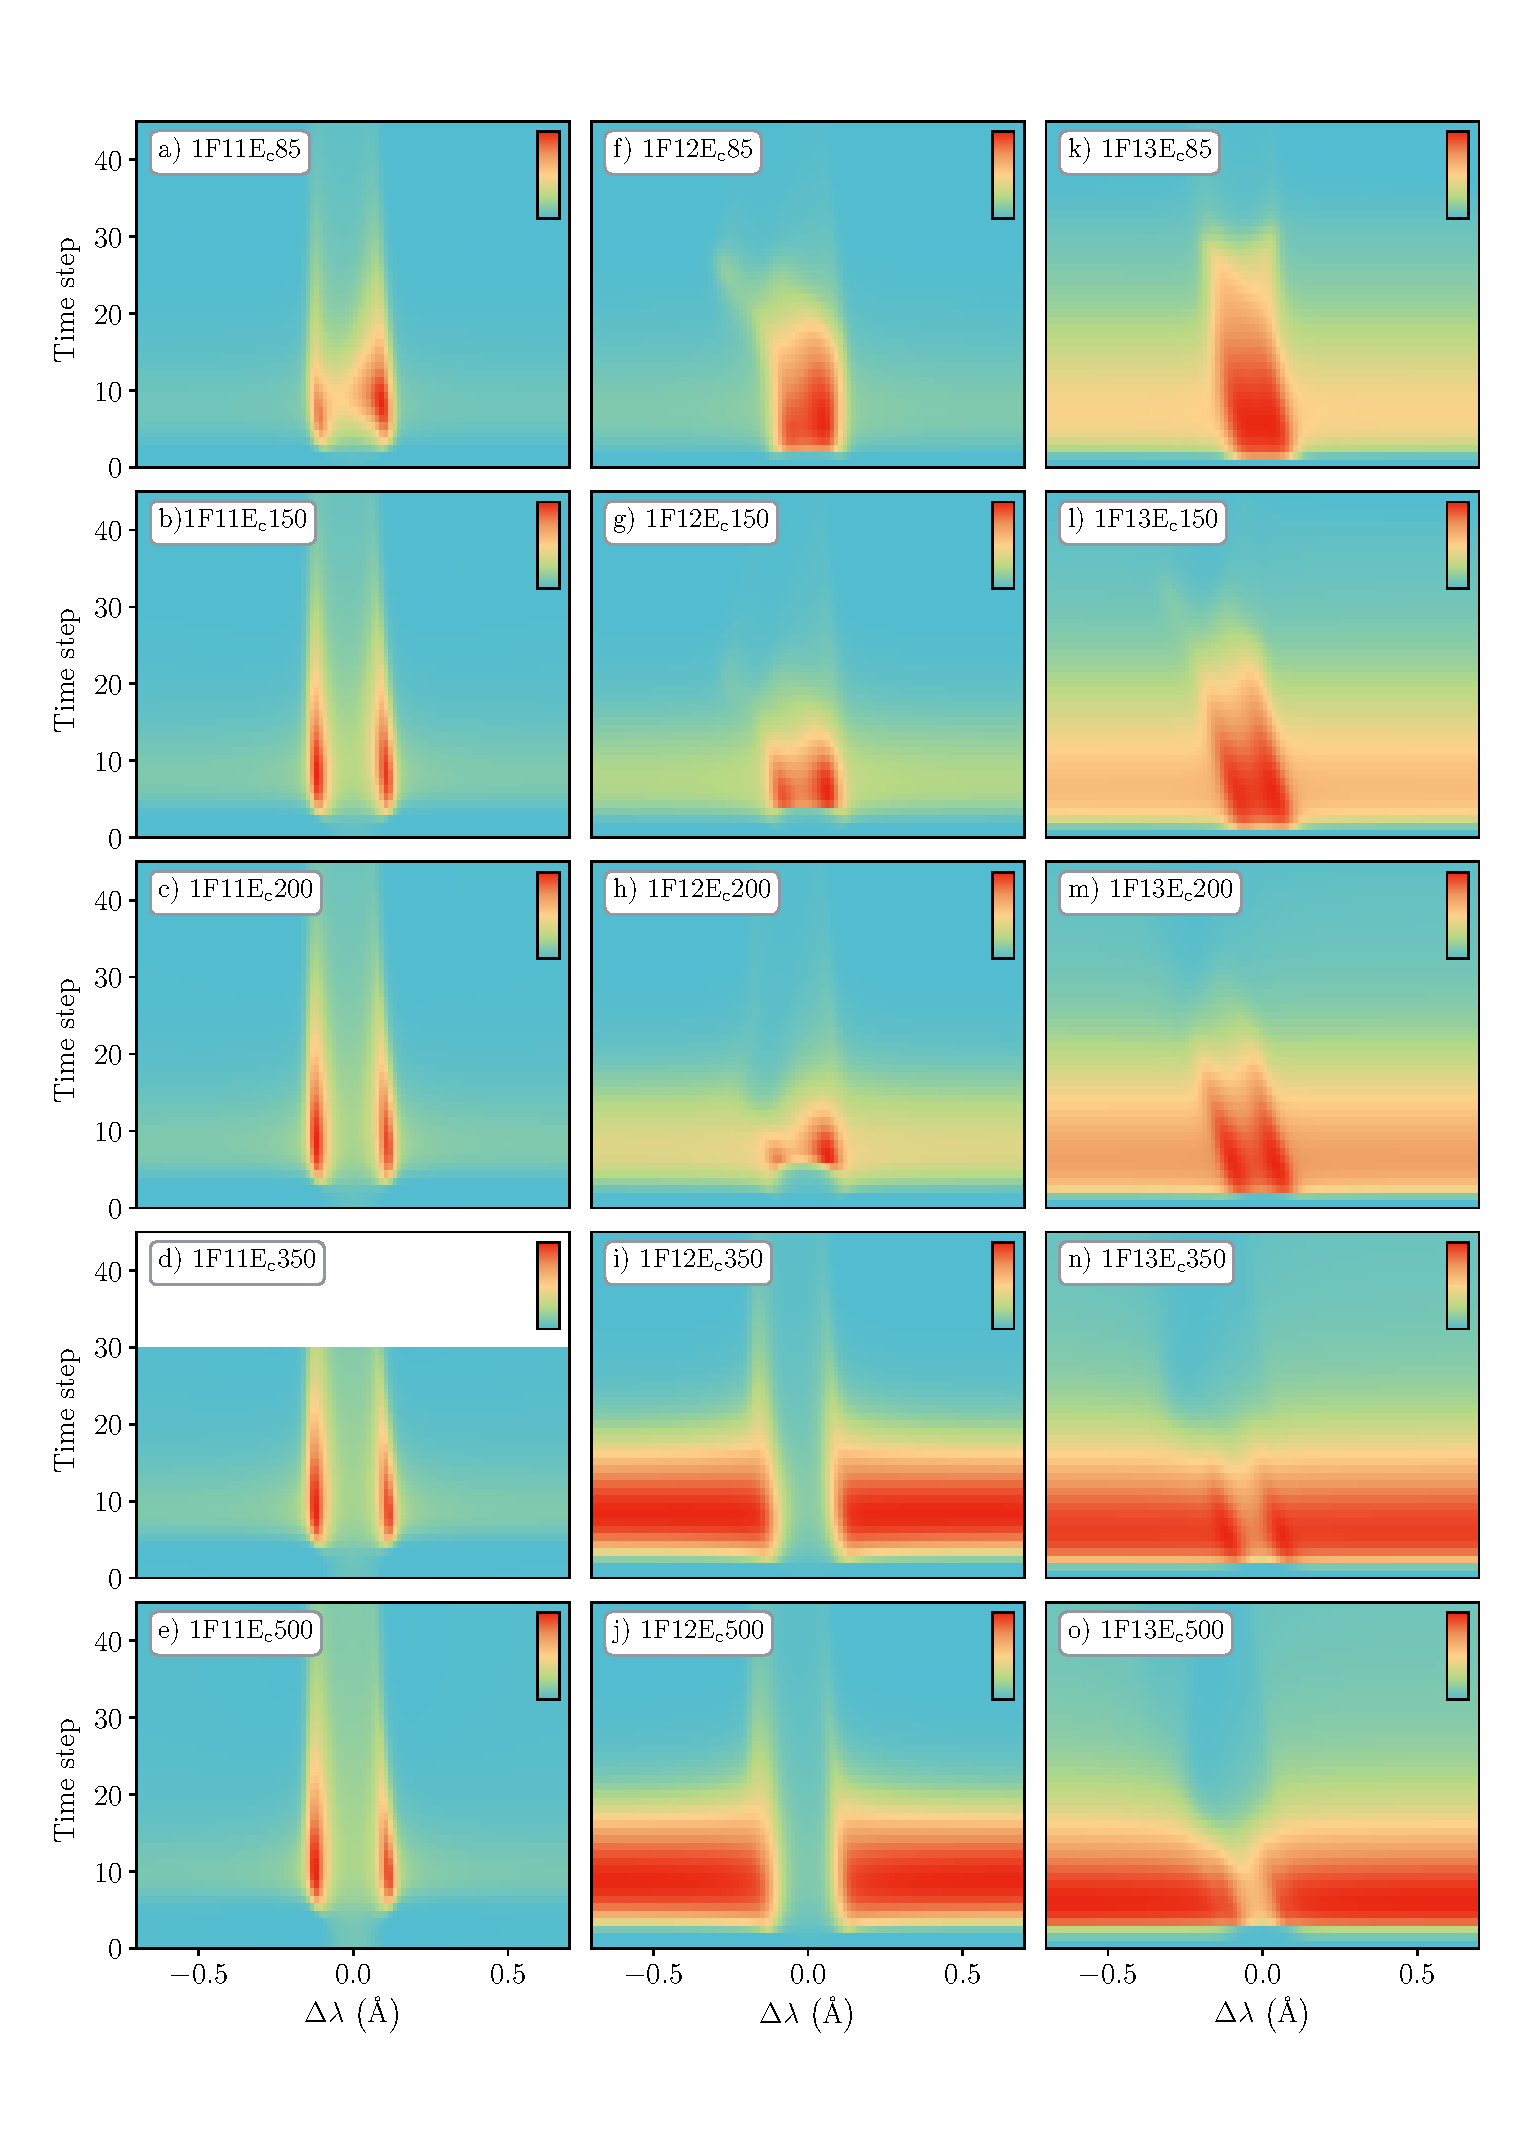
\includegraphics[width=\textwidth]{figs/dMe_MgII_2791}
	\caption{Mg \textsc{ii} 2791 \mbox{\AA}线在不同电子束参数的模拟中的谱线流量随时间演化图。}
	\label{fig:4.6}
\end{figure}

\begin{figure}
	\centering
	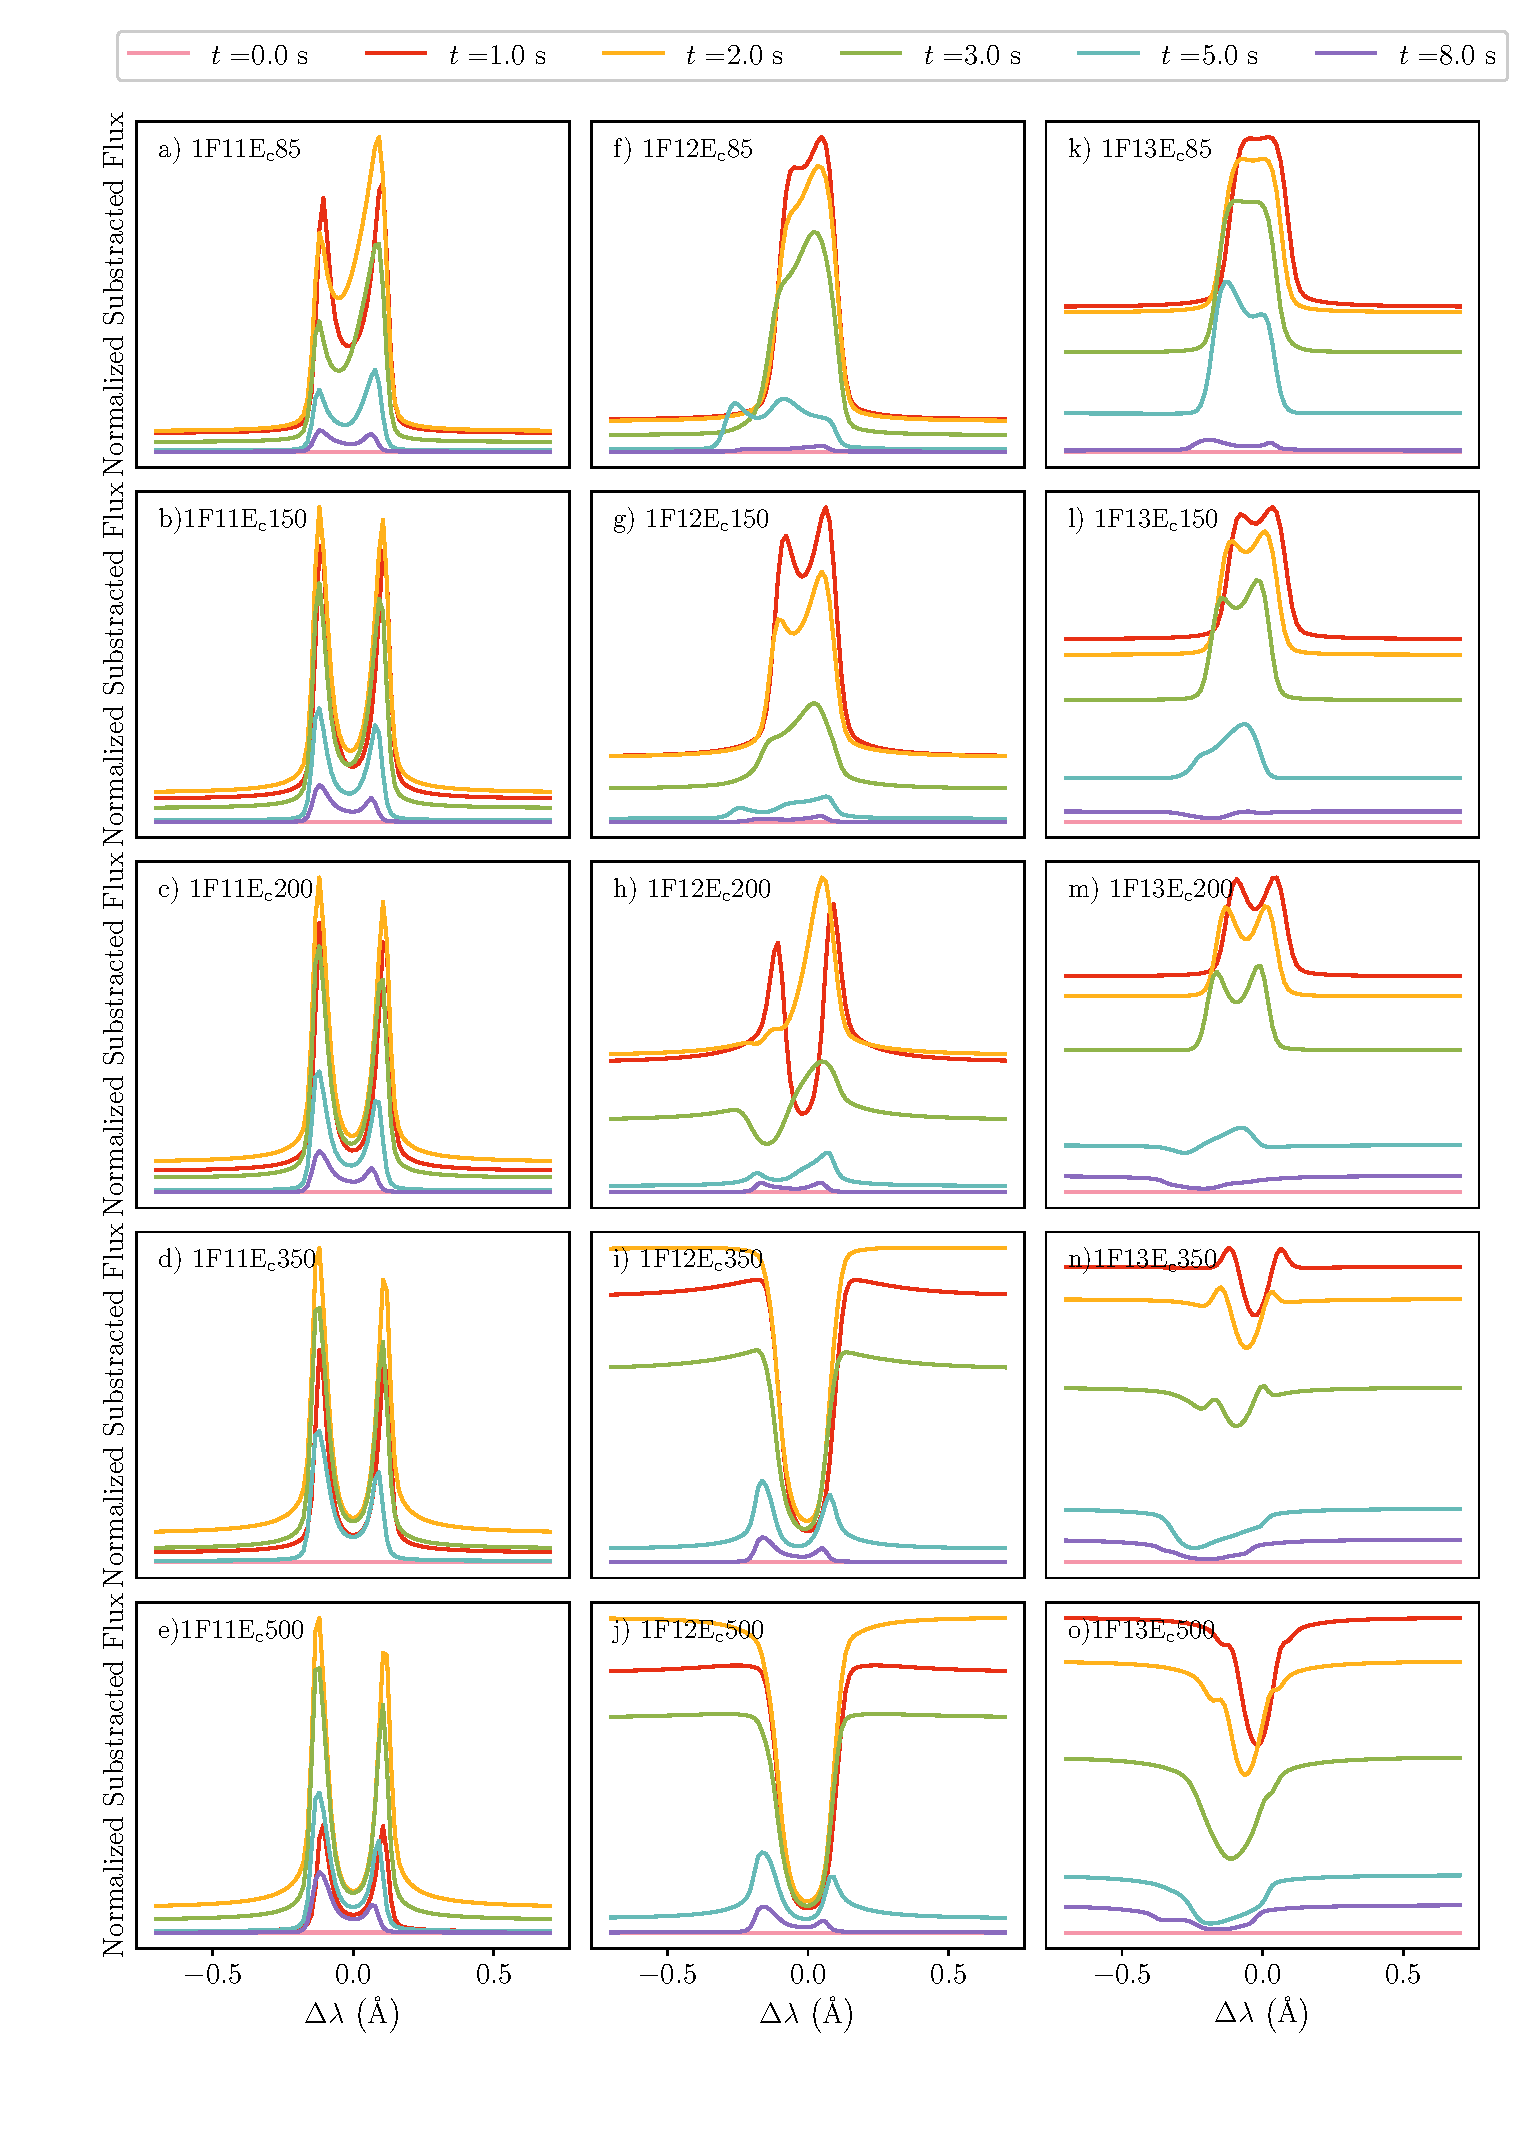
\includegraphics[width=\textwidth]{figs/dMe_MgII2791_spec}
	\caption{Mg \textsc{ii} 2791 \mbox{\AA}线在不同电子束参数的模拟一些特征时刻的谱线轮廓。注意图中展示的是已经减掉宁静初始大气辐射的净辐射流量。}
	\label{fig:4.7}
\end{figure}

和太阳上的Mg \textsc{ii} 2791 \mbox{\AA}有所不同的是,在\ref{sec:4.4}节中我们将会看到Mg \textsc{ii}三重线的线心形成高度事实上是和Mg \textsc{ii} h和k线相当接近的,不同的是Mg \textsc{ii} 三重线的线翼会形成在更深的位置。因此和Mg \textsc{ii} h线类似,三重线的谱线轮廓演化会随高色球和低色球两部分的加热、速度分布不同而表现出不同的轮廓形状。

在1F11模型中,大部分的Mg \textsc{ii} 2791 \mbox{\AA}线的轮廓形状都类似,表现为在线心处没有剧烈增强,但是在靠近线心的两翼有明显增强,而在更远的线翼位置,谱线同样由于Stark致宽而有一定程度的辐射增强。

在1F12和1F13模型中,三重线谱线轮廓变化展现出完全不同的演化特征。在相对较低的截止能量$E_c$时,谱线线心出现的明显的辐射增强,并出现一定程度的红翼增强。在$E_c$较大时,周围连续谱剧烈增强,谱线又重新变为吸收线。




\section{形成高度分析}\label{sec:4.4}

\begin{figure}
	\centering
	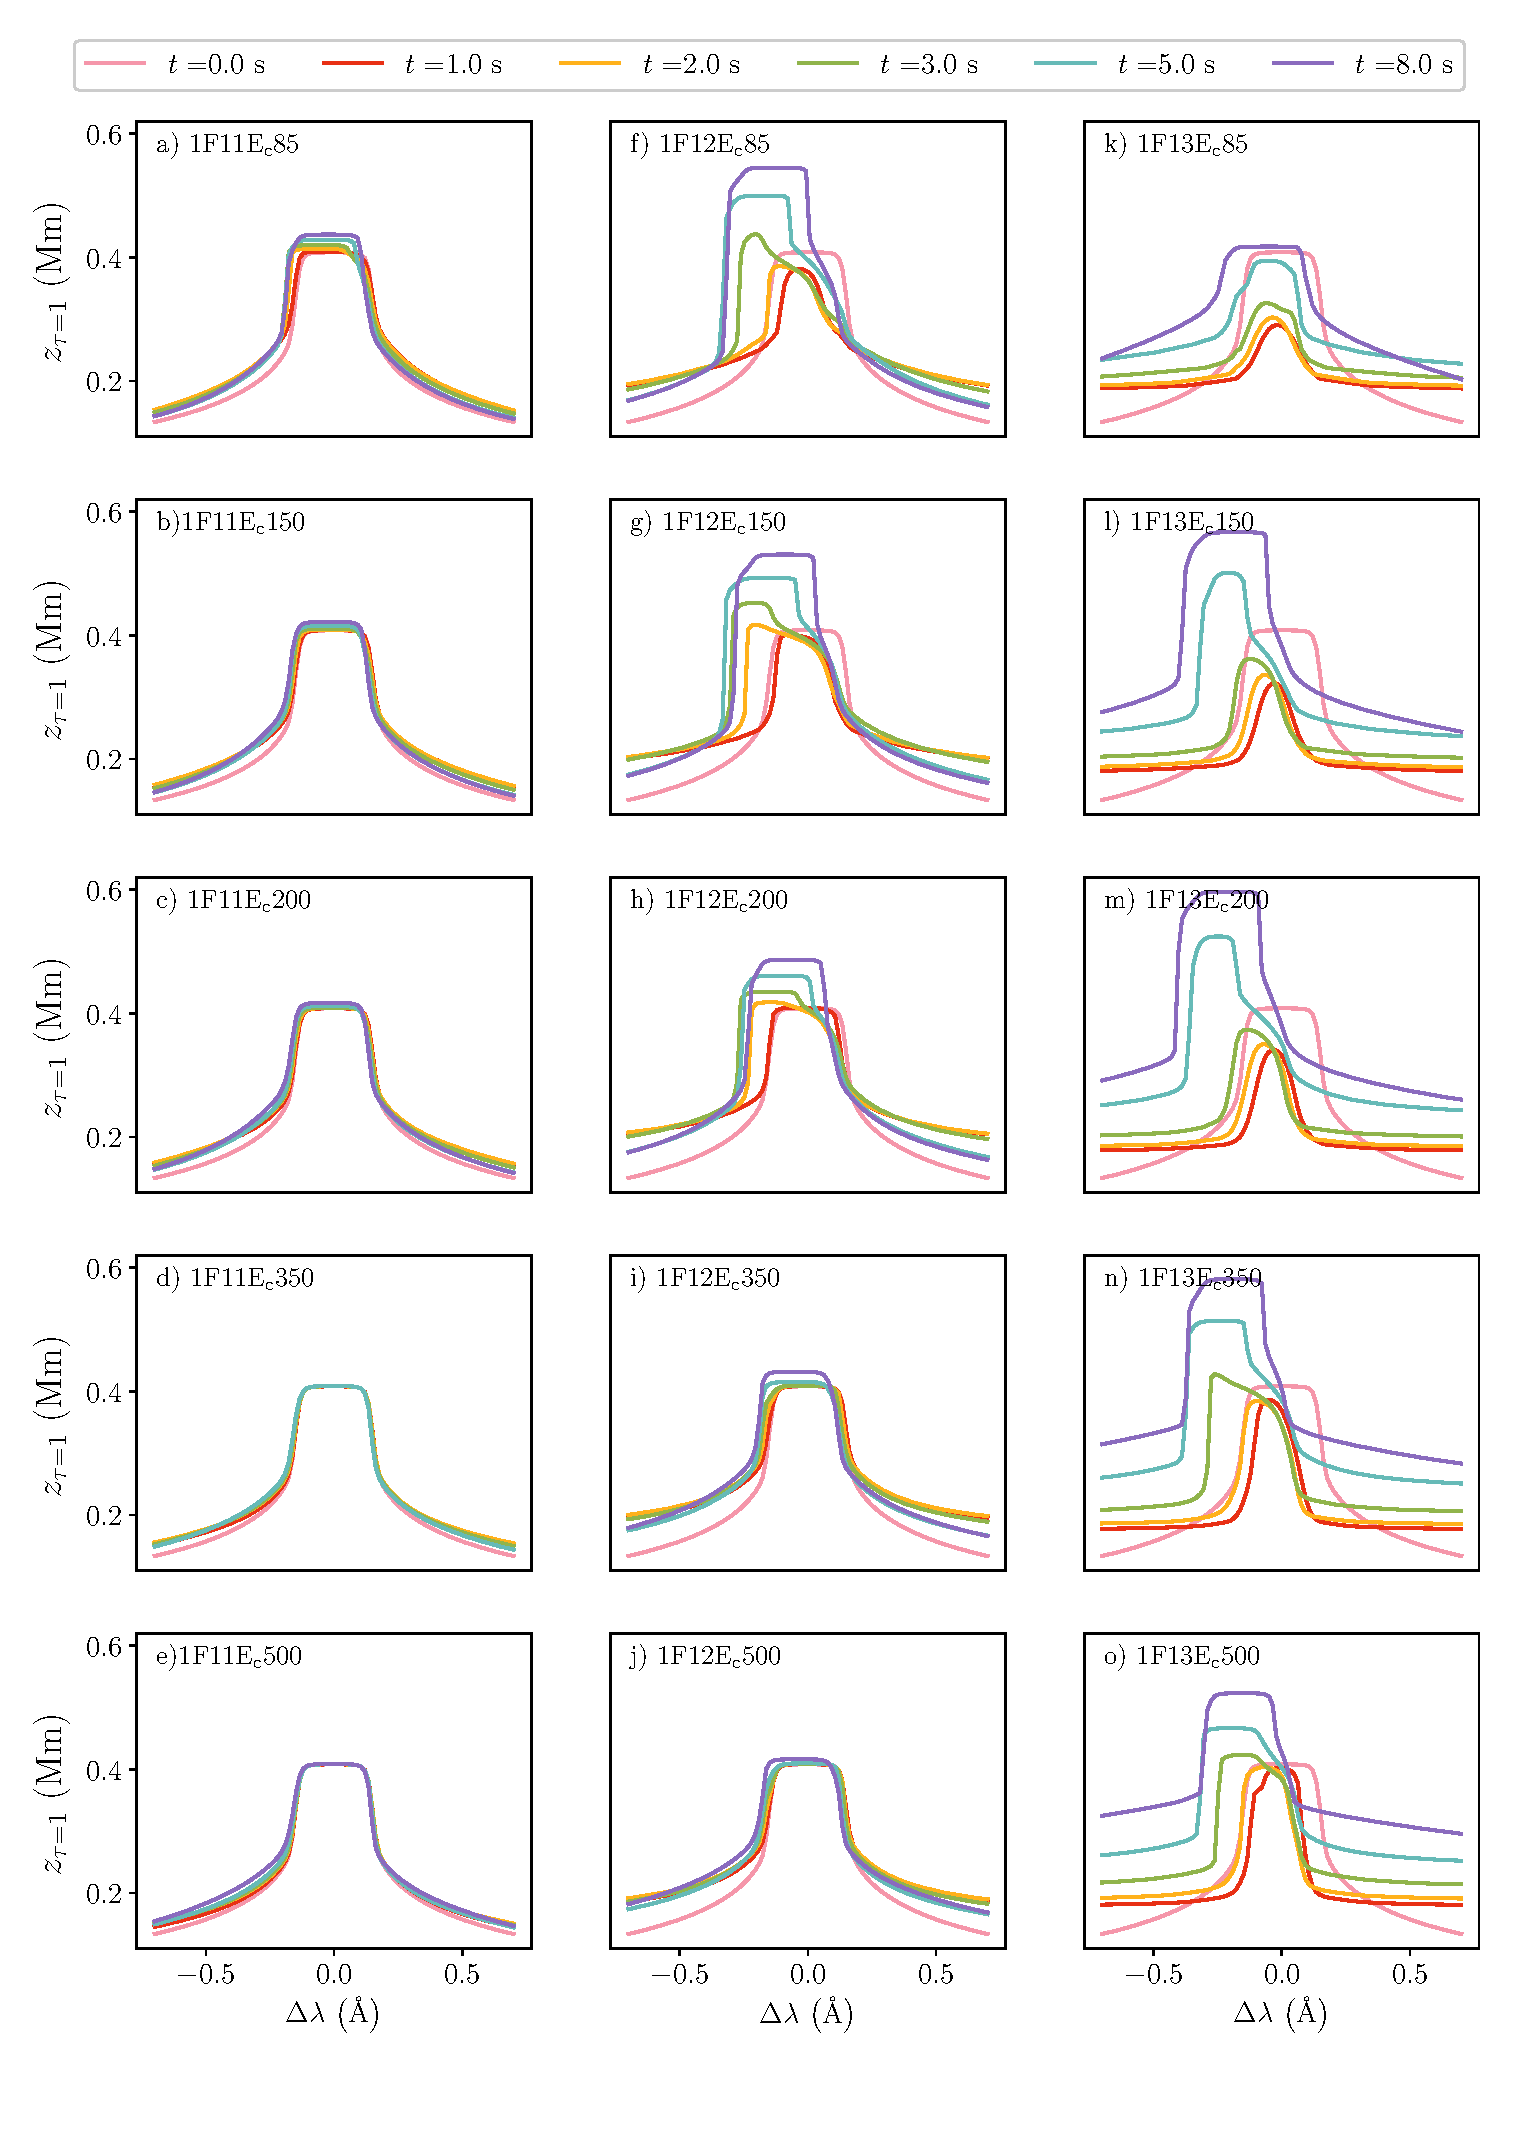
\includegraphics[width=\textwidth]{figs/dMe_MgIIh_tau1}
	\caption{Mg \textsc{ii} h线在不同电子束参数加热情况下谱线范围内的光学深度$\tau = 1$的高度$z_{\tau=1}$随时间演化图。}
	\label{fig:4.8}
\end{figure}

\begin{figure}
	\centering
	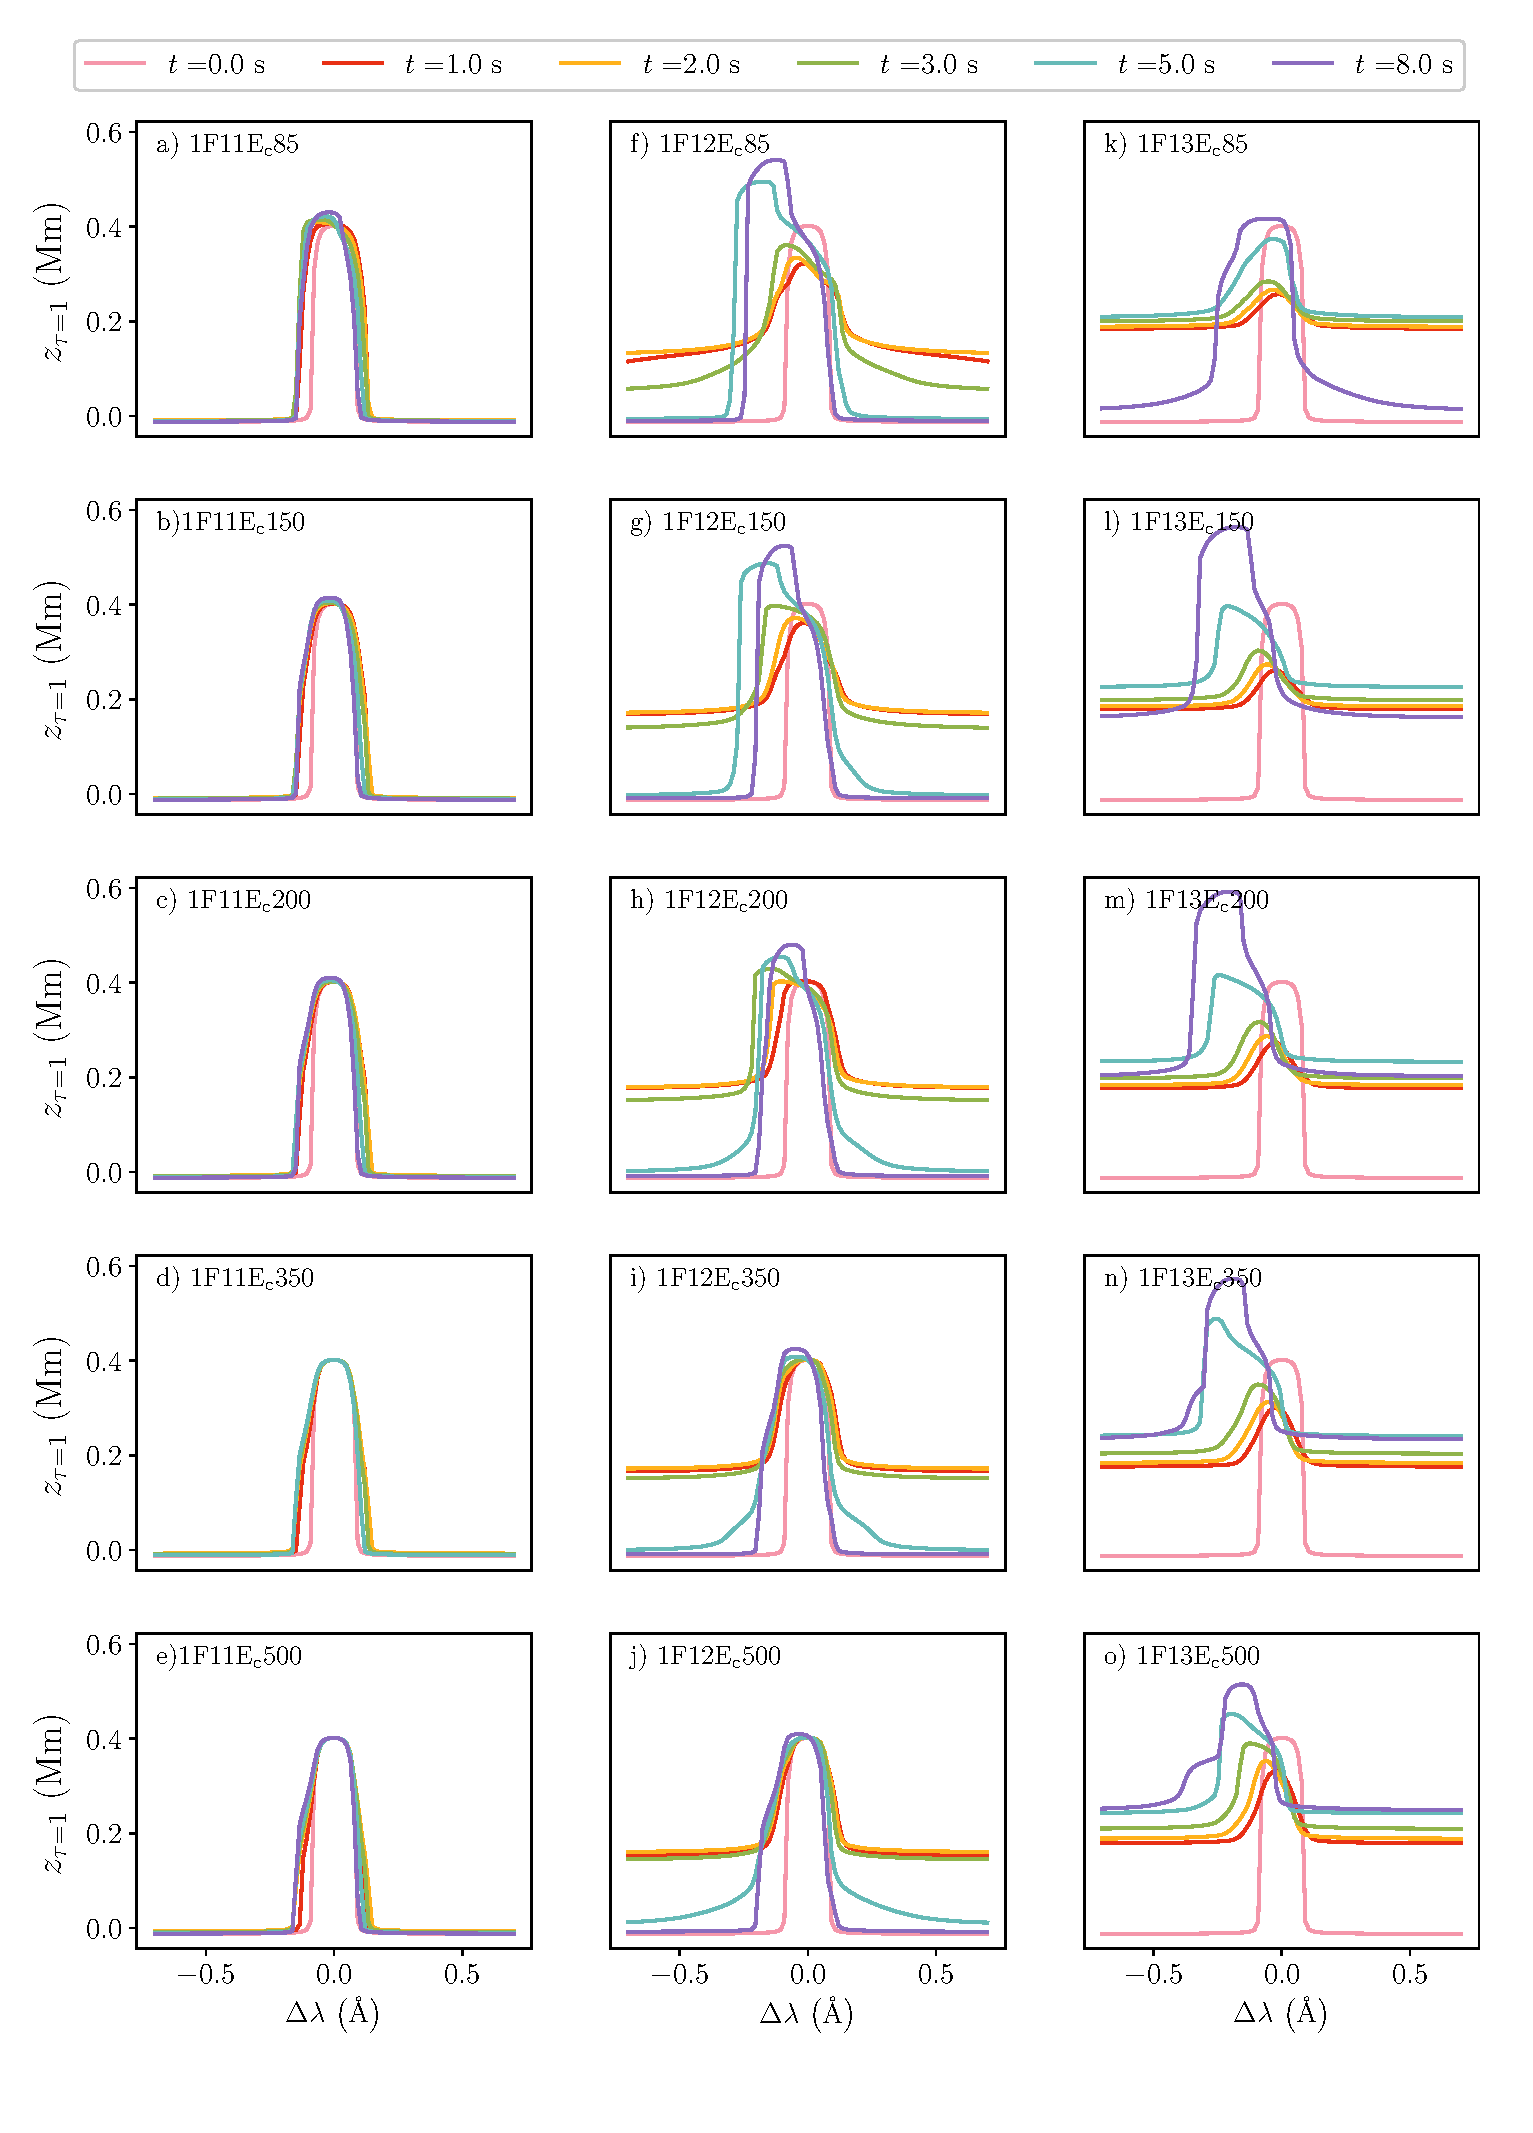
\includegraphics[width=\textwidth]{figs/dMe_MgII2791_tau1}
	\caption{Mg \textsc{ii} 2791 \mbox{\AA}线在不同电子束参数加热情况下谱线范围内的光学深度$\tau = 1$的高度$z_{\tau=1}$随时间演化图。}
	\label{fig:4.9}
\end{figure}

我们在这一节中主要依靠光学深度$\tau_\nu = 1$的对应高度$z_{\tau = 1}$来确定光学厚的Mg \textsc{ii}谱线轮廓在M矮星大气中的形成高度。结合\ref{sec:4.2}中的大气演化参数,对\ref{sec:4.3}节中的一些特征的谱线轮廓的形成做一个简单的解释。图~\ref{fig:4.8}中展示了Mg \textsc{ii} h线轮廓内$\tau_\nu = 1$的高度在之前的特征时刻随波长的分布。一个和太阳大气的明显区别就是在宁静的M矮星大气中,我们发现Mg \textsc{ii} h和k线的线心$\tau = 1$高度和三重线的$\tau = 1$高度比较接近($\sim 0.4 $ Mm)。但三重线的线翼形成在非常低的高度上($\sim 0$ Mm),而Mg \textsc{ii} h和k线线翼形成在相对较高的位置上($\sim 0.2$ Mm)。

在1F11的模型中,所有的Mg \textsc{ii} h和2791 \mbox{\AA}线的形成高度基本没有发生变化。Mg \textsc{ii} h的线翼形成在电子密度约为$10^{14}\ \mathrm{cm^{-3}}$的区域内,因此谱线的Stark致宽非常明显。由于线心形成位置的大气参数几乎没有变化(除了$E_c = 85$ KeV),因此线心强度没有明显变化。而Mg \textsc{ii} 2791 \mbox{\AA}在线心两旁的增强则是来自于低层大气的加热导致的这些频率位置的$\tau = 1$高度上升而靠近线心形成位置,因此这部分的辐射强度因为形成高度温度较高,而明显增强。

在1F12的模型中,Mg \textsc{ii}线和2791三重线的$\tau = 1$层随时间演化和对模型的依赖关系都比较相近,形成的谱线轮廓也有相似之处。相对较小截止能量$E_c$时线心辐射增强而形成的发射线主要来自于上色球部分的加热,其红翼不对称性主要来自于上流物质引起的蓝翼$\tau = 1$层的高度进一步上升,因此蓝翼相对辐射较小,出现红翼不对称性。而在高截止能量的情况下,线心附近的$\tau =1$层并不变化,表现为线心辐射强度基本不变。所有的1F12模型的谱线线翼的形成高度均有所上升,特别是在高截止能量$E_c$的模型中,其线翼形成高度基本和低色球的温度极值区域相重合,因此表现在光谱上是连续谱由于自由电子复合产生的Balmer连续谱辐射。

1F13模型中的情况和1F12模型类似,速度上流造成了谱线蓝翼的$\tau = 1$高度抬升,且整个谱线都出现了整体的蓝移。在$E_c = 350$ KeV的模型中Mg \textsc{ii} h线出现红翼发射但蓝翼吸收的净谱线轮廓主要来自于在过渡区下方的温度结构存在一段温度随高低降低的情况,而蓝翼抬升的谱线形成高度导致了蓝翼发射的不足,因此看上去和增强的红翼和连续谱部分相比,蓝翼部分更类似于吸收。同样的所有的线翼形成高度都有一定程度的上升,2791 \mbox{\AA}线线翼的形成高度大约在0.2 Mm左右,而Mg \textsc{ii} h的线翼有进一步抬升的趋势,在高截止能量的模型中可以达到0.3 Mm。



\section{讨论}
\textcites{Hawley2007}利用HST/STIS对一颗M矮星YZ CMi上爆发的多个耀斑的Mg \textsc{ii}线进行了观测,这些谱线都表现出增强和剧烈致宽的特征,如果用Doppler速度来衡量这些谱线的致宽,它们的半高全宽将会达到$250\ \mathrm{km\  s^{-1}}$以上。她们对其中两个比较大的耀斑事件的净谱线轮廓进行了研究,如图~\ref{fig:4.10}。其中F2事件所展示的Mg \textsc{ii}光谱演化是先出现蓝翼增强,然后再逐渐减弱。而F9事件则恰恰相反,先出现的是红翼增强,再逐渐减弱。为了能够更好的对比HST/STIS曝光时间较长的观测数据,我们对各个模拟中的谱线轮廓对时间进行了平均,平均后的净辐射流量展示在图~\ref{fig:4.11}中。

在我们的参数空间中,只有1F11$E_c85$模型的平均净辐射流量能够表现出一定的蓝翼增强,而只有1F13$E_c350$的平均净辐射流量能够表现出一定的红翼增强。而在拟合白光连续谱上表现最好的1F13$E_c85$模型得到的是和普通太阳类似的发射谱线。考虑到整个参数空间中的耀斑模型已经能够覆盖目前观测到的M矮星耀斑中的大多数Balmer跳跃比、H$\gamma$/C4170等白光谱附近的特征,我认为目前不能找到拟合的非常好的谱线轮廓的主要原因还是在于一维辐射流体力学的模拟对耀斑过程中复杂的色球大气动力学过程不能进行很好的再现。从模拟的角度上来看,连续谱的形成范围更宽,且涉及的复杂的物理过程更少。对于谱线轮廓的模拟而言,必须对整个大气的结构有相当深入且精确的认识,同时我们需要对涉及谱线形成的复杂物理过程都有一个相对准确的近似,才能更好地利用辐射转移模拟来实现光学厚谱线诊断提供依据。

\begin{figure}
	\centering
	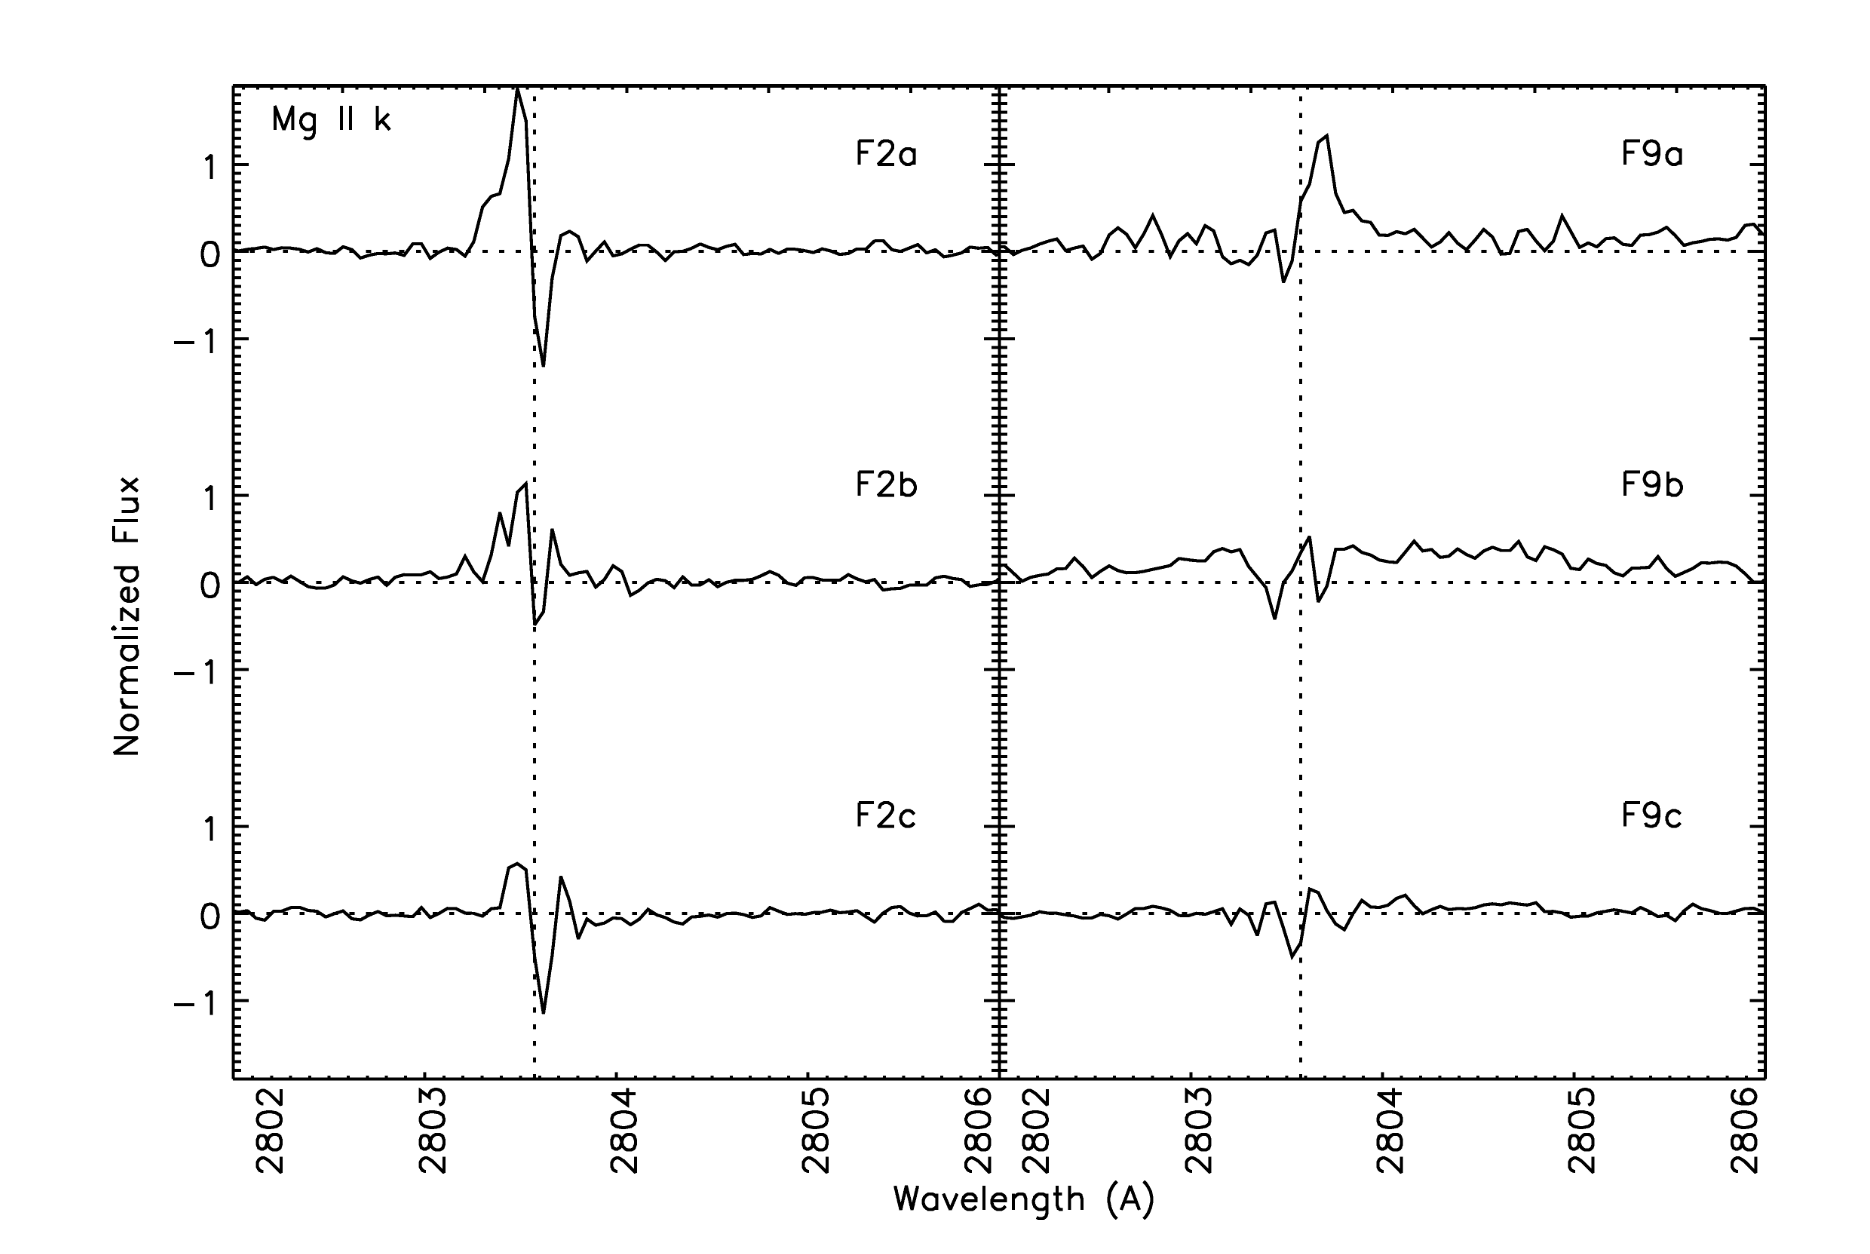
\includegraphics[width=0.5\textwidth]{figs/Hawley2007}
	\caption{两个M矮星上的大耀斑中观测到的Mg \textsc{ii} k线净轮廓。来源:\textcites{Hawley2007}}
	\label{fig:4.10}
\end{figure}

\begin{figure}
	\centering
	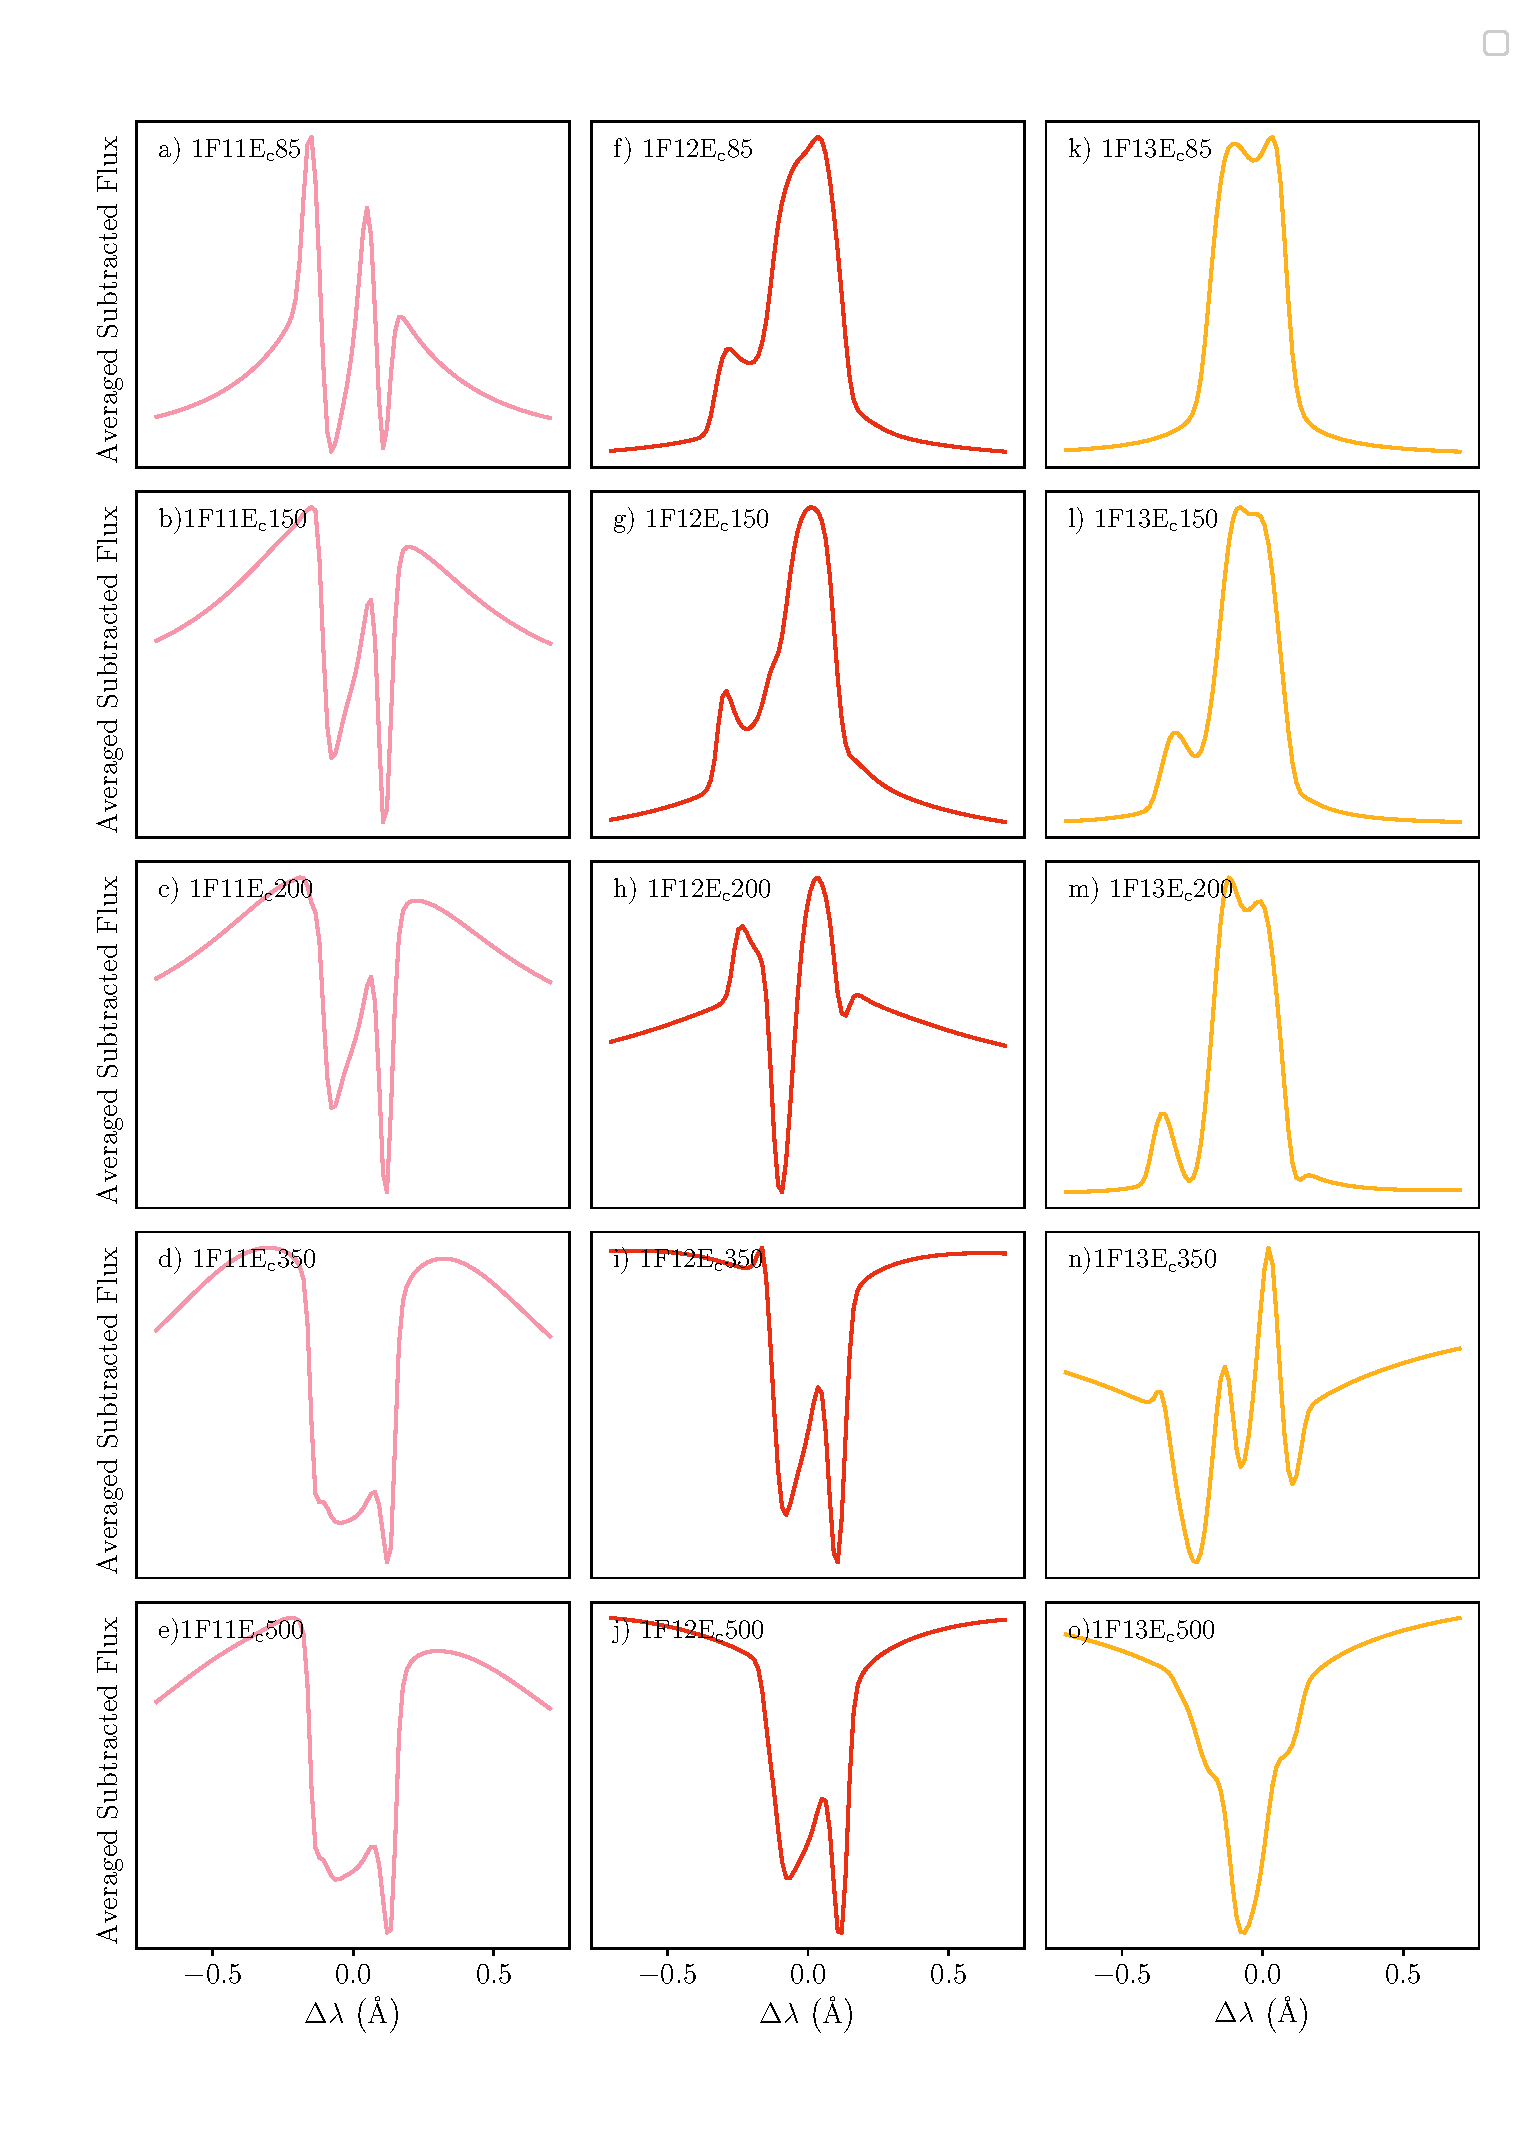
\includegraphics[width=\textwidth]{figs/dMe_MgIIh_spec_aver}
	\caption{Mg \textsc{ii} h线在不同电子束参数加热情况下对整个模拟过程取平均后的净辐射流量(已经减去初始宁静大气的辐射)。}
	\label{fig:4.11}
\end{figure}





% vim:ts=4:sw=4
	% Copyright (c) 2014,2016 Casper Ti. Vector
% Public domain.

\chapter{谱线对低高度小尺度加热的响应}\label{chap:5}
在这一章节中我们利用RH代码对太阳上低高度、小尺度的加热现象产生的Mg \textsc{ii}线和H$\alpha$线进行模拟。之所以不使用IRIS另外观测的C \textsc{ii}线和Si \textsc{iv}线的原因是C \textsc{ii}线存在计算时的数值崩溃或不能收敛的问题,可能来自于某些高温大气造成的原子能级粒子数在LU分解中产生奇异性。而Si \textsc{iv}线已经在\ref{sec:3.8}节中的讨论中证明不包含Si \textsc{i}和\textsc{ii}能级的Si原子文件不适合对Si \textsc{iv}谱线的形成进行模拟。因此我们把目光投向Mg \textsc{ii}线和H$\alpha$线,计算在低高度出现小尺度加热时的谱线轮廓变化。
\section{研究方法}
为了研究的方便,我们在这里仅采取一种半经验的方法,通过人工在RH的输入大气中在低高度上的几个格点的温度进行修改。整个插入过程依靠的是我自己临时编写的一个可视化ipython小程序(见~\ref{sec:a.1.3})。同时我们没有给RH代码输入电子密度随高度的分布,故其将自动根据我们的提供的温度信息迭代计算该高度上的NLTE电离下的电子密度。在得到RH代码计算的谱线之后,我们将这些谱线和紫外爆发以及Ellerman炸弹的典型光谱进行比较,希望能够寻找到拟合较好的谱线轮廓,帮助我们更好地认识这些在色球,乃至光球层次上的小尺度加热过程。
\section{初始设置}
我在宁静太阳VALC大气的五个高度点0.25, 0.5, 0.75, 1.0和1.5 Mm上分别尝试插入了一些温度比原有温度高$2\times10^3-4\times10^5$ K不等的温度,具体插入的数值可以参见表~\ref{Table2}和图~\ref{fig:5.1}。注意图~\ref{fig:5.1}中的电子密度$n_e$已经是经过RH代码计算后的结果。显然插入一个局域的温度上升能够提高局地的电子密度,而且插入的位置温度越低,相同的温度升高反而能导致更多的H \textsc{i}原子电离,产生相对更大的电子密度增加。此外值得一提的一点是为了简化操作量我并没有在响应的高度上插入速度的双向流。这对较低高度上的Ellerman炸弹的模拟可能并无太大影响,因为在光球小尺度的加热并不会产生非常大的宏观体速度流\parencites{Hong2017b}。而对于发生在较高高度的紫外爆发,它们一般会形成较大的速度流和较宽的谱线轮廓。

\begin{table}
	\centering
	\begin{tabular}{cccc}
	\hline
    高度 (Mm) & 温度1 (kK) & 温度2 (kK) & 温度3 (kK)  \\ 
 	\hline
    0.25 & 6 & 8 & 10 \\
    0.50 & 6 & 8 & 10\\
    0.75 & 6 & 10 & 20 \\
    1.00 & 8 & 15 & 20 \\
    1.50 & 10 & 20 & 50 \\
    \hline
\end{tabular}
    \caption{本实验中插入温度的数值和其插入高度}\label{Table2}
\end{table}

\begin{figure}
	\centering
	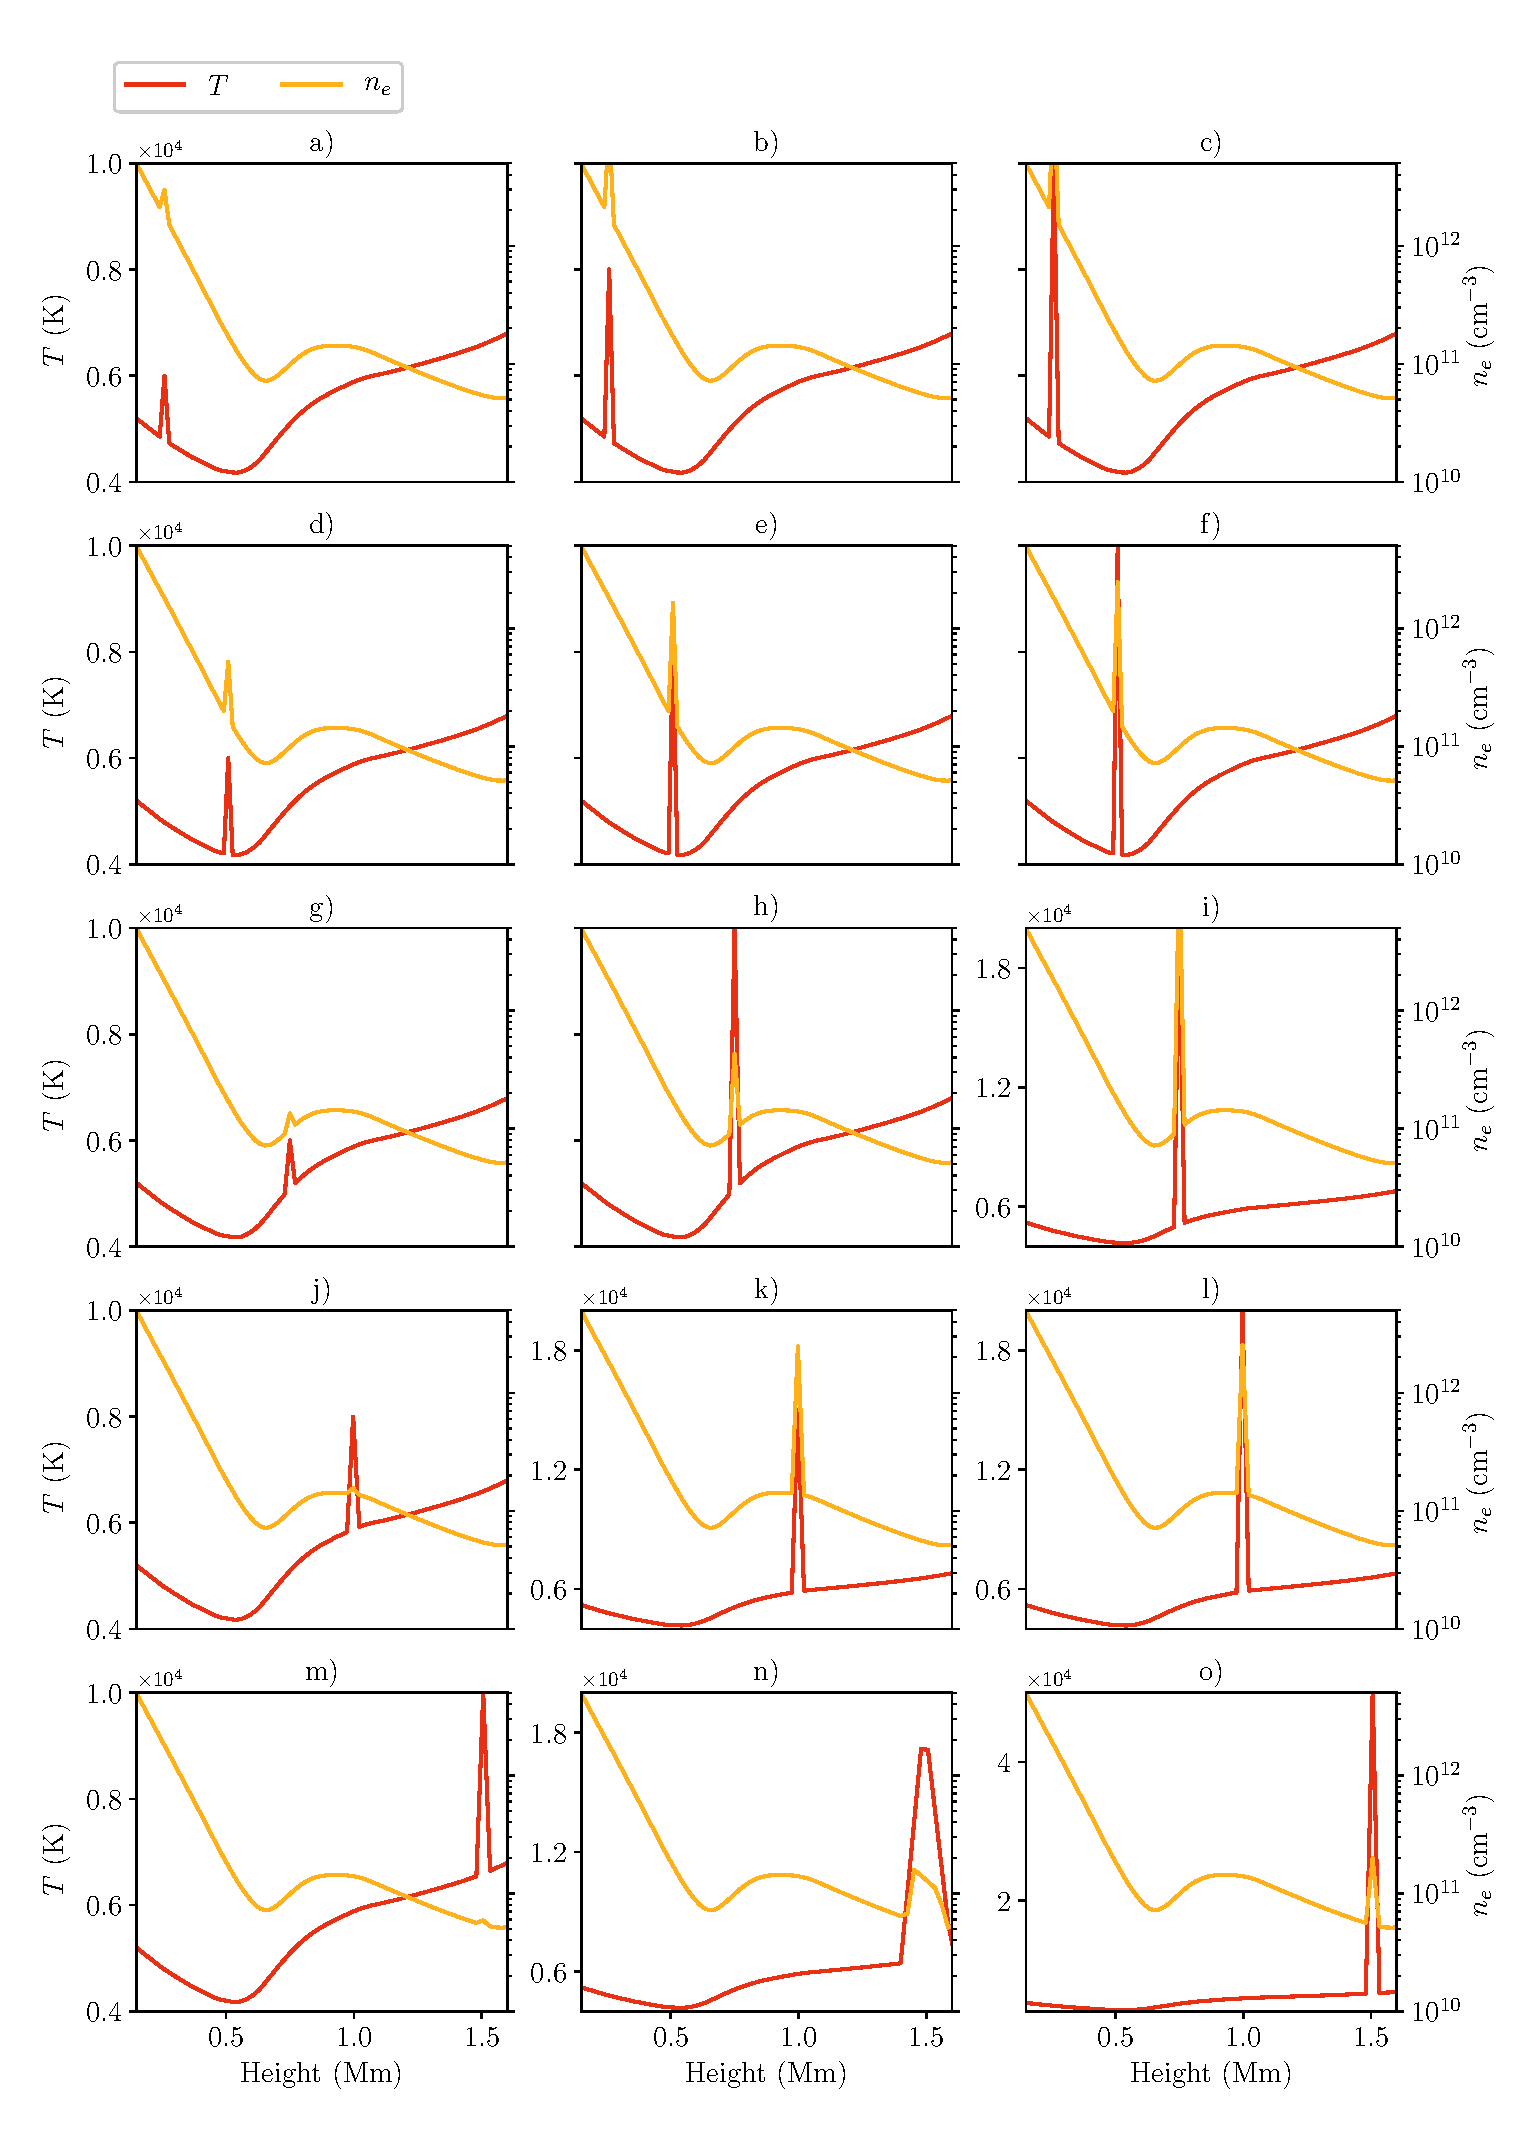
\includegraphics[width=\textwidth]{figs/UVB_atoms}
	\caption{模拟中所使用的经过手动插入温度后的大气模型中温度$T$与电子密度$n_e$随高度的分布。注意其中的电子密度已经是经过RH代码计算后的结果。}
	\label{fig:5.1}
\end{figure}
\section{合成光谱与讨论}在这一部分我们将集中展示在各个大气中计算得到的光谱和实际观测到的光谱的比较。从图~\ref{fig:5.2},\ref{fig:5.3}和\ref{fig:5.4}中可以看到,不同高度不同程度的温度增加,得到了轮廓各异的Mg \textsc{ii}线和H$\alpha$线。在这里,我们不妨对生成的这些谱线对应的大气加热模型的特点做一些归纳:
\begin{enumerate}
	\item 三条谱线都没有明显增强的有a、d、g、j和m栏。这些大气模型的特点就是温度增加不够大,因此无法对周边的原子能级占据数和谱线形成产生影响。
	\item Mg \textsc{ii} h线翼都明显增强的大气模型有c、e、i、f、h、k和l栏。它们的突出特征是在0.25 Mm和1 Mm之间有接近$10^4$ K的温度。
	\item Mg \textsc{ii} 2791 \mbox{\AA}在此时体现出其对低层大气加热的敏感性,较小程度的低层大气加热或只加热高层大气,都不会反映在在Mg \textsc{ii} 2791 \mbox{\AA}谱线轮廓变化上。其线翼增强与Mg \textsc{ii} h线翼的增强保持了比较高的一致性且与观测光谱在线心部分能够得到比较好的拟合。但在低色球加热时整个谱线轮廓并不是\textcites{Pereira2015}中所提到的出现发射线,而仍是伴随着线翼增强的吸收线。
	\item 部分在Mg \textsc{ii} h远线翼出现增强的模型,如b和c,对应着在光球高度发生的局部温度增加。在它们的H$\alpha$合成光谱中,增加温度较小(到约$\sim 8$ kK)的模型出现了$H\alpha$谱线线心和线翼位置的辐射减小,而增加到$10$ kK的模型出现了线心和线翼(主要是在线翼)的辐射增强。这和\textcites{Hong2017b}中对Ellerman炸弹进行数值模拟发现在开始阶段H$\alpha$谱线出现整个谱线轮廓内的辐射减小相类似。尽管这个效应还没有被观测证实,但说明可能存在这样的减弱再增强的过程。
	\item 部分在高色球加热的模型,如k、l出现了Mg \textsc{ii} h线心和H$\alpha$线心线翼位置的增强。这与\textcites{Hansteen2017}中部分Ellerman炸弹和紫外爆发的谱线类似。但与实际观测还存在着一定差距。
	\item 大部分模拟都很难得到和观测非常相似的Mg \textsc{ii} h谱线轮廓,这些轮廓可能来自于模拟中尚未添加的加热区域的宏观速度出流。

\end{enumerate}




\begin{figure}
	\centering
	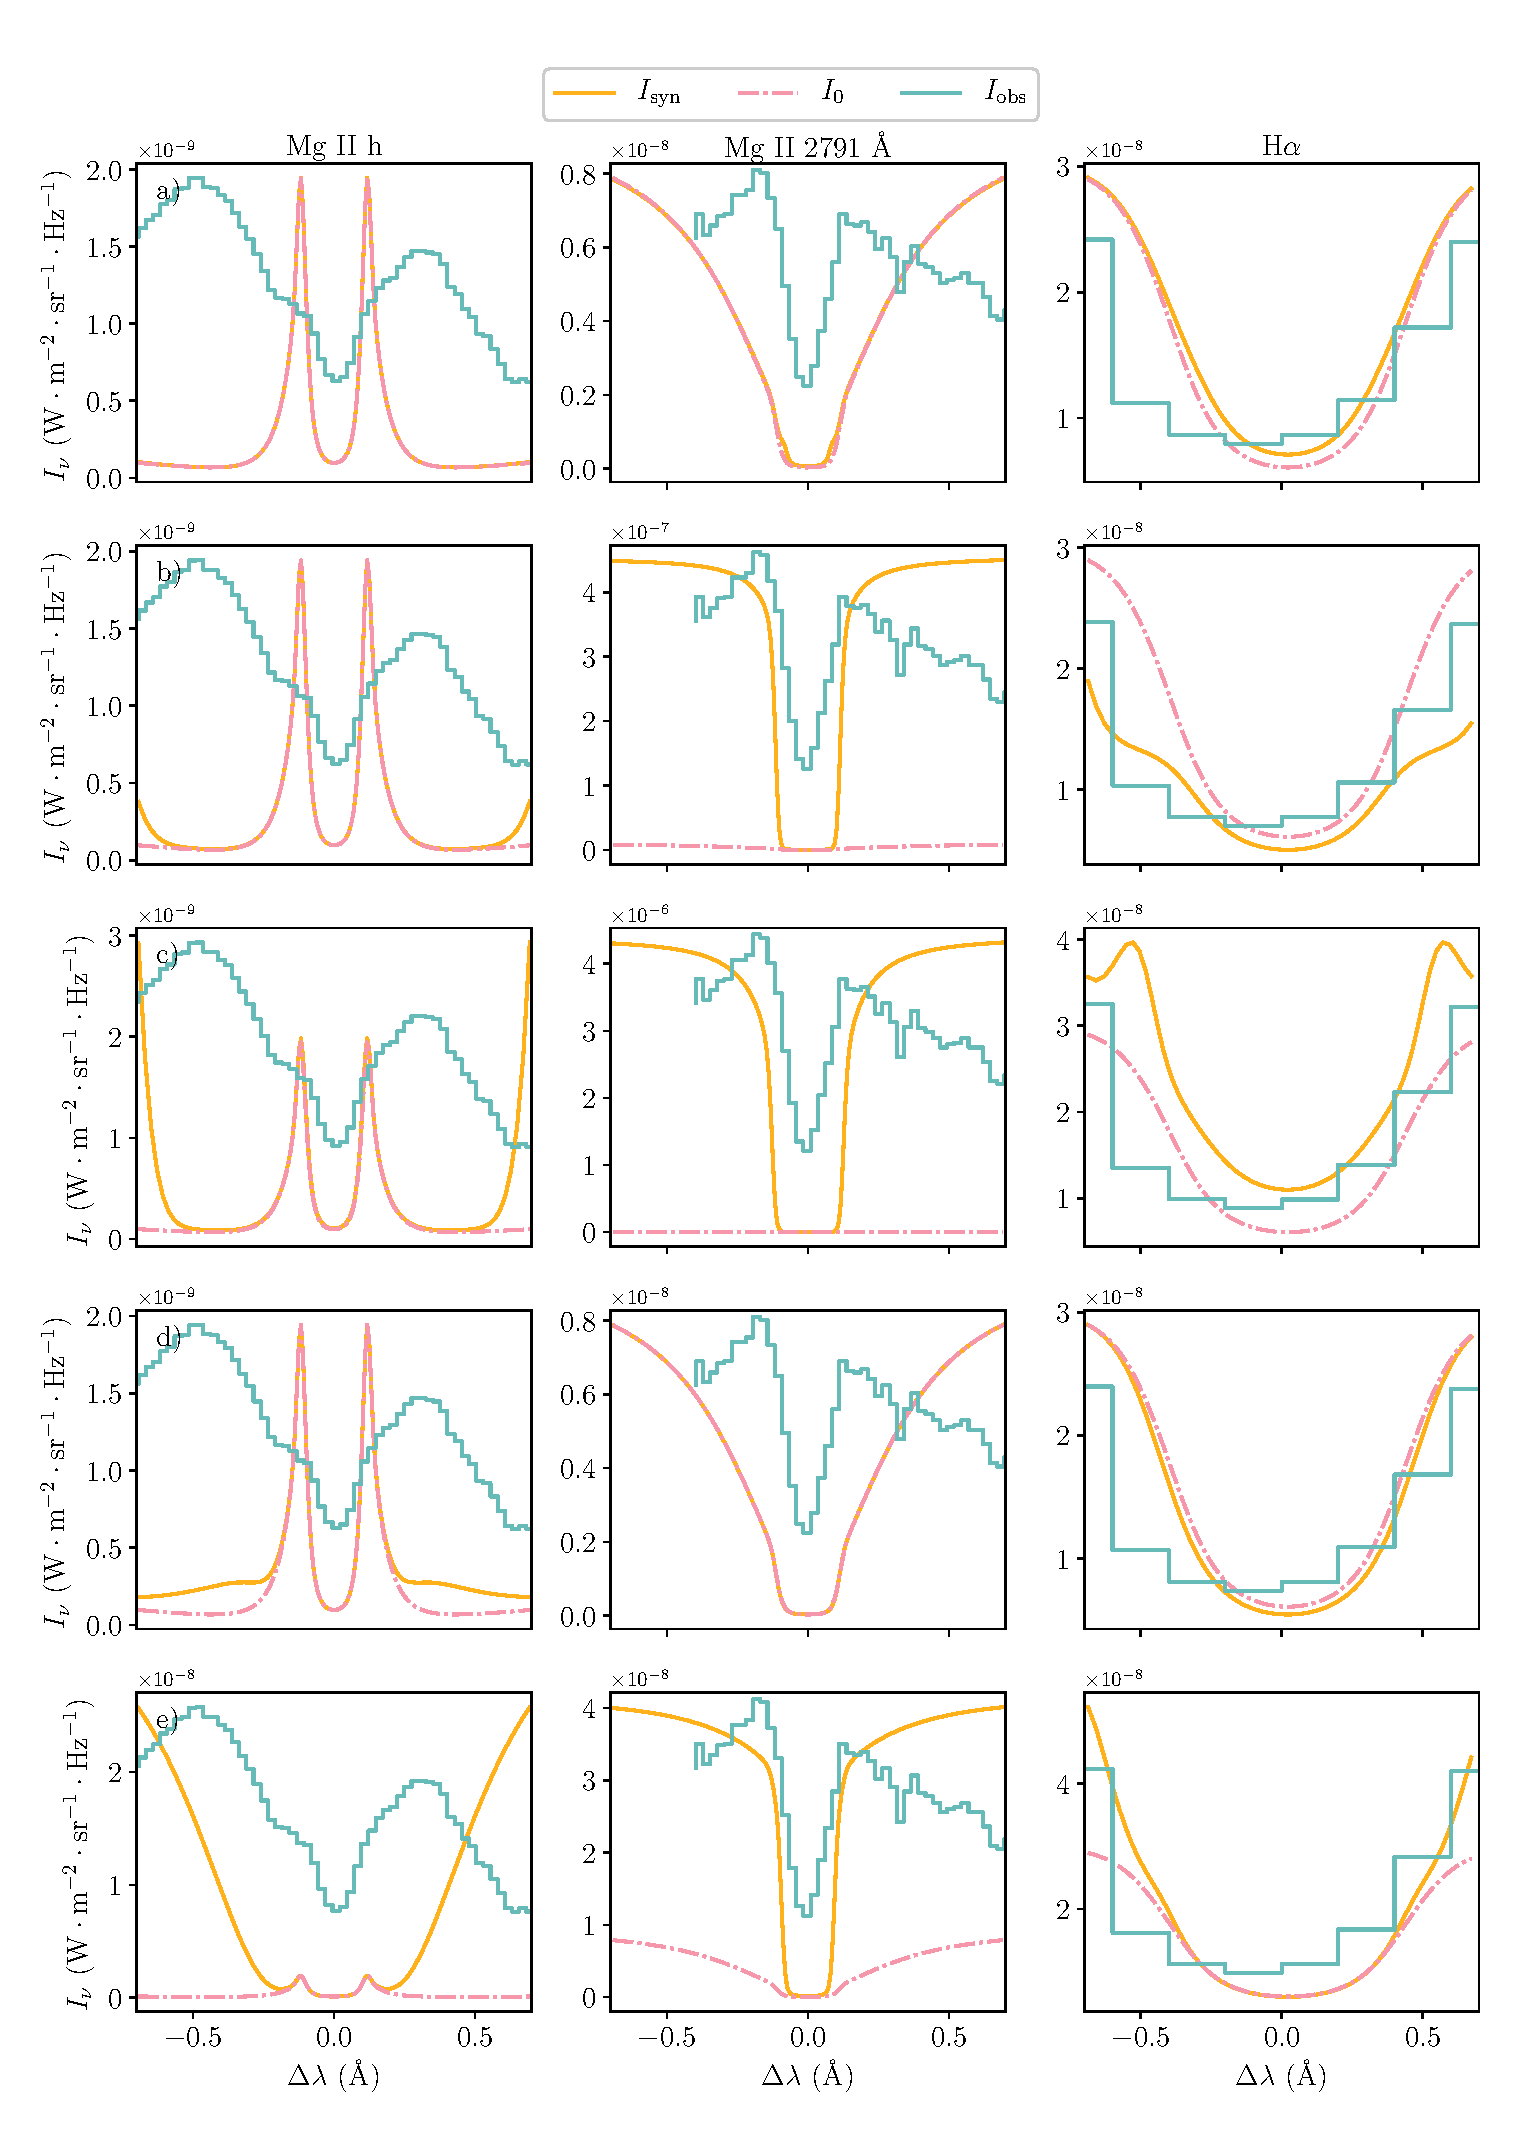
\includegraphics[width=\textwidth]{figs/UVB_spec_1}
	\caption{RH代码模拟得到的低层大气加热后的Mg \textsc{ii} h,2791 \mbox{\AA}及H$\alpha$线的谱线轮廓与IRIS卫星等观测的对比图(其一)。粉色点划线轮廓代表了初始谱线轮廓;黄色实线代表调整后计算得到的谱线轮廓。蓝色阶梯线代表实际观测的紫外爆发(Mg \textsc{ii})和Ellerman炸弹(H$\alpha$)的谱线轮廓。}
	\label{fig:5.2}
\end{figure}

\begin{figure}
	\centering
	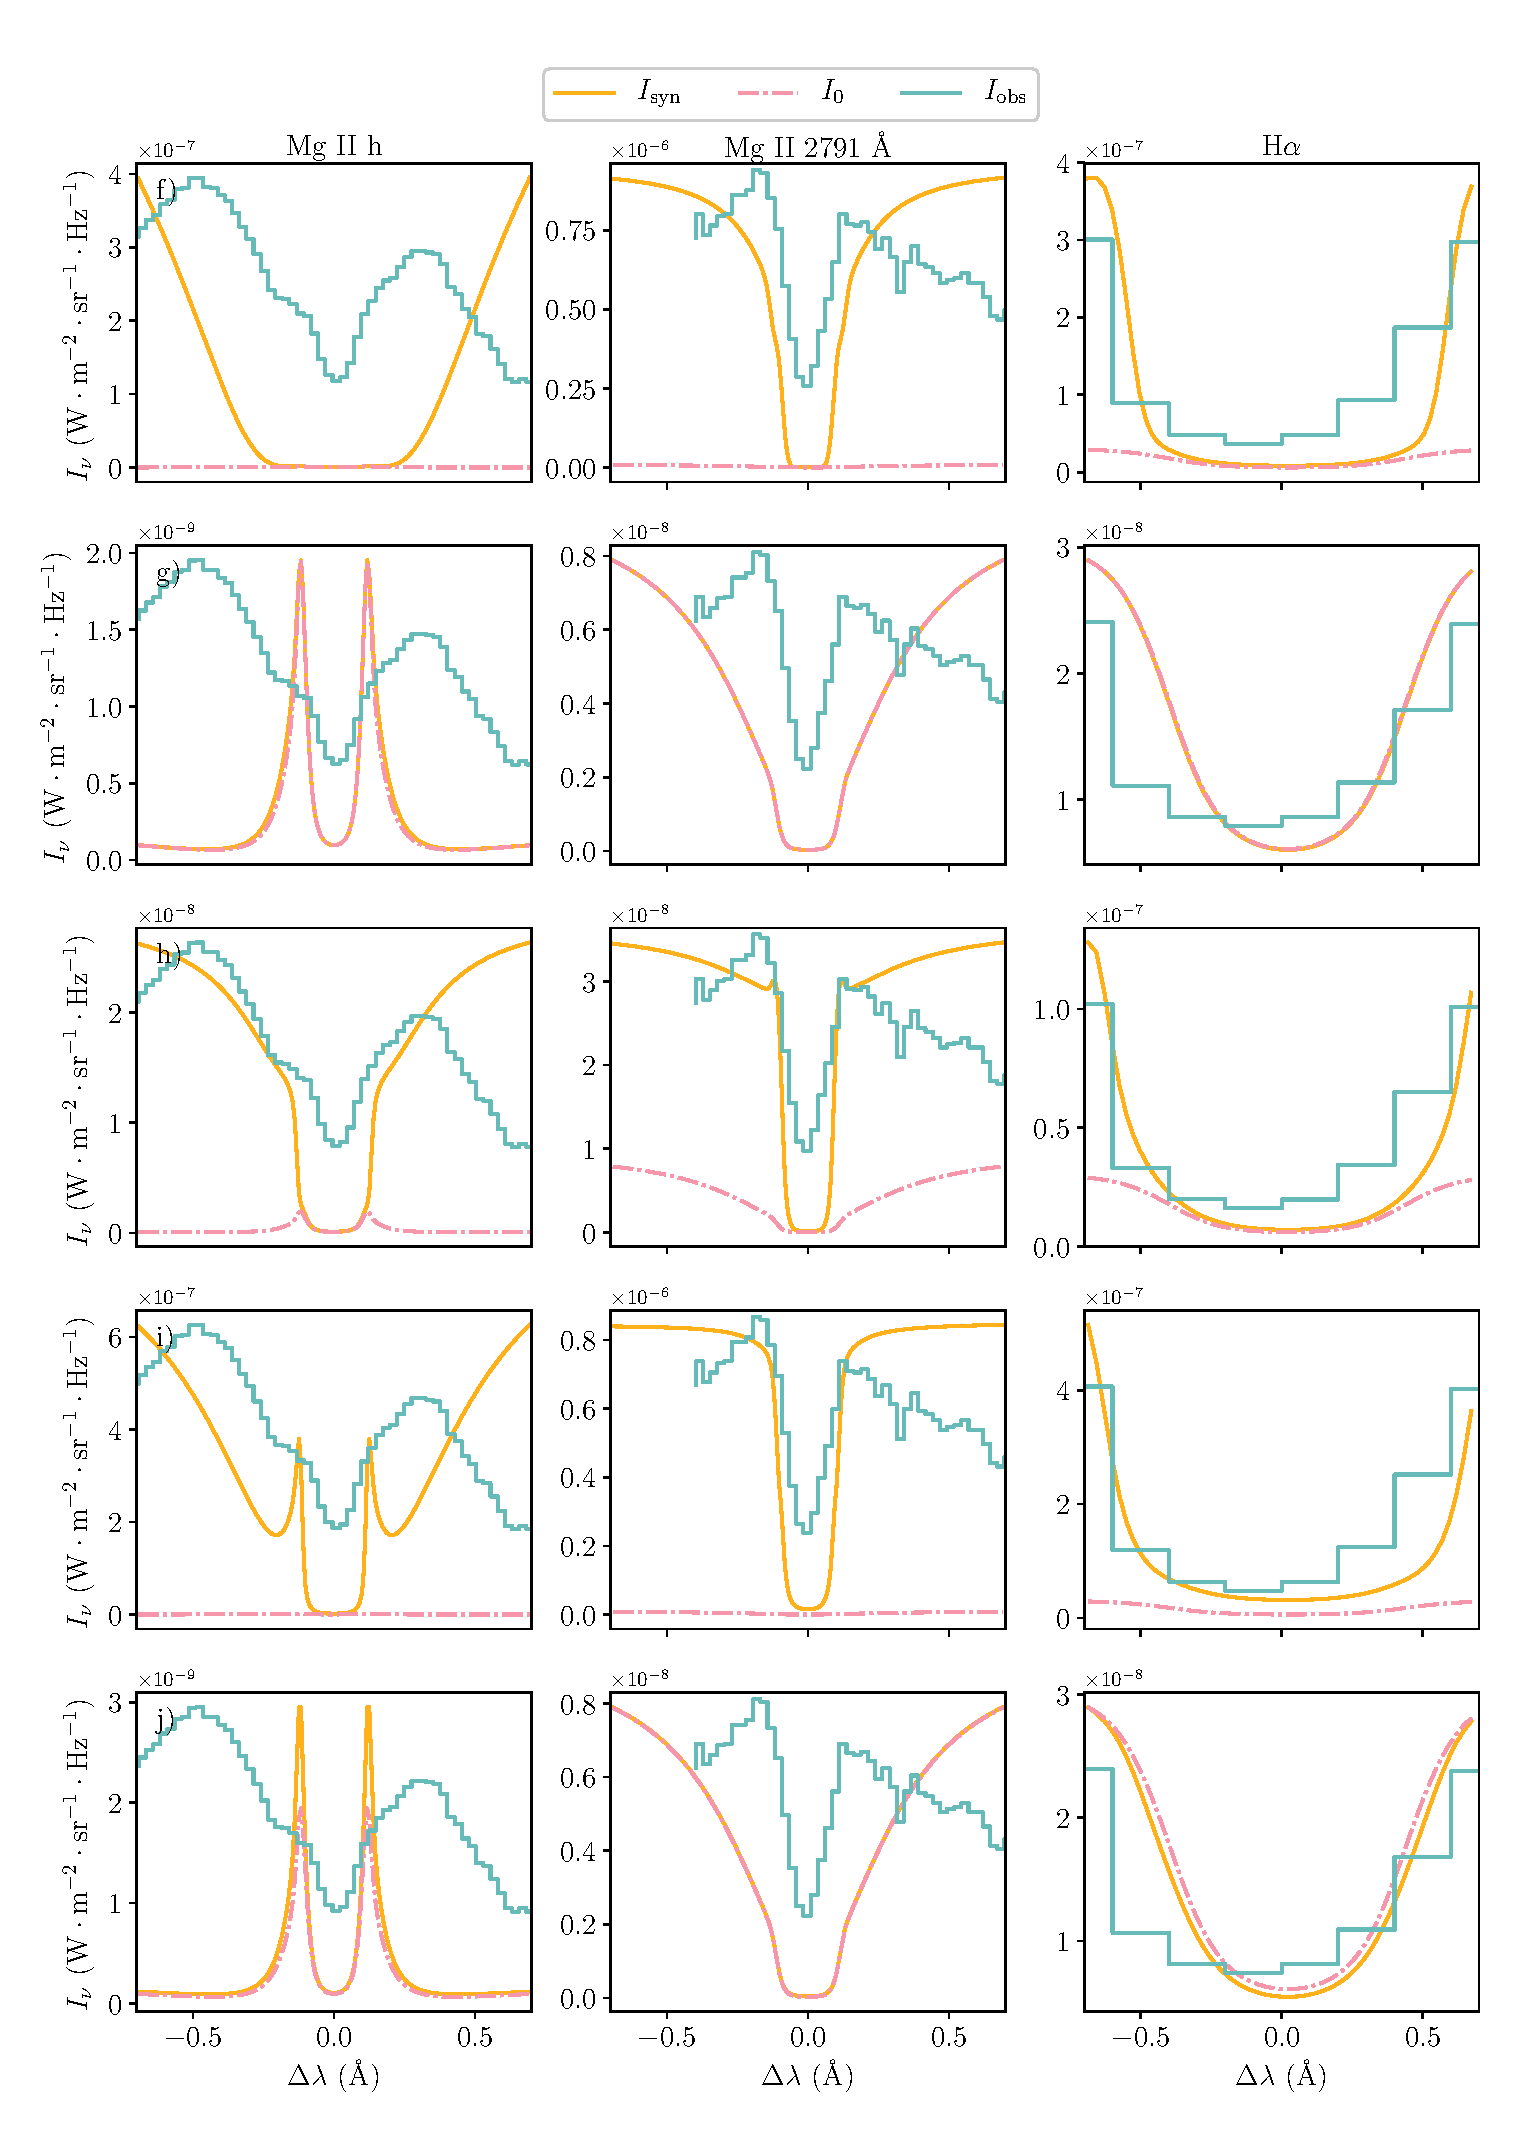
\includegraphics[width=\textwidth]{figs/UVB_spec_2}
	\caption{RH代码模拟得到的低层大气加热后的Mg \textsc{ii} h,2791 \mbox{\AA}及H$\alpha$线的谱线轮廓与IRIS卫星等观测的对比图(其二)。粉色点划线轮廓代表了初始谱线轮廓;黄色实线代表调整后计算得到的谱线轮廓。蓝色阶梯线代表实际观测的紫外爆发(Mg \textsc{ii})和Ellerman炸弹(H$\alpha$)的谱线轮廓。}
	\label{fig:5.3}
\end{figure}

\begin{figure}
	\centering
	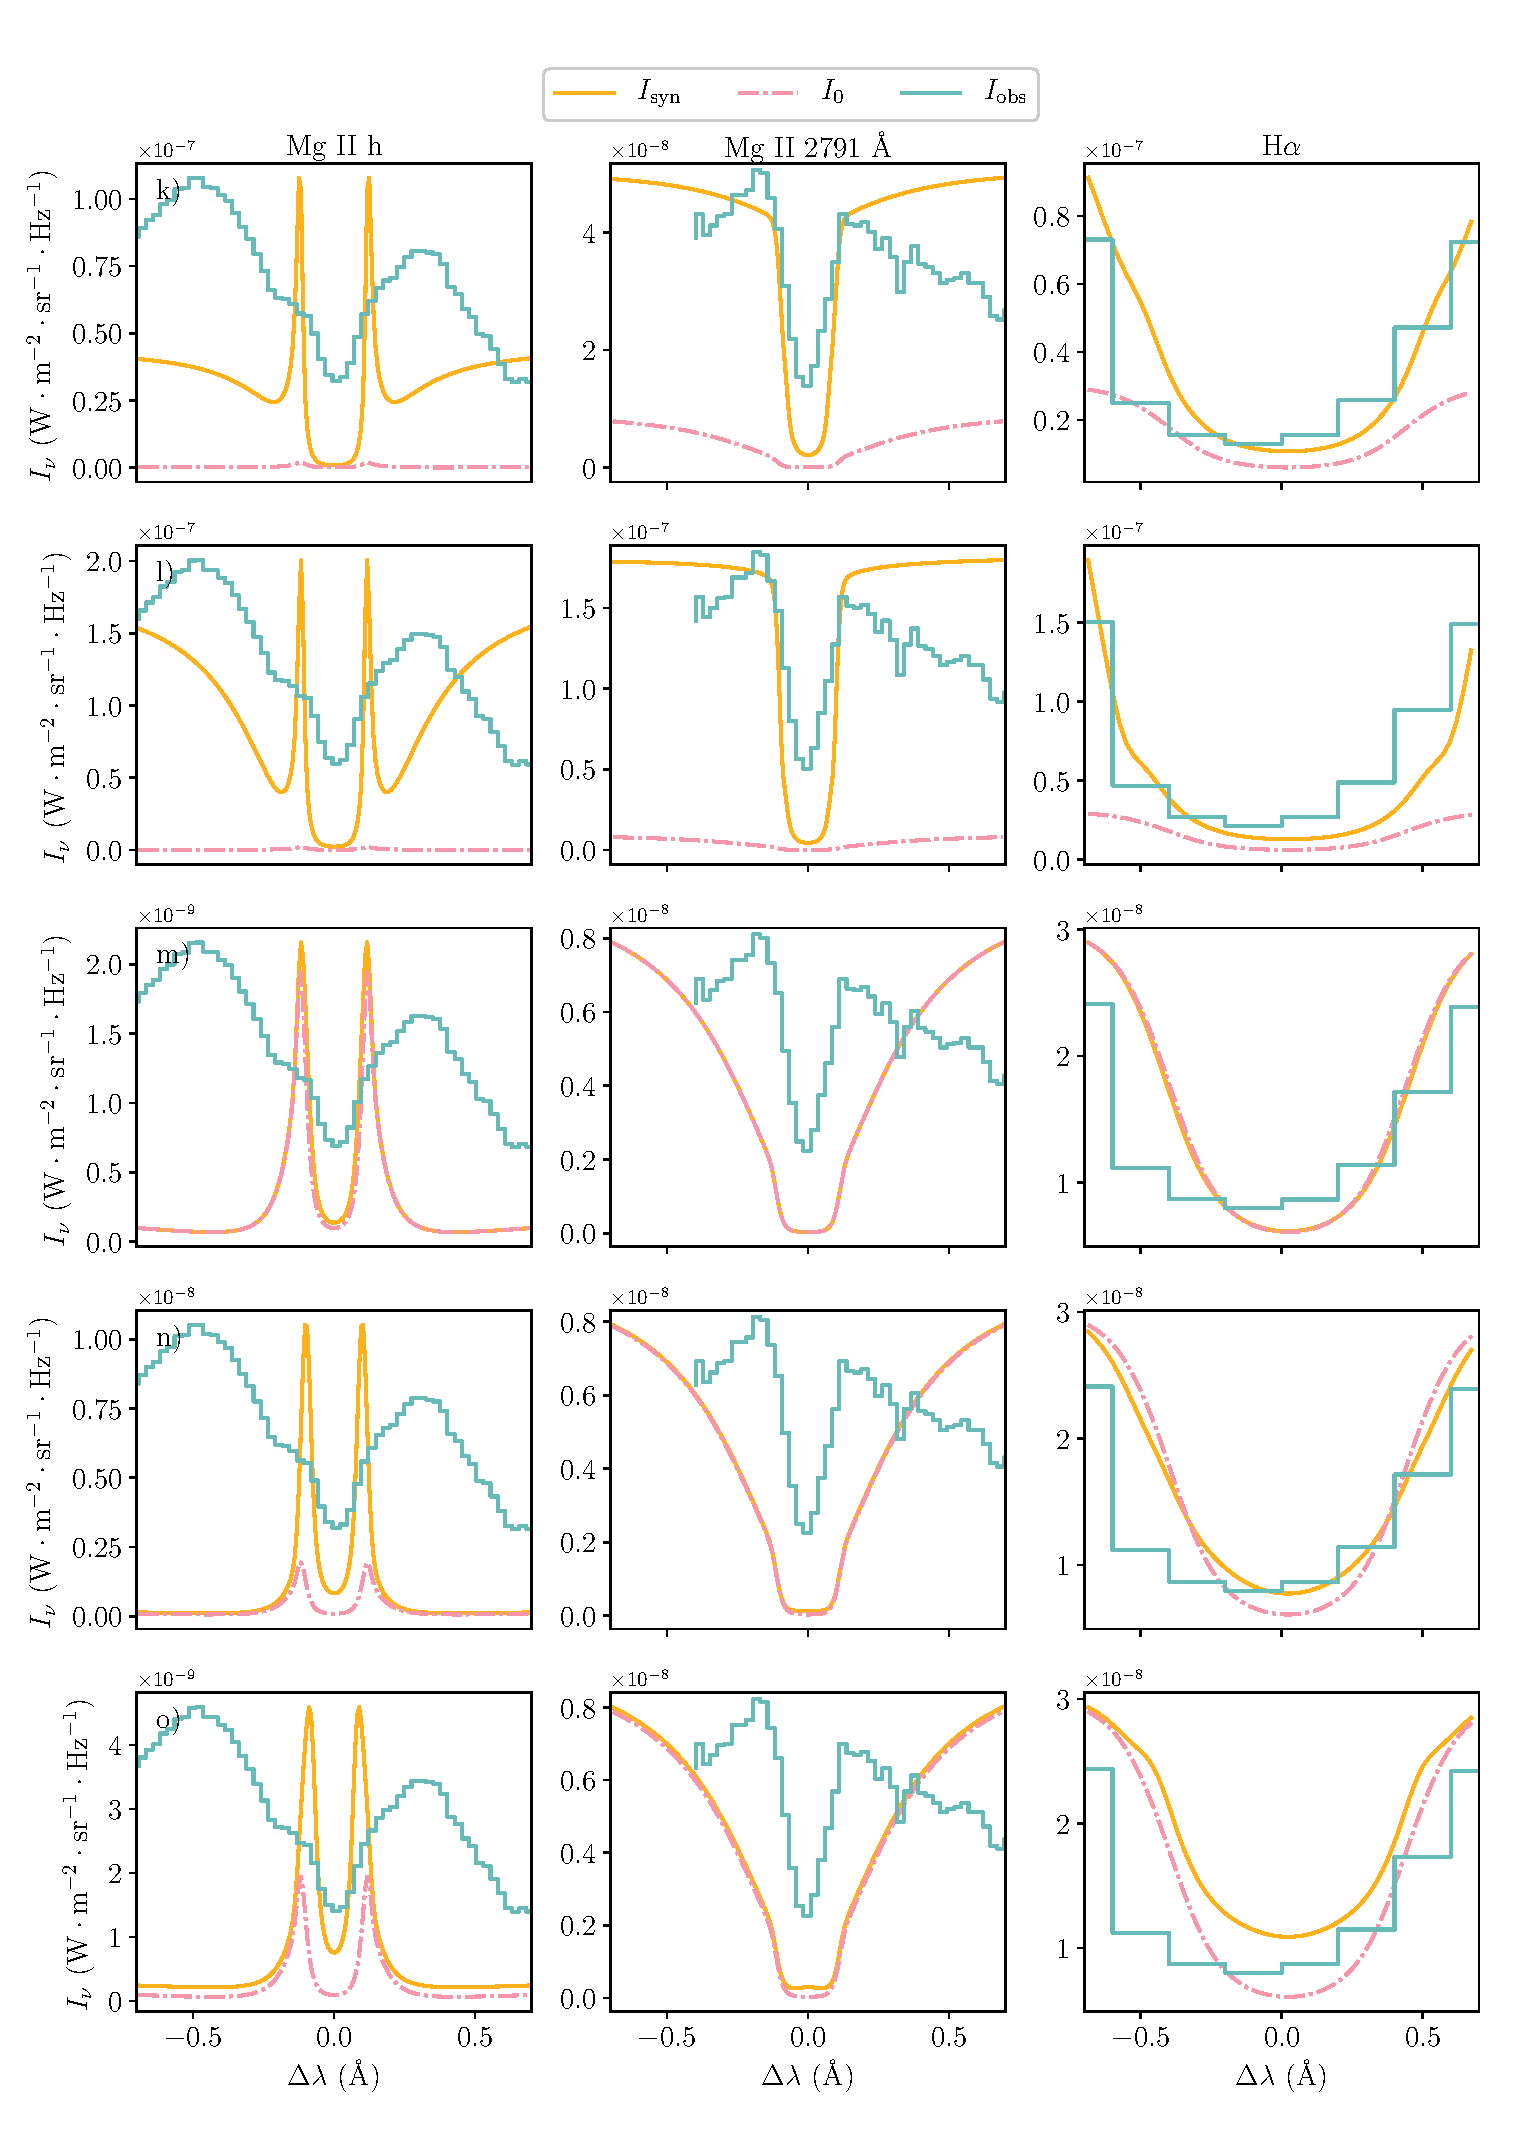
\includegraphics[width=\textwidth]{figs/UVB_spec_3}
	\caption{RH代码模拟得到的低层大气加热后的Mg \textsc{ii} h,2791 \mbox{\AA}及H$\alpha$线的谱线轮廓与IRIS卫星等观测的对比图(其三)。粉色点划线轮廓代表了初始谱线轮廓;黄色实线代表调整后计算得到的谱线轮廓。蓝色阶梯线代表实际观测的紫外爆发(Mg \textsc{ii})和Ellerman炸弹(H$\alpha$)的谱线轮廓。}
	\label{fig:5.4}
\end{figure}
% vim:ts=4:sw=4
	% 结论。
	% Copyright (c) 2014,2016 Casper Ti. Vector
% Public domain.

\chapter{结论}\label{chap:con}
本文通过一维辐射流体力学代码RADYN和一维辐射转移代码RH进行了一系列太阳和M矮星上爆发活动的模拟,包含由观测数值驱动的太阳上的X级耀斑的5F11非热电子加热模拟,对M矮星上发生的白光耀斑的不同非热电子束加热的参数研究,以及对太阳上的低高度和小尺度的爆发活动的半经验的模拟。尽管有些模拟过程非常的简单粗暴和直接,但是我们仍然从这些数值模拟当中发现了一些有趣的结论:
\begin{enumerate}
	\item 我们在RH代码中引入了新的Stark致宽计算方法,并发现对于Mg \textsc{ii}谱线仍需要在Stark宽度上乘上一个30倍的因子才能较好的再现Mg \textsc{ii} h,k和三重线在耀斑带上远线翼出现剧烈辐射增强的谱线轮廓。对于C \textsc{ii}远线翼的辐射,我们同样可以通过人为增大其Stark致宽效应来在远线翼上产生和观测拟合较好的谱线轮廓。这些因子可能来源于非热电子对Stark致宽的贡献和对大气电子密度的错误计算等原因。
	\item 我们首次在自洽的大气中计算得到了单发射峰的非线心反转的Mg \textsc{ii} h和k线,它们的线心形成于高度压缩的过渡区下电子密度约为$8\times 10^{14}\ \mathrm{cm^{-3}}$的区域内。如此高的电子密度保证了线心形成范围内的近似局部热动平衡,使谱线不再出现线心反转的轮廓。
	\item 我们发现Mg \textsc{ii}三重线的形成高度在模拟耀斑衰减相时线心形成高度和Mg \textsc{ii} h和k线非常相近,因此它们在耀斑过程中可能不再是低色球加热的良好定量诊断。
	\item 我们的5F11模拟能够较好地再现Mg \textsc{ii} h和k线在耀斑观测中的演变过程,从出现蓝翼增强到产生较大红移再到红移减小出现非线心反转谱线的过程。这个蓝翼增强来自于上流较冷($\sim 4\times10^4$ K)物质造成的蓝翼不透明度增强,支持了\textcites{Tei2018}观测到类似Mg \textsc{ii} h和k线的蓝翼增强的解释。
	\item 我们的模拟不能同时再现其他色球谱线如C \textsc{ii}和Si \textsc{iv}同时的演化过程,主要的问题可能来自于RADYN本身对冷却过程的处理不够完善以及我们没有在RH中使用同时包含Si \textsc{i}-\textsc{v}能级的Si原子模型。
	\item 在人工添加一个z方向的磁场后,我们利用RH模拟了He \textsc{iv} 10830 \mbox{\AA}谱线的Stokes参数在5F11模型中的演化过程。作为形成在高色球的谱线,He \textsc{i} 10830同样出现了较大红移的谱线轮廓。其Stokes参数$V/I$相比C级耀斑观测值稍大。
	\item 我们对不同非热电子束加热的M矮星耀斑模拟中的Mg \textsc{ii}谱线轮廓与形成高度进行了较为完备的分析。我们发现能够再现白光连续谱观测的非热电子束参数1F13$E_c85$加热的模拟大气并不能较好地再现Mg \textsc{ii}谱线轮廓。反而是另外两个1F11$E_c85$和1F13$E_c350$分别产生了类似于\textcites{Hawley2007}中观测到的蓝翼增强和红翼增强的谱线。
	\item 我们发现在M矮星中Mg \textsc{ii}三重线的线心形成高度在宁静大气中就已经和Mg \textsc{ii} h和k线接近,但是Mg \textsc{ii}三重线的线翼形成在更深的位置,它们的线翼辐射都对高截止能量$E_c$的电子束加热非常敏感。
	\item 我们利用手动在VALC大气中插入局部温度上升研究了不同高度不同程度加热对Mg \textsc{ii}和H$\alpha$谱线的影响。我们发现Ellerman炸弹光谱中出现的Mg \textsc{ii}线线翼增强可能需要在0.25-1.0 Mm的范围内有局部温度升高至接近$10^4$ K。
	\item 我们在低高度小尺度加热的模拟中发现了与\textcites{Hong2017b}类似存在低层大气温度升高时H$\alpha$谱线线心线翼强度减弱的情况。
\end{enumerate}


% vim:ts=4:sw=4


	% 正文中的附录部分。
	\appendix
	% 排版参考文献列表。bibintoc 选项使“参考文献”出现在目录中;
	% 如果同时要使参考文献列表参与章节编号,可将“bibintoc”改为“bibnumbered”。
	\printbibliography[heading = bibintoc]
	% 各附录。
	% Copyright (c) 2014,2016 Casper Ti. Vector
% Public domain.

\chapter{对RH代码的修改与讨论}
\section{对RH代码的修改}
在附录的这一章节,我将简单介绍我对RH代码的一些修改。相关修改的方法和文件已经上传到GitHub上,有需要的读者可以从下面的链接访问这些内容。
\subsection{嵌入STARK-B数据库结果}
对于Stark致宽的修改全部集中在RH主文件夹的\texttt{broad.c},具体其实非常傻瓜就是找到你要修改的能级,然后把它的Stark致宽计算公式修改成你想要的。这里提供了我修改了Mg \textsc{ii} h,k还有三重线Stark致宽的\texttt{broad.c}文件:

\url{https://github.com/nightmarein13/RH-SB}
\subsection{提供辐射流量输出}
RH1D代码中原本是存在辐射流量输出的(或者说一开始就设计成先求解辐射流量,如果有需求再去求解辐射强度),但是RH1.5D不知道为什么莫名其妙把它给删了,可能是Tiago觉得算太阳没必要看辐射流量?但是对于恒星耀斑的计算辐射流量还是相当重要的,因此需要花一些功夫把它加回来。具体的流程写在这个里面了:

\url{https://github.com/nightmarein13/my_toys/blob/master/add_flux.md}

修改后会在输出的HDF5文件中多生成一个名为\texttt{flux}的\texttt{dataset}。如果你使用Tiago提供的\texttt{helita}库中的\texttt{rh15d.Rh15dout()}类来读取输出,那么会自动在\texttt{ray}下生成一个名为\texttt{flux}的\texttt{xarray.DataArray}。
\subsection{用于修改大气的可视化Ipython Notebook}\label{sec:a.1.3}
大致是长图~\ref{fig:a.1.2}这个样子的,可以对温度、电子密度、一维速度和微湍动速度做一个简单(简陋)的调节。代码内容大量参考\texttt{helita}库中的\texttt{rh15d\_vis.InputAtmosphere()}类。下载地址:

\url{https://github.com/nightmarein13/my_toys/blob/master/rh15d_edit_atmos.py}

\begin{figure}
	\centering
	\includegraphics[width=\textwidth]{figs/naive}
	\caption{简陋的不能再简陋的可视化调节程序。。原谅我warning太多}
	\label{fig:a.1.2}
\end{figure}

\section{RH对Mg \textsc{ii}的Stark致宽的处理究竟有哪些问题?}\label{sec:a.2}
你要是问我到底该怎么算Stark致宽最好,那肯定从量子力学出发最好,但是毕竟像我这种不自量力的人是不会从微扰论出发算那么多矩阵元来求整个致宽问题的。因此我觉得有一些经典近似其实是很正常的。那么RH所做的经典碰撞近似究竟出了哪些问题呢?

根据\textcites{Mihalas2014}经典碰撞必须要满足三个条件才可能成立:

\textbf{碰撞持续时间和碰撞间隔的比较}

首先我们得定义一下碰撞持续时间,是碰撞过程中的总相移$\eta(\rho)$除以碰撞中最近时刻的频率移动,即\parencites{Mihalas2014}:
\begin{equation}
	\tau_{s}=\frac{\eta\left(\rho_{0}\right)}{\Delta \omega\left(\rho_{0}\right)}=\frac{\pi}{2} \cdot \frac{\rho_{0}}{v_{r e l}}
\end{equation}
其中等效瞄准距离$\rho_{0}=\left(\pi C_{4} / 2 v_{r e l}\right)^{1 / 3}$。

在碰撞近似之中,我们每次只考虑一个碰撞粒子对辐射粒子的作用,因此你的碰撞持续时间应该远小于碰撞间隔,即$\tau_s \ll \tau $。简单的来说就是你的等效瞄准距离$\rho_0$要比平均每个辐射粒子之间的间距$r_0$要小很多。对于Mg \textsc{ii}线心形成高度来说,$n_e \sim 10^{14}\ \mathrm{cm^{-3}}$,因此平均距离$r_0 \sim 10^{-5}\ \mathrm{cm}$。当我们取$T\sim 2\times 10^4$ K时,$\rho\sim 10^{-7}\ \mathrm{cm^{-3}}$。可见这条还是满足的,不然的话在经典框架内就只能去用统计理论算Holtzmark分布了。

\textbf{碰撞过程中的辐射}

碰撞近似忽略了碰撞过程中粒子发出的辐射,而这些辐射由于是在能级被扰动的情况下发出的,因此更有可能在线翼上,因此在远线翼上用碰撞近似本来就是不太好的,应该使用统计理论。一个典型的计算两个理论使用范围的分界频率是\parencites{Mihalas2014}:
\begin{equation}
	\Delta \omega_{c}=\frac{v_{r e l}^{4 / 3}}{(\pi / 2)^{4} C_{4}^{1 / 3}}
\end{equation}
对于电子产生的Stark致宽来说$\Delta \omega_{c}$远大于整个谱线轮廓,而对于离子来说如过取$C_4 \sim 10^{-14}-10^{-16}\ \mathrm{cm^4\cdot s^{-1}}$,$\Delta \omega_{c}\sim 0.5 -2.0$ \mbox{\AA}。因此其实Mg \textsc{ii}受离子的Stark致宽应该用统计理论来算,不过鉴于它相对于电子其实贡献并不多,可以暂时忽略。

\textbf{绝热近似}

由于碰撞理论是个纯经典的理论,我们希望整个碰撞持续时间所对应的频率$\omega_s = 1/\tau_s$要远远小于量子跃迁的频率,即\parencites{Mihalas2014}:
\begin{equation}
	\Delta \omega_{s} \ll \frac{E_{j}-E_{i}}{\hbar}
\end{equation}
对于Mg \textsc{ii}由自由电子引起的Stark效应,$\omega_s\sim 10^{15}\ \mathrm{rad\cdot s^{-1}}$。而Mg \textsc{ii} h和k线跃迁频率$\omega_{ij}\sim 6.7\times 10^{15}\ \mathrm{rad\cdot s^{-1}}$。两者在同一个量级上,所以我们认为绝热近似这个条件在此时是不满足的,还是需要引入STARK-B中考虑了部分量子力学效应的半经典理论来计算。



% vim:ts=4:sw=4

	% Copyright (c) 2014,2016 Casper Ti. Vector
% Public domain.

\chapter{本科期间的主要工作和成果}
\noindent
\textbf{本研基金}

国家创新训练项目\ 指导老师:田晖研究员

\noindent
\textbf{发表论文}

Yingjie Zhu, Adam F. Kowalski, Hui Tian, Han Uitenbroek et al. \emph{"Modeling Mg II h, k and Triplet Lines at Solar Flare Ribbons"}, accepted by \emph{ApJ}, 2019

\noindent
\textbf{会议海报}

第四届中国华人空间天气大会(The $4^{\mathrm{th}}$ International Space Weather Conference, 2017, Beijing, China): \emph{"An S-shape flare ribbon observed with NVST and SDO/AIA"} 

第二届中欧太阳物理会议($2^{\mathrm{nd}}$ China-Europe Solar Physics Meeting, 2019, Hvar, Croatia): Outstanding Student Poster Award \emph{"Modeling Mg II h, k and Triplet Lines at Solar Flare Ribbons"} 

\noindent
\textbf{会议口头报告}

2017年中国地球物理年会(The 2017 Annual Meeting of Chinese Geoscience Union, 2017, Beijing, China): \emph{"An S-shape flare ribbon observed with NVST and SDO/AIA"} 

国际空间科学研究院-北京国际小组讨论会:利用耀斑带光谱观测诊断太阳耀斑的加热机制(ISSI/ISSI-BJ International Team Workshop: Diagnosing heating mechanism in solar flares through spectroscopic observations of flare ribbons, 2018, Beijing, China): \emph{"Modeling Mg II h, k and Triplet Lines at Solar Flare Ribbons"} 
% vim:ts=4:sw=4

	% 以下为正文之后的部分,默认不进行章节编号。
	\backmatter
	% 致谢。
	% Copyright (c) 2014,2016 Casper Ti. Vector
% Public domain.

\chapter{致谢}
我首先要感谢我的本科生科研导师田晖研究员在太阳物理研究领域提供的指导和帮助,同时提供了我与其他研究人员交流讨论学习的机会。特别是在IRIS卫星数据处理,谱线在不同情况下的形态特征等技能知识方面的指导。

本论文的部分工作是作者在2018年7-8月间于美国科罗拉多大学博尔德分校(\textit{University of Colorado Boulder})的国家太阳天文台(\textit{National Solar Observatory})访问交流时完成的。我非常感谢美国科罗拉多大学博尔德分校和国家太阳天文台的助理教授Adam. F. Kowalski与美国国家太阳天文台的天文学家Han Uitenbroek博士对我在辐射流体力学模拟,RADYN,RH代码使用等一系列问题上的帮助。我也要感谢北京大学本科生科研项目中的国家创新训练项目为我提供的资助。

作者还要感谢挪威奥斯陆大学(\textit{University of Oslo})的Mats Carlsson教授与作者在RADYN模拟及谱线致宽上的讨论,中科院紫金山天文台李瑛研究员和南京大学天文与空间科学学院洪杰博士对作者在辐射流体力学模拟方面的帮助以及美国NASA Goddard航天中心的Graham Kerr博士与作者在Si \textsc{iv}谱线模拟方面建设性的讨论。作者还要感谢ISSI/ISSI-BJ国际小组讨论会的全体参会人员,包括NASA Goddard航天中心Joel C. Allred博士,瑞士西北应用科学大学(\textit{University of Applied Sciences and Arts Northwestern Switzerland})的Lucia Kleint博士,捷克科学院(\textit{The Czech Academy of Sciences})的Petr Heinzel博士和日本京都大学(\textit{Kyoto University})的Akiko Tei博士等。

同时我要感谢北京大学科维理天文与天体物理研究所的Gregory J. Herczeg教授对我在恒星结构与演化知识学习的帮助和北京大学天文系的刘富坤教授开设的《理论天体物理》课程对我在辐射转移相关知识学习的帮助。

此外,我感谢田晖教授研究组中的Tanmoy Samanta,宋永亮,陈亚杰,张婧雯,谭光钰,朱瑞学长学姐,陈雨豪同学,高宇航学弟对我在本科生科研以及毕业论文中的帮助,特别是陈亚杰学长提供了紫外爆发和Ellerman炸弹的一系列光谱数据。我还要感谢我的室友赵辰兴宇,李京寰,刘立超,以及北京大学地球与空间科学学院2015级本科4班全体同学对我学习和生活上的帮助。

特别地,我还要感谢杨子浩同学在这两年本科生科研过程中给予我的帮助、支持、鼓励和启迪。他踏实认真严谨好学勤奋的研究态度一直是我学习的榜样。同时非常感谢他通读了我的论文,在文字修改上提出了很多重要的意见。

我感谢Github上的开发者Casper Ti. Vector(\href{mailto:CasperVector@gmail.com}{CasperVector@gmail.com})提供的\LaTeX 模板pkuthss对我论文排版提供的帮助。

最后我要感谢我的家人,尤其是我的母亲和奶奶对我的关心信任帮助对我一直以来恶劣性格和抑郁情绪的无限包容。没有她们我可能活不到今天。

%我还要在这里特地感谢我的女朋友王怡媛这一年多来在我情绪低落和陷入困境时给我的支持,帮助我一直走到现在。
% vim:ts=4:sw=4

	% 原创性声明和使用授权说明。
	% Copyright (c) 2008-2009 solvethis
% Copyright (c) 2010-2017 Casper Ti. Vector
% All rights reserved.
%
% Redistribution and use in source and binary forms, with or without
% modification, are permitted provided that the following conditions are
% met:
%
% * Redistributions of source code must retain the above copyright notice,
%   this list of conditions and the following disclaimer.
% * Redistributions in binary form must reproduce the above copyright
%   notice, this list of conditions and the following disclaimer in the
%   documentation and/or other materials provided with the distribution.
% * Neither the name of Peking University nor the names of its contributors
%   may be used to endorse or promote products derived from this software
%   without specific prior written permission.
%
% THIS SOFTWARE IS PROVIDED BY THE COPYRIGHT HOLDERS AND CONTRIBUTORS "AS
% IS" AND ANY EXPRESS OR IMPLIED WARRANTIES, INCLUDING, BUT NOT LIMITED TO,
% THE IMPLIED WARRANTIES OF MERCHANTABILITY AND FITNESS FOR A PARTICULAR
% PURPOSE ARE DISCLAIMED. IN NO EVENT SHALL THE COPYRIGHT HOLDER OR
% CONTRIBUTORS BE LIABLE FOR ANY DIRECT, INDIRECT, INCIDENTAL, SPECIAL,
% EXEMPLARY, OR CONSEQUENTIAL DAMAGES (INCLUDING, BUT NOT LIMITED TO,
% PROCUREMENT OF SUBSTITUTE GOODS OR SERVICES; LOSS OF USE, DATA, OR
% PROFITS; OR BUSINESS INTERRUPTION) HOWEVER CAUSED AND ON ANY THEORY OF
% LIABILITY, WHETHER IN CONTRACT, STRICT LIABILITY, OR TORT (INCLUDING
% NEGLIGENCE OR OTHERWISE) ARISING IN ANY WAY OUT OF THE USE OF THIS
% SOFTWARE, EVEN IF ADVISED OF THE POSSIBILITY OF SUCH DAMAGE.

{
	\ctexset{section = {
		format+ = {\centering}, beforeskip = {40bp}, afterskip = {15bp}
	}}

	% 学校书面要求本页面不要页码,但在给出的 Word 模版中又有页码且编入了目录。
	% 此处以 Word 模版为实际标准进行设定。
	\specialchap{北京大学学位论文原创性声明和使用授权说明}
	\mbox{}\vspace*{-3em}
	\section*{原创性声明}

	本人郑重声明:
	所呈交的学位论文,是本人在导师的指导下,独立进行研究工作所取得的成果。
	除文中已经注明引用的内容外,
	本论文不含任何其他个人或集体已经发表或撰写过的作品或成果。
	对本文的研究做出重要贡献的个人和集体,均已在文中以明确方式标明。
	本声明的法律结果由本人承担。
	\vskip 1em
	\rightline{%
		论文作者签名:\hspace{5em}%
		日期:2019年6月10日%
	}

	\section*{%
		学位论文使用授权说明\\[-0.33em]
		\textmd{\zihao{5}(必须装订在提交学校图书馆的印刷本)}%
	}

	本人完全了解北京大学关于收集、保存、使用学位论文的规定,即:
	\begin{itemize}
		\item 按照学校要求提交学位论文的印刷本和电子版本;
		\item 学校有权保存学位论文的印刷本和电子版,
			并提供目录检索与阅览服务,在校园网上提供服务;
		\item 学校可以采用影印、缩印、数字化或其它复制手段保存论文;
		\item 因某种特殊原因需要延迟发布学位论文电子版,
			授权学校在 $\Box$\nobreakspace{}一年 /
			$\Box$\nobreakspace{}两年 /
			$\Box$\nobreakspace{}三年以后在校园网上全文发布。
	\end{itemize}
	\centerline{(保密论文在解密后遵守此规定)}
	\vskip 1em
	\rightline{%
		论文作者签名:\hspace{5em}导师签名:\hspace{5em}%
		日期:2019年6月10日%
	}

	% 若需排版二维码,请将二维码图片重命名为“barcode”,
	% 转为合适的图片格式,并放在当前目录下,然后去掉下面 2 行的注释。
	%\vfill\noindent
	%\includegraphics[height = 5em]{barcode}
}

% vim:ts=4:sw=4

\end{document}

% vim:ts=4:sw=4
